%%%%%%%%%%%%%%%%%%%%%%%%%%%%%%%%%%%%%%%%%
% Masters/Doctoral Thesis 
% LaTeX Template
% Version 2.5 (27/8/17)
%
% This template was downloaded from:
% http://www.LaTeXTemplates.com
%
% Version 2.x major modifications by:
% Vel (vel@latextemplates.com)
%
% This template is based on a template by:
% Steve Gunn (http://users.ecs.soton.ac.uk/srg/softwaretools/document/templates/)
% Sunil Patel (http://www.sunilpatel.co.uk/thesis-template/)
%
% Template license:
% CC BY-NC-SA 3.0 (http://creativecommons.org/licenses/by-nc-sa/3.0/)
%
%%%%%%%%%%%%%%%%%%%%%%%%%%%%%%%%%%%%%%%%%

%----------------------------------------------------------------------------------------
%	PACKAGES AND OTHER DOCUMENT CONFIGURATIONS
%----------------------------------------------------------------------------------------

\documentclass[
11pt, % The default document font size, options: 10pt, 11pt, 12pt
%oneside, % Two side (alternating margins) for binding by default, uncomment to switch to one side
english, % ngerman for German
singlespacing, % Single line spacing, alternatives: onehalfspacing or doublespacing
%draft, % Uncomment to enable draft mode (no pictures, no links, overfull hboxes indicated)
%nolistspacing, % If the document is onehalfspacing or doublespacing, uncomment this to set spacing in lists to single
%liststotoc, % Uncomment to add the list of figures/tables/etc to the table of contents
%toctotoc, % Uncomment to add the main table of contents to the table of contents
%parskip, % Uncomment to add space between paragraphs
%nohyperref, % Uncomment to not load the hyperref package
headsepline, % Uncomment to get a line under the header
%chapterinoneline, % Uncomment to place the chapter title next to the number on one line
%consistentlayout, % Uncomment to change the layout of the declaration, abstract and acknowledgements pages to match the default layout
]{MastersDoctoralThesis} % The class file specifying the document structure

\usepackage[utf8]{inputenc} % Required for inputting international characters
\usepackage[T1]{fontenc} % Output font encoding for international characters

\usepackage{mathpazo} % Use the Palatino font by default

\usepackage[backend=bibtex,style=numeric,natbib=true]{biblatex} % Use the bibtex backend with the authoryear citation style (which resembles APA)


\addbibresource{Bib/example.bib} % The filename of the bibliography

\usepackage[autostyle=true]{csquotes} % Required to generate language-dependent quotes in the bibliography
\usepackage{verbatim}
\usepackage{xspace}
\usepackage{placeins}
\usepackage{subfig}
\usepackage{parskip}
% custom-commands.tex
\newcommand{\tty}{$t\bar{t}\gamma$ }
\newcommand{\ttbar}{$t\bar{t}$ }
\newcommand{\photon}{$\gamma$ }
\newcommand{\cme}{$\sqrt{s} = 13 \mathrm{TeV}$ }


\usepackage{Others/atlasmisc}
\usepackage{Others/atlasunit}


%----------------------------------------------------------------------------------------
%	MARGIN SETTINGS
%----------------------------------------------------------------------------------------

\geometry{
	paper=a4paper, % Change to letterpaper for US letter
	inner=2.5cm, % Inner margin
	outer=3.8cm, % Outer margin
	bindingoffset=.5cm, % Binding offset
	top=1.5cm, % Top margin
	bottom=1.5cm, % Bottom margin
	%showframe, % Uncomment to show how the type block is set on the page
}

%----------------------------------------------------------------------------------------
%	THESIS INFORMATION
%----------------------------------------------------------------------------------------

\thesistitle{Measurement of differential cross-sections of \tty process with ATLAS detector} % Your thesis title, this is used in the title and abstract, print it elsewhere with \ttitle
\supervisor{PD. Dr. Carmen \textsc{Diez Pardos}} % Your supervisor's name, this is used in the title page, print it elsewhere with \supname
\examiner{} % Your examiner's name, this is not currently used anywhere in the template, print it elsewhere with \examname
\degree{Doctor of Philosophy} % Your degree name, this is used in the title page and abstract, print it elsewhere with \degreename
\author{Buddhadeb \textsc{Mondal}} % Your name, this is used in the title page and abstract, print it elsewhere with \authorname
\addresses{} % Your address, this is not currently used anywhere in the template, print it elsewhere with \addressname

\subject{physical Sciences} % Your subject area, this is not currently used anywhere in the template, print it elsewhere with \subjectname
\keywords{} % Keywords for your thesis, this is not currently used anywhere in the template, print it elsewhere with \keywordnames
\university{\href{http://www.uni-siegen.de}{Universität Siegen}} % Your university's name and URL, this is used in the title page and abstract, print it elsewhere with \univname
\department{\href{http://hep.physik.uni-siegen.de}{Center for Particle Physics}} % Your department's name and URL, this is used in the title page and abstract, print it elsewhere with \deptname
\group{\href{http://researchgroup.university.com}{Research Group Name}} % Your research group's name and URL, this is used in the title page, print it elsewhere with \groupname
\faculty{\href{http://faculty.university.com}{Faculty IV}} % Your faculty's name and URL, this is used in the title page and abstract, print it elsewhere with \facname

\AtBeginDocument{
\hypersetup{pdftitle=\ttitle} % Set the PDF's title to your title
\hypersetup{pdfauthor=\authorname} % Set the PDF's author to your name
\hypersetup{pdfkeywords=\keywordnames} % Set the PDF's keywords to your keywords
}

\usepackage{amsmath}
\usepackage{hyperref}
\usepackage{cleveref}
\Crefname{section}{Section}{Sections}
\Crefname{figure}{Figure}{Figures}
\Crefname{table}{Table}{Tables}
\Crefname{equation}{Equation}{Equations}
\hfuzz=5.002pt 


\begin{document}

\frontmatter % Use roman page numbering style (i, ii, iii, iv...) for the pre-content pages

\pagestyle{plain} % Default to the plain heading style until the thesis style is called for the body content

%----------------------------------------------------------------------------------------
%	TITLE PAGE
%----------------------------------------------------------------------------------------

\begin{titlepage}
\begin{center}

\vspace*{.06\textheight}
{\scshape\LARGE \univname\par}\vspace{1.5cm} % University name
\textsc{\Large Doctoral Thesis}\\[0.5cm] % Thesis type

\HRule \\[0.4cm] % Horizontal line
{\huge \bfseries \ttitle\par}\vspace{0.4cm} % Thesis title
\HRule \\[1.5cm] % Horizontal line
 
\begin{minipage}[t]{0.4\textwidth}
\begin{flushleft} \large
\emph{Author:}\\
\href{}{\authorname} % Author name - remove the \href bracket to remove the link
\end{flushleft}
\end{minipage}
\begin{minipage}[t]{0.4\textwidth}
\begin{flushright} \large
\emph{Supervisor:} \\
\href{}{\supname} % Supervisor name - remove the \href bracket to remove the link  
\end{flushright}
\end{minipage}\\[3cm]
 
\vfill

\large \textit{A thesis submitted in fulfillment of the requirements\\ for the degree of \degreename}\\[0.3cm] % University requirement text
\textit{in the}\\[0.4cm]
\groupname\\\deptname\\[2cm] % Research group name and department name
 
\vfill

{\large \today}\\[4cm] % Date
%\includegraphics{Logo} % University/department logo - uncomment to place it
 
\vfill
\end{center}
\end{titlepage}

%----------------------------------------------------------------------------------------
%	DECLARATION PAGE
%----------------------------------------------------------------------------------------

\begin{declaration}
\addchaptertocentry{\authorshipname} % Add the declaration to the table of contents
\noindent I, \authorname, declare that this thesis titled, \enquote{\ttitle} and the work presented in it are my own. I confirm that:

\begin{itemize} 
\item This work was done wholly or mainly while in candidature for a research degree at this University.
\item Where any part of this thesis has previously been submitted for a degree or any other qualification at this University or any other institution, this has been clearly stated.
\item Where I have consulted the published work of others, this is always clearly attributed.
\item Where I have quoted from the work of others, the source is always given. With the exception of such quotations, this thesis is entirely my own work.
\item I have acknowledged all main sources of help.
\item Where the thesis is based on work done by myself jointly with others, I have made clear exactly what was done by others and what I have contributed myself.\\
\end{itemize}
 
\noindent Signed:\\
\rule[0.5em]{25em}{0.5pt} % This prints a line for the signature
 
\noindent Date:\\
\rule[0.5em]{25em}{0.5pt} % This prints a line to write the date
\end{declaration}

\cleardoublepage

%----------------------------------------------------------------------------------------
%	QUOTATION PAGE
%----------------------------------------------------------------------------------------

\vspace*{0.2\textheight}

\noindent\enquote{\itshape Thanks to my solid academic training, today I can write hundreds of words on virtually any topic without possessing a shred of information, which is how I got a good job in journalism.}\bigbreak

\hfill Dave Barry

%----------------------------------------------------------------------------------------
%	ABSTRACT PAGE
%----------------------------------------------------------------------------------------

\begin{abstract}
\addchaptertocentry{\abstractname} % Add the abstract to the table of contents
The Thesis Abstract is written here (and usually kept to just this page). The page is kept centered vertically so can expand into the blank space above the title too\ldots
\end{abstract}

%----------------------------------------------------------------------------------------
%	ACKNOWLEDGEMENTS
%----------------------------------------------------------------------------------------

\begin{acknowledgements}
\addchaptertocentry{\acknowledgementname} % Add the acknowledgements to the table of contents
The acknowledgments and the people to thank go here, don't forget to include your project advisor\ldots
\end{acknowledgements}

%----------------------------------------------------------------------------------------
%	LIST OF CONTENTS/FIGURES/TABLES PAGES
%----------------------------------------------------------------------------------------

\tableofcontents % Prints the main table of contents

\listoffigures % Prints the list of figures

\listoftables % Prints the list of tables

%----------------------------------------------------------------------------------------
%	DEDICATION
%----------------------------------------------------------------------------------------

\dedicatory{For/Dedicated to/To my\ldots} 

%----------------------------------------------------------------------------------------
%	THESIS CONTENT - CHAPTERS
%----------------------------------------------------------------------------------------

\mainmatter % Begin numeric (1,2,3...) page numbering

\pagestyle{thesis} % Return the page headers back to the "thesis" style

% Include the chapters of the thesis as separate files from the Chapters folder
% Uncomment the lines as you write the chapters

% Chapter Template

\chapter{Introduction} % Main chapter title

\label{Chapter0} % Change X to a consecutive number; for referencing this chapter elsewhere, use \ref{ChapterX}

This thesis presents a measurement of the differential cross-sections of the \tty process. In this section, I present a complete overview of the thesis. The theory of Standard Model (SM) explains the physics at a very small length scale. In this model, the universe is made of fundamental particles quarks and leptons and these fundamental particles interact with each other through fundamental forces in nature, which are electromagnetic force, weak force, strong force and gravitational force(although SM doesn't explain gravitational force). Among these fundamental particles, the top quark is the heaviest particle. The top quark participates in electromagnetic interaction, strong interaction and weak interaction. The top quark has a very short lifetime (~$10^-{25}$s). The only way to produce a top quark is in a very high-energy collision of fundamental particles in a particle collider. The more on top quark theory is explained in Chapter ~\ref{Chapter1}.
This thesis aims to better understand top quark and photon interaction using the \tty process. Through precise measurement of the \tty cross-section, we can test the validity of the SM. Proton-proton collision data at a center-of-mass energy of 13 TeV collected by the ATLAS detector during its Run2 operation (2015-2018) has been used to measure the cross-section of this process. More on LHC and the ATLAS detector is presented in Chapter ~\ref{Chapter2}. In total ATLAS detector recorded 140.1 $fb^{-1}$ luminosity of data.



% Chapter Template

\chapter{The top quark in standard model} % Main chapter title
\label{Chapter1}
% Chapter Template

\chapter{The LHC and the ATLAS experiment} % Main chapter title
\label{Chapter2} 

\section{Physics object reconstruction in ATLAS}
\label{sec:physics_object_reconstruction}
 
\chapter{Analysis overview}
\label{analysis_overview}
This chapter presents an overview of the analysis performed to measure the differential cross-sections of the \tty process. Theoretical studies have shown that in the narrow-width approximation, the cross-section of the \tty process can be factorized into two main contributions: the first describes photon emission during the production phase, while the second corresponds to emission from the top quark decay products, with the former being sensitive to top-photon coupling. These scenarios are categorized as $\textbf{\tty production}$ (where the photon is radiated in the production part, i.e. from an initial-state parton or from an off-shell top quark) and $\textbf{inclusive \tty}$ (regardless of the origin of the photon). The cross-section for both processes is measured using the same strategy. Measurement is performed in single-lepton and dilepton final states of the \ttbar decay, in a single-lepton channel one of the W bosons decays leptonically whereas in the dilepton channel both the W bosons decay leptonically. 

The cross-section is measured from the data set containing proton-proton collision at a center-of-mass energy of 13 TeV collected by the ATLAS detector during its Run 2 phase (2015-2018). The dataset corresponds to a total luminosity of $140 \ fb^{-1}$. Cross-section is measured within a fiducial phase space which is defined at particle level [\cref{sec:fiducial-phase-space}]. The particle level means that the final state particles are used to define the phase space. The fiducial phase space is defined in such a way that the kinematic selections are close to the detector level (reconstruction level) phase space. The differential cross-sections are measured as a function of photon kinematic variables, angular variables related to the photon and leptons or the jets, and, in the dilepton channel, the angular separation between two leptons in the event (details of the observables mentioned in \cref{tab:listvariables}). The measurements are performed separately for the single lepton channel, dilepton channel, and combined channel (where applicable).

Events are selected in the single-lepton channel with one lepton, one photon, and four or more jets among which at least one jet is originating from the hadronisation of a b-quark (b-tagged). In the dilepton channel events are selected with two opposite-charged leptons, one photon and two or more jets with at least one b-tagged jet (details of the selection mentioned in \cref{sec:event-selection}). MC simulation is used to model signals and different background processes. MC-simulated events are interfaced with the ATLAS detector simulation algorithm. Physics objects (lepton, photon, jet, b-tagged jet, MET) are reconstructed from digitized detector signatures using the same object reconstruction algorithm used in data. At the particle level, MC simulated events are properly reweighted to take into account pileup effects and scaled to match the luminosity of the data. At the reconstruction level object selection efficiencies are taken into account in addition to the pileup effects and also events are scaled to match the luminosity of the data. Data and MC events are compared to understand the composition of processes predicted by the Standard Model (SM) in different phase space volumes. Details on the MC simulation are mentioned in \cref{sec:data-and-mc-simulations}. Details on the object reconstruction are mentioned in \cref{sec:trigger-object-event-selection}.


The events in the analysis are categorized based on the origin of the photon. Four main categories are considered: \tty production, where the photon is radiated during the production phase from an initial-state parton or from an off-shell top quark, and \tty decay, which includes events where the photon originates from the top quark decay products, there are events with fake photons (\efake and \hfake events, mentioned in the next paragraphs), also there are events with prompt photon but the origin of the photon is not top quark (these are denoted as prompt photon events). The details of the categorization are mentioned in \cref{sec:photon-categorisation}. These categories are used as \textit{templates} in the fit.

One of the important background contributions comes from the misidentification of an electron as a photon. These events are denoted as \efake throughout the thesis. It is an important background source in the single-lepton channel. Mainly the \ttbar events with dileptonic decay ($ee$ or $e\mu$ channel) or \zee events where one electron is misidentified as a photon contribute to this background. A slight mismodelling is observed between data and MC for this kind of event. Using data-driven tag and probe approach using \zee process scale factors are obtained in bins of photon $p_T$, $|\eta|$ and conversion type. The estimation of the scale factor is detailed in \cref{sec:background-estimation-efake}. The MC events with \efake are corrected with the scale factor. Uncertainty on the scale factor is correctly propagated in the analysis.

Another important background contribution comes from the events with photon originating from hadronic decays. Also, there are events in which a jet/hadron is misidentified as a photon. These two contributions are referred to as hadronic fake events (\hfake). A slight mismodelling is observed between data and MC for the \hfake events. Using the data-driven ABCD method scale factors are obtained in bins of photon $p_T$, $|\eta|$ and conversion type (detailed in ~\cite{DiezPardos:2781712}]. The MC events with \hfake are corrected with the scale factor. Uncertainty on the scale factor is correctly propagated in the analysis.

Another background contribution comes from the so-called fake leptons. These are events with non-prompt leptons misidentified as prompt leptons or jets that are misidentified as leptons. The non-prompt leptons could be coming from the decay of a heavy hadron (bottom or charm hadrons), or from a photon conversion or they can be produced from the decay of a pion or a kaon. The contribution of fake lepton events is estimated from data using the matrix method, mentioned in \cref{sec:background-estimation-lfake}. Estimated fake lepton events are used along with the signal and background simulated events. Proper uncertainties are assigned to the fake lepton events.

A multi-class neural network (NN) is employed in data and in MC-simulated events to create signal-enriched (SR) and background-enriched control regions (CR). In the single-lepton channel, a 4-class neural network is trained with the following classes: \tty production, \tty decay, fake photon processes (\efake and \hfake) and other prompt photon backgrounds. In the dilepton channel, where background contribution from other sources than \tty decay is much smaller a binary classification neural network is employed. This network is designed to separate \tty production signal from all other background sources. The output of the neural network is used to define signal regions (SR) and control regions (CRs). In the single-lepton channel, the SR is defined to be a signal-enriched region where the \tty production signal is dominant over the \tty decay and other background processes. The CRs are defined to be background-enriched regions where the \tty decay and other background processes are dominant over the \tty production signal. The SR and CRs are defined in such a way that they are orthogonal to each other. In the dilepton channel, a cut at 0.6 on the NN discriminant is used to define the SR and CRs. The neural network implementation and the definition of SR and CRs are mentioned in [todo cite].
The definition of SR and CRs are mentioned in \cref{sec:signal-control-regions}. 

The differential cross-section is measured at the particle level in a fiducial phase space. The fiducial phase space in the single-lepton channel is defined by requiring exactly one photon, exactly one electron or muon, and at least four jets with at least one is b-tagged jet, and in the dilepton channel by requiring exactly one photon and two leptons and at least two jets with at least one is b-tagged jet. B-tagged jets at the particle level are obtained using a ghost-matching procedure [todo reference]. For the measurement combining both channels, a union of the single lepton and dilepton fiducial phase space is used. A detailed definition of fiducial phase space is mentioned in \cref{sec:fiducial-phase-space}. The differential cross-section is measured using the profile likelihood unfolding method in which the unfolding problem is transformed to the standard problem of fitting the normalization of distributions. In this approach, a free-floating parameter of interest (POI) is assigned for every bin of the truth distribution. Truth distribution is folded with the response matrix to obtain the reconstructed distribution. The reconstructed distribution is fitted with the profile likelihood method to obtain the POI which fixes the normalization for every bin of the truth distribution, thus we measure the differential cross-section at the particle level. Since the response matrix is quite diagonal, no regularization is applied. Different sources of uncertainties in the measurement are incorporated in the likelihood function as nuisance parameters (NP) with proper constraints. The details of the profile likelihood unfolding method are described in \cref{sec:profile-likelihodd-unfolding}. Sources of uncertainties are mentioned in \cref{sec:sources-of-uncertainties} and the treatment of the uncertainties is detailed in \cref{sec:profile-likelihodd-unfolding}. The binning for different observables is chosen based on the detector resolution and the statistical uncertainty of that particular bin. The binning is chosen in such a way that the statistical uncertainty in the measured distribution is less than 10\% in each bin except for the last bin. The last bin contains the overflow events. The details on the choice of binning are mentioned in \cref{sec:choice-of-binning}.

Before the fit is performed to real data to measure the cross-section, the fit model is tested with pseudo-data to avoid any post-fit modifications in the model which may introduce bias in the measurement. The pseudo-dataset consists of the sum of the signal and MC templates as well as the fake lepton template. Mainly two tests are performed to test the correct technical implementation of the fit and unfolding procedure as well as the robustness of the method. A closure test is performed by applying the fitting and unfolding procedure to pseudo-data and comparing the results with the known truth distribution. This test helps ensure that the analysis framework is correctly implemented and that the measured quantities are consistent with the expected values. The closure test is detailed in \cref{sec:closure_test}.

On the other hand, a stress test involves intentionally changing the signal in the pseudo-data and measuring the signal with exact same inputs to assess the stability and sensitivity of the analysis. By systematically varying the signal composition in the pseudo-data, the impact on the measured differential cross-sections is evaluated. This test helps quantify whether the unfolding method is biased by the inputs used (truth distribution and response matrix), which were derived from MC. The stress test is detailed in \cref{sec:stress_test}.

Both absolute differential cross-sections and normalized differential cross-sections are measured. The normalized differential cross-sections are measured in such a way that the bin content is normalized to the total cross-section. The normalized differential cross-sections are measured to compare the shape of the distributions between data and MC expectation. The absolute differential cross-sections are measured to compare the absolute cross-sections between data and MC expectation. The measured differential cross-sections are compared with different theoretical predictions. The details of the measurement and the comparison with theoretical predictions are mentioned in \cref{sec:diff-xsec-measurement}. 
\chapter{Simulation of signal and background}
\label{Simulation}

\section{Introduction}
\label{sec:data-and-mc-simulations}

The dataset used in the measurement contains the proton-proton collision data at center-of-mass energy 13 TeV collected by the ATLAS detector during its Run2 operation (2015-2018). In total, ATLAS recorded 140.1 \ifb of data which can be used for physics analysis \cite{Aad_2020}.

\subsection{Signal and background simulations}
Simulated events are used in almost all parts of the analysis, for example in measuring the signal efficiency and acceptance in different phase spaces, in estimating the systematic uncertainties, also in estimating the final contribution of the signal and background process in the measurement region. Different event generators are used to simulate the signal and background process mentioned in the table {table}. Simulation is done for each data-taking period to match the varying conditions of the ATLAS detector.
Simulated events are then processed with \GEANT to simulate the detector response {ref}. As full detector simulation is computationally expensive, for some of the samples, the fast-simulation package \textsc{AtlFast-II} is used, which speeds up the simulation {ref}. Additional p p interactions from the same bunch crossing are simulated as minimum-bias interactions using PYTHIA8 {ref} using the set of tuned parameters called A3 {ref} and the \nnpdflo PDF set {ref}. These events are then superimposed on the hard-scattering events. MC events are later reweighted to match the pile-up conditions of the observed data. For that three different subcampaigns, \textit{mc16a, mc16d} and \textit{mc16e} are defined to reflect the data-taking conditions in 2015+16, 2017 and 2018 respectively.

\textit{Dedicated} samples as well as \textit{inclusive} samples have been used in this analysis. Dedicated sample contains the photon emission at the matrix element level whereas in the inclusive sample, the photon emission is taken care of by the parton shower algorithms. Matrix element level calculation is more precise than the calculation in the parton shower. Dedicated samples are used for \tty production and \vgamma processes, for other processes inclusive samples are used. Phase space overlap removal procedure is applied between dedicated samples and inclusive samples to avoid any double counting of the events (detailed in Section). %~\ref{sec:sample-overlap-removal}).

At the reconstruction level (detector level) processes are categorized based on the source of the photon, by doing the truth-matching procedure. The photon can come from the matrix element or from the parton showering or any other object can get mis-reconstructed as a photon. The categorization is mentioned in the Section %~\ref{sec:photon-categorisation}. The estimation of the mis-reconstructed photon from other object is mention in the Section %~\ref{sec:background-estimation}.

\subsection{Dedicated samples}
\label{sec:dedicated-samples}
\textbf{\tty production:}\\
\tty production is simulated with \MGNLO[2.7.3]~\cite{Alwall:2014hca} as a $2\to 3$ process at NLO QCD precision. The ME calculation employed the \NNPDF[3.0nlo] set of PDFs~\cite{Ball:2014uwa}. The event generation is interfaced to \PYTHIA[8.240]~\cite{Sjostrand:2007gs} using the \emph{A14} set of tune parameters~\cite{ATL-PHYS-PUB-2014-021} and the \nnpdflo PDF set to model parton shower, hadronisation, fragmentation and underlying event. Top quarks were decayed at LO using \MADSPIN~\cite{Frixione:2007zp,Artoisenet:2012st} to preserve spin correlations. The decays of bottom and charm hadrons were simulated using the \EVTGEN[1.6.0] program~\cite{Lange:2001uf}. The renormalisation and factorisation scales are dynamic and correspond to half of $H_{T}$, the sum over all \enquote{transverse masses} of all final-state particles:

\begin{align}\label{eq:HT}
  \mu_R = \mu_F = \frac{H_{T}}{2} \, , \quad 
  H_{T} = \sum_f \sqrt{ m_f^2 + p_{T,f}^2 } \, ,
\end{align}

where $f$~runs over all final-state particles, and $m_f$ and $p_{T,f}$ are the rest mass and the transverse momentum of particle $f$, respectively. To avoid infrared and collinear singularities due to the photon radiation, kinematic cuts are applied on matrix-element level. Leptons and quarks at the ME level are required to have a minimum transverse momentum of \SI{20} GeV and \SI{1} GeV respectively. Photons are required to have a minimum transverse momentum of 15 GeV and isolated according to a smooth-cone isolation (Frixione Isolation~\cite{Frixione:1998jh}) criterion with $\delta_0=0.1$, $\epsilon_{\gamma}=0.1$ and $n=2$. The \tty production sample is normalised to the NLO cross section given by the MC simulation.

\textbf{\ttbar+$\gamma$ from decay / \tty decay:}\\
\ttbar+$\gamma$ from decay is simulated with \MGNLO[2.7.3]~\cite{Alwall:2014hca} as $2 \to 2$ LO \ttbar production followed by decay of top quarks at LO where either of the top decays with a photon. The ME calculation employed the \NNPDF[3.0nlo] set of PDFs~\cite{Ball:2014uwa}. The event generation is interfaced to \PYTHIA[8.240]~\cite{Sjostrand:2007gs} using the \emph{A14} set of tune parameters~\cite{ATL-PHYS-PUB-2014-021} and the \nnpdflo PDF set to model parton shower, hadronisation, fragmentation and underlying event. The decays of bottom and charm hadrons were simulated using the \EVTGEN[1.6.0] program~\cite{Lange:2001uf}. The renormalisation and factorisation scales are set at $H_{T}/2$ (\cref{eq:HT}). The kinematic and isolation criteria at matrix element are exactly the same as of \tty production. Since the sample is only available at LO, an inclusive K-factor ($\sigma_{NLO}/\sigma_{LO}$) are calculated for the lepton+jets and dilepton channels. The $K$-factor of 1.5 was derived by comparing the normalisation of the sum of the NLO \tty production sample and the LO \tty decay sample with the normalisation of a LO inclusive $2 \to 7$ \tty sample corrected with the $K$-factor obtained in Ref.~\cite{TOPQ-2017-14} using the calculation described in Ref.~\cite{Melnikov:2011ta}. (Since the \tty decay sample corresponds to \ttbar events with a photon from the decay process, the $K$-factor was compared with the ratio of the \ttbar cross sections at NLO and LO obtained by generating 10$^3$ events using the default settings in \MGNLO and found to be compatible within uncertainties.)


\textbf{\tWy:}\\
Two tW samples with different photon source, i.e, production and decay are considered for the \tWy process using \MGNLO[2.7.3]~\cite{Alwall:2014hca} at LO with 5 flavour scheme of partons. The event generation is interfaced to \PYTHIA[8.240]~\cite{Sjostrand:2007gs} using the \emph{A14} set of tune parameters~\cite{ATL-PHYS-PUB-2014-021} and the \nnpdflo PDF set to model parton shower, hadronisation, fragmentation and underlying event. The decays of bottom and charm hadrons were simulated using the \EVTGEN[1.6.0] program~\cite{Lange:2001uf}. The renormalisation and factorisation scales are set at $H_{T}/2$ (\cref{eq:HT}). %Since \tWy process, even at NLO QCD should not contribute to the charge asymmetry, a LO dedicated \tWy process sample can be used as nominal in the absence of a dedicated NLO sample.



\textbf{W$\gamma$/Z$\gamma$:} \\
Events with $W\gamma$~and $Z\gamma$~final states (with additional jets) are simulated in dedicated samples. Both processes are simulated with \sherpa 2.2.8~\cite{Gleisberg:2008ta,Hoeche:2009rj} at next-to-leading order in QCD using the \nnpdfnnlo PDF set. %, whereas $Z\gamma$ events are generated with \sherpa 2.2.4 at leading order in QCD. 
The samples are normalised to the cross-sections given by the corresponding Monte Carlo simulation. The simulation includes all steps of the event generation, from the hard process to the observable particles. All samples are matched and merged to the \sherpa-internal parton showering based on Catani-Seymour dipoles~\cite{Gleisberg:2008fv,Schumann:2007mg} using the MEPS@NLO prescription~\cite{Hoeche:2011fd,Catani:2001cc,Hoeche:2012yf}. Virtual corrections for the next-to-leading order accuracy in QCD in the matrix element are provided by the OpenLoops library~\cite{Cascioli:2011va,Denner:2016kdg}.


\subsection{Inclusive samples}
\label{sec:used-incl-sampl}
\textbf{\ttbar production:}\\
Inclusive \ttbar production processes are simulated on matrix-element level at next-to-leading order in QCD using \powhegbox{}-\textsc{v2}~\cite{Nason:2004rx,Frixione:2007vw,Alioli:2010xd}. The matrix-element generator is interfaced to \pythia{}8 (v8.230) to simulate parton shower, hadronisation, fragmentation and the underlying event. Heavy-flavour decays are modelled with \evtgen. The matrix-element calculation uses the \nnpdfnlo PDF set~\cite{Ball:2014uwa}, with the top-quark mass fixed to \SI{172.5}{\gev}. The internal parameter $h_{\text{damp}}$ to control the hardest real emission in \POWHEG is set to 1.5 times the top-quark mass following \atlas standards. The showering in \pythia uses the \emph{A14} tune in conjunction with the \nnpdflo PDF set. By applying a K-factor, the events are normalised to a cross-section value calculated with the \textsc{Top++2.0} programme at next-to-next-to-leading order in perturbative QCD, including soft-gluon resummation to next-to-next-to-leading-log (see \cite{Czakon:2011xx} and references therein), again assuming a top-quark mass of \SI{172.5}{\gev}. The resulting cross-section for \ttbar production at \sqrtsfull amounts to %$\sigma_{\ttbar} = \SI{831.76}{\pb}$. % with remaining theoretical scale uncertainties of approximately 3\%.

\textbf{Single top:}\\
Single-top-quark processes are modelled separately for the three $s$- and $t$-channel production mode and $tW$ production, 
each of which are generated separately for top-quark and anti-top-quark production. The three production modes are simulated on matrix-element level at next-to-leading order in QCD with \powhegbox and the \nnpdflo PDF set. The matrix-element generator is interfaced to \pythia{}8 (v8.230) with the \emph{A14} tune as before. Again, heavy-flavour decays are modelled with \evtgen. The sample cross-sections are normalised to next-to-next-to-leading-order precision or approximate NNLO using K-factors~\cite{Kidonakis:2010tc,Kidonakis:2010ux,Kidonakis:2011wy}. 

\textbf{W/Z+jets:}\\
Events with $W$~and $Z$~bosons in association with additional jets are simulated with \sherpa 2.2.1 at next-to-leading order in QCD. The simulation includes the hard-scattering event as well as hadronisation. The \nnpdfnlo PDF set is used in conjunction with a dedicated tune provided by the \sherpa authors. The samples are normalised to the next-to-next-to-leading-order cross-section in QCD~\cite{ATLAS-CONF-2015-039}.

\textbf{Diboson:}\\
Events with two vector bosons, that is $\mathit{WW}$, $\mathit{WZ}$ and $\mathit{ZZ}$, are generated with \sherpa versions 2.2.2 (purely leptonic decays) and 2.2.1 (all others) at NLO in QCD. The \nnpdfnnlo PDF set is used in conjunction with a dedicated tune provided by the \sherpa authors. The samples are normalised to next-to-leading order cross-sections in QCD~\cite{Campbell:1999ah}.

\textbf{\ttbar+W/Z:}\\
Events with a \ttbar pair and an associated $W$~or $Z$~boson ($t\bar{t}V$) are simulated at next-to-leading order in QCD on matrix-element level with \madgraph using the \nnpdfnlo PDF set.
The matrix-element generator is interfaced to \pythia{}8 (v8.210), for which the \emph{A14} tune is used in conjunction with the \nnpdflo PDF set.
The samples are normalised to next-to-leading order in both QCD and electroweak theory~\cite{deFlorian:2016spz}.


\subsection{Sample-overlap removal procedure}
\label{sec:sample-overlap-removal}
The general process of MC simulation of a physics process involves the generation of hard-scattering events on matrix-element level, followed by parton showering and hadronisation. The emission of photons is taken care of by the parton showering algorithm. However, dedicated samples are generated in which the photon is emitted at the matrix-element level. This gives better accuracy in the simulation. But some part of the phase space is not simulated in the matrix-element level. Both dedicated and inclusive samples are used in the analysis. This poses a danger of double-counting of events. A sample-overlap removal procedure is performed between inclusive and dedicated samples. The recipe for the removal is (1) to accept all events from the dedicated samples, since the photon radiation simulated on matrix-element level comes with higher accuracy than the radiation accounted for in the showering algorithm. In addition, the generated number of events for phase-space areas covered by both inclusive and dedicated samples is by far larger for the latter. And (2) to remove events from the inclusive samples if they overlap with the dedicated simulation. However, removing \emph{all} events with radiative photons from the inclusive samples would be too strict as the dedicated samples apply cuts on the kinematics of the matrix-element photon.


%As a consequence, a sample-overlap removal procedure is performed between inclusive $X$~and dedicated $X\gamma$ samples. In particular, the removal procedure is applied for simulations of \ttbar~and \tty~events, \tWy, $W$+jets~and $W\gamma$~events, and for $Z$+jets~and $Z\gamma$~events. The recipe for the removal is (1) to accept all events from the $X\gamma$~samples, since the photon radiation simulated on matrix-element level comes with higher accuracy than the radiation accounted for in the showering algorithm. In addition, the generated number of events for phase-space areas covered by both inclusive and dedicated samples is by far larger for the latter. And (2) to remove events from the $X$~samples if they overlap with the $X\gamma$ simulation. However, removing \emph{all} events with radiative photons from the $X$~samples would be too strict as the $X\gamma$~samples apply cuts on the kinematics of the matrix-element photon.

The sample-overlap removal procedure is implemented with the central algorithm
\emph{VGammaORTool}%
\footnote{\url{https://twiki.cern.ch/twiki/bin/viewauth/AtlasProtected/VGammaORTool}}.
The algorithm is initialised with a definition of the overlap region, which corresponds to the set of cuts applied to the $X\gamma$ samples on matrix-element level.
For all three overlapping sample types, these cuts are:
%
\begin{enumerate}
\item $\pT (\gamma) > \SI{15}{\GeV}$ and
\item $\Delta R(\ell, \gamma) > 0.2$.
\end{enumerate}
%
%where $\Delta R := \sqrt{ \Delta \phi^2 + \Delta \eta^2}$ in the ATLAS coordinate system.
To check whether an event falls into the overlap region defined by the above cuts, the algorithm first compiles candidate lists to find all photons and leptons generated on matrix-element level.
Photons get added to the candidate list if they fulfil all of the following criteria:
%
\begin{enumerate}
\item PDG ID $= 22$, i.e. the particle truly is a photon.
\item Status $= 1$ to only consider stable final-state particles.
\item $\pT > \SI{3}{\GeV}$.
\item Barcode $< \num{100000}$ to only consider primary particles from the generator and not from the detector simulation.
\item MCTruthClassifier::origin $\notin [23, 35]$, that is, no photons originating from baryons or mesons, and neither 9 (photons from \tauleptons) nor 42 (photons from $\pi^0$).
\end{enumerate}
%
In particular the last two criteria ensure that the photon does not originate from interaction with the detector and/or hadronic activity.
For the last point \emph{MCTruthClassifier} information provided by the central ATLAS software is used%
\footnote{\url{https://twiki.cern.ch/twiki/bin/view/AtlasProtected/MCTruthClassifier}}.
Leptons get added to the candidate list if they fulfil all of the following criteria:
%
\begin{enumerate}
\item PDG ID $= \pm 11$ (electron), $\pm 13$ (muon), $\pm 15$ (\taulepton).
\item barcode $< \num{100000}$.
\item If \taulepton, none of the children must be a \taulepton. This ensures to only consider the\tauleptons before decays (the last \taulepton in the decay chain).
\item If electron or muon, its parent particle must not be a \taulepton. In addition, require status $= 1$.
\item MCTruthClassifier::origin $\notin [23, 42]$, that is, no photons from a hadron or any kind of radiated photon, and $\notin [5, 9]$ (from photon conversion or \taulepton) and not 3 (single photon).
\end{enumerate}
%
After the lists are compiled, all photon candidates are checked against the above $\pT(\gamma) > \SI{15}{\GeV}$ criterion.
For the remaining photon candidates, $\Delta R(\ell,\gamma) > 0.2$ is tested with all electron candidates, and the photon candidate is discarded as soon as it overlaps with one electron candidate.
If any of the photon candidates of the event pass both \pT and $\Delta R$ requirement, the event is considered to \emph{fall into the overlap region}.
Events from inclusive $X$~samples, that is, \ttbar, $tW$, $W$+jets and $Z$+jets, are \emph{vetoed} if they fall into the overlap region. This overlap region is large and the fraction of events that are kept (the non-overlap region) corresponds roughly to less than 5\% of the total number of selected events.% for their corresponding X$\gamma$ samples. 




 
\chapter{Event selection}
\label{chap:event_selection}

\section{Trigger, object and event selections}
\label{sec:trigger-object-event-selection}

Sed ullamcorper quam eu nisl interdum at interdum enim egestas. Aliquam placerat justo sed lectus lobortis ut porta nisl porttitor. Vestibulum mi dolor, lacinia molestie gravida at, tempus vitae ligula. Donec eget quam sapien, in viverra eros. Donec pellentesque justo a massa fringilla non vestibulum metus vestibulum. Vestibulum in orci quis felis tempor lacinia. Vivamus ornare ultrices facilisis. Ut hendrerit volutpat vulputate. Morbi condimentum venenatis augue, id porta ipsum vulputate in. Curabitur luctus tempus justo. Vestibulum risus lectus, adipiscing nec condimentum quis, condimentum nec nisl. Aliquam dictum sagittis velit sed iaculis. Morbi tristique augue sit amet nulla pulvinar id facilisis ligula mollis. Nam elit libero, tincidunt ut aliquam at, molestie in quam. Aenean rhoncus vehicula hendrerit.

\subsection{Event selection}
\label{sec:event-selection}

\subsection{Defintion of signal and control regions}
\label{sec:signal-control-regions}

\section{Categorisation of photons}
\label{sec:photon-categorisation}

The main interest of this analysis are \ttbar events where an additional photon is generated in the hard-scattering event, also called a \emph{prompt} photon.
However, photons can occur at many other stages of what is being recorded as an \enquote{event} with the ATLAS detector.
In addition, other particles and activities in the detector may fake photon signatures and be identified as such.
Among the photon candidates detected and reconstructed with the ATLAS detector, this analysis distinguishes three classes:
%
\begin{enumerate}
\item Prompt photons originating from the hard-scattering event.
\item Electron-fake photons, in the following denoted as \emph{\efakes}, which are electrons faking a photon signature in the calorimeter.
\item Non-prompt photons originating from hadrons, for example $\pi^0 \to \gamma\gamma$ decays, and photon signatures faked by hadronic energy depositions in the calorimeter are considered in one category, referred to as hadron-fake photons, in the following denoted as \emph{\hfakes}.
\end{enumerate}
%
To assess and estimate contributions to these three classes in simulation, \emph{MCTruthClassifier} information is used to identify the origin of a reconstructed photon candidate.
For this, the \texttt{xAOD::TruthHelpers} class is used to retrieve the truth object $\gamma_{\mathrm{truth}}^{\mathrm{cand}}$ associated to the photon candidate.
Then, according to the MCTruthClassifier::origin and MCTruthClassifier::truth values of that truth object, the photon candidate is classified into one of the three categories above.
To classify a candidate as \efake, \emph{any} of the following criteria must be fulfilled:
%
\begin{itemize}
\item PDG ID $= \pm 11$ (electron)
\item $\Delta R (\gamma_{\mathrm{truth}}^{\mathrm{cand}}, e_{\mathrm{truth}}) < 0.1$, where $e$ denotes a truth electron.
  Similar to \cref{sec:sample-overlap-removal}, a list of truth electrons is compiled and $\gamma_{\mathrm{truth}}^{\mathrm{cand}}$ must not overlap with any of them.
The truth-electron criteria are:
  \begin{enumerate}
  \item PDG ID $= \pm 11$
  \item $\pT > \SI{10}{\GeV}$
  \item $|\eta| < 3.0$
  \item barcode $< \num{100000}$
  \end{enumerate}
\end{itemize}
%
To avoid any possible double-classification, all photon candidates that match either of the two above \efake criteria, are categorised as such and \emph{not examined further}.
For all remaining candidates, if $\gamma_{\mathrm{truth}}^{\mathrm{cand}}$ meets any of the following criteria, the candidate is classified as \hfake:
%
\begin{itemize}
\item MCTruthClassifier::type $= 16$ and MCTruthClassifier::origin $\in [23, 35]$.
These are photons of type \emph{background photon} originating from baryons or mesons.
\item MCTruthClassifier::type $= 16$ and MCTruthClassifier::origin $= 42$. These are photons of type \emph{background photon} originating from $\pi^0 \to \gamma\gamma$ decays.
\item MCTruthClassifier::type $= 17$, corresponding to hadronic energy deposition.
\end{itemize}
%
If the photon candidate classifies as neither \efake nor \hfake, it is treated as prompt.


\subsection{Grouping of processes}
%\label{sec:process-grouping}

For the convenience of the analysis the signal and background processes are grouped according to the needs as shown in the Table \ref{tab:process-grouping}. 

\begin{table}[hp]
  \centering
  \caption{The grouping of processes}
  \label{tab:process-grouping}
  \scriptsize
  \begin{tabular}{ll}
    \toprule
    Groups & Processes \\
    \midrule
     & Prompt $\gamma$ from\\
    \tty prod (sig) & \tty production\\
    \tty decay & \tty decay \\
    Prompt $\gamma$ & Di-boson(+$\gamma$) \\
    & \ttbar(+$\gamma$) (non-overlapped region) \\
    & $t\bar{t}W$(+$\gamma$), $t\bar{t}Z$(+$\gamma$) \\
    & Z$\gamma$ \\
    & W$\gamma$ \\
    & Z+jets(+$\gamma$) (non-overlap region) \\
    & W+jets(+$\gamma$) (non-overlap region) \\
    & single top (+$\gamma$) [s,t] \\
    & $Wt\gamma$\\
    & $Wt$ (non-overlapped region)\\
    & \\
    \hfake $\gamma$ & Hadron fake $\gamma$ from all processes\\
    & \\
    \efake $\gamma$ & Electron fake $\gamma$ from all processes\\
    Lepton fake & Events with fake leptons from all processes\\
    \bottomrule
  \end{tabular}
\end{table}
\FloatBarrier



 
\chapter{Background estimation}
\label{chap:background_estimation}

The signal and background processes in this analysis are modeled using the MC simulation. The simulated events are divided into categories based on the photon origin. These categories are prompt photons, fake photons, and non-prompt leptons. The prompt photons are the photons that are produced in the hard scattering process. The prompt photons are estimated using the MC simulation. The fake photons are the photons that are some other object mis-reconstructed as photon or the photon that is produced in the decay of the hadrons. The fakes are further categorized, there are events in which an electron is misidentified as photon, this is referred as \efake events~\cref{sec:background-estimation-efake}. Also there are events in which jet is misreconstructed as photon, or the origin of photon is hadron decay, this is referred as \hfake events~\cref{sec:background-estimation-hfake}. For the fake photon events, the MC estimates are further correced using the data-driven methods.  Also after applying event selection, there are events with non-prompt leptons in which the origin of the lepton is not hard scattering. The contribution of these events in our measurement phase space is estimated using the data-driven matrix method detailed in~\cref{sec:background-estimation-lfake}.

\section{\efake background estimation}
\label{sec:background-estimation-efake}
Electrons are reconstructed from the EM calorimeter energy deposits and the associated track reconstructed in the inner detector. Where photons are reconstructed from the EM calorimeter energy deposits. The reconstruction of electrons and photons is similar, and the main difference is that the electron has a track associated with it. Also, there are converted photons in which the photon is converted into electron and positron pair. The converted photon can be identified and reconstructed from the two tracks and energy deposit in the calorimeter. Therefore, it is possible that an electron is misidentified as a photon, which is called $e\to\gamma$ fake. The reconstruction efficiency of the electromagnetic cluster is very close to 100\%, the electron misreonstruction as photon is mainly due to tracking inefficiency or the bad matching between the track and the cluster.

It is an important background in the single-lepton channel. The main processes contributing to this background are the \ttbar dileptonic decays (\chee and \chemu channels) and $Z\to ee$ decay, where one electron fakes a photon. Although the same algorithm is used to reconstruct electrons and photons in MC and data, the MC simulation doesn't model the $e\to\gamma$ fake events correctly. This discrepancy in the $e\to\gamma$ fake rate between data and MC is corrected by using a fake rate scale factor, which is the ratio between fake rate in data and the fake rate in MC. 

The fake rate is defined in ~\cref{sec:egammafakes_fr}. To calculate fake rate in data and in MC, fake enriched control regions are defined using \zee process. The \zee process is used in fake rate estimation because of the high cross-section of this process and this process has been studied in the LHC with great precision. If electron from \zee process is misidentified as a photon, then it will be a fake photon. The so-called tag-and-probe method is used to define two control regions, \zee and \zegamma. Since there is no \zegamma process in SM, in this control region the photon are expected to be fakes from electron from \zee process. The definition of these control regions is given in ~\cref{sec:egammafakes_cr}. Section \ref{sec:egammafakes_source} describes the studies on the source of $e\to\gamma$ fakes by matching them to the truth level particles. Section \ref{sec:egammafakes_fr} defines the fake rate and contains the calculation of the fake rate scale factor.

\begin{figure}[!htbp]
\centering
{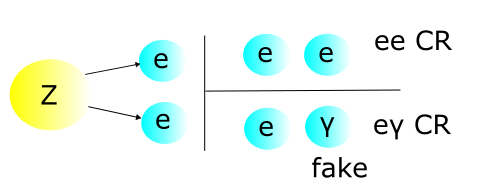
\includegraphics[width=0.69\textwidth]{figures/efake_CRs.png}}
\caption [] {Graphical representation of the $ee$ and $e\gamma$ control regions.}
\label{fig:egammafake_cr_toy}
\end{figure} 


\subsection{Control regions}
\label{sec:egammafakes_cr}

To study the $e\to\gamma$ fake rate, a fake enriched control region is defined by selecting events having a pair of back-to-back electron and photon, which will be called $e\gamma$ control region. The requirements include:
\begin{itemize}
\item Exactly one electron which is trigger matched.
\item At least one photon. The leading \pt photon is referred simply as photon in the following.
\item The opening angle between the electron and the photon to be larger than 150 degrees. This requirement helps to reduce different backgrounds due to hadron being misreconstructed as photon and prompt photons radiated from the electron.
\item The invariant mass of the electron and the photon to be within 50 GeV around the $Z$ mass. 
\end{itemize}
In the selected events, the electron is called \textit{tag electron} and the photon is called \textit{probe photon}.

Another control region, that will be called $ee$ control region, is defined in exactly the same way as above, but by replacing the photon in the requirements with an electron which should have opposite charge sign with respect to the tag electron. Thus, this electron is called \textit{probe electron} and is used as a reference to be compared with the probe photon to define the fake rate later. Complete definition of the $ee$ and $e\gamma$ control regions is shown in the Figure~\ref{fig:egammafake_cr}.

\begin{figure}[!htbp]
\centering
%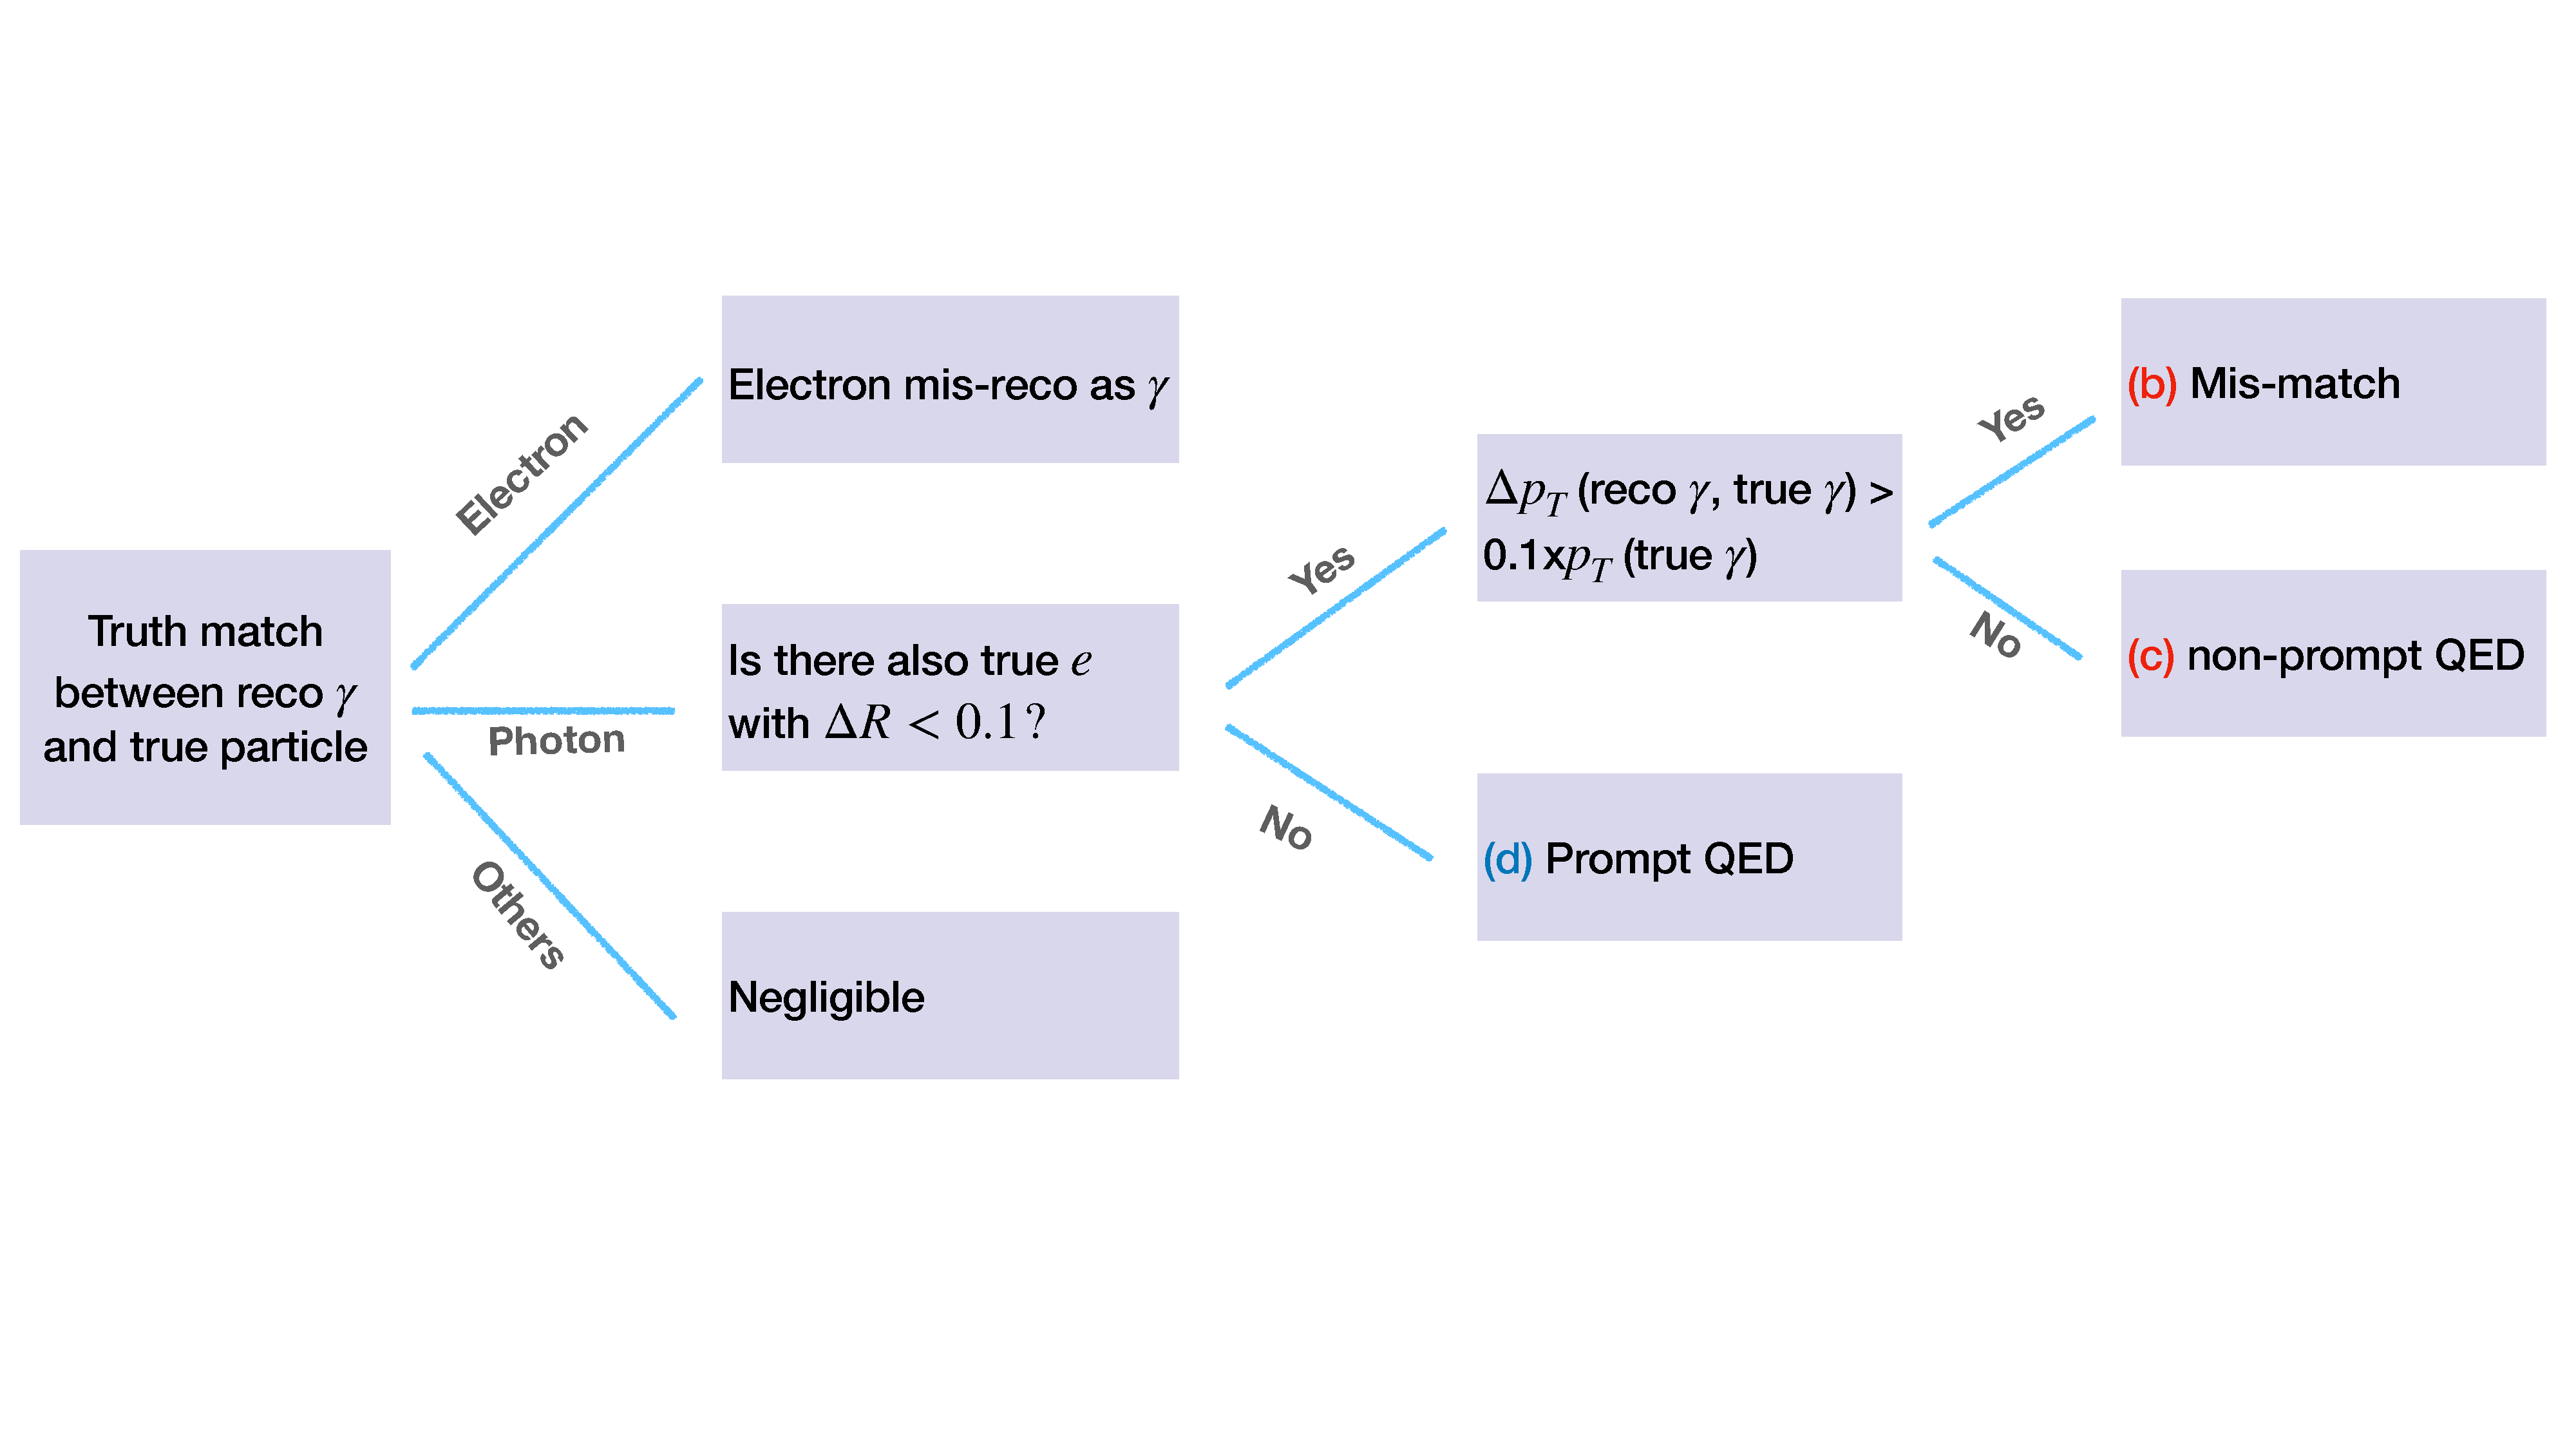
\includegraphics[width=0.49, scale=2.0\textwidth]{figures/egammafakes/efake_truth_matching.pdf}}
{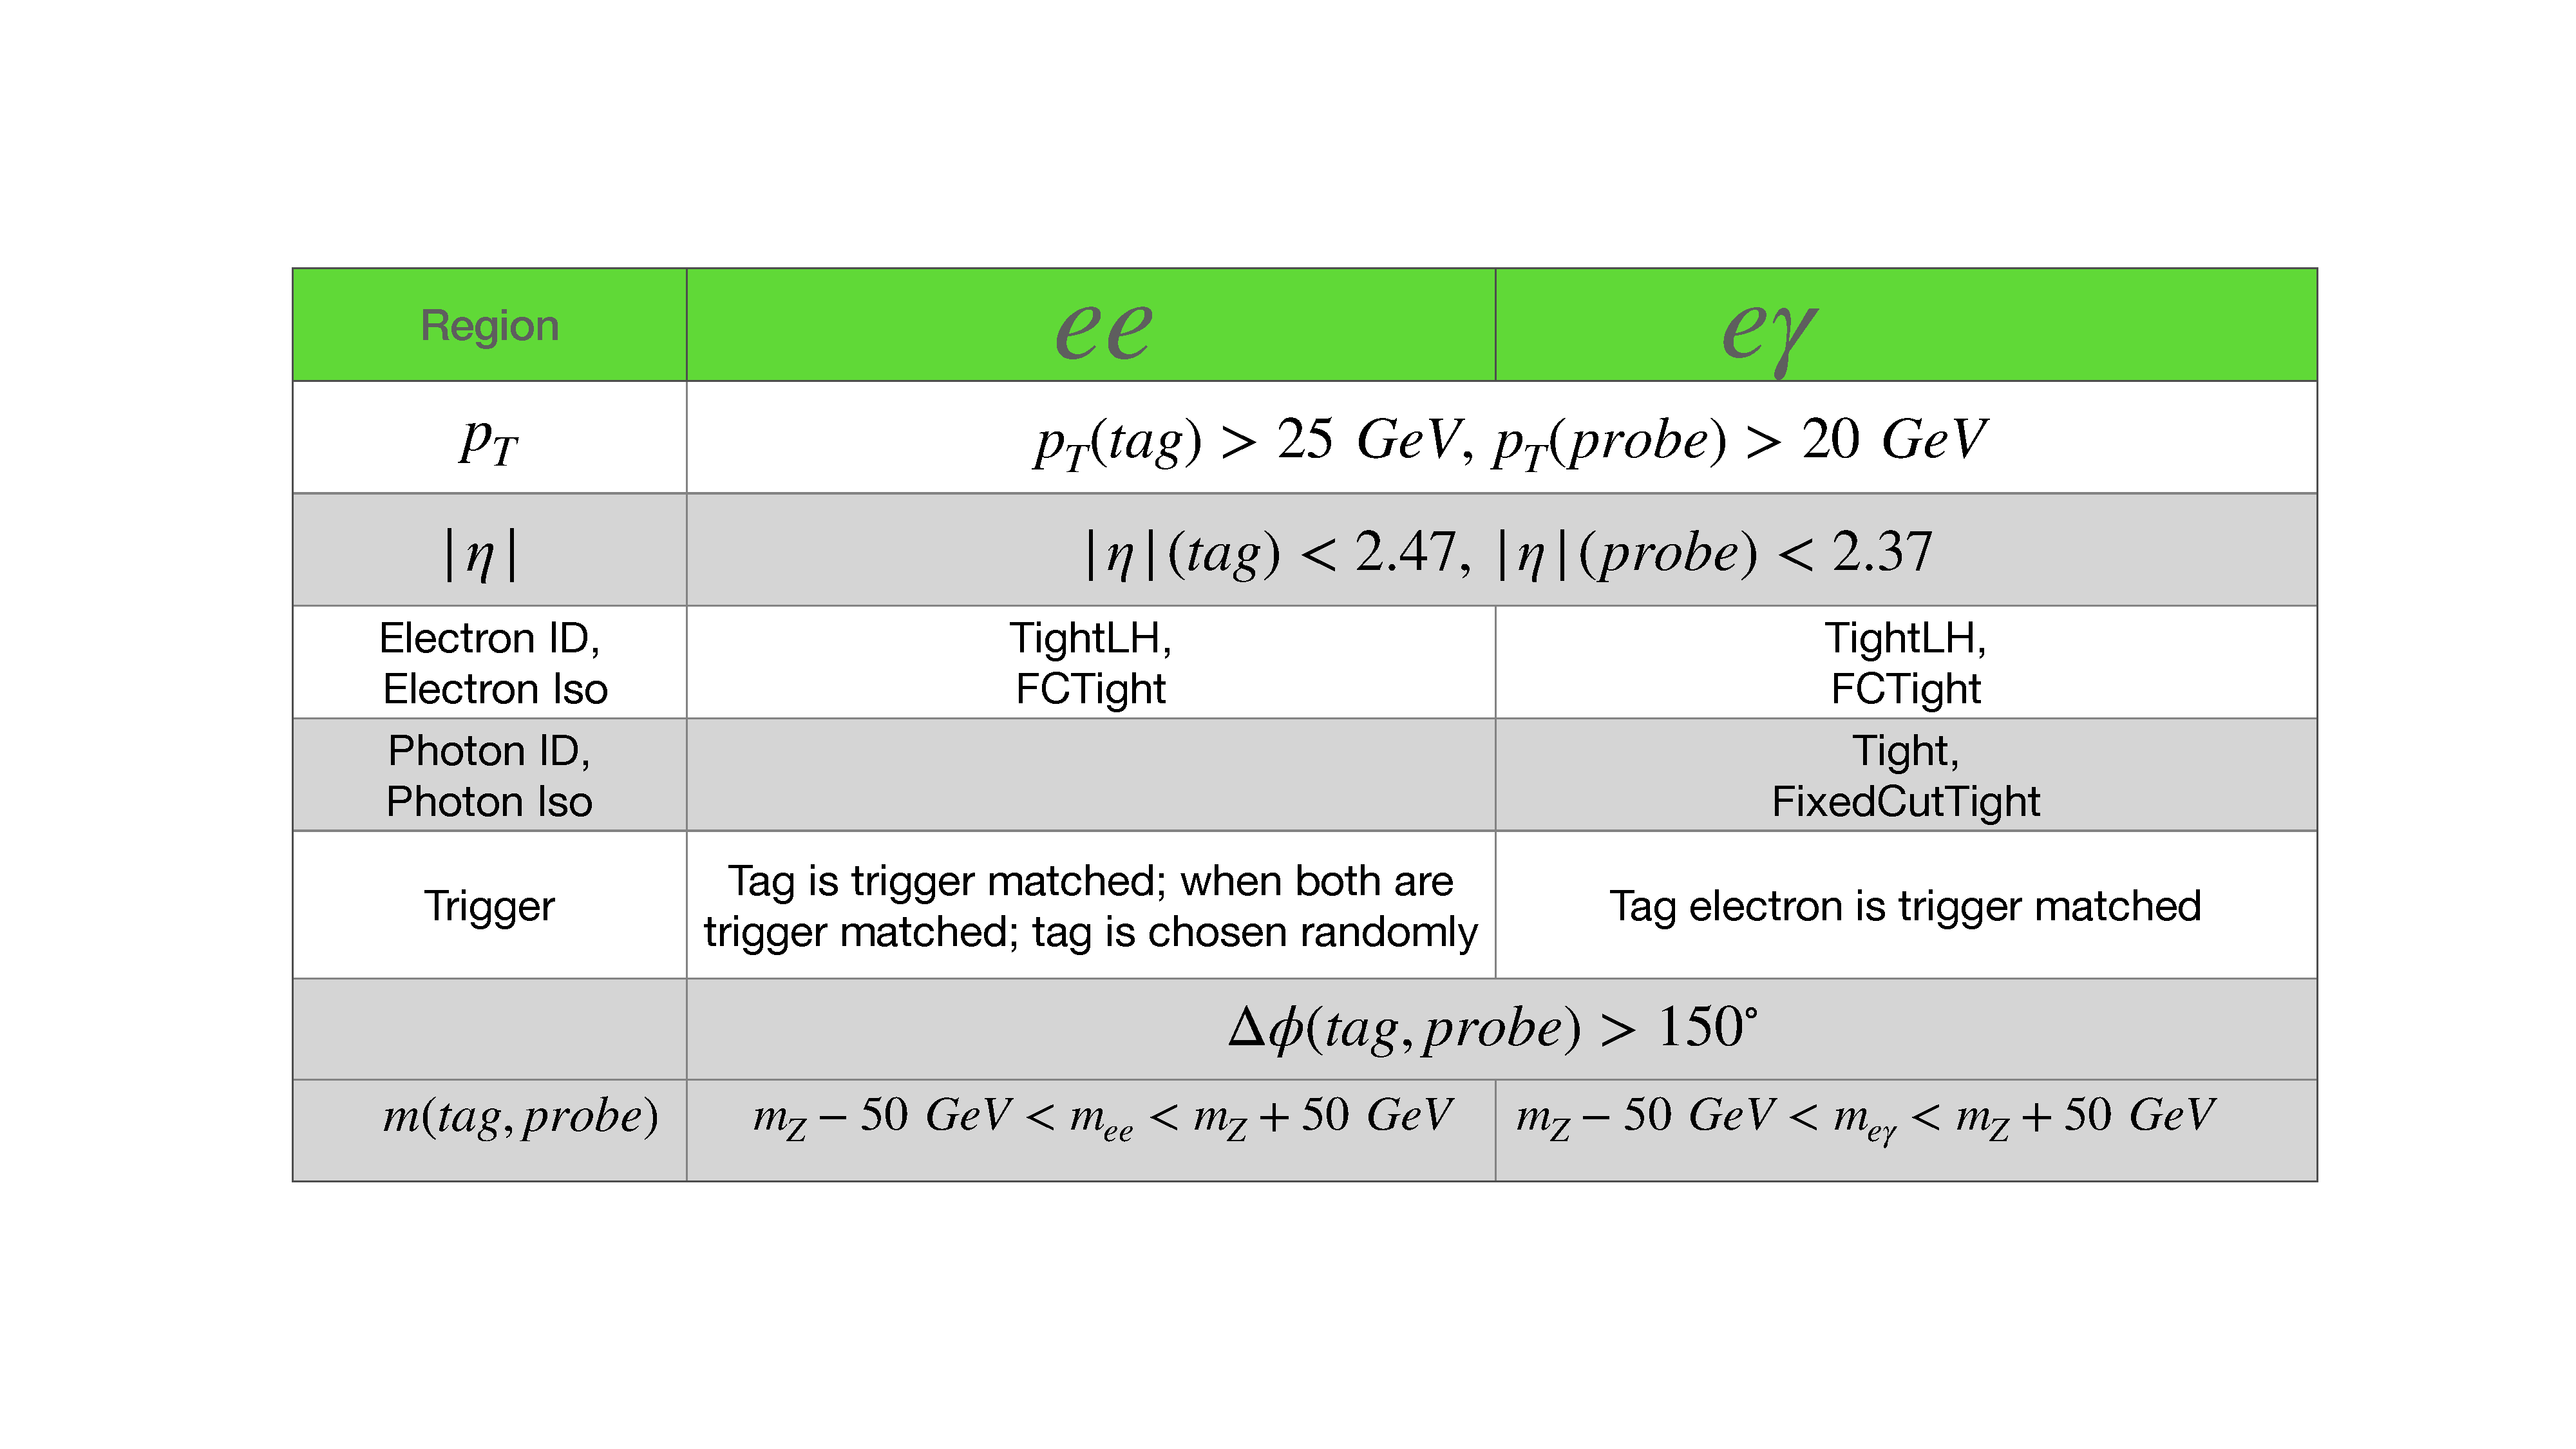
\includegraphics[width=0.69\textwidth]{figures/egammafakes/efakeCR.pdf}}
\caption [] {Definition of $ee$ and $e\gamma$ control regions.}
\label{fig:egammafake_cr}
\end{figure} 

%The cut-flows of these two control region selections are shown in Table~\ref{tab:egammafake_crcutflow} in Appendix~\ref{app:cutflow} for the $Z\to ee$ MC sample, which is expected to be the dominant process in these two control regions.

\FloatBarrier
\subsection{Fake sources}
\label{sec:egammafakes_source}

The $Z\to ee$ MC events selected in the above described $e\gamma$ control region can be used to study the source of $e\to\gamma$ fakes, by matching the probe photon with a truth particle before the detector simulation.
The matching is done by extrapolating the track of the truth particle to the calorimeter layer and calculating the angular distance between the truth particle and the EM cluster, from which the photon is reconstructed.
If the distance is smaller than a reference value ($\Delta R < 0.3$), the truth particle is considered to be the source of the photon.

After truth matching, the photon is categorised into four classes.
\begin{itemize}
\item Type (a): denoted as "mis-reco.", where the photon is matched to a true electron. 87\% of the selected photons belong to this class.
\item Type (b): denoted as "mis-match", where the photon is matched to a true photon, but the photon's \pt is larger than that of the true photon by more than 10\%\footnote{The 10\% threshold is chosen such that it is larger than the photon \pt resolution, of the order of a few percent, and thus such a large difference are expected to arise from a mismatch about the objects.}, and at the same time, there is a nearby true electron with $\Delta R < 0.1$ w.r.t. the photon. 
1.8\% of the selected photons belong to this class.
\item Type (c): denoted as "non-prompt QED", where the photon is matched to a true photon, and their relative \pt difference is smaller than 10\%, although there is a nearby true electron with $\Delta R < 0.1$ w.r.t. the probe photon. 3\% of the selected photons belong to this class. The categorization into type (b) and (c) using the 10\% criterion is only done for illustration purposes to better understand the composition of the fake photons. All three categories (a) -- (c) are considered inclusively as $e\rightarrow \gamma$ fakes. %This categorization is done only for illustration of the impact of different sources.

\item Type (d): denoted as "prompt QED", where the photon is matched to a true photon, and there is no nearby true electron with $\Delta R < 0.1$ w.r.t. the photon. 
8\% of the selected photons belong to this class. 
\end{itemize}
The categorization is summarized in Figure~\ref{fig:egammafake_classes}. The categorization is meant for illustration purposes, all sources of $e\rightarrow \gamma$ fake photons (type(a), type(b) and type(c)) are considered to estimate the fake rate in MC. 


\begin{figure}[!htbp]
\centering
%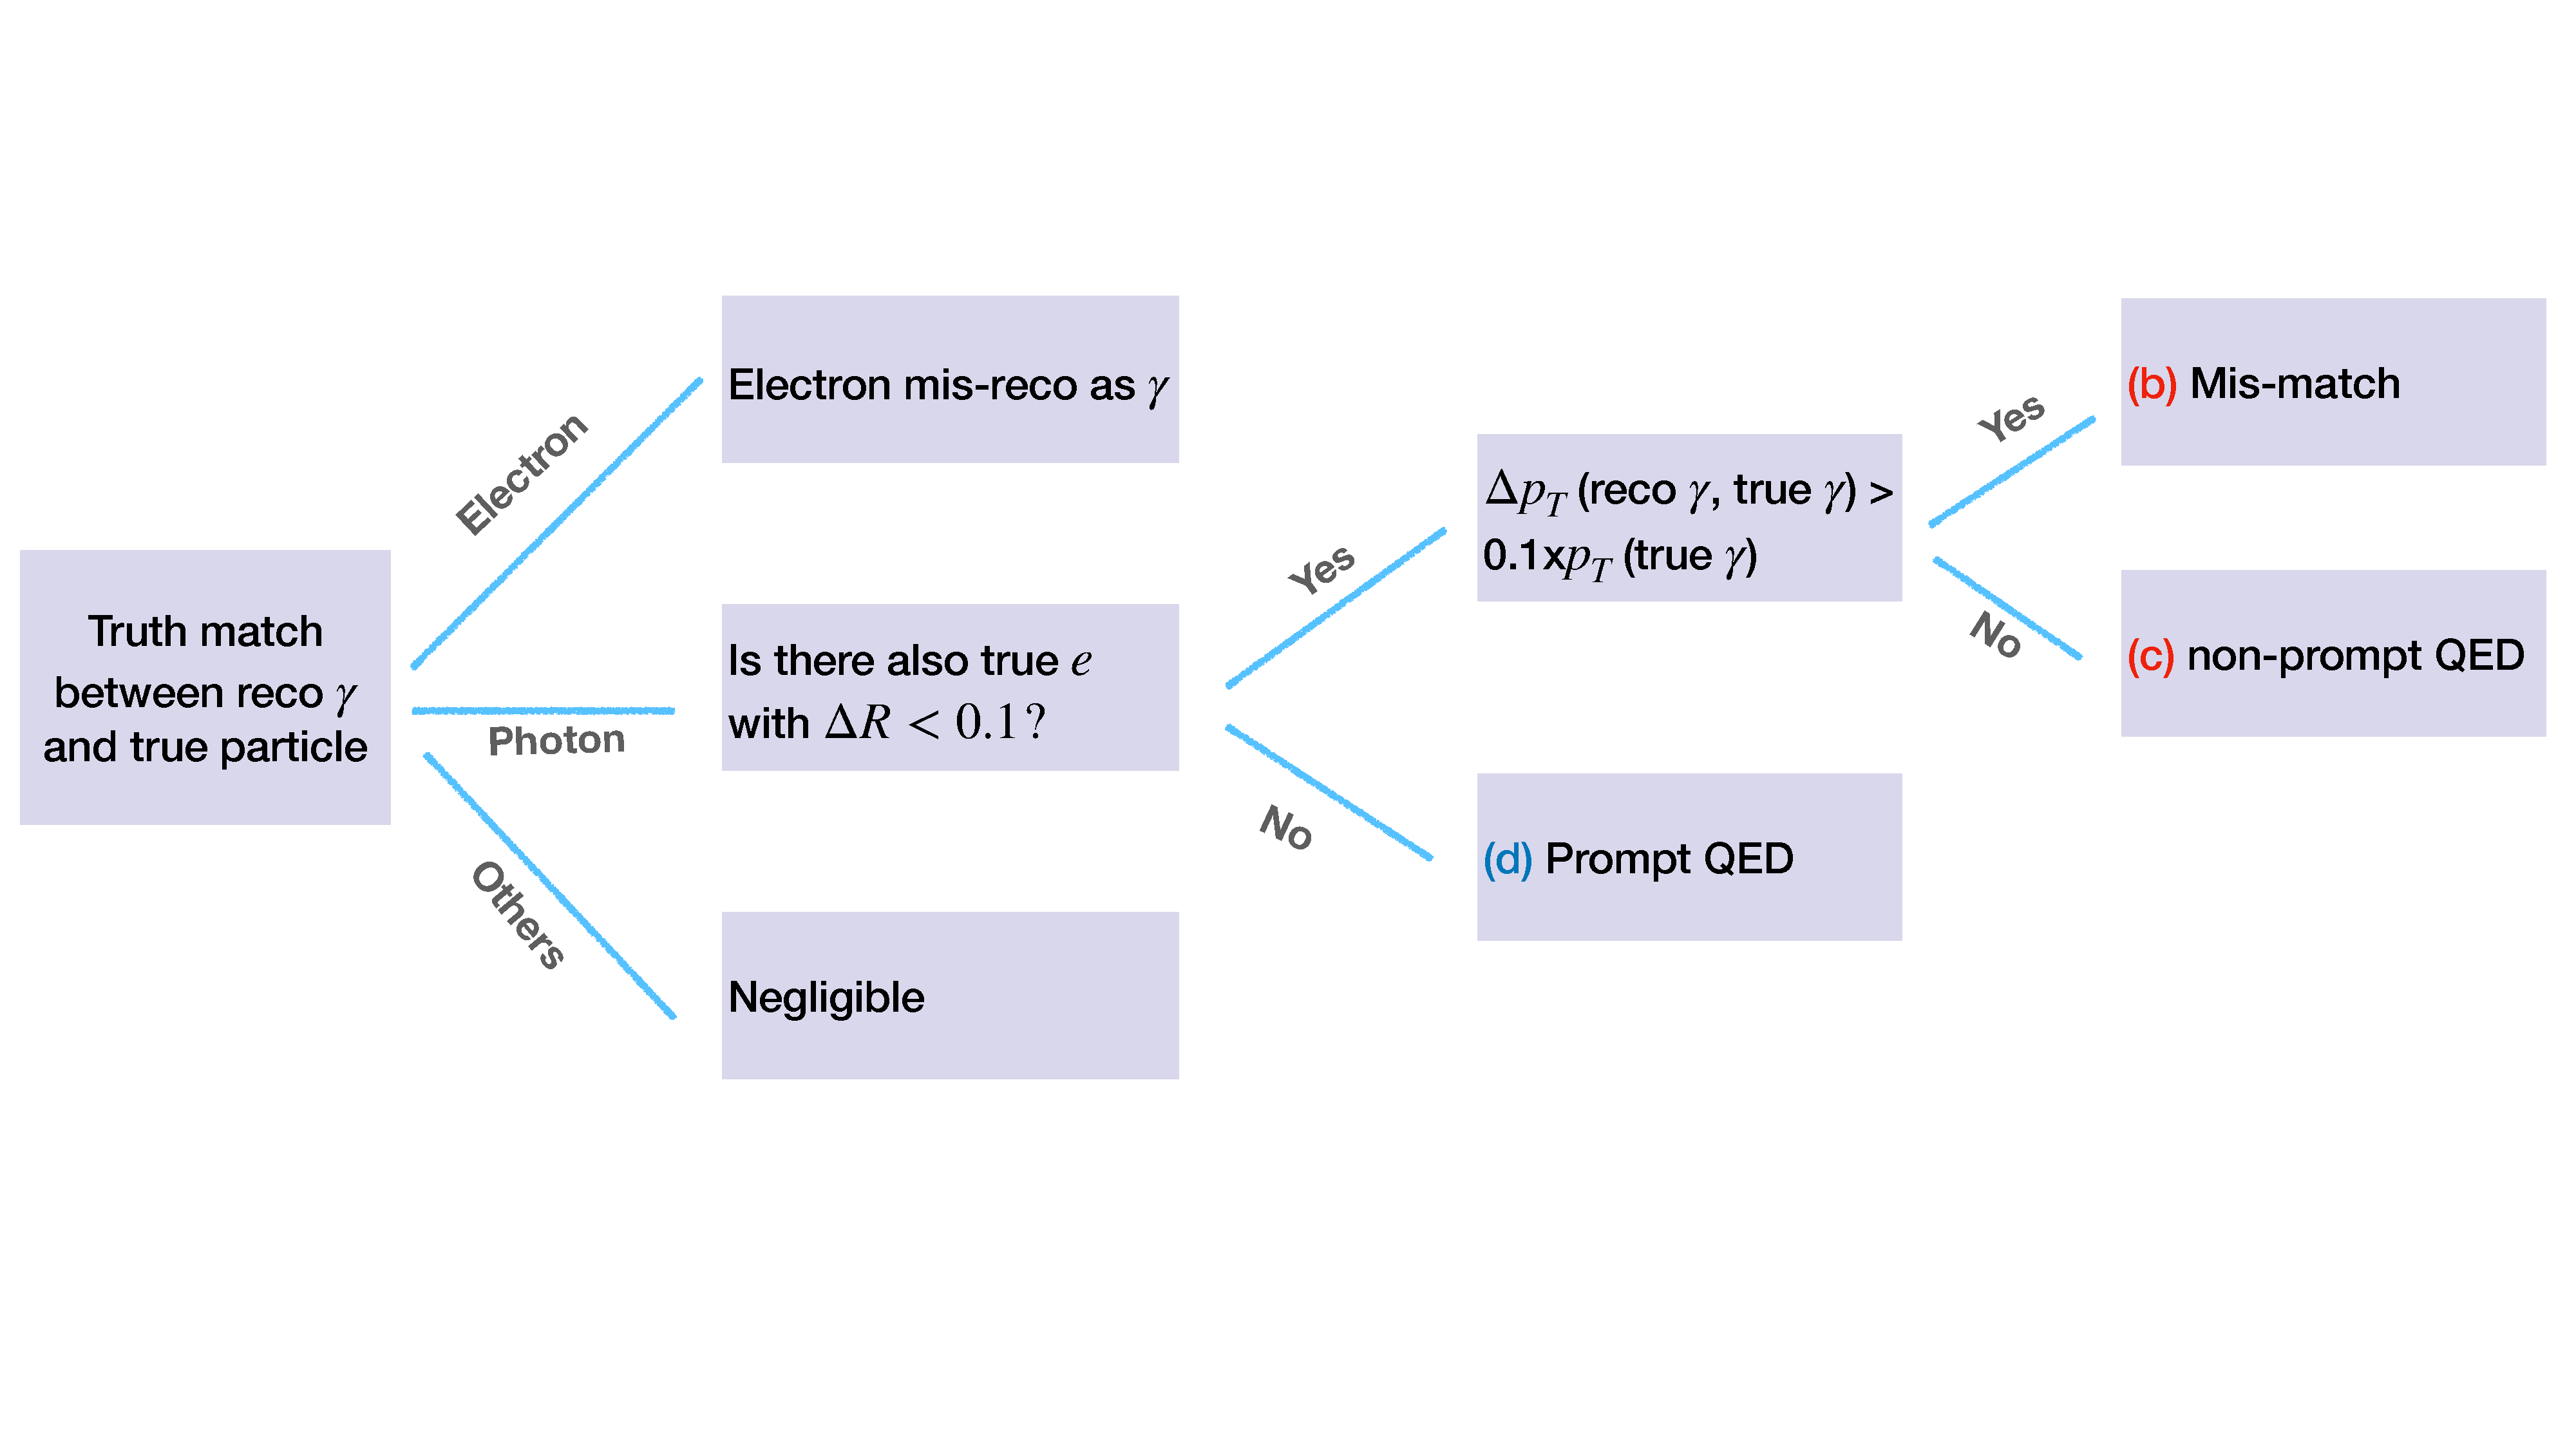
\includegraphics[width=0.49, scale=2.0\textwidth]{figures/egammafakes/efake_truth_matching.pdf}}
{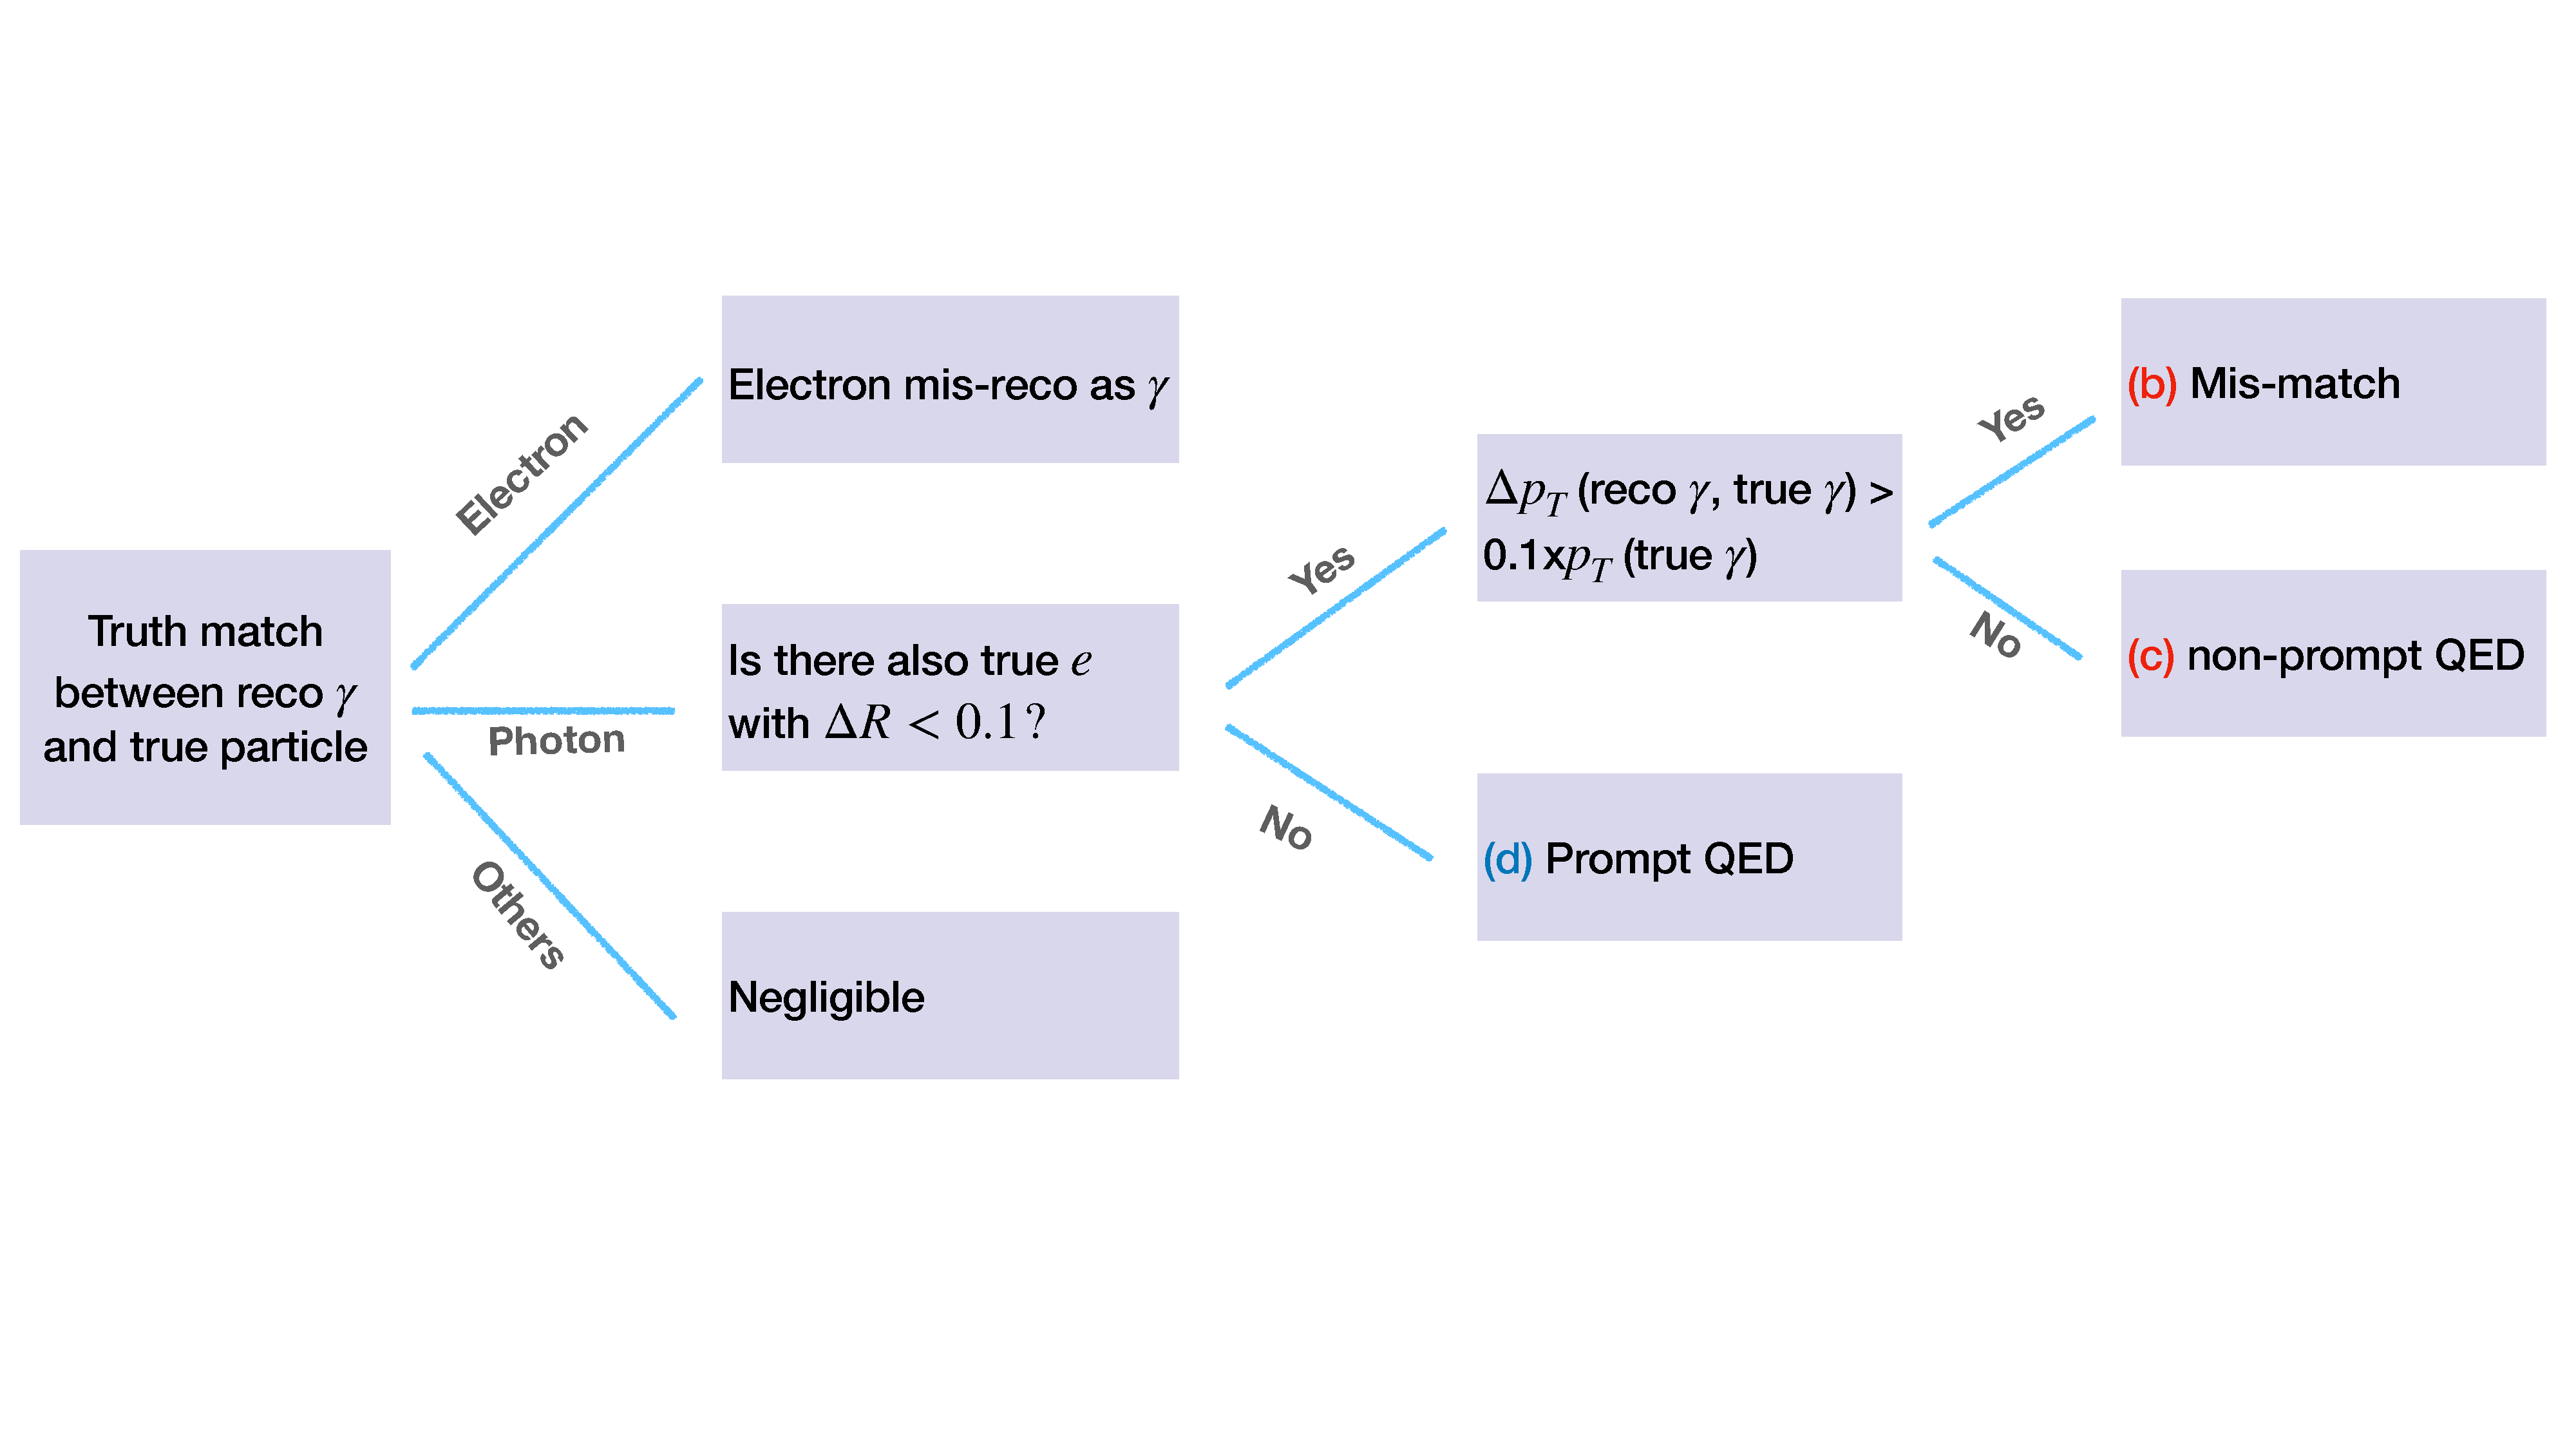
\includegraphics[width=0.69\textwidth]{figures/egammafakes/efake_truth_matching.pdf}}
\caption [] {The categorisation of the selected probe photons in the $e\gamma$ control region via truth particle matching.}
\label{fig:egammafake_classes}
\end{figure}  

In the following, to better understand these four types of photons, their kinematics are shown and compared to that of the probe electron, when available.

The \pt and $\eta$ of the probe photons are compared to those of the probe electron in Figure~\ref{fig:egammafake_probepteta}. 
It can be seen that the \pt spectrum is rather similar between photon type (a), (b), and (c) and the probe electron, which indicates that they are truly $e\to\gamma$ fakes.
For the $\eta$ distribution, type (a) and (b) peak at high $\eta$ region. Connecting to the fact that there is also larger upstream material in high $\eta$ region, it implies (a) and (b) are likely to be bremsstrahlung photons.
For type (c), its $\eta$ spectrum is very similar to that of the probe electron. This could be explained by a very hard non-prompt QED that takes away almost all kinematics of its mother electron.

The invariant mass between the tag and probe in the two control regions are compared in Figure~\ref{fig:egammafake_tagmass}~\subref{fig:efakeInvmassComp}. The lower-shifted mass spectrum for type (d) indicates that it is a true prompt photon from the three body decay of $Z\to e^+e^- +\gamma$. Therefore, type (d) is not to be counted as $e\rightarrow \gamma$ fake. The invariant mass distribution of tag electron and probe photon is shown in Figure~\ref{fig:egammafake_tagmass}~\subref{fig:efakeInvmassStack}, with each type of photons being normalized to their expected yields. It can be seen that the fake is dominated by the type (a).


\begin{figure}[!htbp]
\centering
\subfloat[]{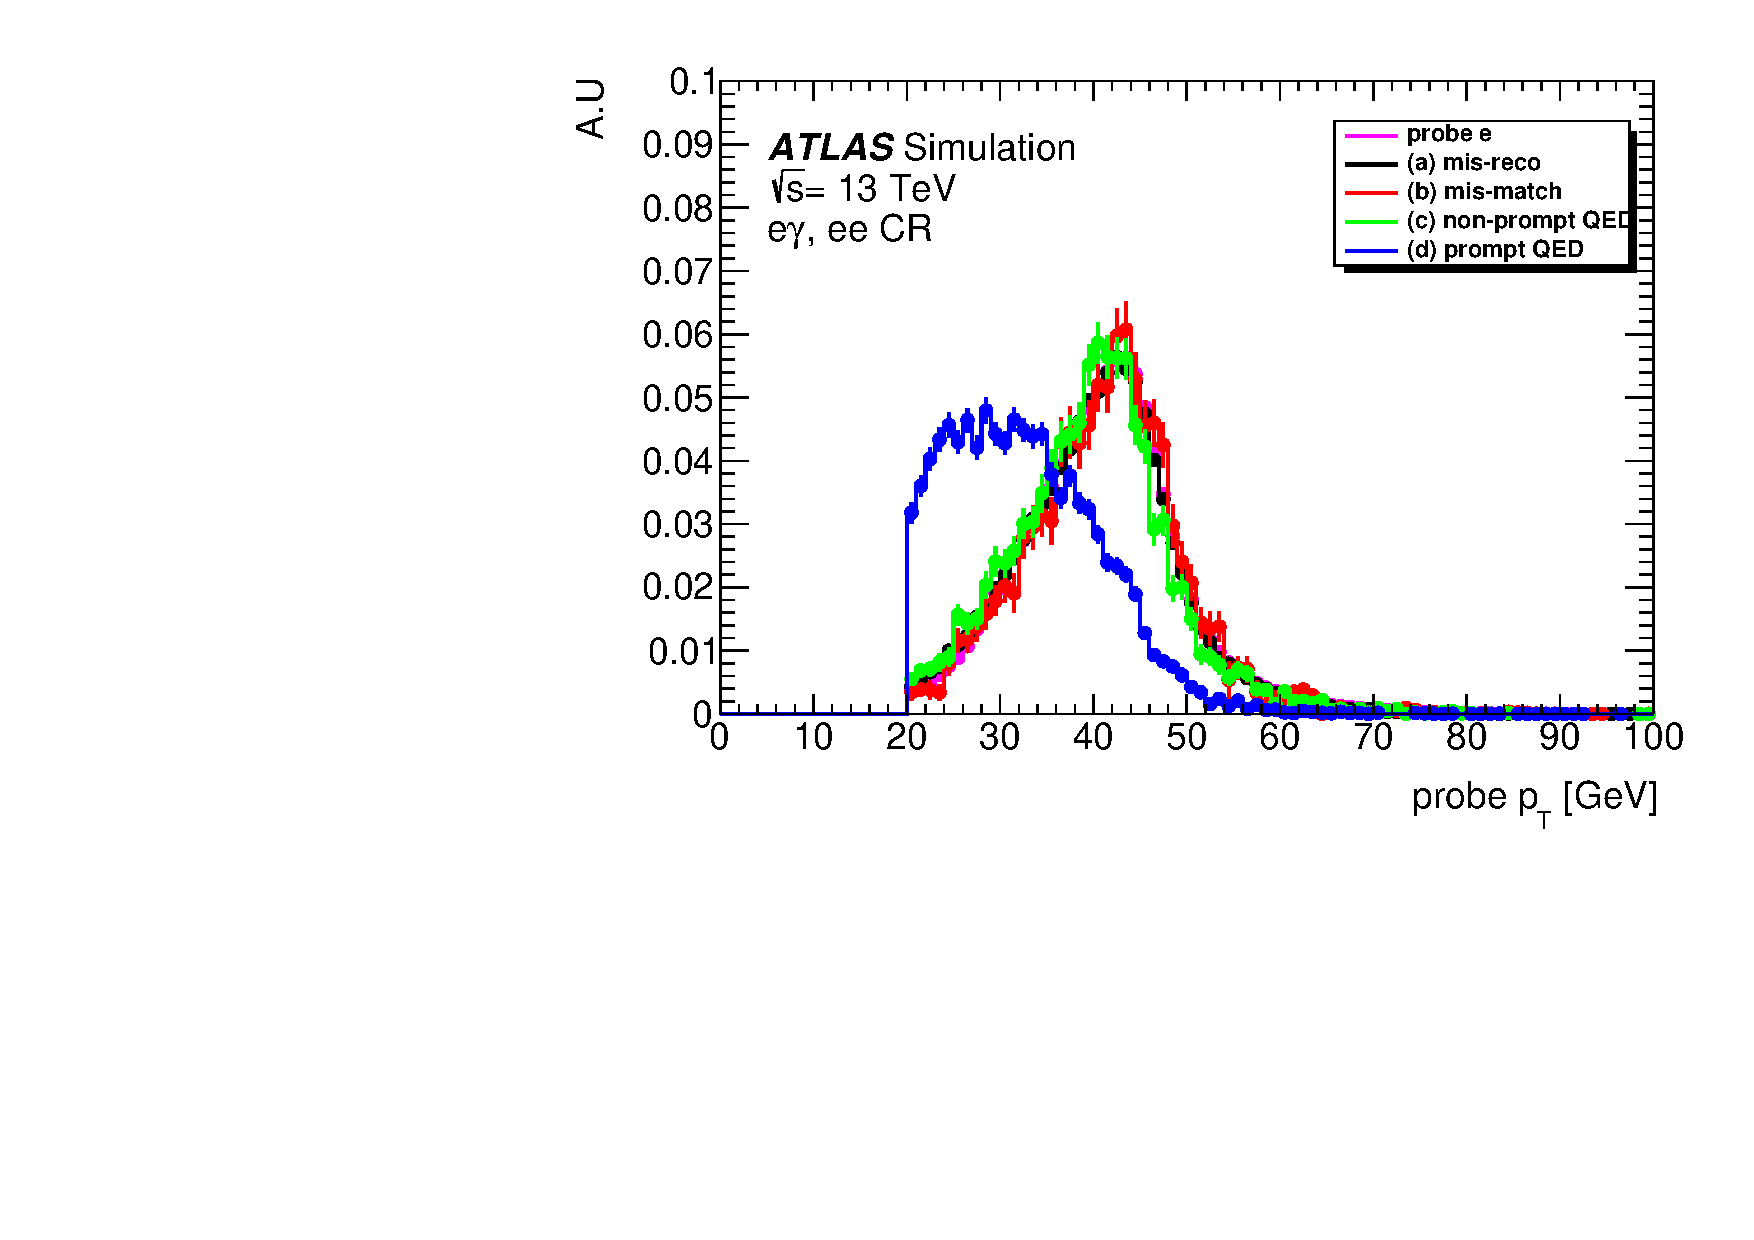
\includegraphics[width=0.49\textwidth]{figures/egammafakes/probe_efake_pt.pdf}}
\subfloat[]{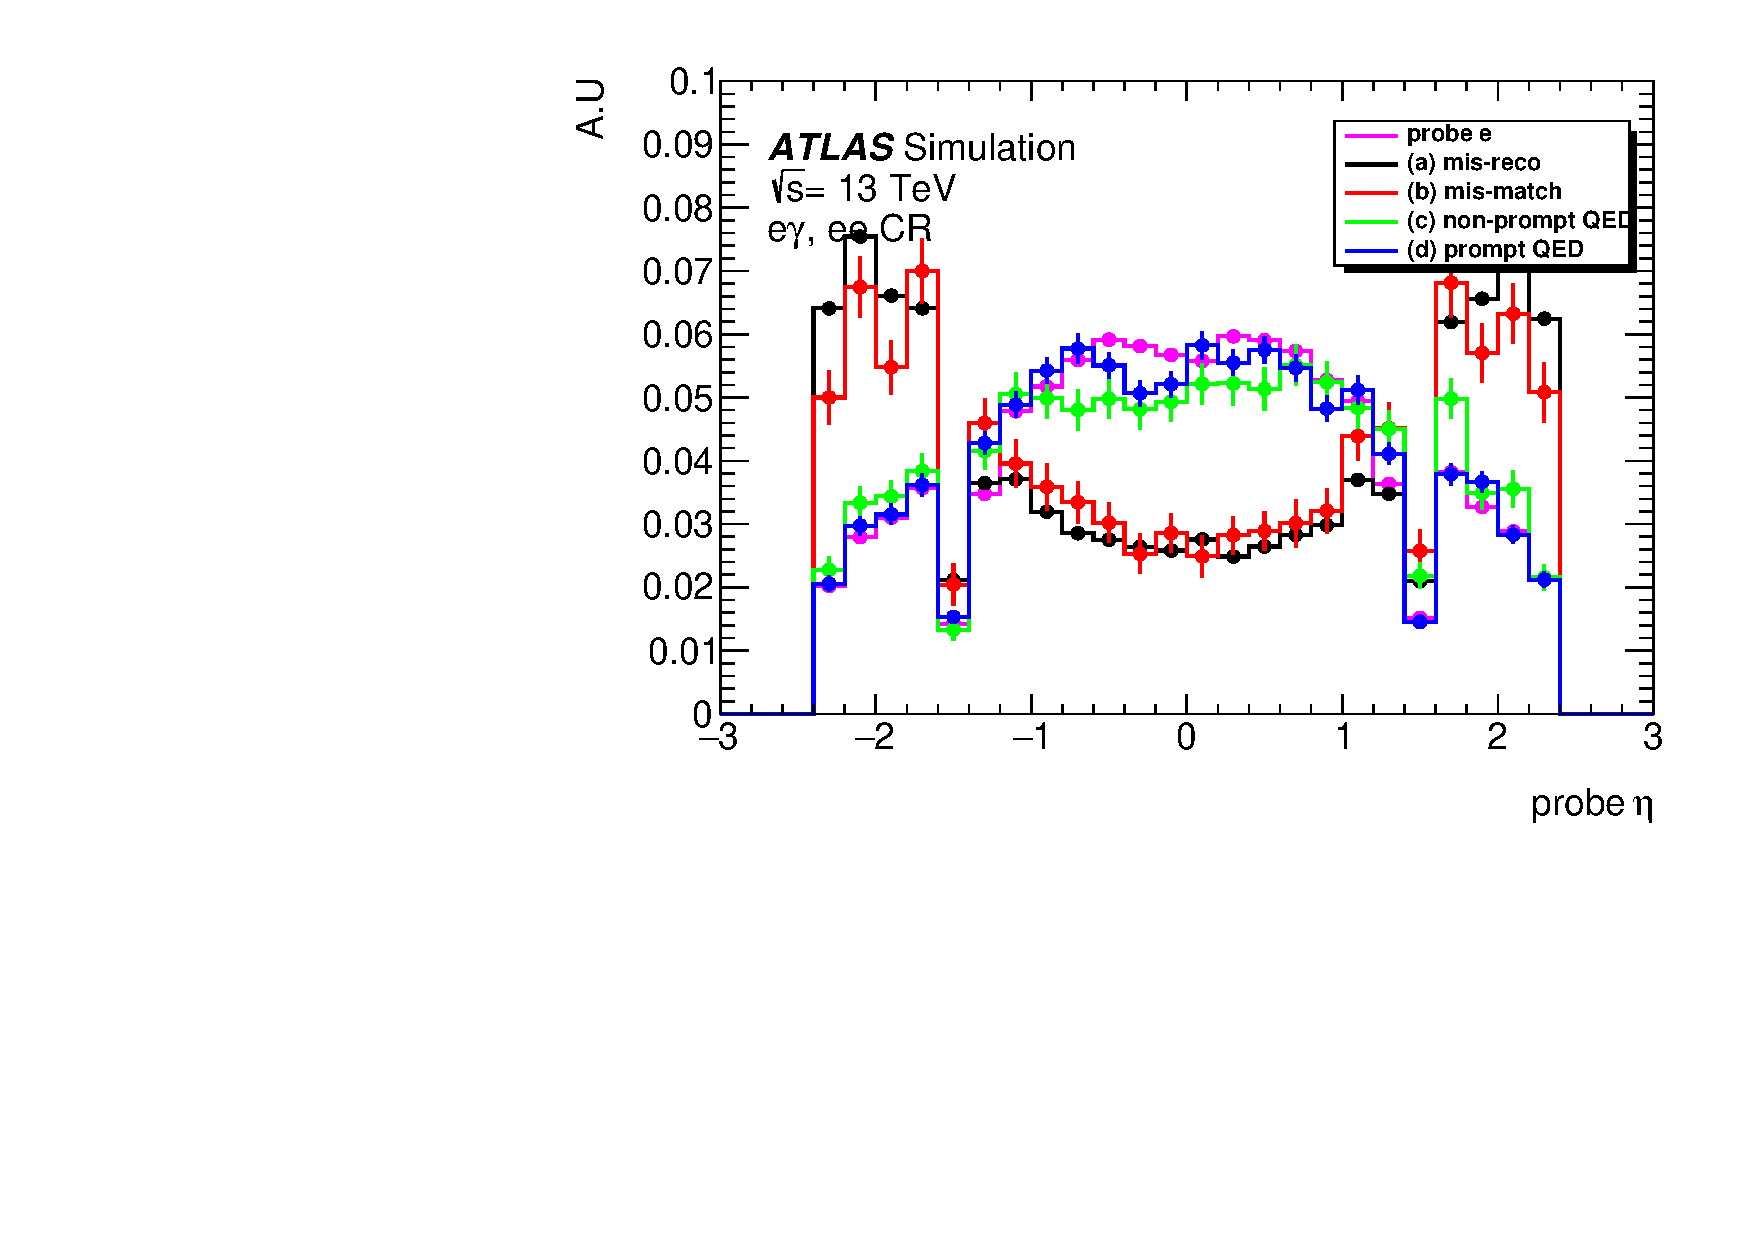
\includegraphics[width=0.49\textwidth]{figures/egammafakes/probe_efake_eta.pdf}}
	\caption [] {The \pt (a) and $\eta$ (b) distributions of different types of probe photon in the $e\gamma$ CRs. The distributions are compared with the kinematic properties of the probe electron in the $ee$ CR. The distributions are obtained using $Z\rightarrow e^+e^-$ MC. In the $e\gamma$ CR most of the photons correspond to a misreconstructed electron. In that case, if the photon in the $e\gamma$ CR corresponds to a misreconstructed electron, then it should have similar kinematic distribution as the probe electron in the $ee$ CR.}
\label{fig:egammafake_probepteta}
\end{figure}   

\begin{figure}[!htbp]
\centering
\subfloat[]{
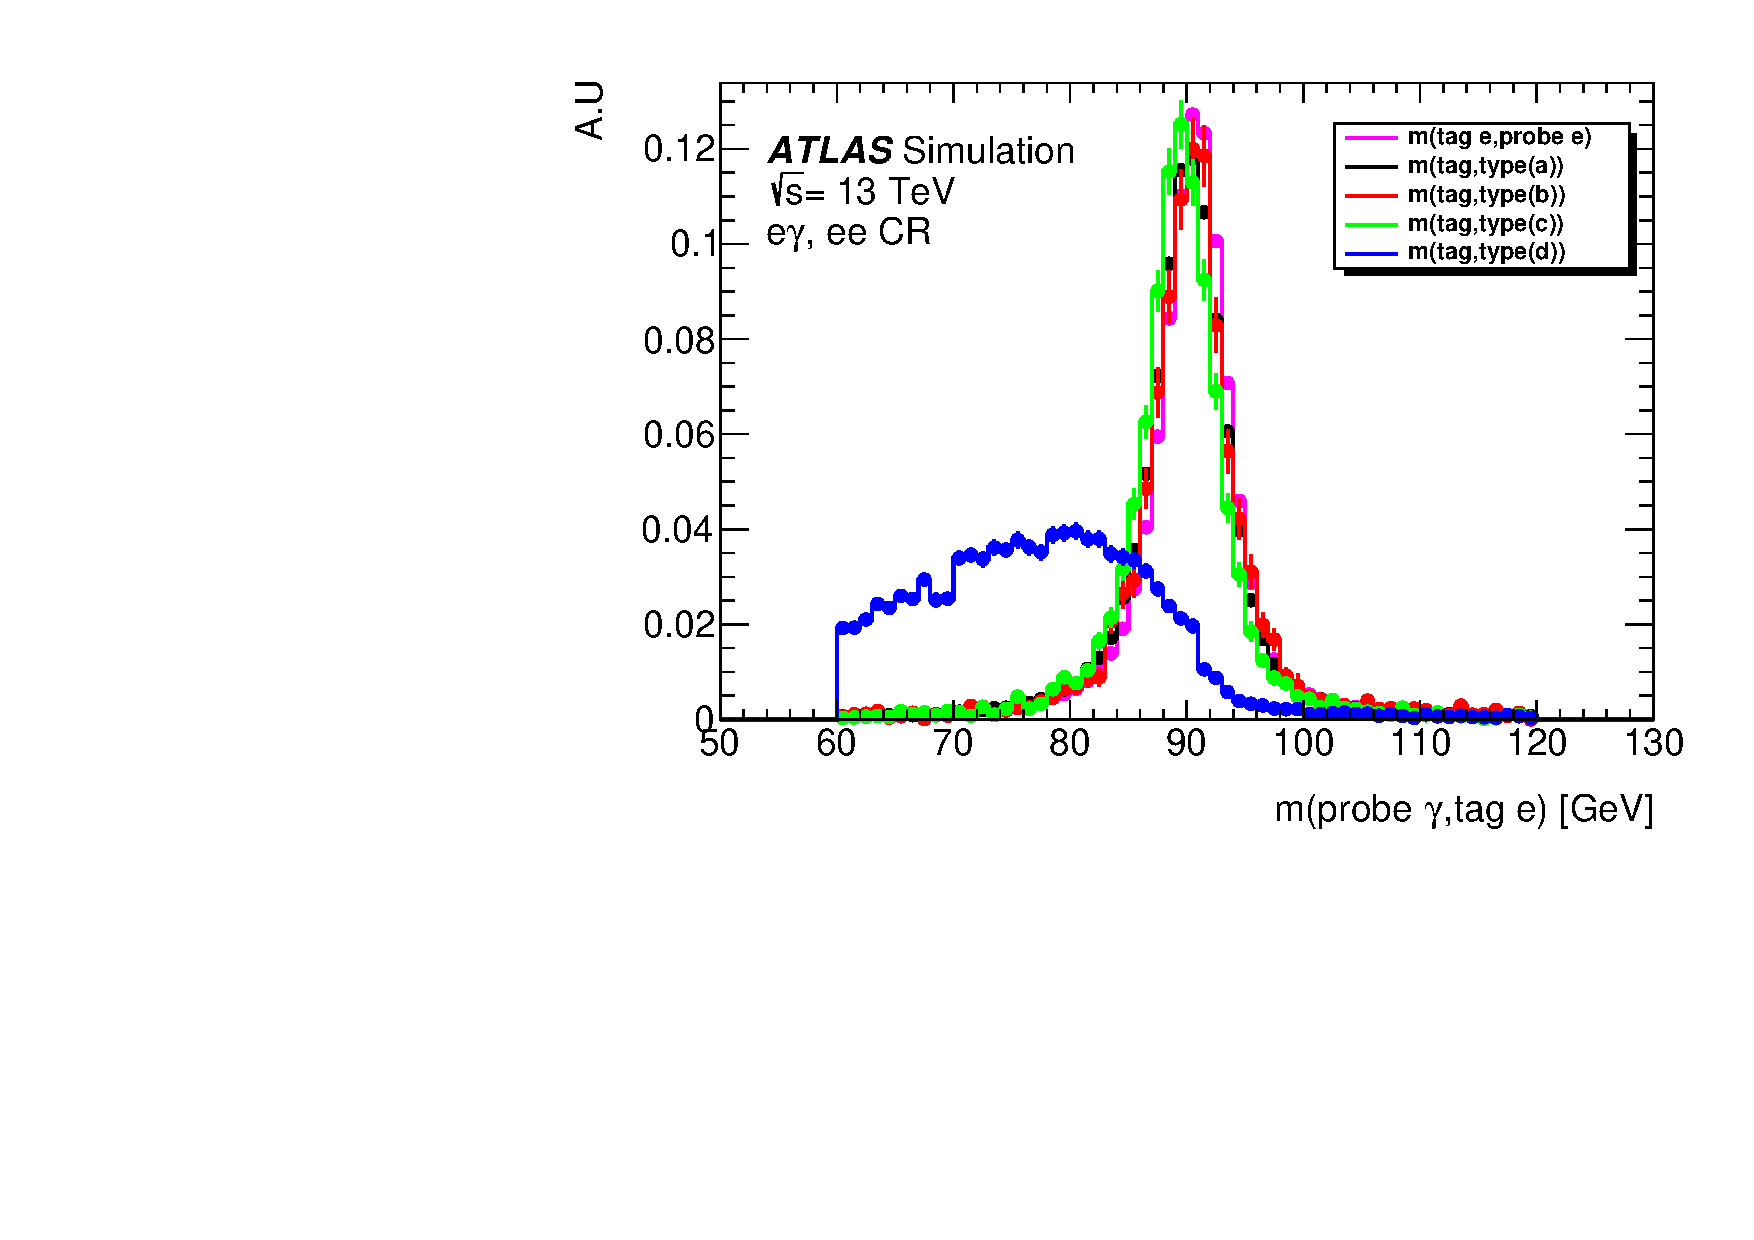
\includegraphics[width=0.49\textwidth]{figures/egammafakes/efake_invmass_comp.pdf}\label{fig:efakeInvmassComp}
}
\subfloat[]{
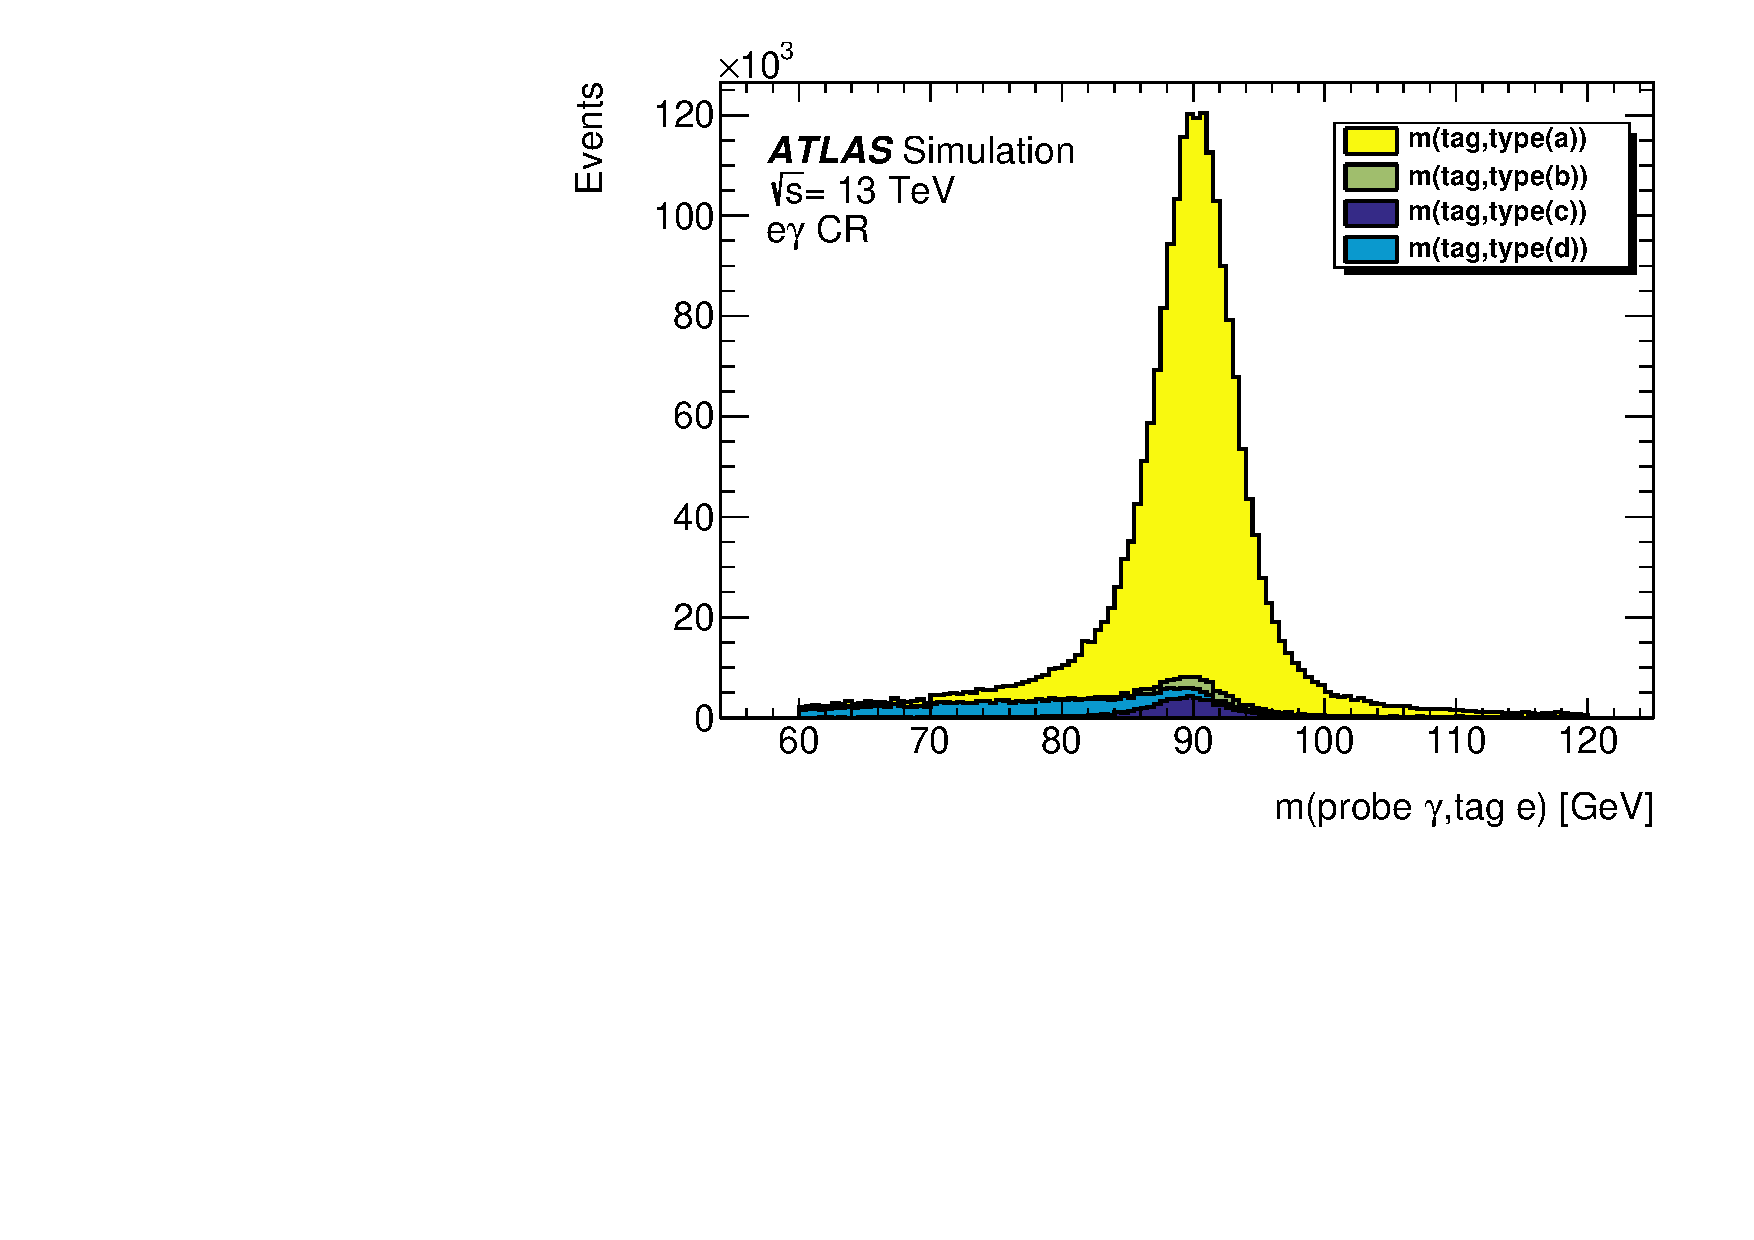
\includegraphics[width=0.49\textwidth]{figures/egammafakes/efake_invmass_stack.pdf}\label{fig:efakeInvmassStack}
}
\caption [] {(a) Normalized invariant mass distribution between the tag and different probe types in the $e\gamma$ and $ee$ CR.(b) The invariant mass between the tag and different probe types in $e\gamma$ CR.}
\label{fig:egammafake_tagmass}
\end{figure} 
  

\FloatBarrier
\subsection{Fake rates}
\label{sec:egammafakes_fr}

Using the $Z\to ee$ MC, the number of $Z\to ee$ events observed with a tag electron in any place and a fake photon in a particular bin can be expressed as follows:
\begin{equation}
N_{e,\gamma}^i = N_{true}^i \times \epsilon_e^{reco} \times \epsilon_e^{\mathrm{others}} \times p_{e\to\gamma}^i \times \epsilon_{\gamma(F)}^i
\end{equation}
where
\begin{itemize}
\item $i$ is the binning index of \pT or $\eta$ or both
\item $N_{true}^i$: true number of generated $Z\to ee$ events where the probe electron is in bin $i$
\item $\epsilon_e^{reco}$ and $\epsilon_e^{\mathrm{others}}$: reconstruction and other selection efficiencies of tag electron
\item $p_{e\to\gamma}^i$: probability of misidentifying an electron as photon in bin $i$
\item $\epsilon_{\gamma}^i(F)$: selection efficiency of the fake photon in bin $i$ ("F" denotes the fact that it's a fake photon so that the efficiency can be different from the true photon)
\end{itemize}

Also, the number of $Z\to ee$ events observed with a tag electron in any place and a probe electron in a particular bin can be expressed as follows:
\begin{equation}
N_{e,e}^i = N_{true}^i \times \epsilon_{e1}^{reco} \times \epsilon_{e1}^{\mathrm{others}} \times \epsilon_{e2}^{reco,i} \times \epsilon_{e2}^{\mathrm{others},i}
\end{equation}
where
\begin{itemize}
\item $\epsilon_{e1}^{reco}$ and $\epsilon_{e1}^{\mathrm{others}}$: reconstruction and other selection efficiencies of tag electron
\item $\epsilon_{e2}^{reco,i}$ and $\epsilon_{e2}^{\mathrm{others},i}$: reconstruction and other selection efficiencies of probe electron in bin $i$
\end{itemize}

The fake rate (FR) in a particular bin $i$ is then defined as the ratio between $N_{e,\gamma}^i$ and $N_{e,e}^i$:
\begin{equation}
\text{FR}^i \equiv \frac{N_{e,\gamma}^i}{N_{e,e}^i} = p_{e\to\gamma}^i \times \frac{\epsilon_{\gamma}^i(F)}{\epsilon_{e2}^{reco,i} \cdot \epsilon_{e2}^{\mathrm{others},i}} = p_{e\to\gamma}^i \times C^i
\end{equation}
From the above formula, it is known that $FR^i$ is proportional to the $e\to\gamma$ faking probability in that bin. The proportion coefficient $C^i$ could also vary.
%nd $\eta$ of the fake candidate, due to the \pt and $\eta$ dependency of those efficiencies.

%An overall fake rate can be calculated using the same formula and its MC value are shown in Table~\ref{tab:egammafake_fr_mc}. 
In Figure~\ref{fig:egammafake_fr_diff}, the \pt and $\eta$ dependencies of the absolute differential fake rate are shown.  
In Figure~\ref{fig:egammafake_fr_diff}, the type (d), which is not really a $e\rightarrow \gamma$ fake photon, is shown for completeness.

%\begin{table}[h]
%\centering
%\caption[]{The overall fake rate calculated from $Z\to ee$ MC for different types of photon. Type (d) is not counted as $e\rightarrow \gamma$ fake photon and its value is just shown for completeness. Only statistical uncertainties are shown here.}
%\vspace*{0.5cm}
%\begin{tabular}{c|c|c|c}
%\hline
%\hline
%& N(probe $\gamma$) & N(probe $e$) & $\text{FR}_{\text{MC}}(\%)$ \\
%\hline
%%	Type(a) & \numRF{1903184.40}{3} $\pm$ \numRF{5493.01}{2} & \numRF{29430386.00}{3} $\pm$ \numRF{20219.12}{2} & \numRF{6.46}{2} \\ \hline 
%%	Type(b) & \numRF{38927.34}{3}   $\pm$ \numRF{754.92}{2}  & \numRF{29430386.00}{3} $\pm$ \numRF{20219.12}{2} & \numRF{0.13}{2} \\ \hline 
%%	Type(c) & \numRF{65791.93}{3}   $\pm$ \numRF{946.80}{2}  & \numRF{29430386.00}{3} $\pm$ \numRF{20219.12}{2} & \numRF{0.22}{2}\\ \hline 
%%	Type(d) & \numRF{170667.31}{3}  $\pm$ \numRF{1549.72}{2} & \numRF{29430386.00}{3} $\pm$ \numRF{20219.12}{2} & \numRF{0.58}{2} \\ \hline 
%%	All     & \numRF{2178570.98}{3} $\pm$ \numRF{5834.48}{2} & \numRF{29430386.00}{3} $\pm$ \numRF{20219.12}{2} & \numRF{7.40}{2}\\ \hline 
%\hline
%\end{tabular}
%\label{tab:egammafake_fr_mc}
%\end{table}

\begin{figure}[!htbp]
\centering
\subfloat[]{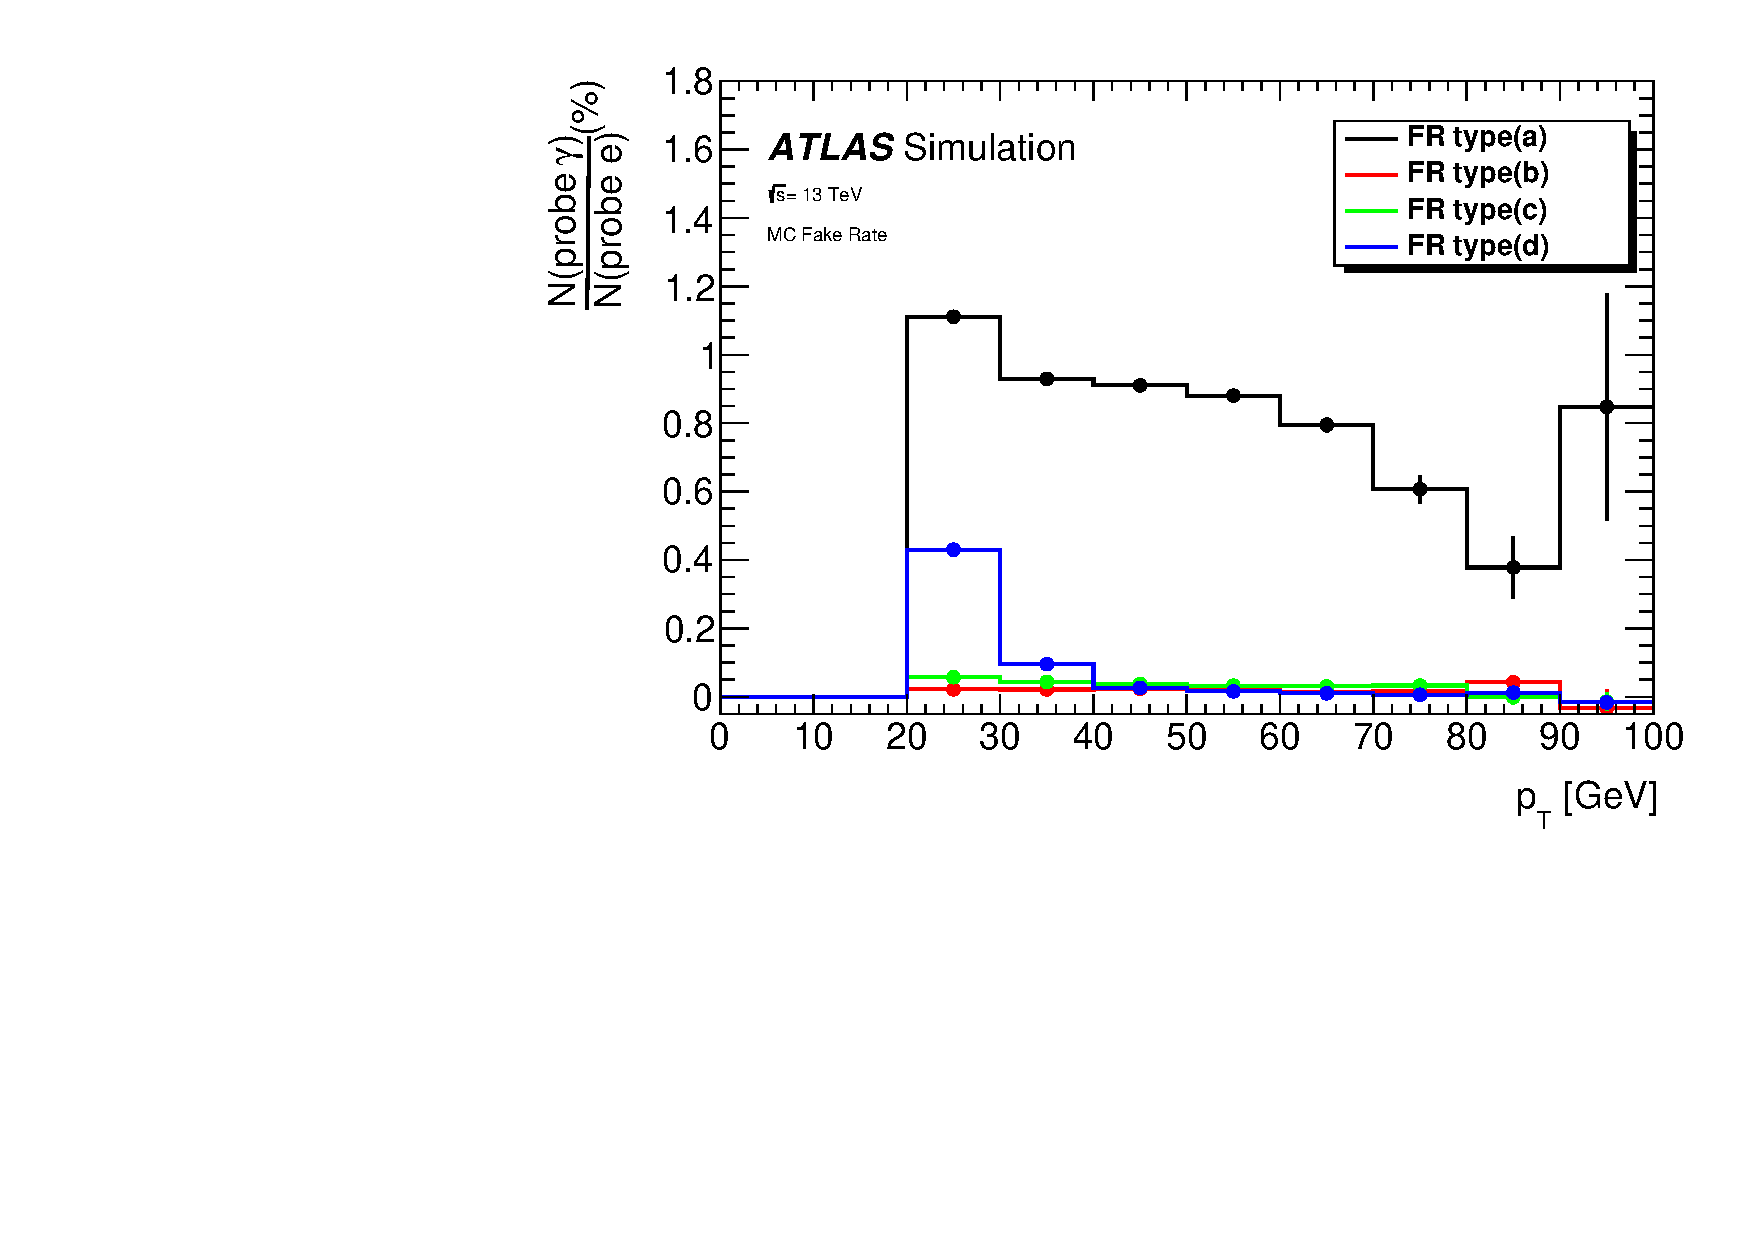
\includegraphics[width=0.49\textwidth]{figures/egammafakes/efake_rate_pt.pdf}}
\subfloat[]{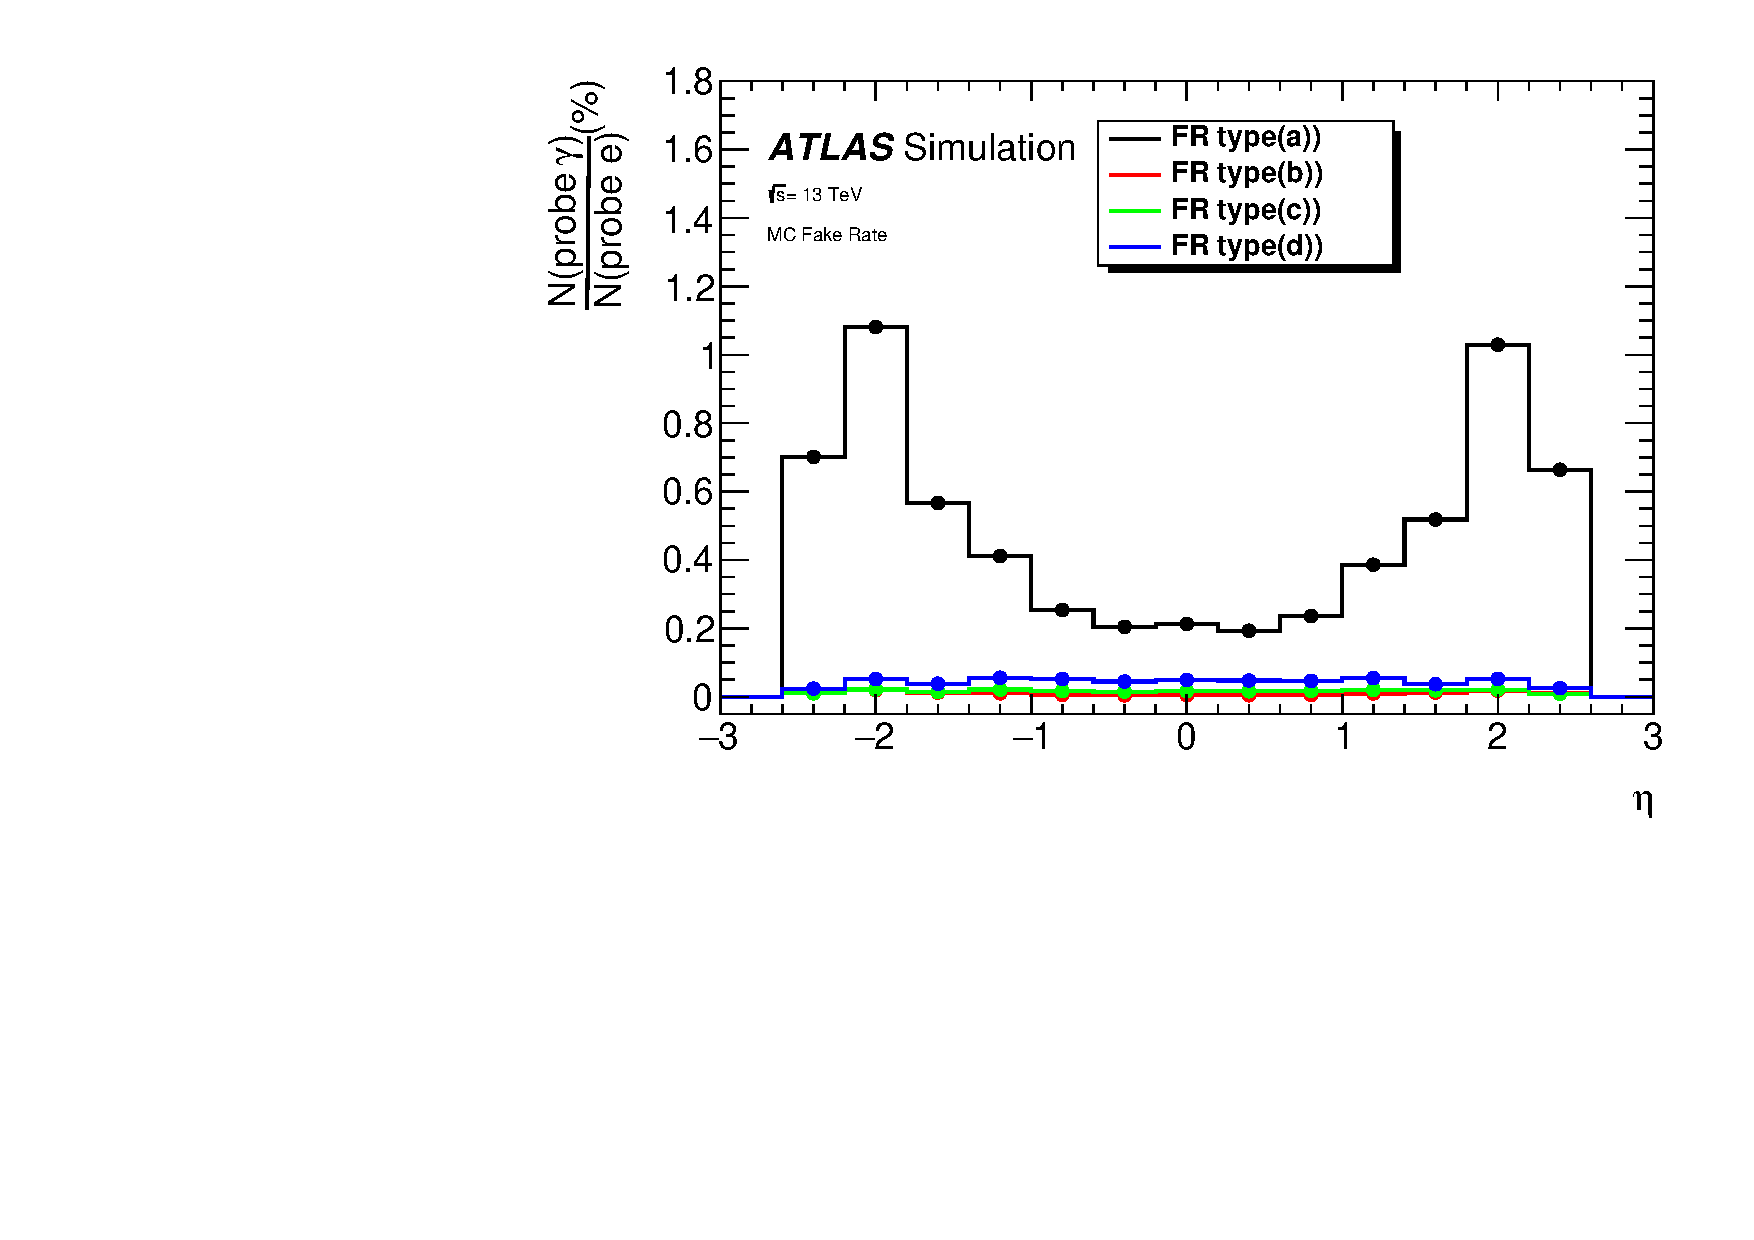
\includegraphics[width=0.49\textwidth]{figures/egammafakes/efake_rate_eta.pdf}}
\caption [] {The \pt (a) and $\eta$ (b) dependency of the fake rates}
\label{fig:egammafake_fr_diff}
\end{figure}   

In order to calculate the data-driven fake rate in bin $i$, the only difference with respect to the above MC-based fake rate is that:
\begin{equation}
\text{FR}_{dd}^i = \frac{N_{e,\gamma}^{\mathrm{data},i} - N_{e,\gamma}^{non\text{-}Z,i} - \mathrm{prompt\ QED}}{N_{e,e}^{\mathrm{data},i} - N_{e,e}^{non\text{-}Z,i} - \mathrm{prompt\ QED}}
\end{equation}
which means the denominator and numerator are replaced by their data-driven ones. 

The subtraction of non-$Z$ events from data in these control regions can't be done with MC samples since from MC study the non-$Z$ background are negligible.
Instead, it is done by side band fit,
where the $Z\to ee$ signal is modelled by double-sided Crystal-ball function and the non-$Z$ background by a Bernstein 4th order polynomial. The prompt contribution is subtracted from the data based on the MC template (type(d) photons) before the fit is performed.

After that the data-driven fake rate in bin $i$ is divided by the corresponding MC fake rate to derive a set of fake rate scale factors:
\begin{equation}
\text{SF}_{\text{FR}}^i = \frac{\text{FR}_{dd}^i}{\text{FR}_{MC}^i}
\end{equation}
these scale factors will be applied to the $e\to\gamma$ MC samples as a data-driven correction.

The scale factor is derived in photon $p_T$ and $\eta$ separately for converted and unconverted photons. It is shown in Figure~\ref{fig:egammafake_ptetadiff_sfs_conv} and Figure~\ref{fig:egammafake_ptetadiff_sfs_unconv}. The choice of binning for \pt is [25, 35, 45, 1000] (in GeV) and for $\eta$ is [0, 0.6, 1.37] and [1.52, 1.8, 2.37]. So in the end, there will be $3\times4 = 12$ bins.
%The nominal mass peak fits for each of these bins are shown in Figure \ref{fig:egammafake_fit_ptetadiff_eg} and Figure \ref{fig:egammafake_fit_ptetadiff_ee}.


\vspace*{0.5cm}

To estimate the systematic uncertainty of the scale factor, the following variations are considered: 
\begin{itemize}
\item signal function shape is changed from double sided Crystal-ball to MC predicted template (if necessary with smoothing to reduce fluctuation), the result of which is shown in Figure~\ref{fig:egammafake_fit_syst_converted}~\subref{fig:egammafake_fit_temp_converted} for the converted photon case and in Figure~\ref{fig:egammafake_fit_syst_unconverted}~\subref{fig:egammafake_fit_temp_unconverted} for the unconverted photon case. %We see a difference of 3.7\% (for converted photon) and 4.6\% (for unconverted photon) in the SF value with respect to the nominal SF value.  
%The scale factor is calculated to be 1.14, with a difference of 17\% with respect to the nominal SF.
\item fitting mass range shrunk by 5 GeV in the low end and 5 GeV in the high end, the result of which is shown in Figure~\ref{fig:egammafake_fit_syst_converted}~\subref{fig:egammafake_fit_range_dn_converted} for the converted photon case and in Figure~\ref{fig:egammafake_fit_syst_unconverted}~\subref{fig:egammafake_fit_range_dn_unconverted} for the unconverted photon case. %We see a difference of 2.5\% (for converted photon) and 5.5\% (for unconverted photon) in the SF value with respect to the nominal SF value. 
%The scale factor is calculated to be 1.08, with a difference of 11\% with respect to the nominal SF.
\item background function shape is changed from Bernstein to Gaussian, the result of which is shown in Figure~\ref{fig:egammafake_fit_syst_converted}~\subref{fig:egammafake_fit_bkg_converted} for the converted photon case and in Figure~\ref{fig:egammafake_fit_syst_unconverted}~\subref{fig:egammafake_fit_bkg_unconverted} for the unconverted photon case. %We see a difference of 1.7\% (for converted photon) and 4.6\% (for unconverted photon) in the SF value with respect to the nominal SF value. 
%The scale factor is calculated to be 1.04, with a difference of 7\% with respect to the nominal SF.
%\item the MC model for the subtraction of prompt QED contribution is changed from $Z\to ee$ sample to a $Z\to ee\gamma$ sample.
%The scale factor is calculated to be 0.99, with a difference of 2\% with respect to the nominal SF.
\end{itemize}

The impact of different systematic variations in each $[p_{T};|\eta|]$ bin is shown in Figure~\ref{fig:impact_of_uncertainty_converted} for converted photon case and in Figure~\ref{fig:impact_of_uncertainty_unconverted} for unconverted photon case.

%----------------------------------- sample syst plots for converted photons ------------------------------------------
\begin{figure}[!htbp]
\centering
\subfloat[]{
\includegraphics[width=0.40\textwidth]{figures/egammafakes/converted_ph/syst_sig_var/Zee_fit_eta1pt1.pdf}
\includegraphics[width=0.40\textwidth]{figures/egammafakes/converted_ph/syst_sig_var/Zeg_fit_eta1pt1.pdf}\label{fig:egammafake_fit_temp_converted}
}
\quad
\subfloat[]{
\includegraphics[width=0.40\textwidth]{figures/egammafakes/converted_ph/syst_mass_var/Postfit_Zpeak_PtBin1_EtaBin1_zee.pdf}
\includegraphics[width=0.40\textwidth]{figures/egammafakes/converted_ph/syst_mass_var/Postfit_Zpeak_PtBin1_EtaBin1_zeg.pdf}\label{fig:egammafake_fit_range_dn_converted}
}
\quad
\subfloat[]{
\includegraphics[width=0.40\textwidth]{figures/egammafakes/converted_ph/syst_bkg_var/Postfit_Zpeak_PtBin1_EtaBin1_zee.pdf}
\includegraphics[width=0.40\textwidth]{figures/egammafakes/converted_ph/syst_bkg_var/Postfit_Zpeak_PtBin1_EtaBin1_zeg.pdf}\label{fig:egammafake_fit_bkg_converted}
}
\caption [] {The side band fit in the two control regions to subtract non-$Z$ events, where the signal function is switched from double-sided crystal ball to MC template (a), the fit range is shortened by 10~GeV(b), or the background function is switched from 4th order Bernstein polynomial to Gaussian (c). The above fits are only for a particular pt and eta bin. The above plots are for converted photon case.}
\label{fig:egammafake_fit_syst_converted}
\end{figure} 
%----------------------------------- end sample syst plots for converted photons ------------------------------------------

%----------------------------------- sample syst plots for unconverted photons ------------------------------------------
\begin{figure}[!htbp]
\centering
\subfloat[]{
\includegraphics[width=0.40\textwidth]{figures/egammafakes/unconverted_ph/syst_sig_var/Zee_fit_eta1pt1.pdf}
\includegraphics[width=0.40\textwidth]{figures/egammafakes/unconverted_ph/syst_sig_var/Zeg_fit_eta1pt1.pdf}\label{fig:egammafake_fit_temp_unconverted}
}
\quad
\subfloat[]{
\includegraphics[width=0.40\textwidth]{figures/egammafakes/unconverted_ph/syst_mass_var/Postfit_Zpeak_PtBin1_EtaBin1_zee.pdf}
\includegraphics[width=0.40\textwidth]{figures/egammafakes/unconverted_ph/syst_mass_var/Postfit_Zpeak_PtBin1_EtaBin1_zeg.pdf}\label{fig:egammafake_fit_range_dn_unconverted}
}
\quad
\subfloat[]{
\includegraphics[width=0.40\textwidth]{figures/egammafakes/unconverted_ph/syst_bkg_var/Postfit_Zpeak_PtBin1_EtaBin1_zee.pdf}
\includegraphics[width=0.40\textwidth]{figures/egammafakes/unconverted_ph/syst_bkg_var/Postfit_Zpeak_PtBin1_EtaBin1_zeg.pdf}\label{fig:egammafake_fit_bkg_unconverted}
}
\caption [] {The side band fit in the two control regions to subtract non-$Z$ events, where the signal function is switched from double-sided crystal ball to MC template (a), the fit range is shortened by 5~GeV(b), or the background function is switched from 4th order Bernstein polynomial to Gaussian (c). The above fits are only for a particular pt and eta bin. The above plots are for unconverted photon case.}
\label{fig:egammafake_fit_syst_unconverted}
\end{figure} 

The final 2D scale factors are summarized in Figure~\ref{fig:egammafake_ptetadiff_sfs_conv} and Figure~\ref{fig:egammafake_ptetadiff_sfs_unconv}, including statistical uncertainties as well as the above systematic uncertainties. The SFs obtained in different regions of jet multiplicity were found to be compatible well within the statistical uncertainties, therefore, they are used in both the lepton+jets and dilepton channels.

%---------------------------------------------- efake SF for converted photon ---------------------------
\begin{figure}[!htbp]
\centering
{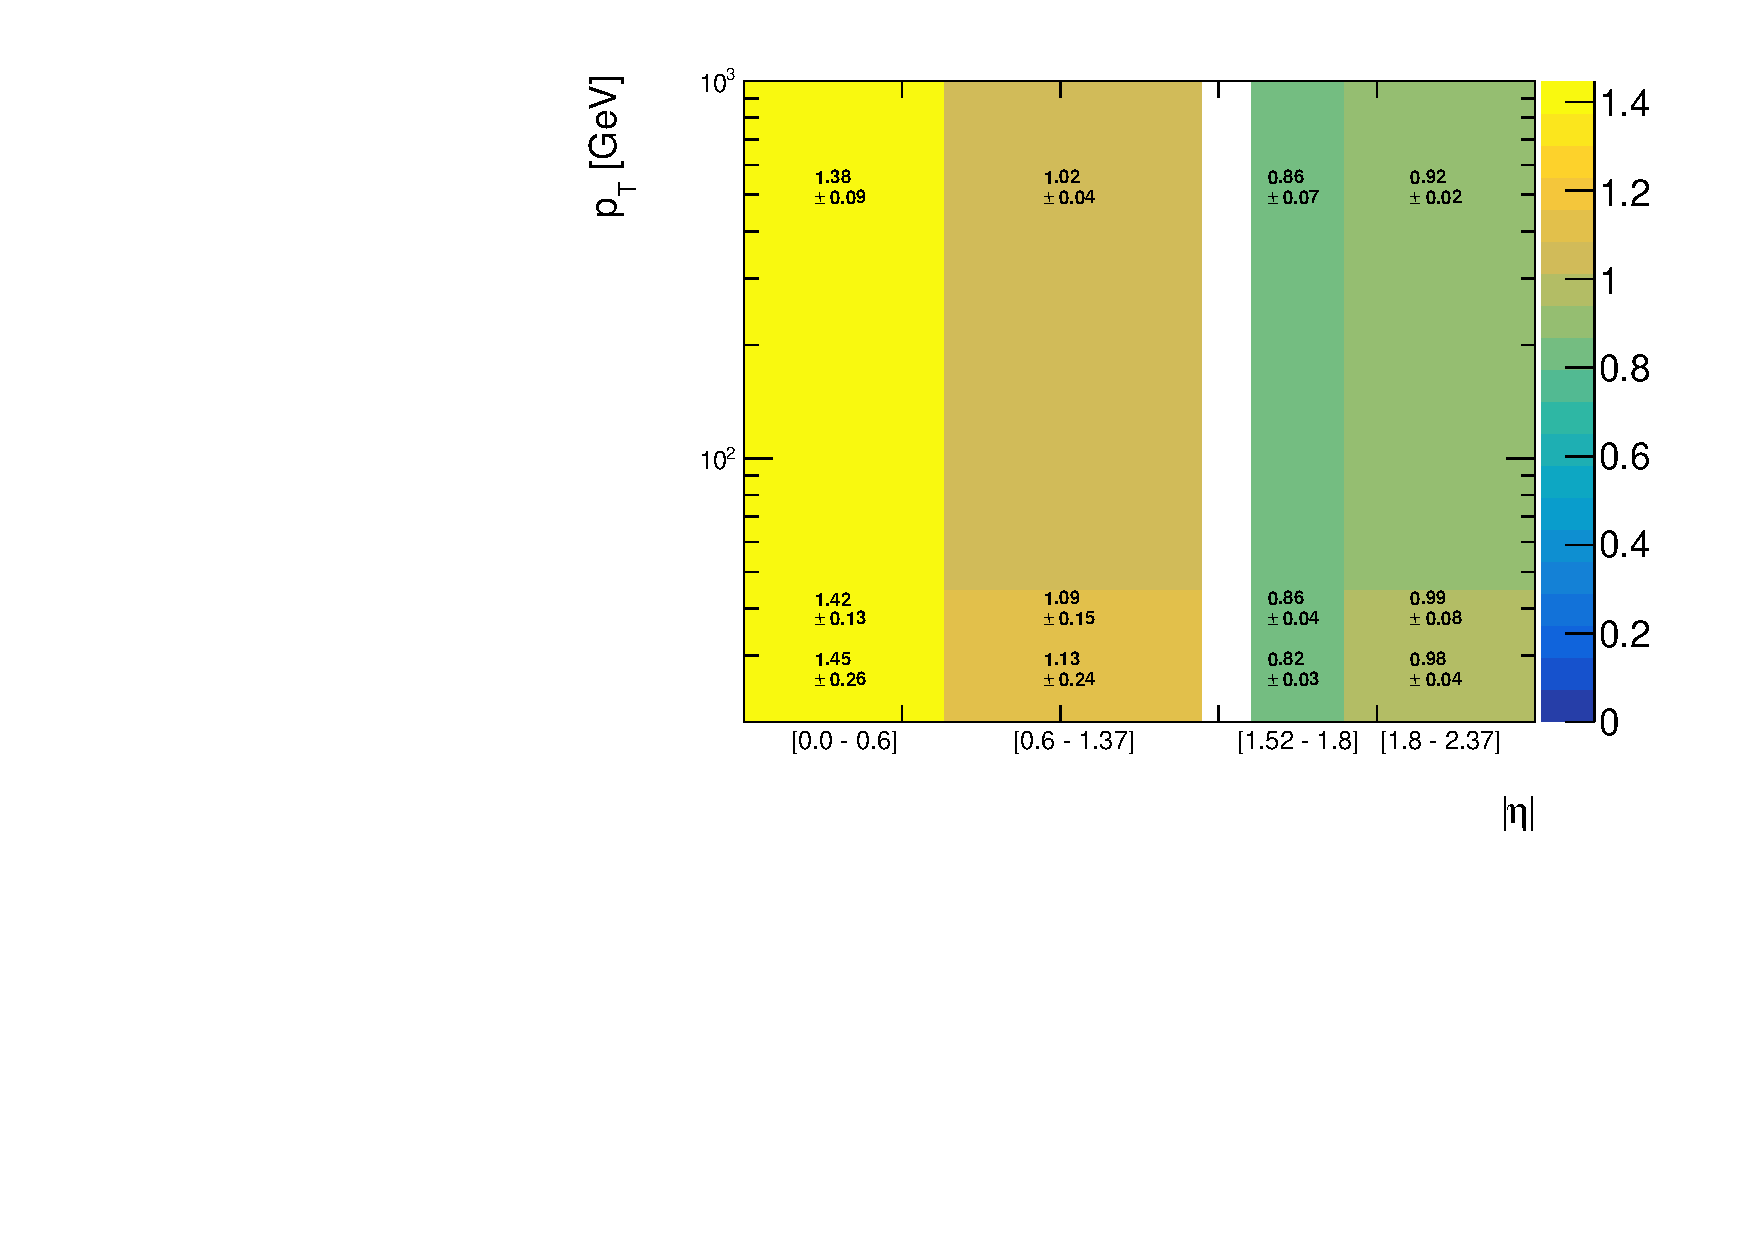
\includegraphics[width=0.7\textwidth]{figures/egammafakes/Map_EFake_SF_Final_converted.pdf}}
\caption [] {The final 2D fake rate scale factors with all uncertainties included (for converted photons).}
\label{fig:egammafake_ptetadiff_sfs_conv}
\end{figure}   
%---------------------------------------------- end efake SF for converted photon ---------------------------

%---------------------------------------------- efake SF for unconverted photon ---------------------------
\begin{figure}[!htbp]
\centering
{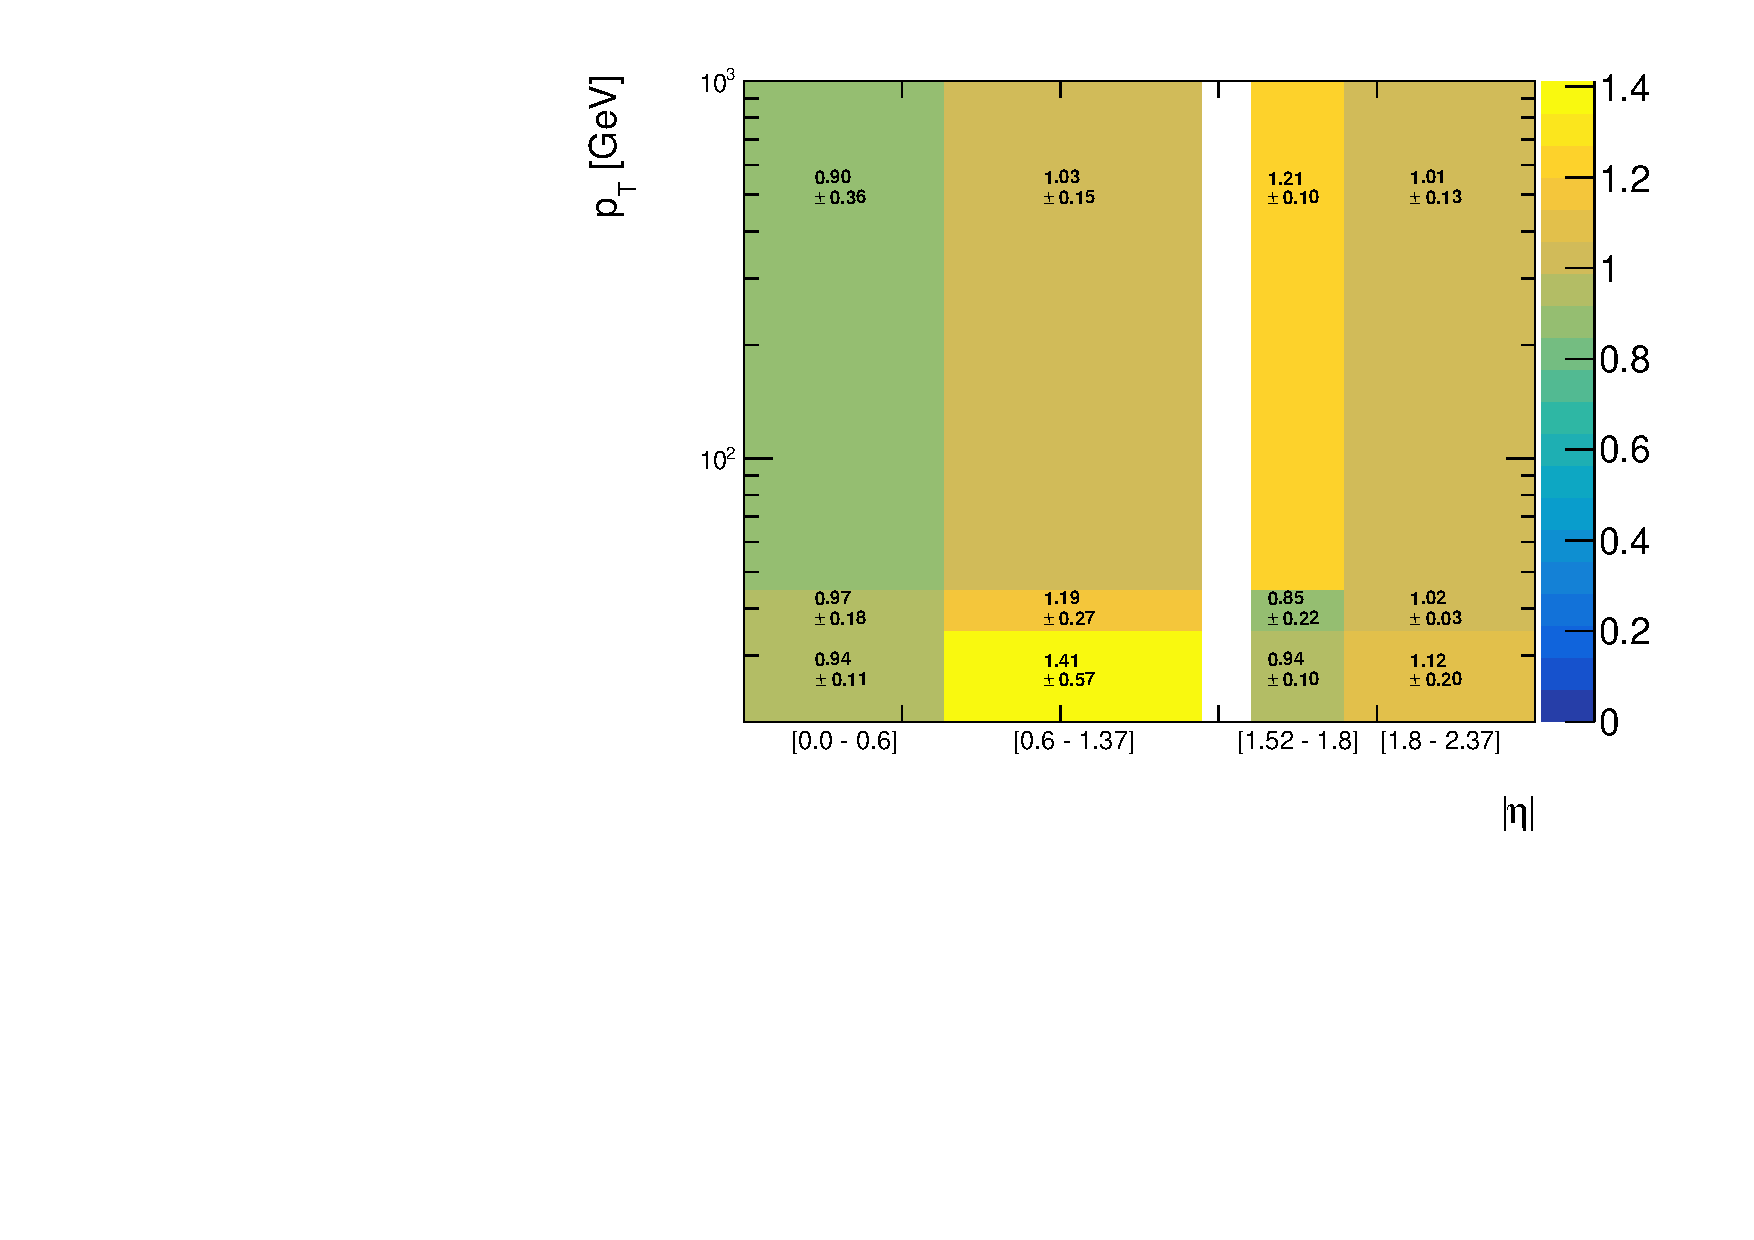
\includegraphics[width=0.7\textwidth]{figures/egammafakes/Map_EFake_SF_Final_unconverted.pdf}}
\caption [] {The final 2D fake rate scale factors with all uncertainties included (for unconverted photon).}
\label{fig:egammafake_ptetadiff_sfs_unconv}
\end{figure}   
%---------------------------------------------- end efake SF for unconverted photon ---------------------------

%--------------------------------------- impact of syst in SF -------------------------
\begin{figure}[!htbp]
\centering
\subfloat[]{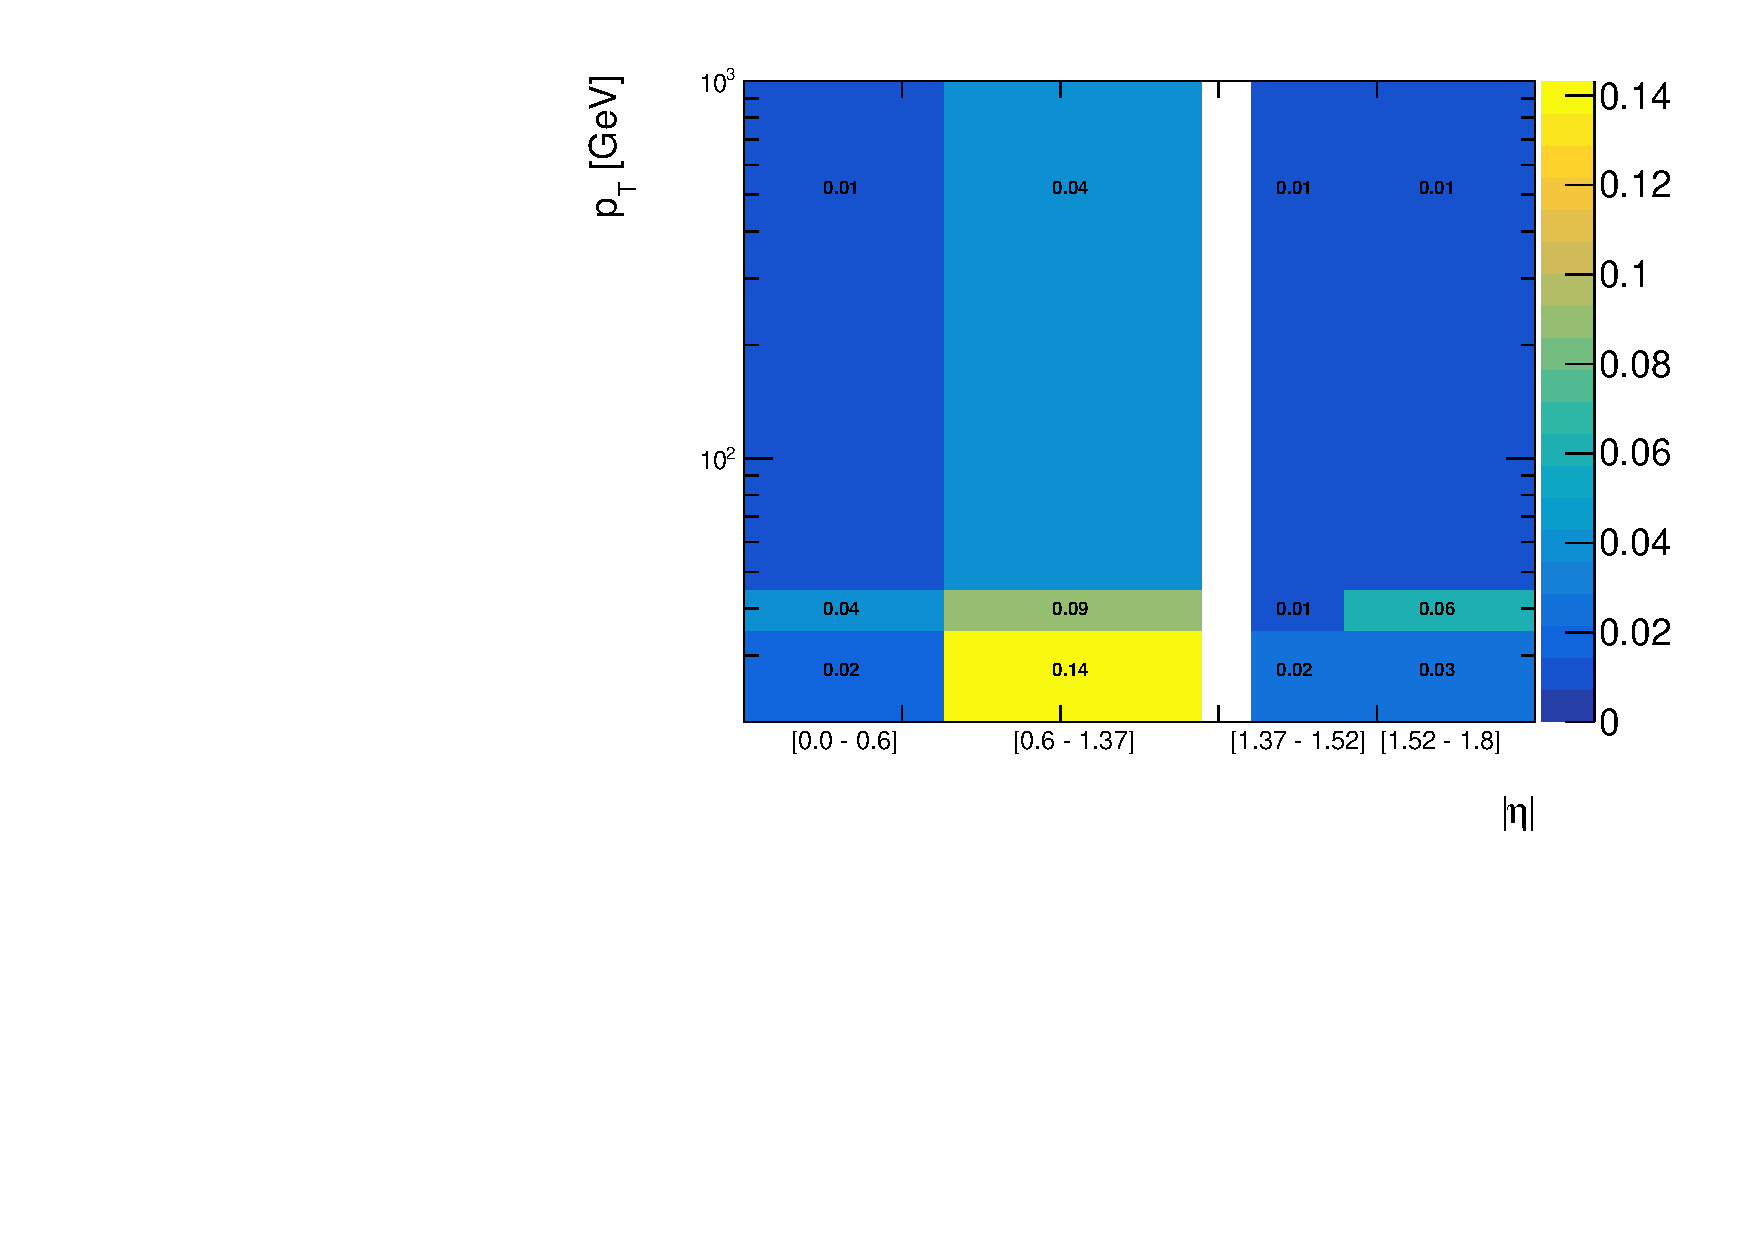
\includegraphics[width=0.45\textwidth]{figures/egammafakes/diffchangingSigtoMCtemplate.pdf}}
\subfloat[]{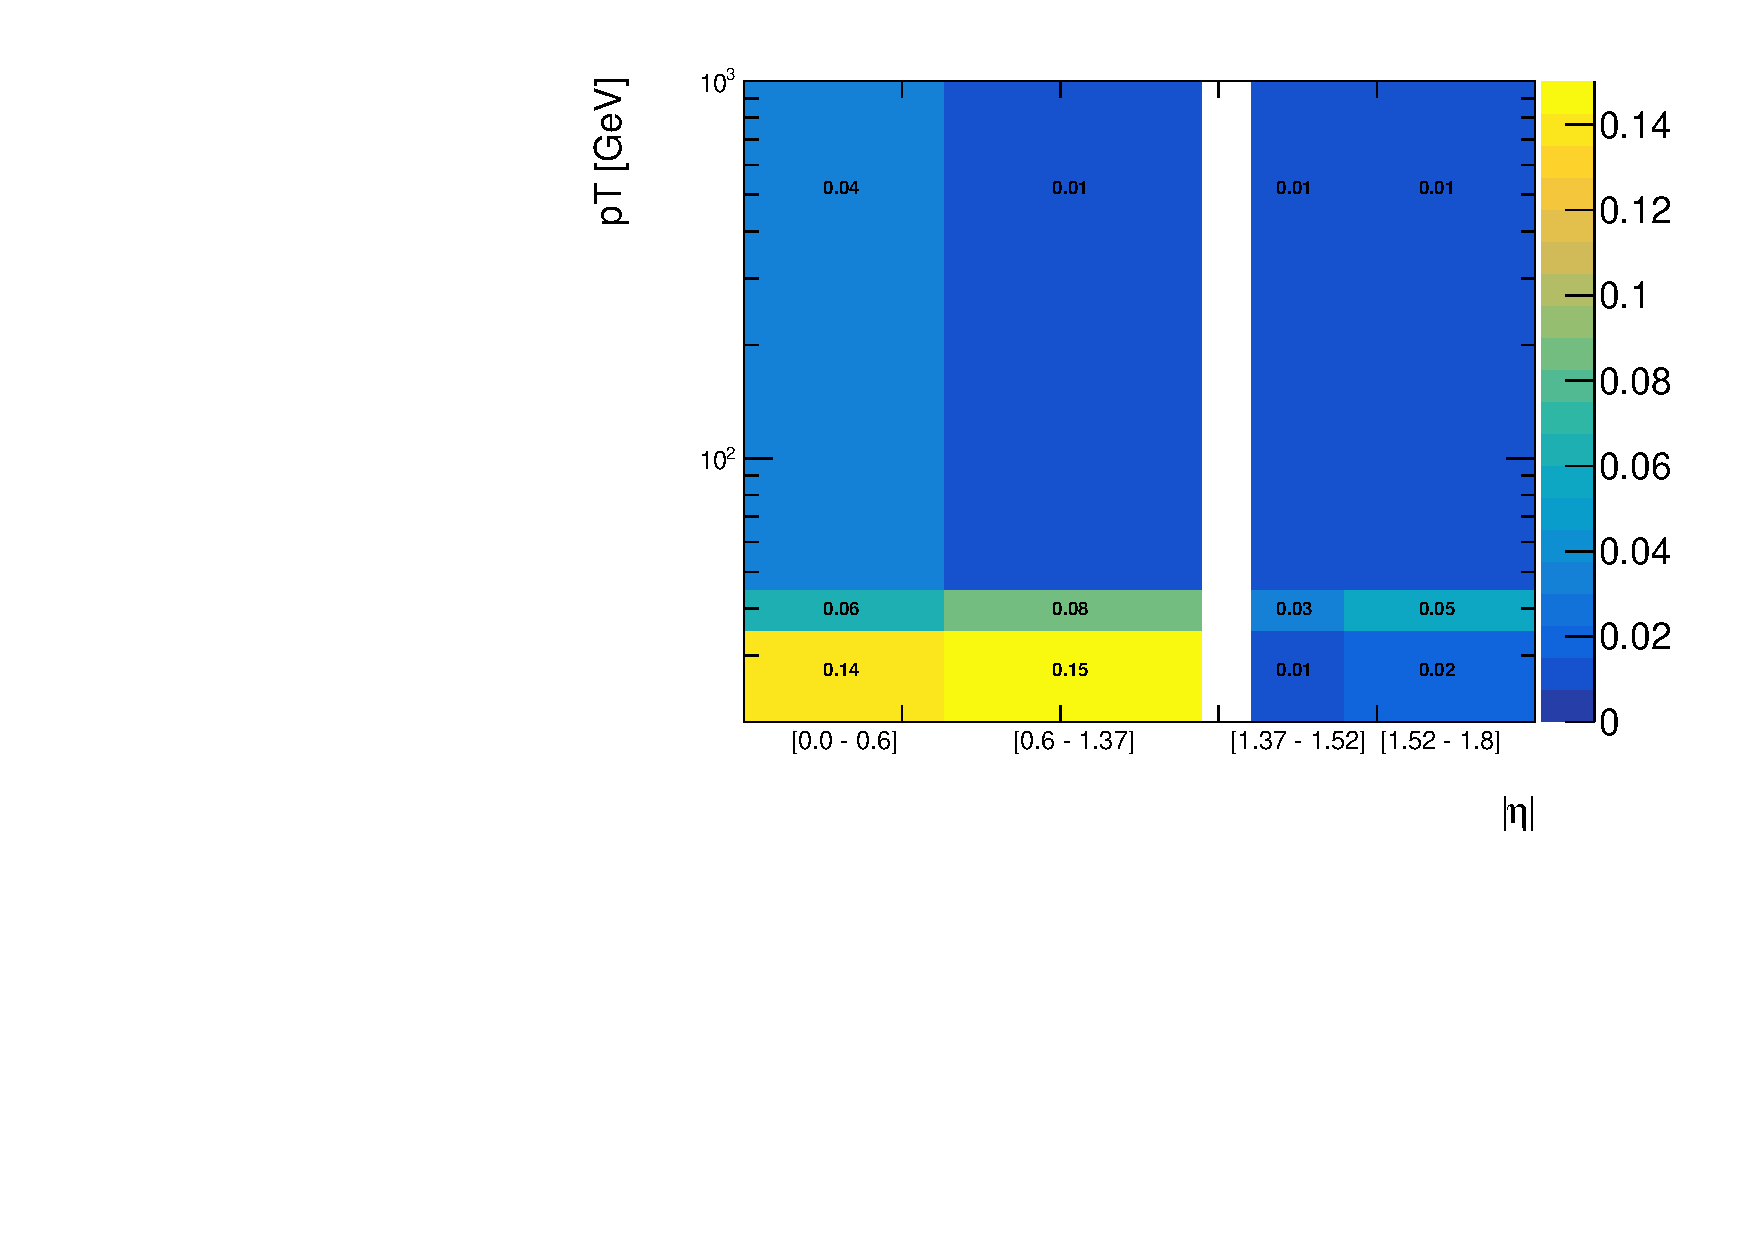
\includegraphics[width=0.45\textwidth]{figures/egammafakes/diffchangingBkgtoGaus.pdf}}
\quad
\subfloat[]{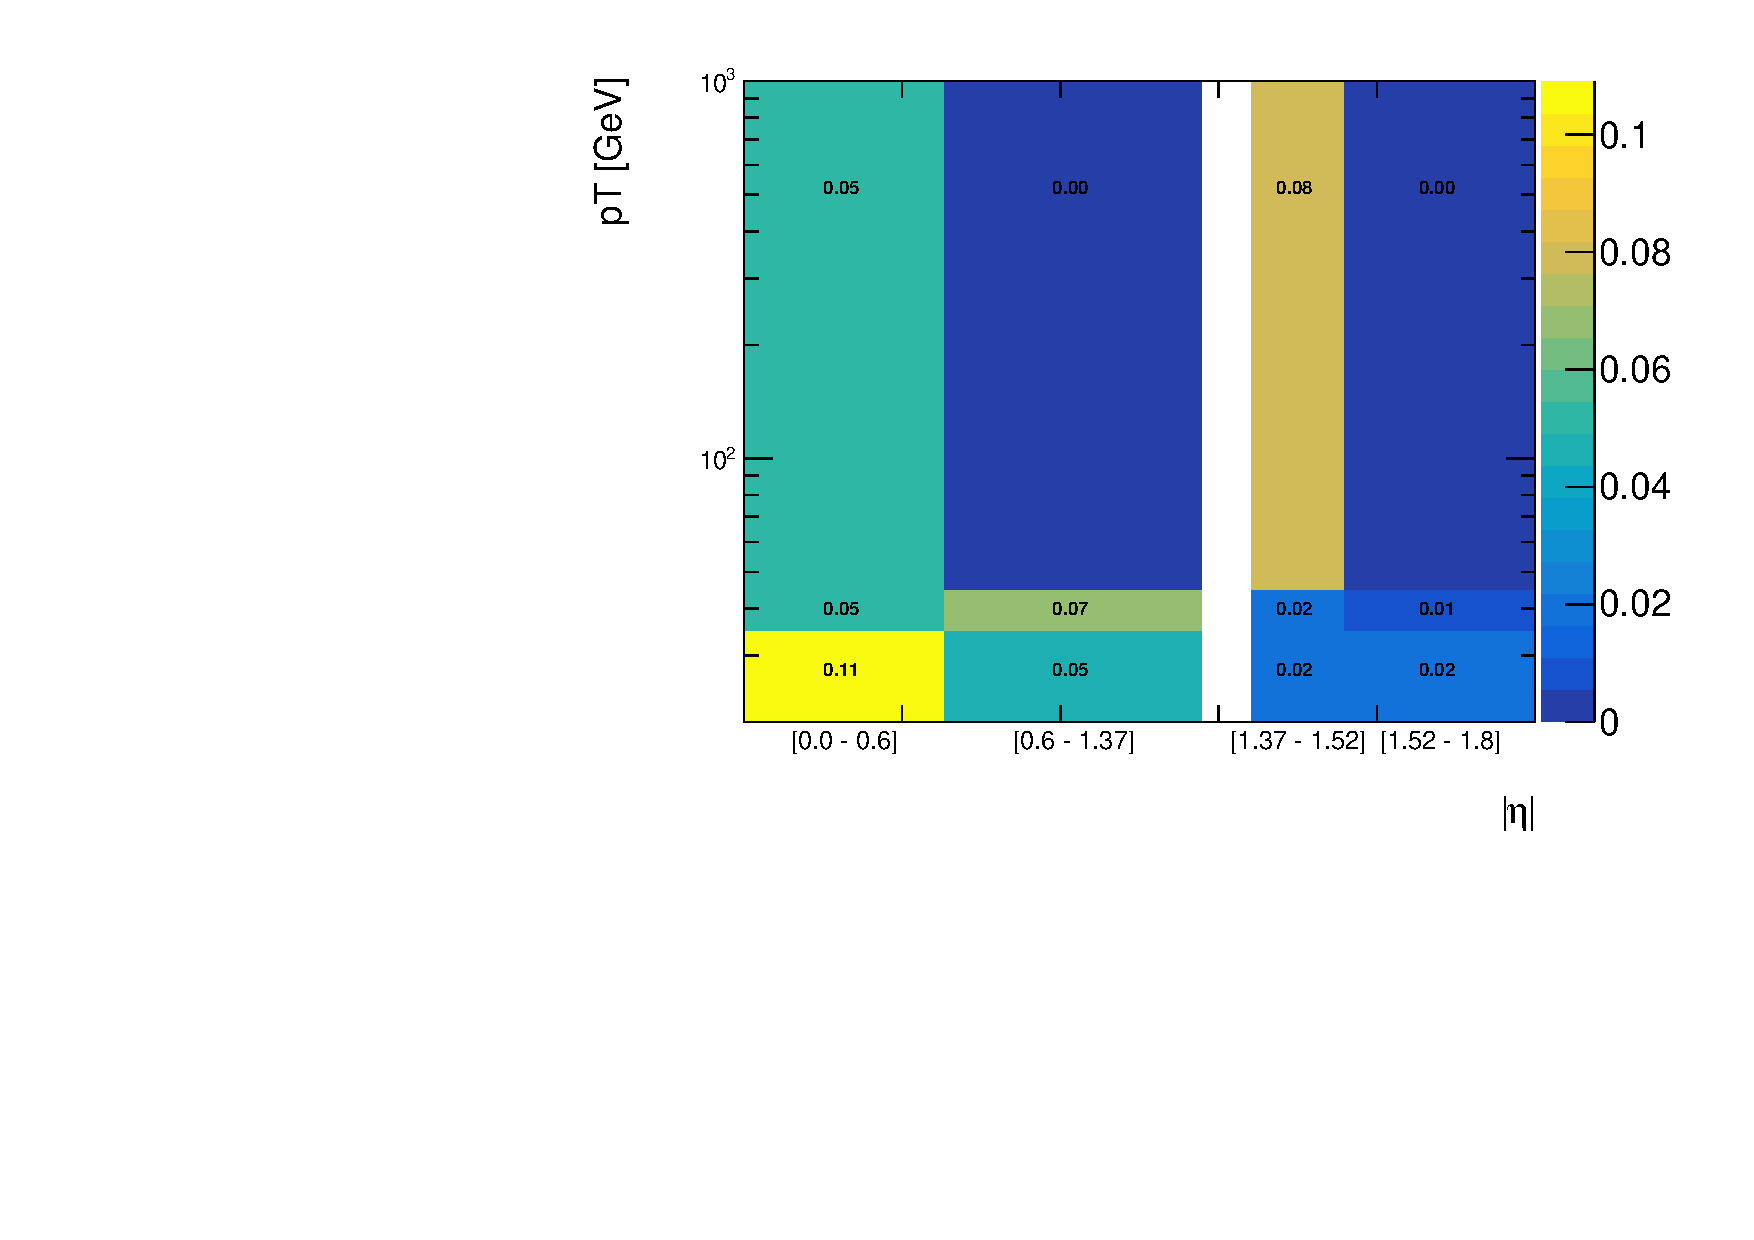
\includegraphics[width=0.45\textwidth]{figures/egammafakes/diffchangingMassWindow.pdf}}

\caption [] {Impact of the sources of systematic uncertainties for the converted photon case. The numbers show the relative uncertainty with respect to the nominal SFs in each bin. The sources of uncertainty are: (a) the signal function is changed to MC template. (b) the background function is varied to Gaussian. (c) variation of the fitting mass window in both sides by 5 GeV.}
%
%{\includegraphics[width=0.45\textwidth]{figures/egammafakesun/converted_ph/Postfit_Zpeak_PtBin1_EtaBin6_zee.pdf}}
%\phantomcaption 
\label{fig:impact_of_uncertainty_converted}
\end{figure}

\newpage

\begin{figure}[!htbp]
\centering
\subfloat[]{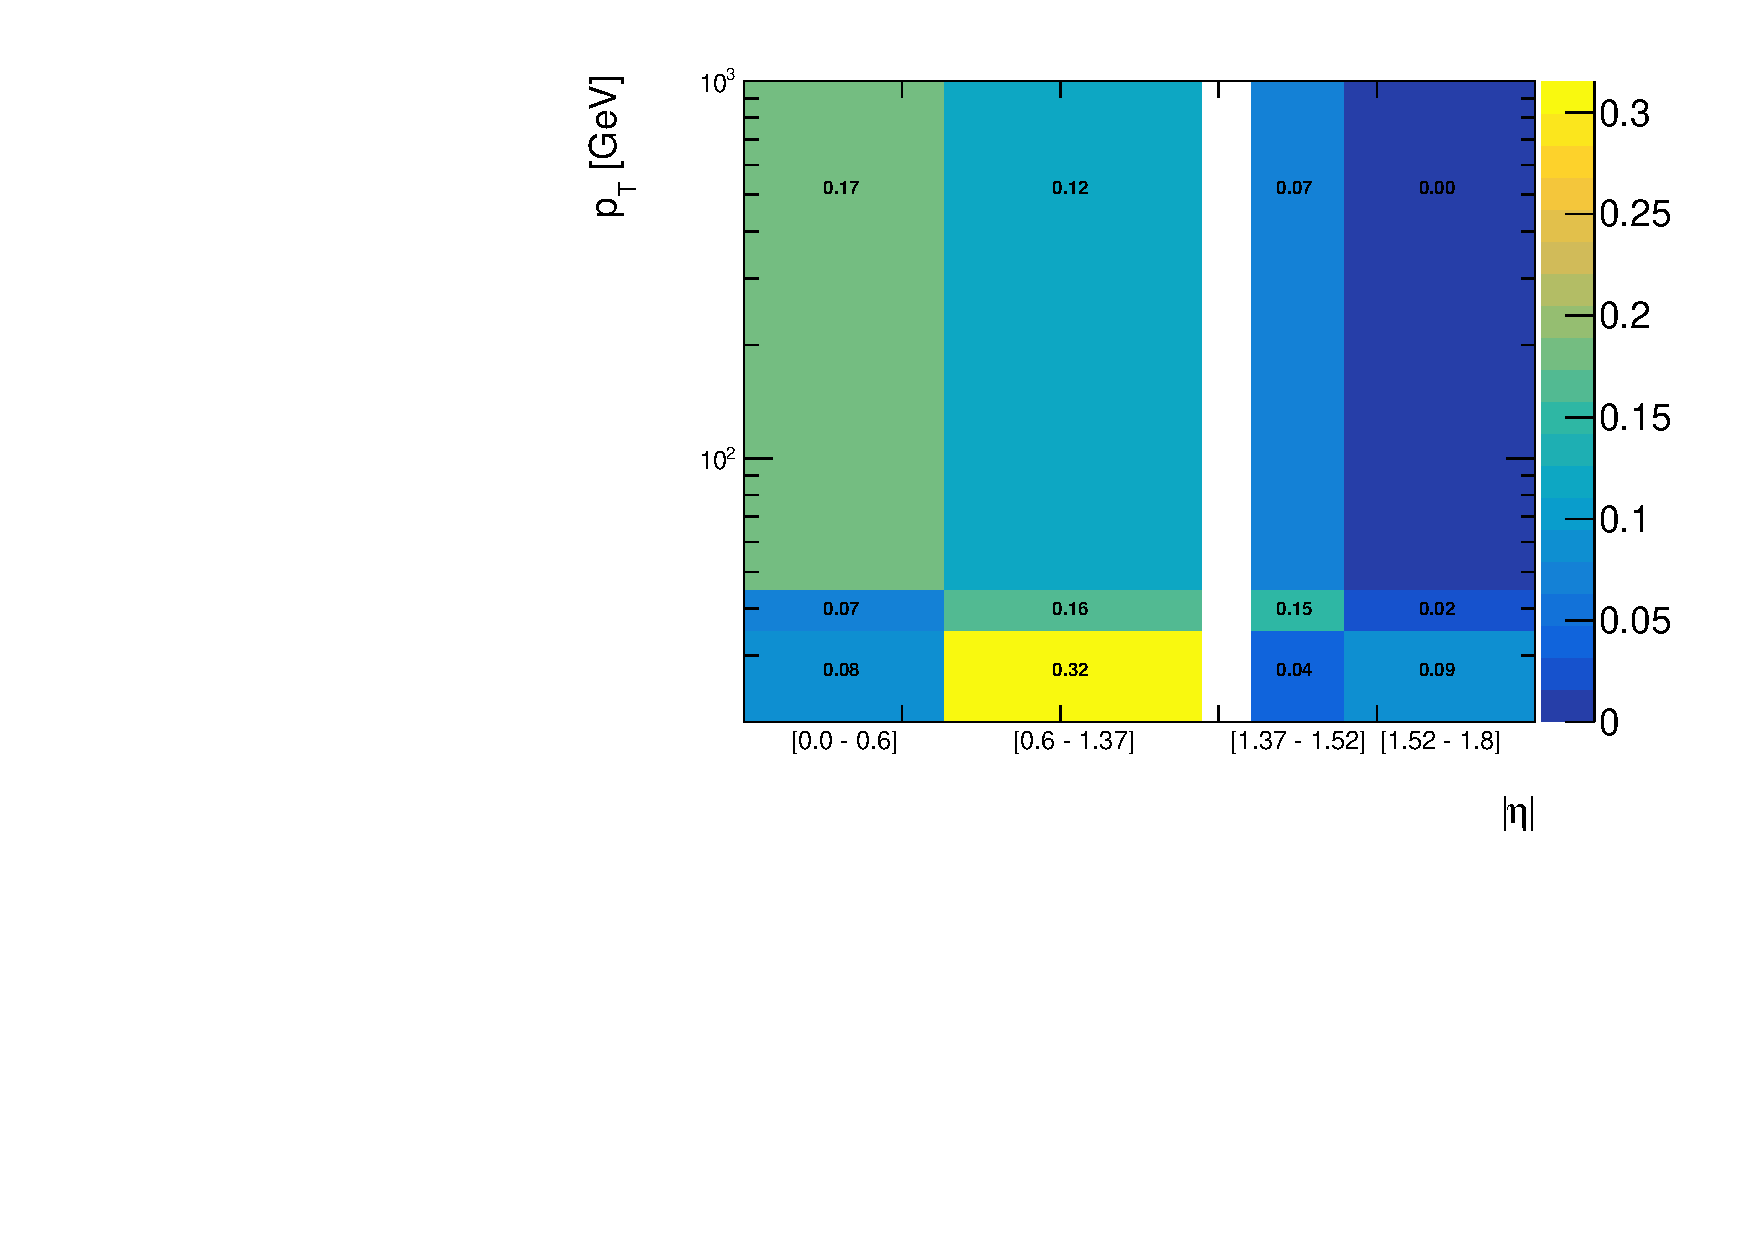
\includegraphics[width=0.45\textwidth]{figures/egammafakes/undiffchangingSigtoMCtemplate.pdf}}
\subfloat[]{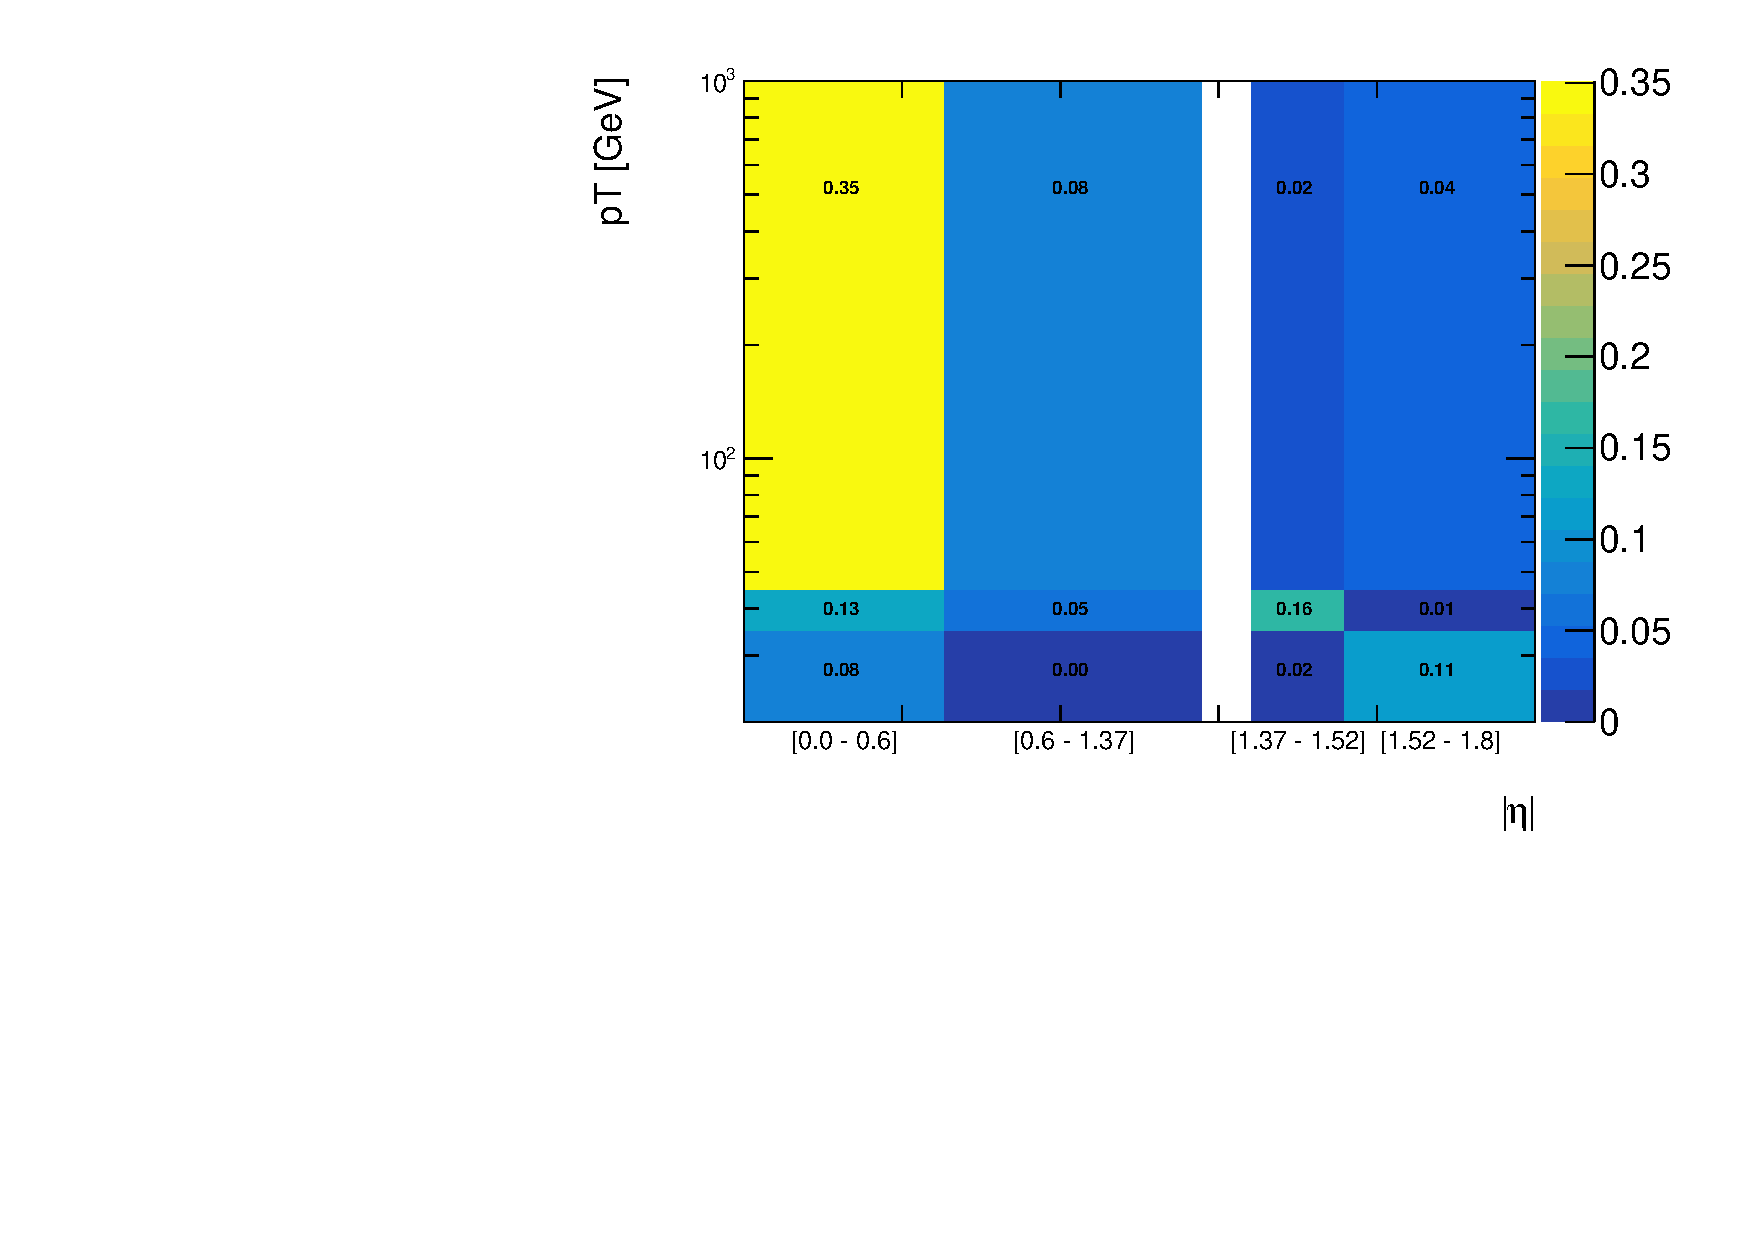
\includegraphics[width=0.45\textwidth]{figures/egammafakes/undiffchangingBkgtoGaus.pdf}}
\quad
\subfloat[]{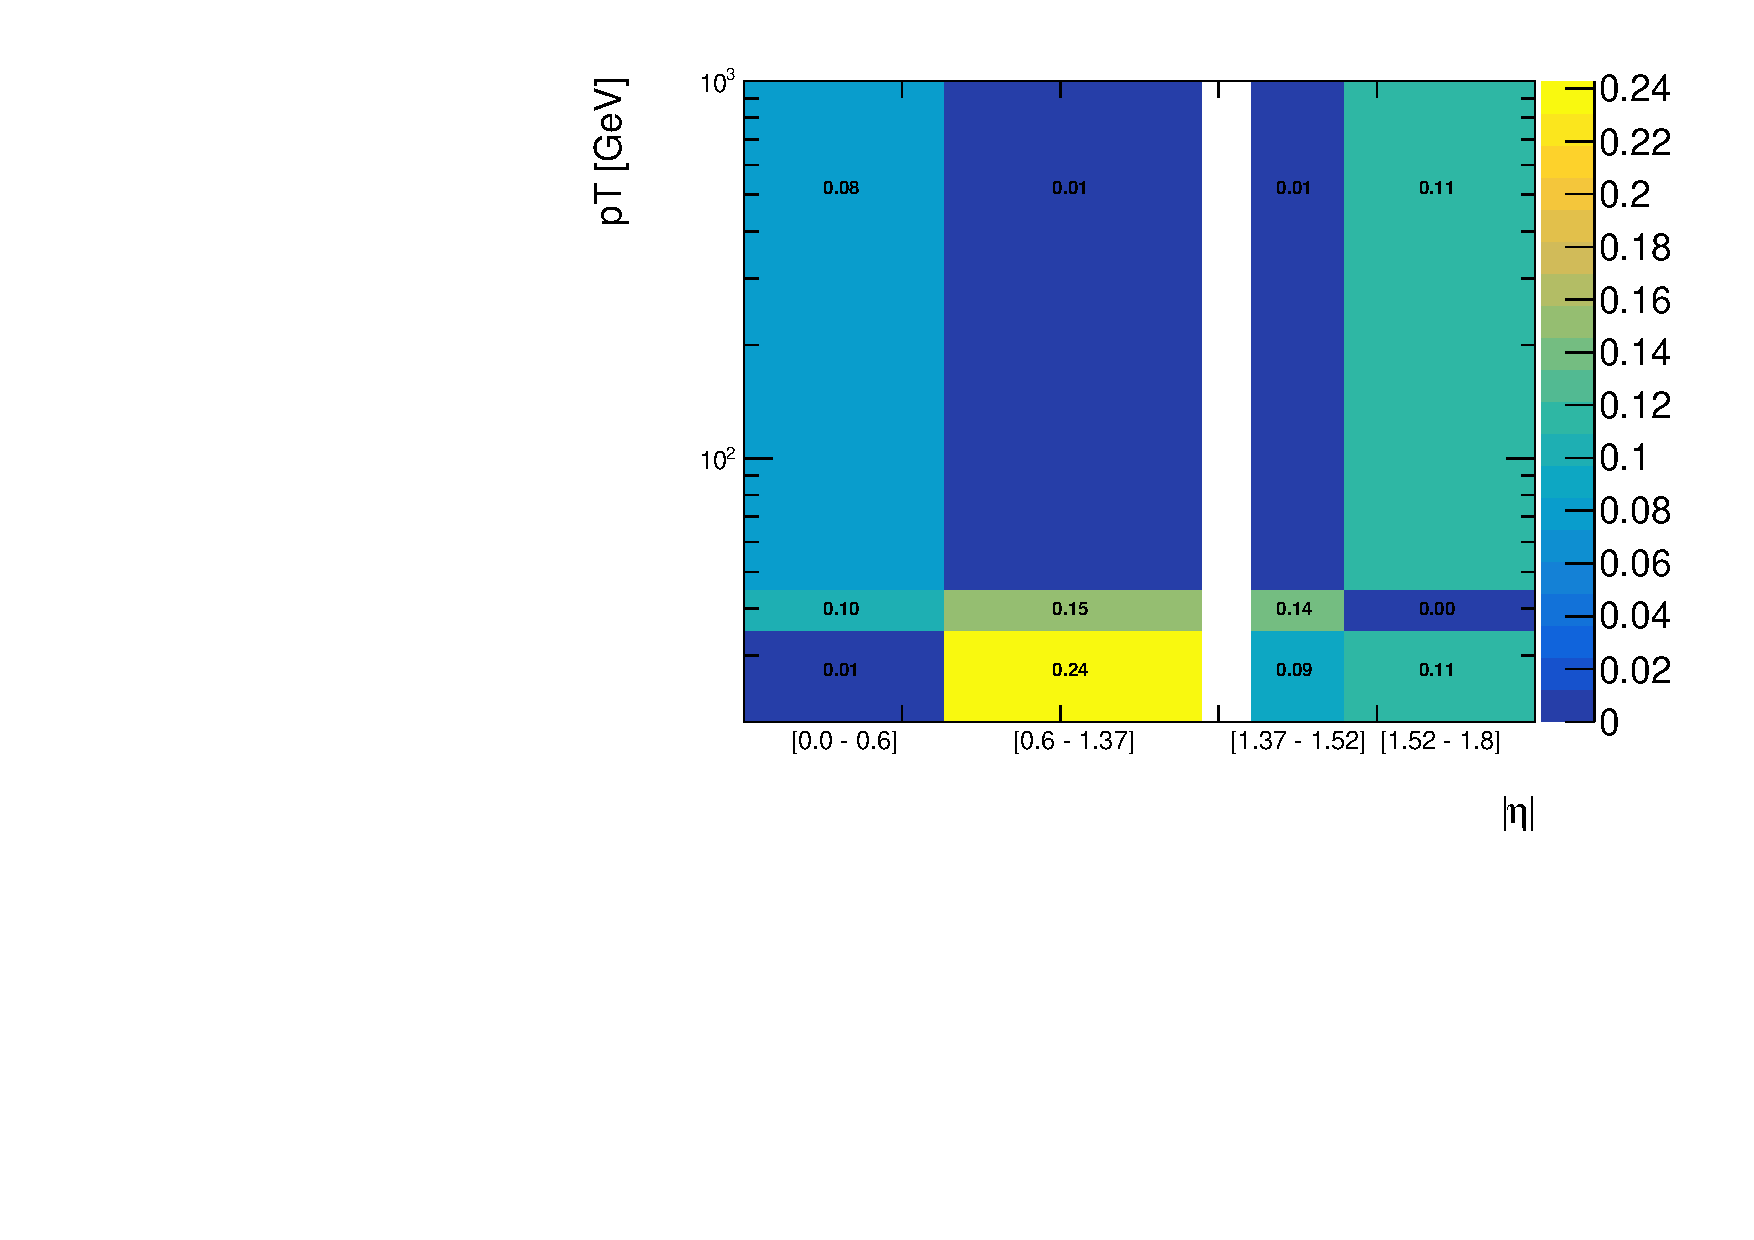
\includegraphics[width=0.45\textwidth]{figures/egammafakes/undiffchangingMassWindow.pdf}}

\caption[] {Impact of the sources of systematic uncertainties for the unconverted photon case. The numbers show the relative uncertainty with respect to the nominal SFs in each bin. The sources of uncertainty are: (a) the signal function is changed to MC template. (b) the background function is varied to Gaussian. (c) variation of the fitting mass window in both sides by 5 GeV.}
%{\includegraphics[width=0.45\textwidth]{figures/egammafakesun/converted_ph/Postfit_Zpeak_PtBin2_EtaBin6_zee.pdf}}
%\phantomcaption 
\label{fig:impact_of_uncertainty_unconverted}
\end{figure}

\FloatBarrier

\section{\hfake background estimation}
\label{sec:background-estimation-hfake}

Photon is reconstructed from the EM calorimeter clusters. The improper reconstruction and identification of photon can lead to misreconstruction of jet as photon. Also the photon coming from hadron decay can be misidentified and these events can enter our measurement. Together these events are referred as \hfake events. Mismodeling of these events is seen in MC when compared with the data. The scale factor is obtained by taking the ratio of the \hfake events in data and MC. The scale factor is then applied to the MC to correct for the mismodeling. 



\subsection{Fake lepton background estimation}
\label{sec:background-estimation-lfake}

 
\chapter{Sources of systematic uncertainties}
\label{sec:sources-of-uncertainties}
Uncertainties are an inherent part of any measurement, and it is important to properly account for them. There are several sources of uncertainties that need to be considered. These include statistical uncertainties, systematic uncertainties, and model uncertainties. Statistical uncertainties arise from the finite size of our data samples. In collider experiments, events occur randomly with a constant probability. The number of events in a given sample is a random variable that follows a Poisson distribution. The statistical uncertainty is the standard deviation of the Poisson distribution. This is inherent to the data and can only be reduced by increasing the size of the data sample meaning more integrated luminosity.

Systematic uncertainties, on the other hand, arise from imprecision in our experimental setup or analysis techniques. For example, the uncertainty can come from the particle reconstruction and identification, their energy and momentum measurement, luminosity measurement and so on.

Model uncertainties arise from the limitations of our theoretical models used to describe the data. MC event generation is used to generate event from a theoretical model. The uncertainty arises from the choice of the PDF set, the choice of the renormalization and factorization scales, the choice of the parton showering and hadronization models, and so on. Also, the cross-section of every process has an uncertainty associated with it. Different sources of uncertainties are discussed in the following sections. 

\paragraph{Treatment of uncertainties} As mentioned earlier the histogram templates obtained from MC simulated events are used for modelling the signal and background processes. MC templates are produced for different sources of uncertainties. The difference between the nominal template and systematic variation template taken as a measure of the uncertainty. % the question arises how we create the systematic variation templates?
In the statistical model (likelihood) different sources of uncertainties can be assumed as separate auxiliary measurements and can be incorporated in the likelihood function as nuisance parameters (NP), which are constrained to be within their uncertainties. For every source of uncertainty, one NP is added to the fit model. Uncertainties arising from different sources are treated as independent and uncorrelated. This means that the impact of one source of uncertainty does not affect the impact of another source. However, uncertainties within the same source are assumed to be correlated across different signal and control regions. Systematic uncertainties are modeled using Gaussian constraints. On the other hand, statistical uncertainties are modeled using Poisson constraints. The uncertainties associated with the nuisance parameters are estimated from the fit and propagated to the final results.
%discuss about morphing

\paragraph{Smoothing}The smoothing technique is used for some sources of uncertainties to reduce the impact of statistical fluctuations in the template.

\paragraph{Symmetrization}The are some uncertainties for which there are up and down variations w.r.t nominal is available and for some uncertainties only one variation is available. For asymmetric up and down variation, the variation is symmetrized to have a simpler implementation in the fit model. Uncertainties with up and down variations are symmetrized using the Two-Sided symmetrization method in the following way $$ \mathrm{symmetrized \ up/down} = \mathrm{nominal} \pm (\mathrm{up - down})/2 $$ In cases where only one variation is available, the other variation is obtained by mirroring the available one around the nominal. 

\paragraph{Pruning}Uncertainties with negligible impact are pruned from the fit model to avoid using too many NPs in the fit model. The pruning decision is made for shape and normalization components separately. The uncertainty can have a negligible impact on the normalization but a significant impact on the shape. In such cases, the uncertainty is pruned from the normalization component but kept in the shape component. It applies to the other way around as well. For pruning based on the normalization the integral of the template is considered and the relative difference between the nominal is calculated, if the relative difference is less than 0.1\% the uncertainty is pruned. For pruning based on the shape, the relative difference w.r.t nominal is calculated for every bin, if for any bin the difference is more than 0.1\% the uncertainty is kept.


\section{Experimental uncertainties}
\label{sec:experimental_uncertainties}
Experimental uncertainties arise from many sources these include uncertainties on the reconstruction and identification of physics objects, uncertainties on the energy and momentum scales and resolutions, uncertainties on the flavour tagging of jets, uncertainties on the integrated luminosity measurement, and uncertainties on the pile-up simulation. These affect both the signal and background simulations. 

\paragraph{Lepton efficiencies}
Electrons are reconstructed from the energy deposits in the calorimeter and the tracks in the inner detector. Muons are reconstructed combining the independent measurement in inner detector and muon spectrometer. Experimentally determined energy spectra are corrected with the selection efficiency, these include efficiency related to trigger, particle isolation, identification and reconstruction. The accuracy with which the detector simulation models the observed electron efficiencies is very important. Slight mismodelling is observed in the efficiencies between MC and in data. Using tag-and-probe approach and using \zee($\mu\mu$ for muons)  or \jpsiee($\mu\mu$ for muons) processes~\cite{ATLAS:2019jvq,ATLAS:2016lqx} the efficiencies are further corrected. Multiplicative scale factors are obtained from the ratio of efficiencies in data and MC. Scale factors are obtained in the bins of kinematic observables. The scale factors are applied to the MC to correct for the difference in efficiencies. The uncertainty on the estimated scale factors are used to create systematic variation templates.

\paragraph{Photon efficiencies}
Photons are reconstructed from the energy deposits in the calorimeter. The identification of prompt photon in the hadronic environment is challenging, because of the presence of overwhelming amount of  non-prompt photon from hadron decays. Prompt photons are identified with selection criteria on the shape and properties of the electromagnetic showers and also by requiring them to be isolated from other particles. These identification and isolation efficiencies in MC are further corrected using scale factors estimated using data-driven approach ~\cite{ATLAS:2016ecu,ATLAS:2019qmc}. The scale factors are varied up and down by their uncertainties to create systematic variation templates. 

\paragraph{$e,\mu,\gamma$ energy and momentum calibration}
Electrons and photon energy are measured from EM calorimeter clusters. The energy and momentum scale and resolution are calibrated using \zee decay and are validated using radiative $Z-$boson decays(details in~\cite{ATLAS:2019qmc}). The muon momentum is studied using \zmumu and \jpsimumu processes, and correction factors are derived to correct the muon momentum scale and resolution in MC to match with the data~\cite{ATLAS:2016lqx}. The uncertainties on the calibration are used to create systematic variation templates to propagate the uncertainties to the analysis.


\subsection*{Jet uncertainties}
% jets are reconstructed using the topo-cluster formed from the energy deposits in the calorimeter as well as from the tracks in the inner detector, combining these two information is referred to as ATLAS particle-flow algorithm.
% jets are first calibrated with sequence of simulation-based corrections then several in situ techniques are employed to correct the differences between data and simulation.
Jet reconstruction from the detector signature of the stable hadrons is described in~\cref{sec:physics_object_reconstruction}. The uncertainties comes mainly from the jet energy scale and resolution, jet vertex tagging. Jet energy scale which calibrates the jet energy with particle level energy of the jet. For this jets are calibrated first with sequence of simulation-based corrections then several \emph{in-situ} techniques are used to correct the differences between data and simulation. The individual steps correct various effects, such as, origin correction which corrects four momentum to point to primary vertex instead of pointing to the center of the detector, pile-up correction which removes the excess energy due to in-time and out-of-time pileup, absolute MC-based calibration which corrects jet 4-momentum to the particle-level energy scale, global sequential calibration which reduces flavor dependence and energy leakage effects using calorimeter, track and other variables. Finally a residual calibration is derived using \emph{in-situ} measurements and is applied only to data. The uncertainties may have many sources and are reduced to fewer effective nuisance parameter through eigenvector decomposition. Its uncertainty is split into several independent categories: modelling and statistical uncertainties on the extrapolation of the jet calibration from the central region, jet flavour composition, high-\pT jet behaviour, \bjet energy scale uncertainties, uncertainties due to pile-up, uncertainties on \textit{in situ} jet energy corrections, etc. In one category, there are usually more than one physical source of the uncertainty. To study the JES uncertainty, each source is varied up and down independently by its corresponding uncertainty. 

The jet energy resolution (JER) is measured using the balance between jets and well measured objects like photons or $Z$ bosons, and it is found to be in agreement between data and MC. There are a total of seven effective nuisance parameters associated to JER in the category reduction scheme, and a single source of uncertainty for the agreement between data and Monte Carlo, all of which are varied by one sigma to study their impact on the analysis.

The systematic uncertainty associated to the jet vertex tagging (JVT) is obtained by varying up and down the JVT cut using the \emph{JetVertexTaggerTool}~\cite{ATLAS-CONF-2014-018}. 


\subsection*{\btag uncertainties}

Jets coming from a \bquarks have their own topological features, and \btag allows to distinguish them from light-flavour jets. With \emph{\btag}, each jet can be assigned to a different working point, and the \btag uncertainties on this jet are derived for this specific working point. They are accounted for by varying the calibration scale factors for \ensuremath{b}-,\ensuremath{c}-, and light-flavour jets up and down by their corresponding systematic uncertainties independently. For each jet category, the uncertainties are decomposed into several uncorrelated components using the eigenvector method. As pseudo-continuous \btag weights are used the corresponding eigenvectors are used, which results in 45 nuisance parameters for \bjets and 20 nuisance parameters for \cjets and light-flavour jets each~\cite{ATL-PHYS-PUB-2017-013}.
%For example, there are 9, 4 and 4 eigenvectors for \bjets, \cjets and light-flavour jets uncertainties, respectively~\cite{ATL-PHYS-PUB-2017-013}.
As the pseudo-continuous b-tagging is only calibrated for b-jets below 400 GeV, c-jets below 250 GeV and light jets below 300 GeV, a normalisation uncertainty was assigned to events containing at least one uncalibrated jet. For each type of jets one uncertainty was defined and for each event containing an uncalibrated jets of that type (b-jet, c-jets or light jet) a 50\% uncertainty was assigned. This leads to three systematic uncertainties.

\subsection*{Missing transverse momentum}

The \met is reconstructed~\cite{ATLAS-CONF-2018-023} from the vector sum of several terms corresponding to different types of reconstructed objects. The estimated uncertainties for electrons, muons, photons and jets are propagated into the uncertainty of \met. Thus, the only new contribution is the systematic uncertainty of the soft terms $E_{\text{x,y}}^{\text{RefSoftJet}}$ and $E_{\text{x,y}}^{\text{CellOut}}$.

The systematic uncertainty of the soft-term scale is estimated by comparing the ratio of Monte-Carlo simulation to data. The average deviation of the ratio from unity is taken as a flat uncertainty on the absolute scale. The systematic uncertainty of the soft-term resolution is estimated by evaluating the level of agreement between data and MC in the $E^{\text{miss}}_{\text{x}}$ and $E^{\text{miss}}_{\text{y}}$ resolution. Both the scale and resolution of the soft term are varied up and down by one standard deviation to study their impact on the analysis. 

\subsection*{Pile-up uncertainties}

The uncertainty on the reweighting procedure used to correct the pile-up profile in MC to match the data, is based on the disagreement between the instantaneous luminosity in data~\cite{DAPR-2013-01} and in simulation. Both the nominal and systematically-shifted pileup-reweighting weights are obtained using the standard \texttt{PileupReweighting} tool~\footnote{More details: \url{https://twiki.cern.ch/twiki/bin/viewauth/AtlasProtected/ExtendedPileupReweighting}.}. 

\subsection*{Luminosity uncertainties}

As quoted in \cref{sec:selection}, the total integrated luminosity has an uncertainty of \intlumiunc.



\subsection{Model uncertainties}
\label{sec:theoretical_uncertainties}




\chapter{Measurement of the \tty cross-sections} % Main chapter title
\label{Chapter8} % Change X to a consecutive number; for referencing this chapter elsewhere, use \ref{ChapterX}

\section{Fiducial phase space}
\label{sec:fiducial-phase-space}
The measurements are performed at particle level in a fiducial phase space volume. Particle level refers to final state particles after the parton showering and hadronization but prior to any interaction with the detector apparatus. The fiducial regions in the single lepton and dilepton final states are defined to closely follow the kinematic requirements at reconstruction level. The objects are defined as follows:
\begin{itemize}
\item Photons: Photons are required to not originate from a hadron decay, to have $p_T > \SI{20}{\GeV}$ and $|\eta| < \SI{2.37}{}$ and to be isolated such that the sum of transverse momenta of all charged particles surrounding the photon within $\Delta R \leq$ 0.2 must be smaller than 5\% of its own \pt.
\item Leptons: Electrons and muons are dressed with close by photons (photons which are not originating
from hadrons, in a $\Delta R <0.1$ cone around the lepton). Leptons are required to have \pt $>$ 25 GeV
and $|\eta|<$ 2.5, and not being originated from hadron decays.
\item Jets: Jets are clustered with the anti-kt algorithm with a radius of R = 0.4. Non-interacting particles and
muons are not considered in the clustering. Jets are required to have \pt $>$ 25 GeV
and $|\eta|<$ 2.5
\item b-jets: A particle-level jet is identified as a $b$-jet if a hadron with $\pT > \SI{5}{\GeV}$ containing a $b$-quark is matched to the jet through a ghost-matching method~\cite{Cacciari:2008gn}.
\item The overlap removal among the different objects is performed in the following order:
\begin{itemize}
\item Muon-jet: Jets with $\Delta R(\mu, j)\leq 0.4$ are removed.
\item Electron-jet: Jets with $\Delta R(e, j)\leq 0.4$ are removed.
\item Photon-jet: Jets within $\Delta R( j, \gamma) \leq 0.4$ of an isolated photon are removed.
\end{itemize}
\end{itemize}

The fiducial phase space in the single-lepton channel is defined by requiring exactly one photon, exactly one electron or muon, at least four jets among which at least one is a $b$-jet. In the case of the dilepton channels, it is defined by requiring exactly one photon, exactly two leptons (electron or muon), at least two jets among which at least one is a $b$-jet.



\section{Differential cross-section measurement}
\label{sec:diff-xsec-measurement}
The cross-section is measured within a defined fiducial phase space volume (\cref{sec:fiducial-phase-space}) at particle level as a function of different observables listed in \cref{tab:listvariables}. The cross-section at the particle level is derived using an unfolding technique. Unfolding is used to extract the truth spectrum from the reconstruction level spectrum correcting the detector effects such as limited resolutions, efficiency and acceptance effects, making the results easier to compare with the theoretical predictions. We implement the profile likelihood unfolding method for this purpose, detailed in \cref{sec:profile-likelihodd-unfolding}. 

Ideally, a continuous functional dependence of the measurement would be preferable. However, the finite detector resolution prevents this. Consequently, we measure the cross-section in discrete bins. For more information on how the bins are chosen detailed in \cref{sec:choice-of-binning}.

\begin{table}[ht]
\caption{The differential cross sections are measured in single-lepton channel and dilepton channel as a function of the following variables: }
\label{tab:listvariables}
\begin{footnotesize}
\begin{tabular} {r l }
  Symbol & Defintion \\
  \hline
  Both dilepton and single lepton channels: & \\
  \hline 
  \pt($\gamma$) & Transverse momentum of photon \\ 
  $|\eta|$($\gamma$) & Absolute value of the pseudorapidity of the photon \\
  \DRlph & Angular separation between the photon and the closest lepton \\
  $\Delta R_{min}(\gamma, b)$ &  Angular separation between the photon and the closest $b$ jet \\
  $\Delta R_{min}(l, j)$ & Smallest angular separation between any of the selected leptons and jets \\
  $p_T(j_1)$ & Transverse momentum of the leading jet\\

  \hline
  Additional variables for dilepton channel: & \\
  \hline
  $\Delta R(\gamma, l_1)$ & Angular separation between the photon and the leading lepton\\
  $\Delta R(\gamma, l_2)$ & Angular separation between the photon and the subleading lepton\\
  \Detall & Pseudorapidity difference between the two leptons\\
  \Dphill & Azimuthal angle difference between the two leptons\\
  $p_T(l,l)$ & Transverse momentum of the dilepton system\\
  $p_T(j_1)$ & Transverse momentum of the leading jet\\
    
\end{tabular}

\end{footnotesize}
\end{table}
\FloatBarrier

As detailed in profile-likelihood unfolding section[\ref{sec:profile-likelihodd-unfolding}], the histogram templates at the reconstruction level are used as the inputs for the unfolding, where the signal histograms are obtained by folding the truth distributions with the response matrix. To take into account the uncertainties response matrices are constructed for every source of systematic uncertainties for signal and varied histogram templates (at the reconstruction level) are produced for background templates. More details on how the truth distributions and response matrices are constructed are detailed in \cref{sec:inputs-for-unfolding}.

Before the unfolding procedure is applied to the real data various tests are performed beforehand using the pseudo-data. This approach validates the unfolding procedure and avoids any post-unfolding modifications to the model, which could introduce bias. Here pseudo-data refers to the sum of all MC templates including signal and backgrounds. Two tests are performed, closure test and stress test. In the closure test, the pseudo-data is unfolded and compared with the truth distribution of the signal, and a good closure is observed (more on closure test in \cref{sec:closure_test}). This validates that the unfolding procedure using response matrix and truth distribution can correctly measure the signal from the dataset (in this case pseudo-dataset). The signal normalization and shape shape in real data can be different than in MC simulation. Unfolding using MC truth distribution and response matrix (which is derived from MC simulation) can introduce bias while measuring the signal from the real data. The stress test mentioned in \cref{sec:stress_test} validates that the unfolding procedure is very robust and can measure the signal correctly from the data even if the shape of the signal present in the data is different than in MC simulation. 

After validating the unfolding procedure, fit and unfolding is performed on the real data to measure the cross-section. The results are detailed in \cref{sec:tty_prod_measurement}, \cref{sec:tty_total_measurement} and \cref{sec:tty_prod_sldl_measurement} for \tty production measurement, inclusive \tty measurement and \tty production measurement in a combined single lepton and dilepton channel respectively.

\subsection{Profile likelihood unfolding}
\label{sec:profile-likelihodd-unfolding}
\paragraph{Unfolding procedure}
The reconstruction level spectrum $y$ can be written in terms of the truth spectrum $x$ as $$ y = R x$$, where $R$ is the response matrix. The standard unfolding procedure involves the inversion of the response matrix to obtain the truth spectrum. It becomes difficult when the matrix is not easily invertible. Instead, we follow a different approach in which standard profile likelihood fitting is used for unfolding ~\cite{cls_3}. The TRExFitter framework \emph{TRExFitter}\footnote{\url{https://trexfitter-docs.web.cern.ch/trexfitter-docs/}} is used for the fitting and unfolding process. In this approach, the truth distribution comprising N bins is multiplied by the corresponding response matrix (\ref{sec:inputs-for-unfolding}) of size N x M, thereby transforming the truth distribution into a reconstruction level distribution with M bins. A normalization factor is assigned for each bin of the truth distribution, these factors are parameters of interest (POI). It is important to note that the normalization of these folded distributions on the reconstruction level is identical to the normalization of the truth distribution. Therefore, by measuring the normalization factors for each bin of each folded distribution on the reconstruction level, the normalization of the truth level is directly obtained, thus we obtain the cross-section at the truth level. Standard profile likelihood fit is performed to obtain the POIs. A toy example to illustrate the unfolding procedure is shown in Figure~\ref{fig:unfolding_toy_example}.

%generate code to add a figure
\begin{figure}[ht]
    \centering
    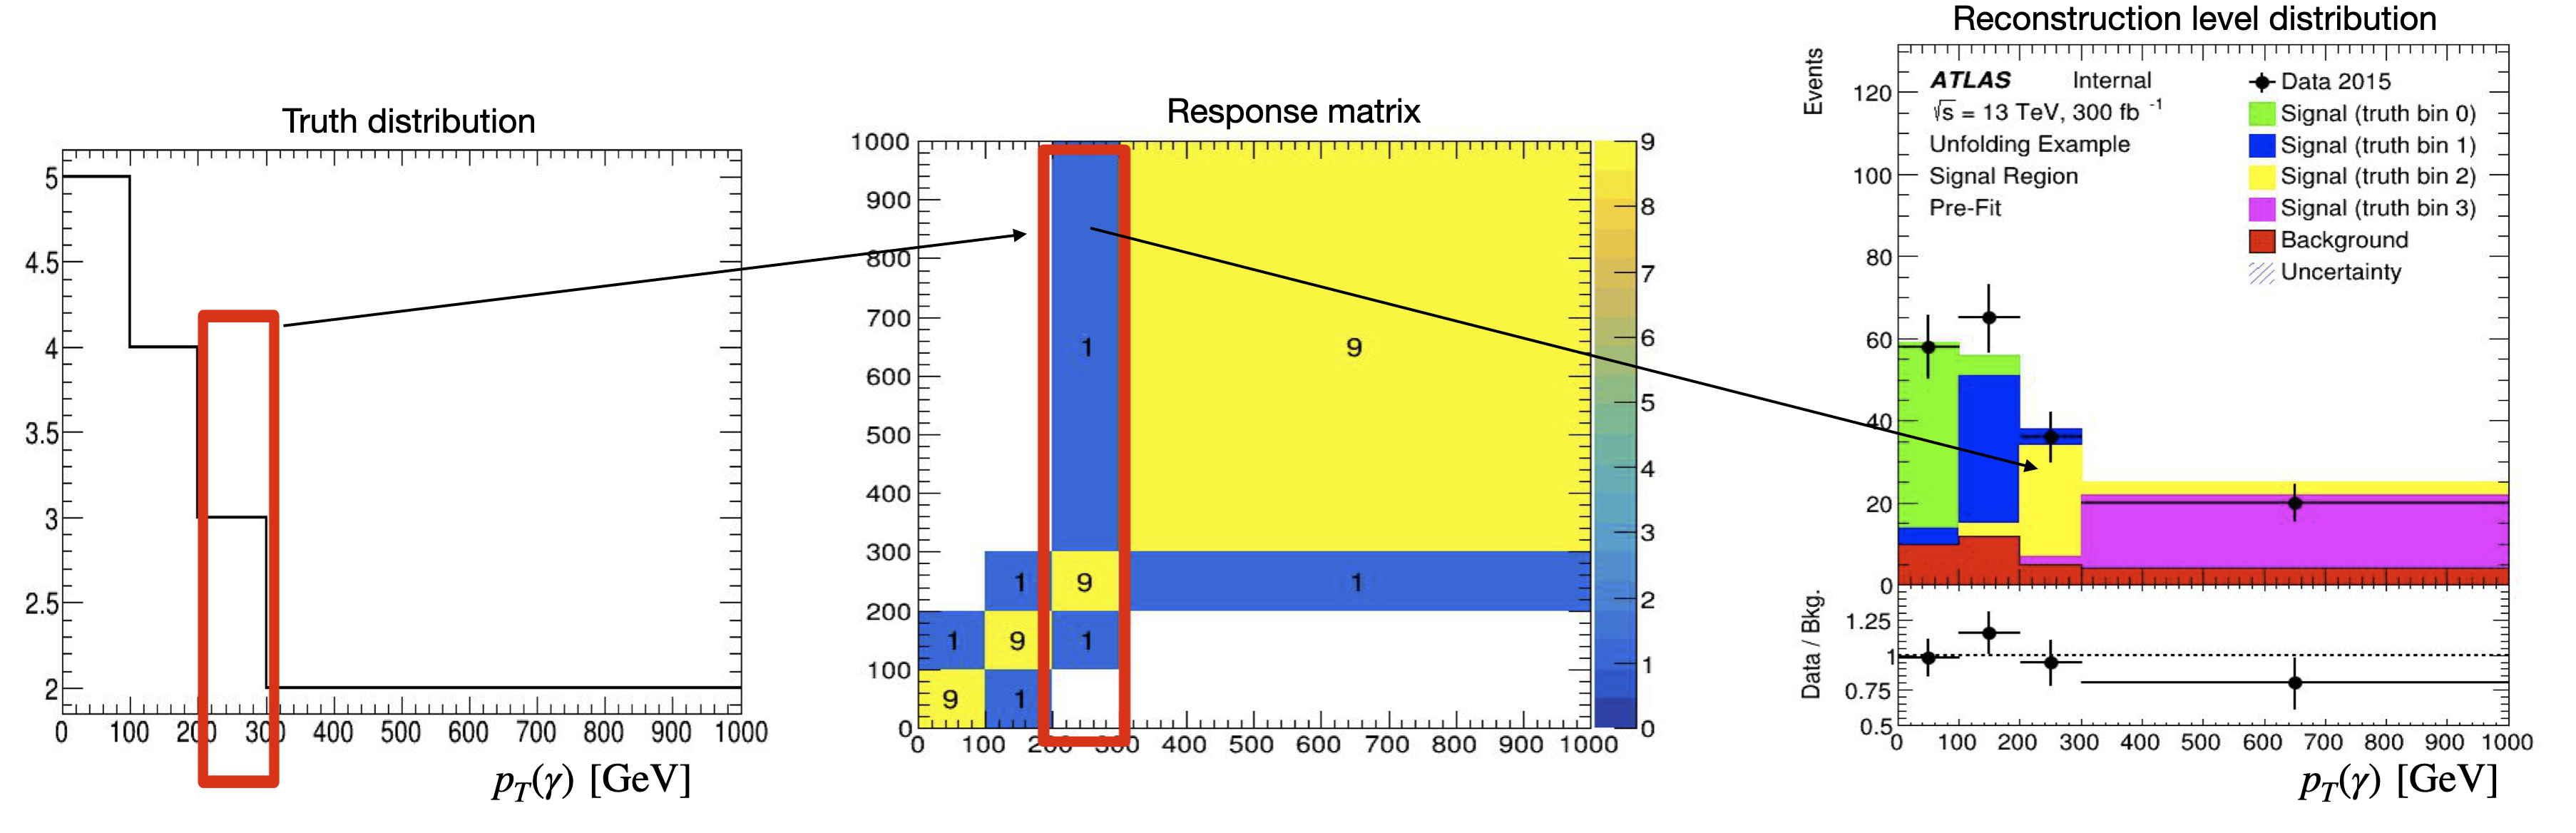
\includegraphics[width=0.9\textwidth]{figures/toy_profile_likelihood_fit.png}
    \caption{Toy example to illustrate the unfolding procedure. The truth distribution is multiplied by the response matrix to obtain the distribution at the reconstruction level. A normalization factor is assigned for each bin of the truth distribution. Profile likelihood fit is performed to the reconstruction level distribution to obtain the normalization factors. The truth distribution is directly obtained from the normalization factors.}

    \label{fig:unfolding_toy_example}
\end{figure}
\FloatBarrier

\paragraph{Likelihood construction}
In \emph{TRExFitter} the likelihood is constructed using the \textsc{histfactory}~\cite{Cranmer:2012sba} which is used to build parametrized probability density functions in the RooFit/RooStats framework [todo cite] using simple ROOT histograms. The likelihood is constructed using the truth histogram and the response matrix for signal and histogram templates at the reconstruction level for backgrounds, as below:
\begin{equation}\label{eq:likelihodd-defn}
	L(\vec{n}^{data} | \vec{k}, \vec{\theta}) = \prod_{\mathrm{c} \epsilon \mathrm{Region}} \quad \prod_{\mathrm{b} \epsilon \mathrm{Bins}} \mathrm{Pois} (n^{\mathrm{data}}_{b,c}|\nu_{b,c}(\vec{k}, \Vec{\theta})) \cdot \prod_{p} \mathrm{Gauss}(0|\theta_{p},1)
\end{equation}

where,\\ 
- \textit{Region} refers to the different signal and control regions,\\
- \textit{Bins} refers to the bin of the reconstruction level histogram,\\
- $n^{\mathrm{data}}_{b,c}$ is the data in bin \textit{b} and region \textit{c}, \\
- $\nu_{b,c}$ is the expected total events in bin \textit{b} and channel \textit{c}, \\
- $\Vec{\theta}$ are the constrained nuisance parameter describing systematic uncertainties [\ref{sec:sources-of-uncertainties}] and $\mathrm{Gauss}(0|\theta_p,1)$ is a Gaussian constraint for the NP $\theta_p \in \vec{\theta}$ with mean of 0 and standard deviation of 1,\\
- $\vec{\mu}$ are the unconstrained parameters (e.g. POIs).

$\nu_{b,c}$ can be expressed as follows:

\begin{align}\label{eq:likelihodd-defn-1}
    \nu_{b,c} = \left[\sum_i \gamma_{b,c,i} \cdot \mu_{i} \cdot R_{b,c,i} \cdot T_{i}\right] + \sum_{B} \gamma_{b,c}^{B} \times N_{b,c}^{B} 
\end{align}

where, \\
- $\gamma$ factors are the bin-by-bin scale factors for MC statistical uncertainties. The background samples each have the factors $\gamma_{b,c}^{B}$, and for the signal each truth bin has a unique $\gamma_{b,c,t}$\\
- $R_{b,c,t}$ are the response matrices of the signal, calculated from the particle level and reconstruction level events \\
- $\mu_{i}$ corresponds to the signal strength of the bin $T_{i}$ at particle level.

% mention the later story, the minimization and so on.
% how errors are calculated

\paragraph{Likelihood minimization} The next step in the fitting procedure is the minimization of the negative log-likelihood. This is performed using \textsc{minuit} framework[todo cite] which uses \textsc{migrad} and \textsc{minos} minimization technique. The minimization process adjusts the POIs and NPs to find the set of values that best fit the observed data. The fit yields the uncertainties on the estimated POIs, correlations among POIs and between POIs and NPs.

%The uncertainties on the POIs are determined by profiling the likelihood. In this approach, the likelihood is profiled over all NPs. The uncertainty on each POI is obtained by finding the parameter values that change the log-likelihood by 0.5 from the minimum value. This corresponds to a 1$\sigma$ uncertainty on the POI. In this method, both statistical and systematic uncertainties are taken into account. 
%The statistical uncertainties are obtained using similar approach but keeping the NPs fixed to their nominal value.


\subsection{Choice of binning}
\label{sec:choice-of-binning}
The choice of the binning depends on several factors, the bin width of each bin must be greater than the resolution of the observable in that range and the statistical uncertainties in every bin of the measured distribution are small enough to avoid large fluctuations. To achieve this, two criteria were chosen to determine the bin widths. The bin width is chosen such that it is larger than twice the resolution of the observable and that the expected statistical uncertainty in the measured distribution is below 10\%. The algorithm starts with a finer binned histogram at the reconstruction level and starts to merge the bin from left to right till the statistical uncertainty reaches below 5-7\% (depending on the observable). This process is performed only considering the signal region (at the reconstruction level) due to the complexity of the profile likelihood unfolding across multiple reconstruction regions. After determining the binning edges through the algorithm, the fit and unfolding are performed and finally the statistical uncertainty is verified at the unfolded distribution. A crucial consideration is that the binning choice should exceed twice the resolution of the variable, as stated above. The resolution for the variable $\pt(\gamma)$, $|\eta(\gamma)|$, $\Delta R(\gamma,l)$, $\Delta R(\gamma,b)$, $\Delta R_{min}(l,j)$, $\Delta \eta(l,l)$, $\Delta \phi(l,l)$, $\pt(j_1)$, $\pt(l,l)$ are found to be around 1-2 GeV, 0.1-0.15, 0.005-0.008, 0.014-0.020, 0.01, 0.0006, 0.0003, 10 GeV, 2-3 GeV, respectively. The optimized bin widths based on the statistical uncertainty fullfilled in all cases the resolution criterion. During binning optimization, we observed slight statistical fluctuations in some bins, which can be attributed to the complexities of fit and unfolding across regions. For those cases the bin boundaries were slightly adjusted as well as to have simpler bin edges (e.g. multiples of 0.1, 5, 10 depending on the distribution). 

This study is performed for \tty(prod) and \tty(total) measurements in dilepton channel. The results are compared among the two sets and with the binning used by CMS measurement ~\cite{CMS2022}. The bin boundaries showed significant similarities. Testing our unfolding setup against CMS binning revealed that the unfolded distributions met the set criteria, yielding in general similar uncertainties and migrations. Consequently, we adopted the CMS binning, allowing a more conducive comparison in the future. For illustration, the resolution and comparison of two setups for some example variables can be found in appendix~\ref{sec:binning_optimization_study}. The same binning was applied to the l+jets channel. 

The unfolded $\pt(\gamma)$ distribution is used as input for the EFT measurement combining the single lepton and dilepton fiducial phase spaces as mentioned in section {ToDo: add ref}. The binning for this variable was revised to improve the sensitivity in the EFT measurement, increasing the number of bins while keeping the total expected uncertainty in the tail of the distribution around 10\%, which is most sensitive to the EFT parameters.  



\subsection{Inputs for unfolding}
\label{sec:inputs-for-unfolding}
As inputs to the unfolding, binned distribution of the observable at particle level as well as the response matrix are needed. Binned distributions at the particle level are obtained after applying the particle level event selection outlined in \cref{sec:event-selection}. These distributions are depicted in \cref{fig:folding_input_ljet} for the single lepton channel and in \cref{fig:folding_input_dilep1} for the dilepton channel. The bin content, represented by $T_{i}$, serves as input for the Likelihood function described in \cref{eq:likelihodd-defn-1}.

\paragraph{Response matrix} The response matrix effectively translates particle level distribution to the reconstruction level distribution taking into account factors like selection efficiency, detector acceptance and migration of events to neighboring bins. Essentially, when the response matrix is applied to the truth distribution it yields distribution at the reconstruction level. Response matrix is constructed from particle level to each region in reconstruction level, resulting in 4 response matrices for single lepton channel and 2 for dilepton channel. Furthermore, response matrices are obtained for each source of uncertainty. These matrices are formulated using the migration matrix ($N_{r \cap t}$), which relates the reconstructed and truth level distributions for the respective variable, along with the corresponding truth ($N_{t}$) and reconstructed ($N_{r}$) distributions in the following way:
\begin{align}
    \text{Response, } P_{r,t} = \frac{M_{\mathrm{r,t}} \times \epsilon_{t}}{f_{r}}\\
    = \frac{\frac{N_{r \cap t}}{\sum_{r} N_{r \cap t}} \times \frac{\sum_{r} N_{r \cap t}}{N_{t}}}{\frac{\sum_{t} N_{r \cap t}}{N_{r}}}\\
    = N_{r \cap t} \times \frac{N_{r}}{N_{t}\times \sum_{t} N_{r \cap t}}
\end{align}

where, \\
$M_{\mathrm{r,t}}$ is the normalised Migration matrix (as shown in \cref{fig:folding_input_migration_dilep}, \cref{fig:folding_input_migration_ljet}),\\
$\epsilon_{t}$ is the efficiency of the truth events and \\
$f_{r}$ is the acceptance of the reconstructed events

\vspace*{20pt}

For illustration, the normalized migration matrices for $p_T(\gamma)$ in the different signal and control regions are shown in \cref{fig:folding_input_migration_ljet} and \cref{fig:folding_input_migration_dilep} for the single lepton and dilepton channels, respectively. The response matrices for $p_T(\gamma)$  are shown in \cref{fig:folding_input_response_ljet_pt1} and \cref{fig:folding_input_response_dilep} for single channel and dilepton channel respectively. Additionally in \cref{fig:folding_input_response_ljet_pt1} and \cref{fig:folding_input_response_dilep} data-MC Comparison plots are shown where the signal is reconstructed by folding the truth distribution with the response matrix. 

The signal histogram is obtained at the reconstruction level using truth distribution and response matrix. The histogram templates for backgrounds are also used as inputs for the fit and unfolding. The background templates are constructed using the MC samples described in [todo ref] and applying the signal and control region selection criteria and merged into categories as described in the \cref{sec:photon-categorisation}. The background templates enter in the likelihood function following the equation \cref{eq:likelihodd-defn-1}.
%The migration matrices, response matrices and data-MC comparison plots for other observables are shown in Section ~\ref{sec:results_others_ljet} for the single lepton channel and in Section ~\ref{sec:results_others_dilep} for the dilepton channel.




\begin{figure}[ht]
    \centering
    % ph pt
    \subfloat[]{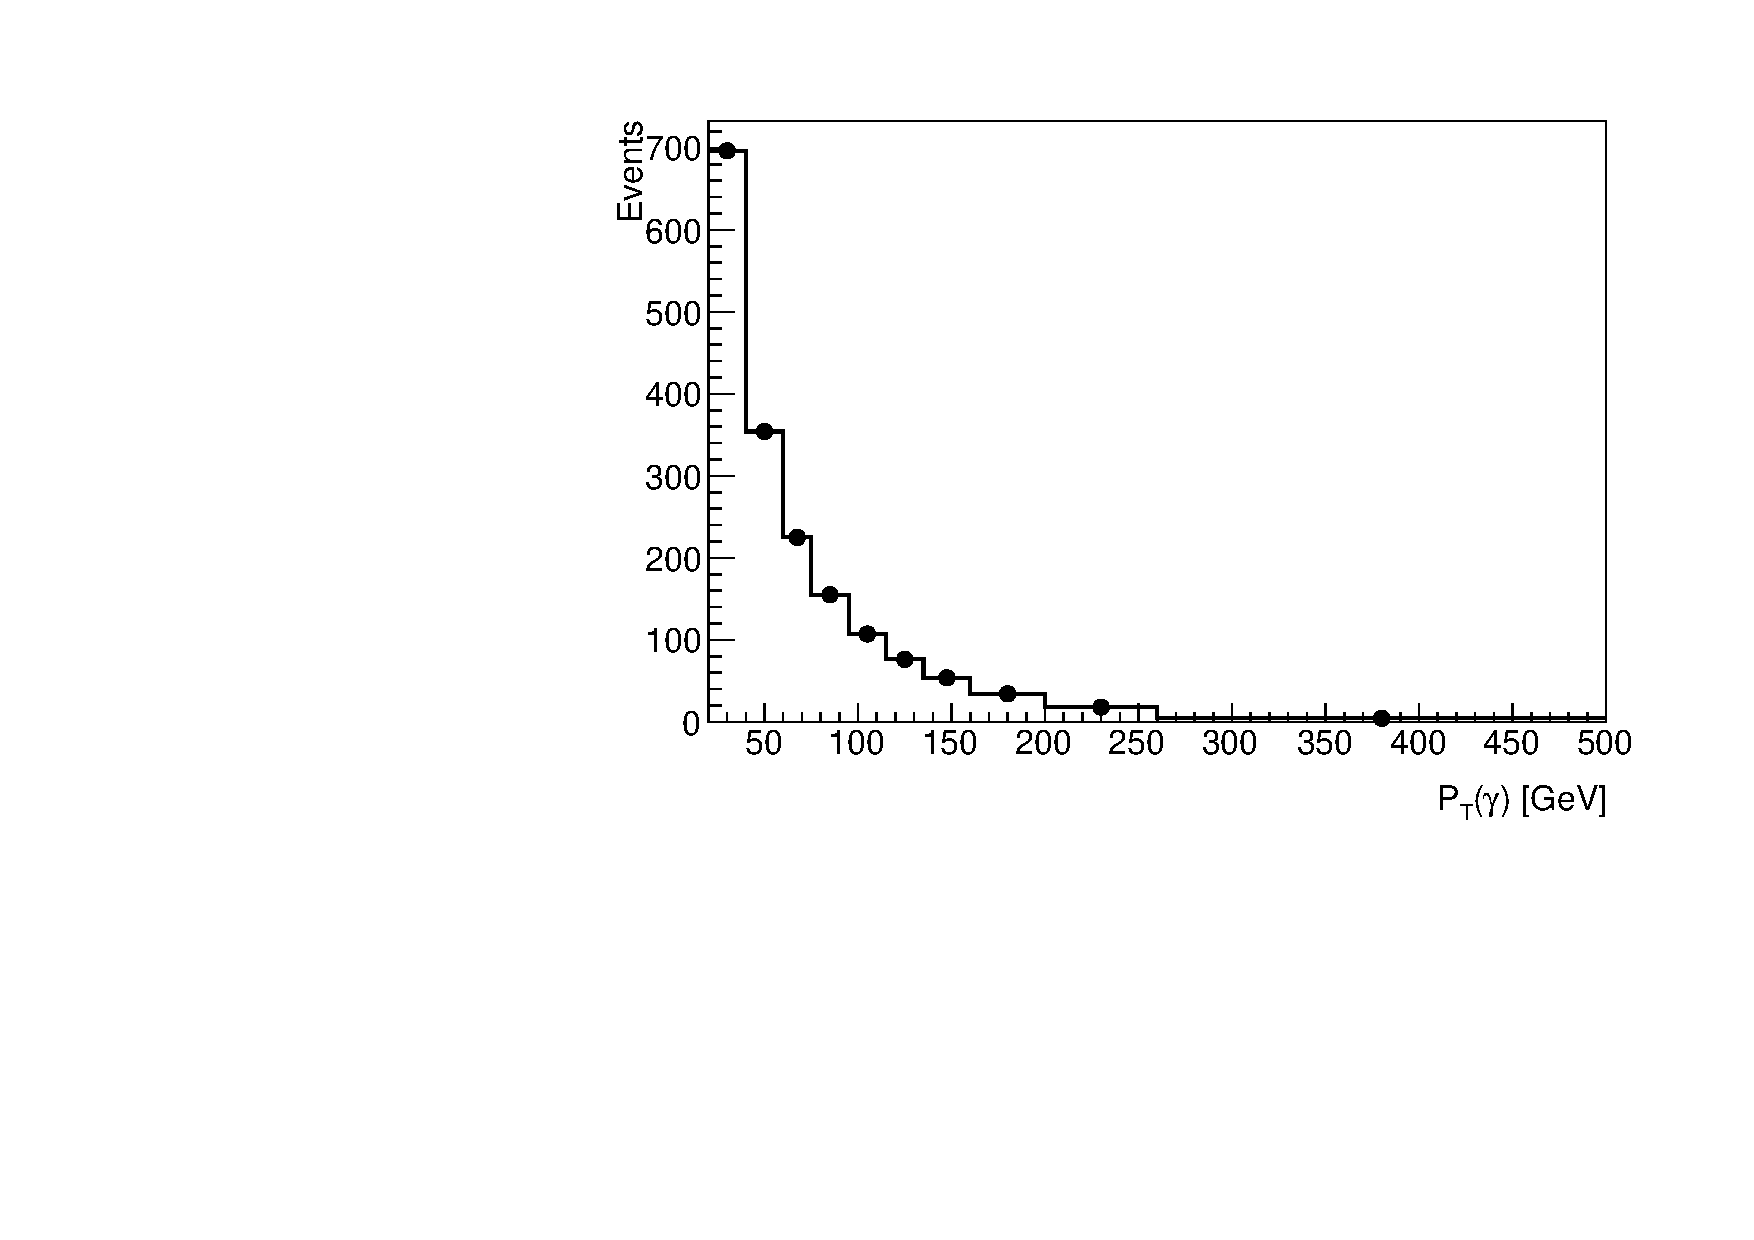
\includegraphics[width=0.3\textwidth]{figures/diff_xsec/ljet/Truth_dist/tty1l_pt_all_syst_Unfolding_truth_distribution.pdf}}
    \quad
    % ph eta
    \subfloat[]{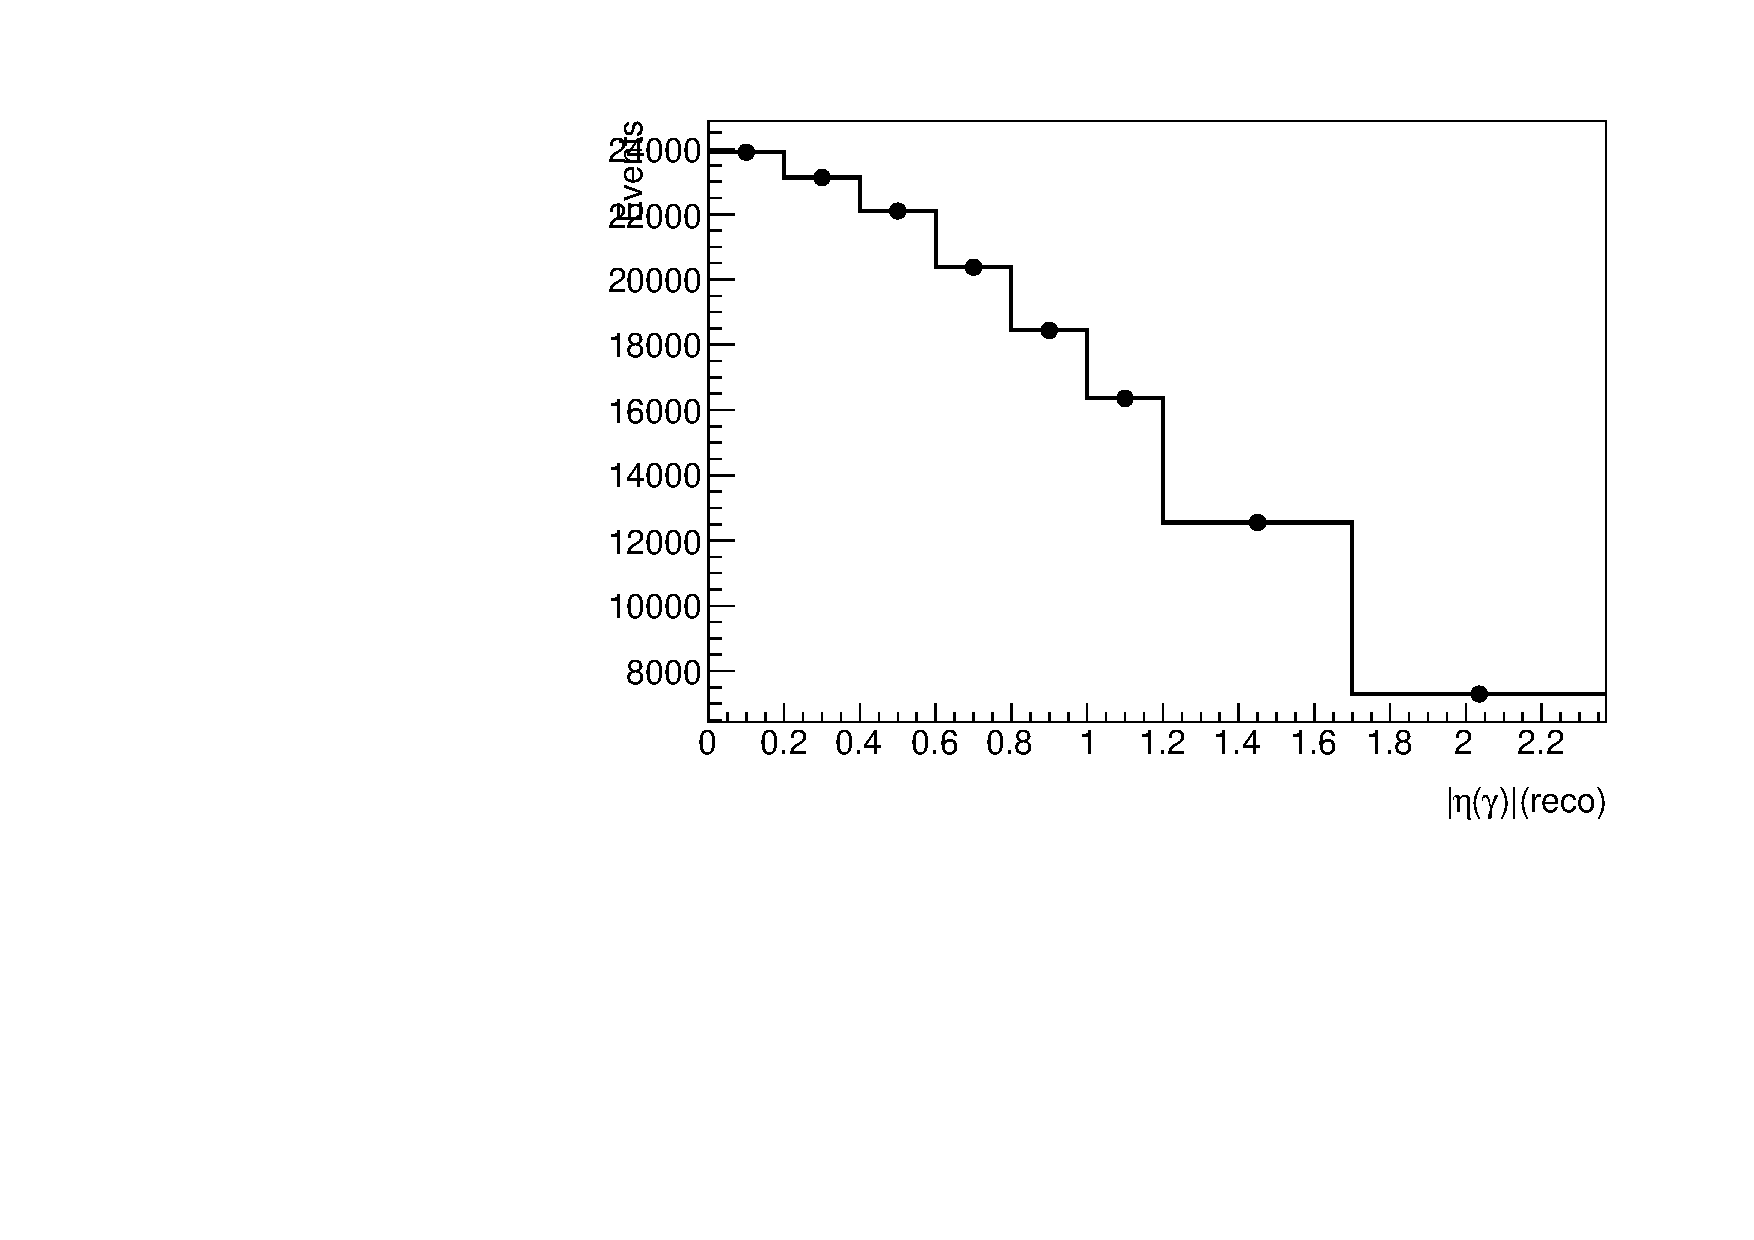
\includegraphics[width=0.3\textwidth]{figures/diff_xsec/ljet/Truth_dist/tty1l_eta_all_syst_Unfolding_truth_distribution.pdf}}
    \quad
    % delta R (ph, l)
    \subfloat[]{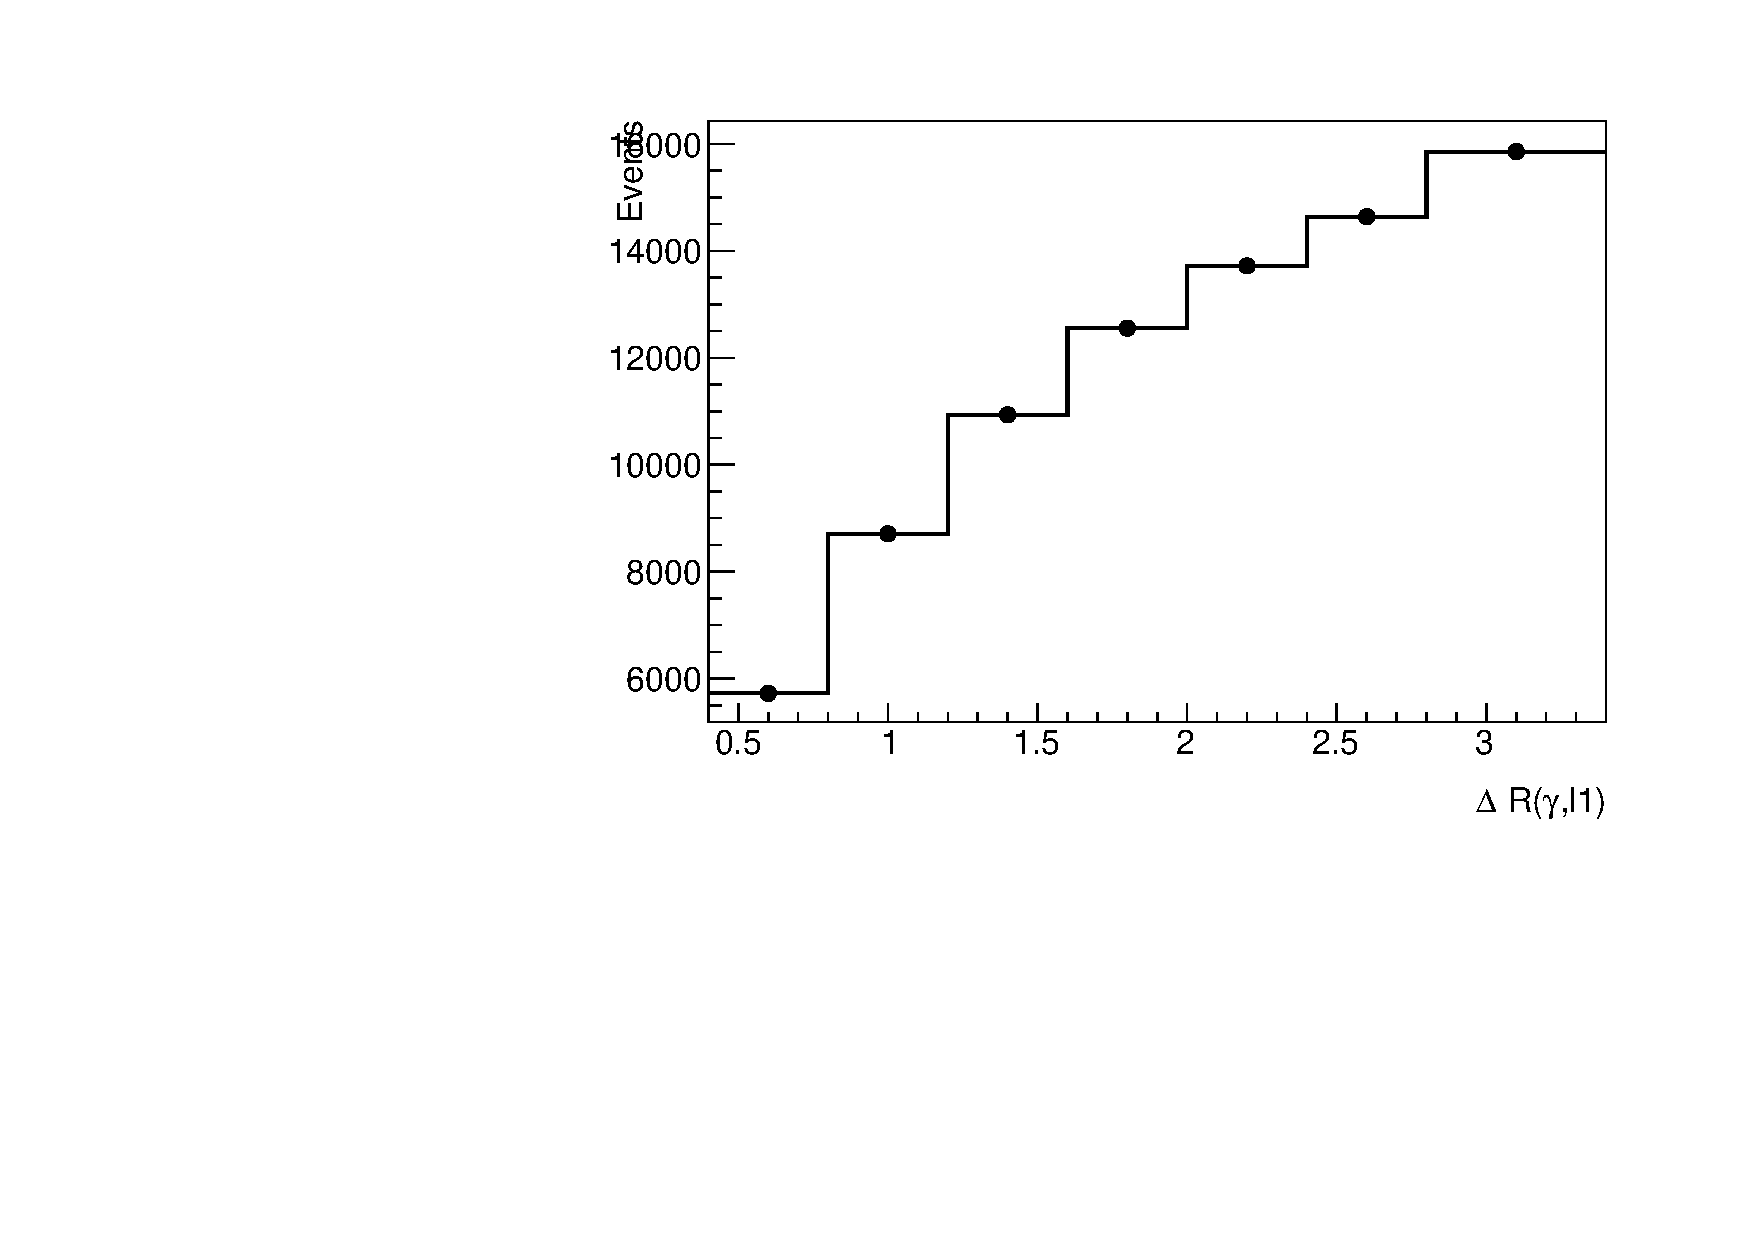
\includegraphics[width=0.3\textwidth]{figures/diff_xsec/ljet/Truth_dist/tty1l_dr_all_syst_Unfolding_truth_distribution.pdf}}
    \quad
    % delta R (ph, b)
    \subfloat[]{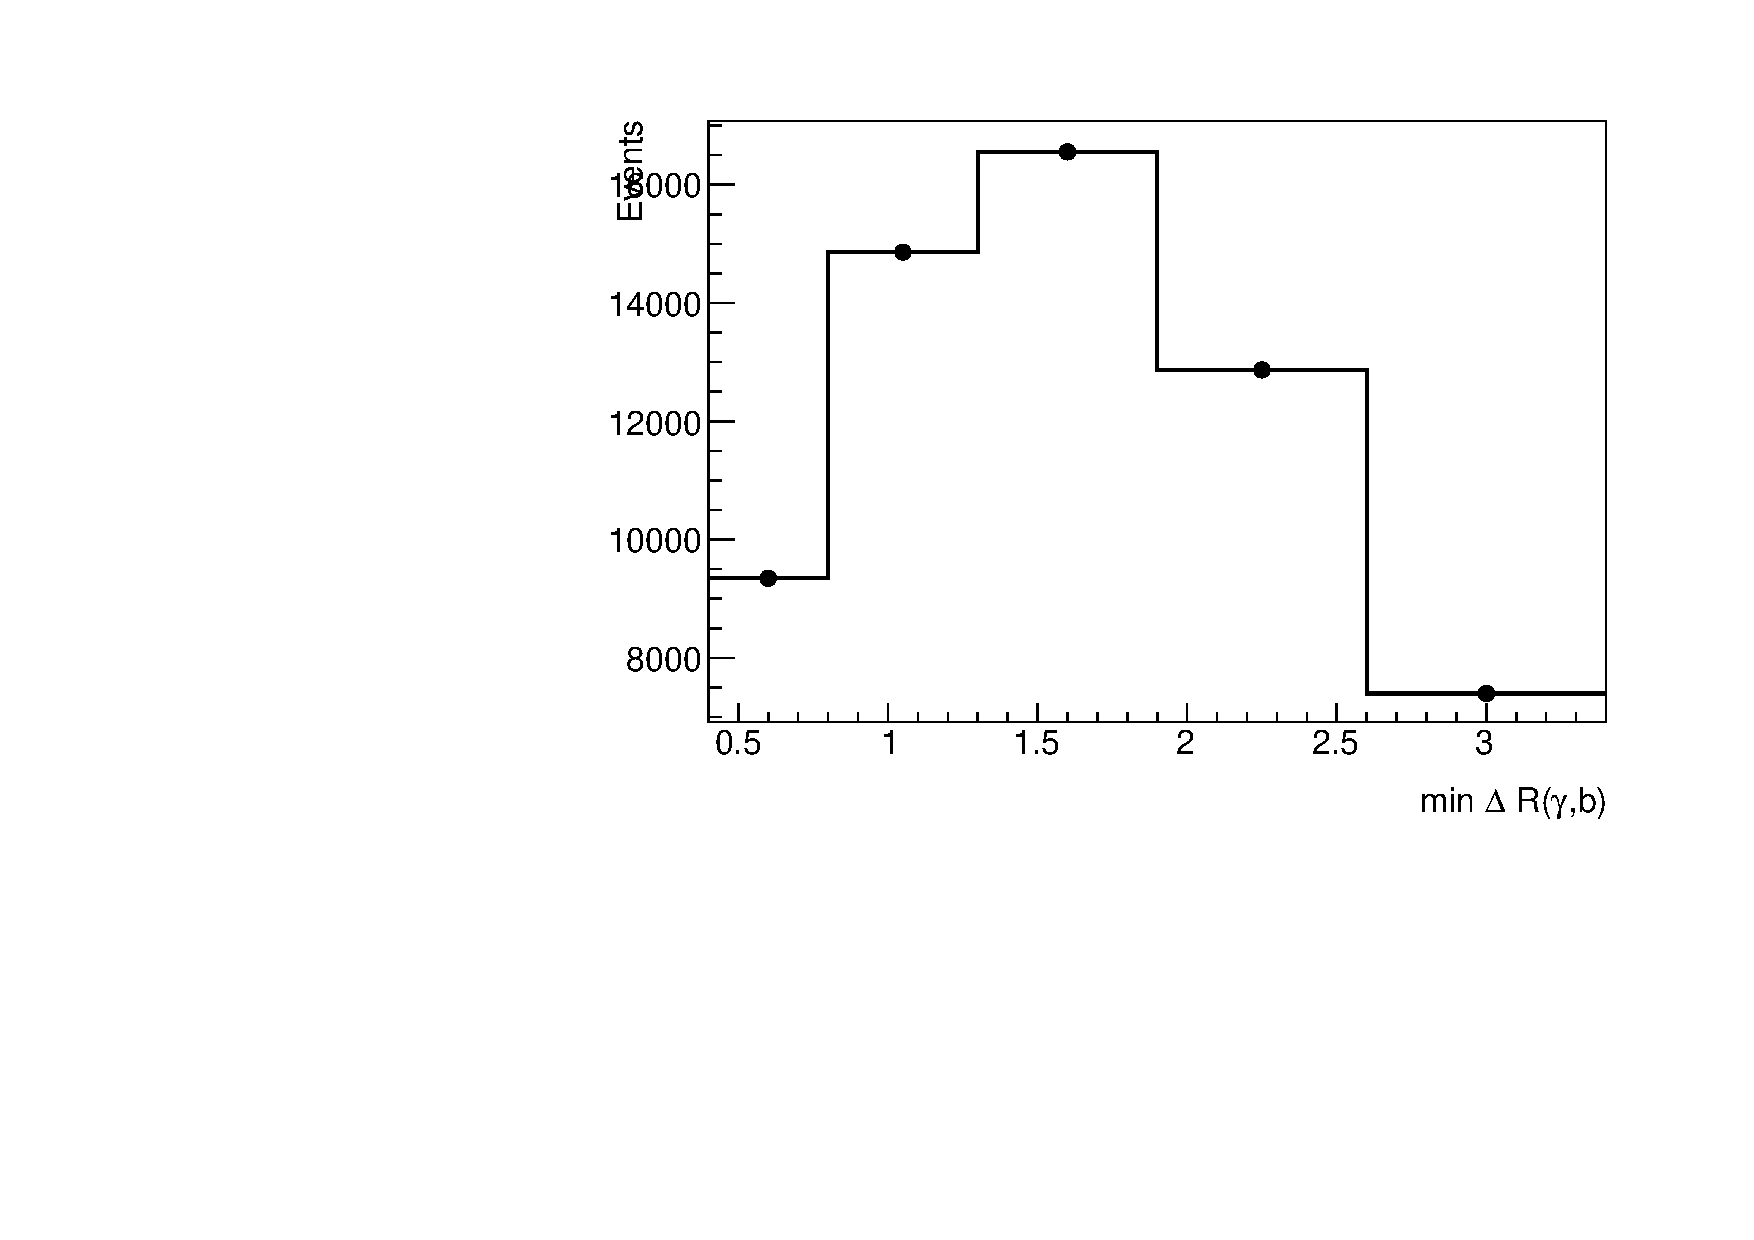
\includegraphics[width=0.3\textwidth]{figures/diff_xsec/ljet/Truth_dist/tty1l_drphb_all_syst_Unfolding_truth_distribution.pdf}}
    \quad
    % delta R(lj)
    \subfloat[]{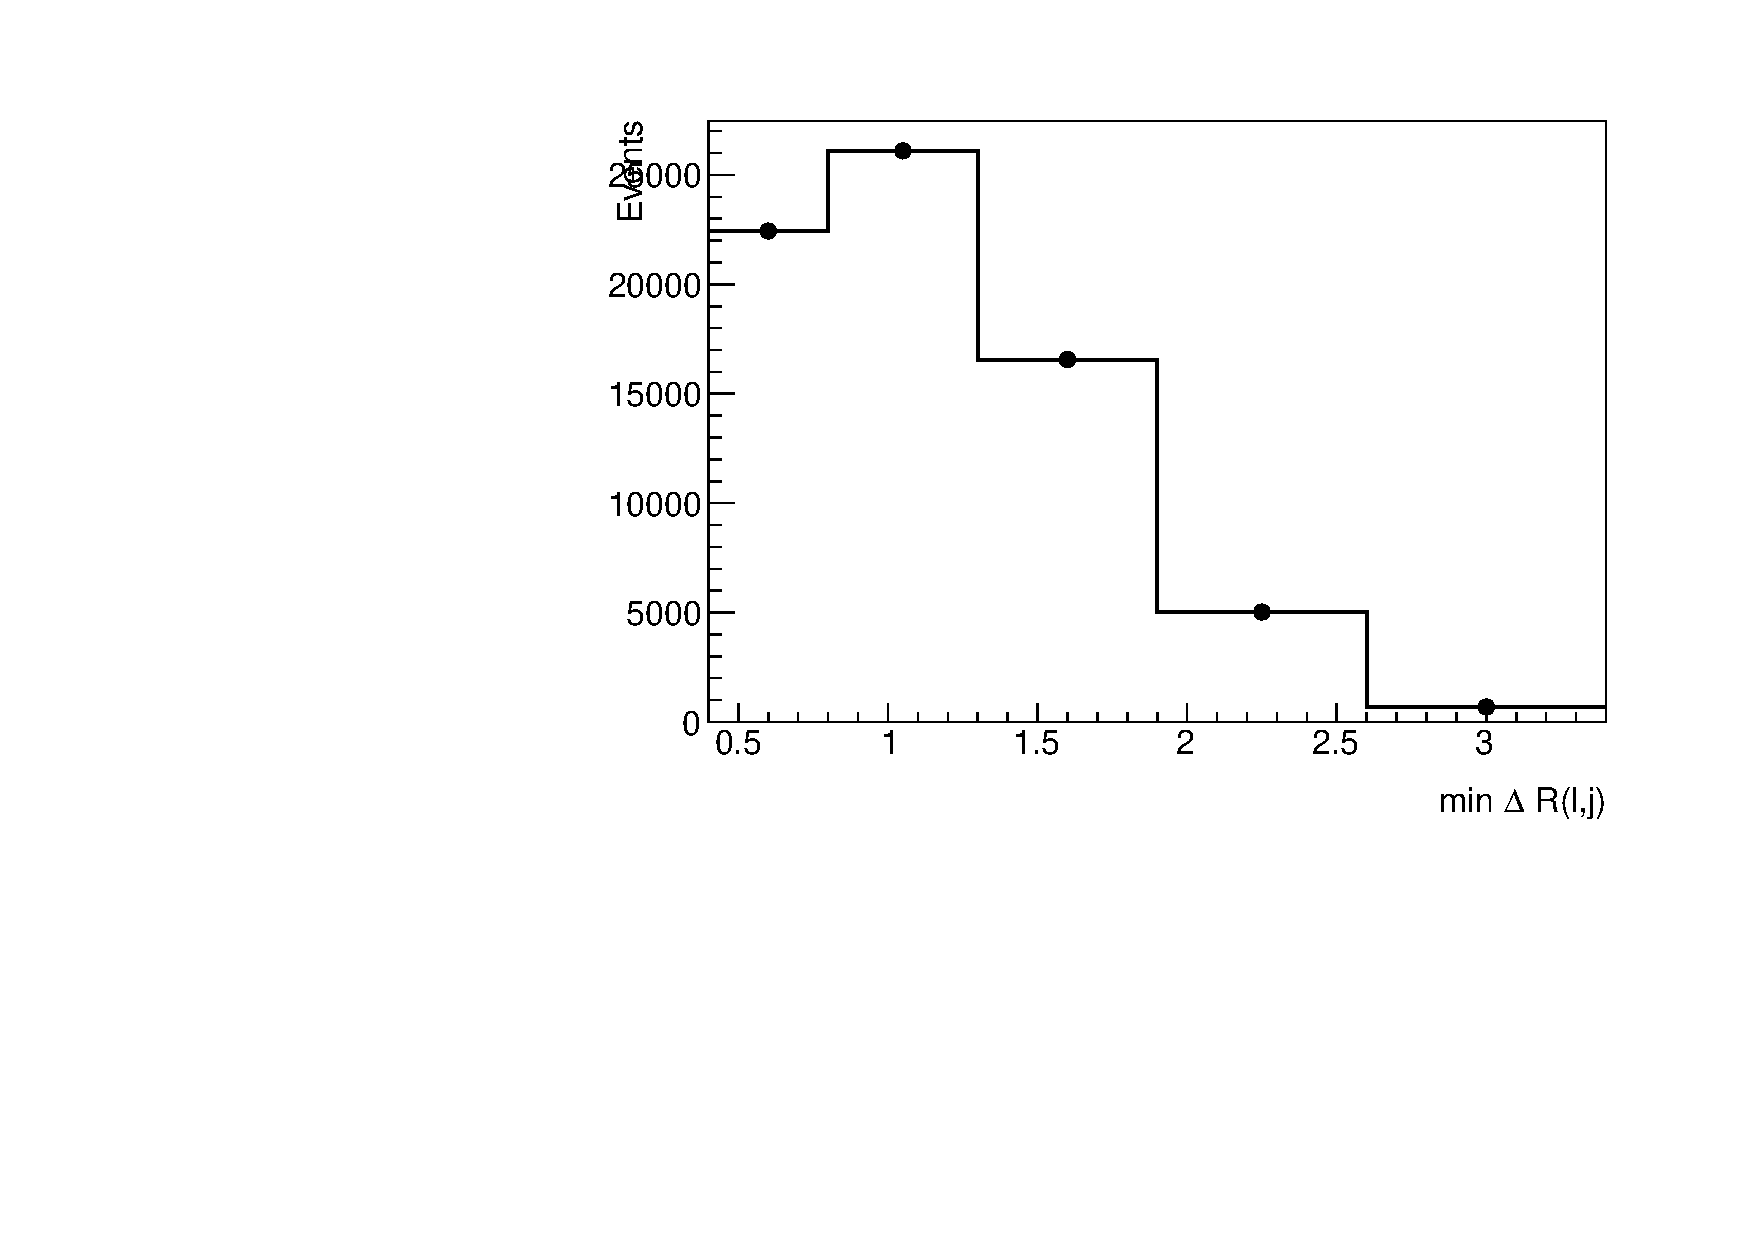
\includegraphics[width=0.3\textwidth]{figures/diff_xsec/ljet/Truth_dist/tty1l_drlj_all_syst_Unfolding_truth_distribution.pdf}}
    % pt j1
    \subfloat[]{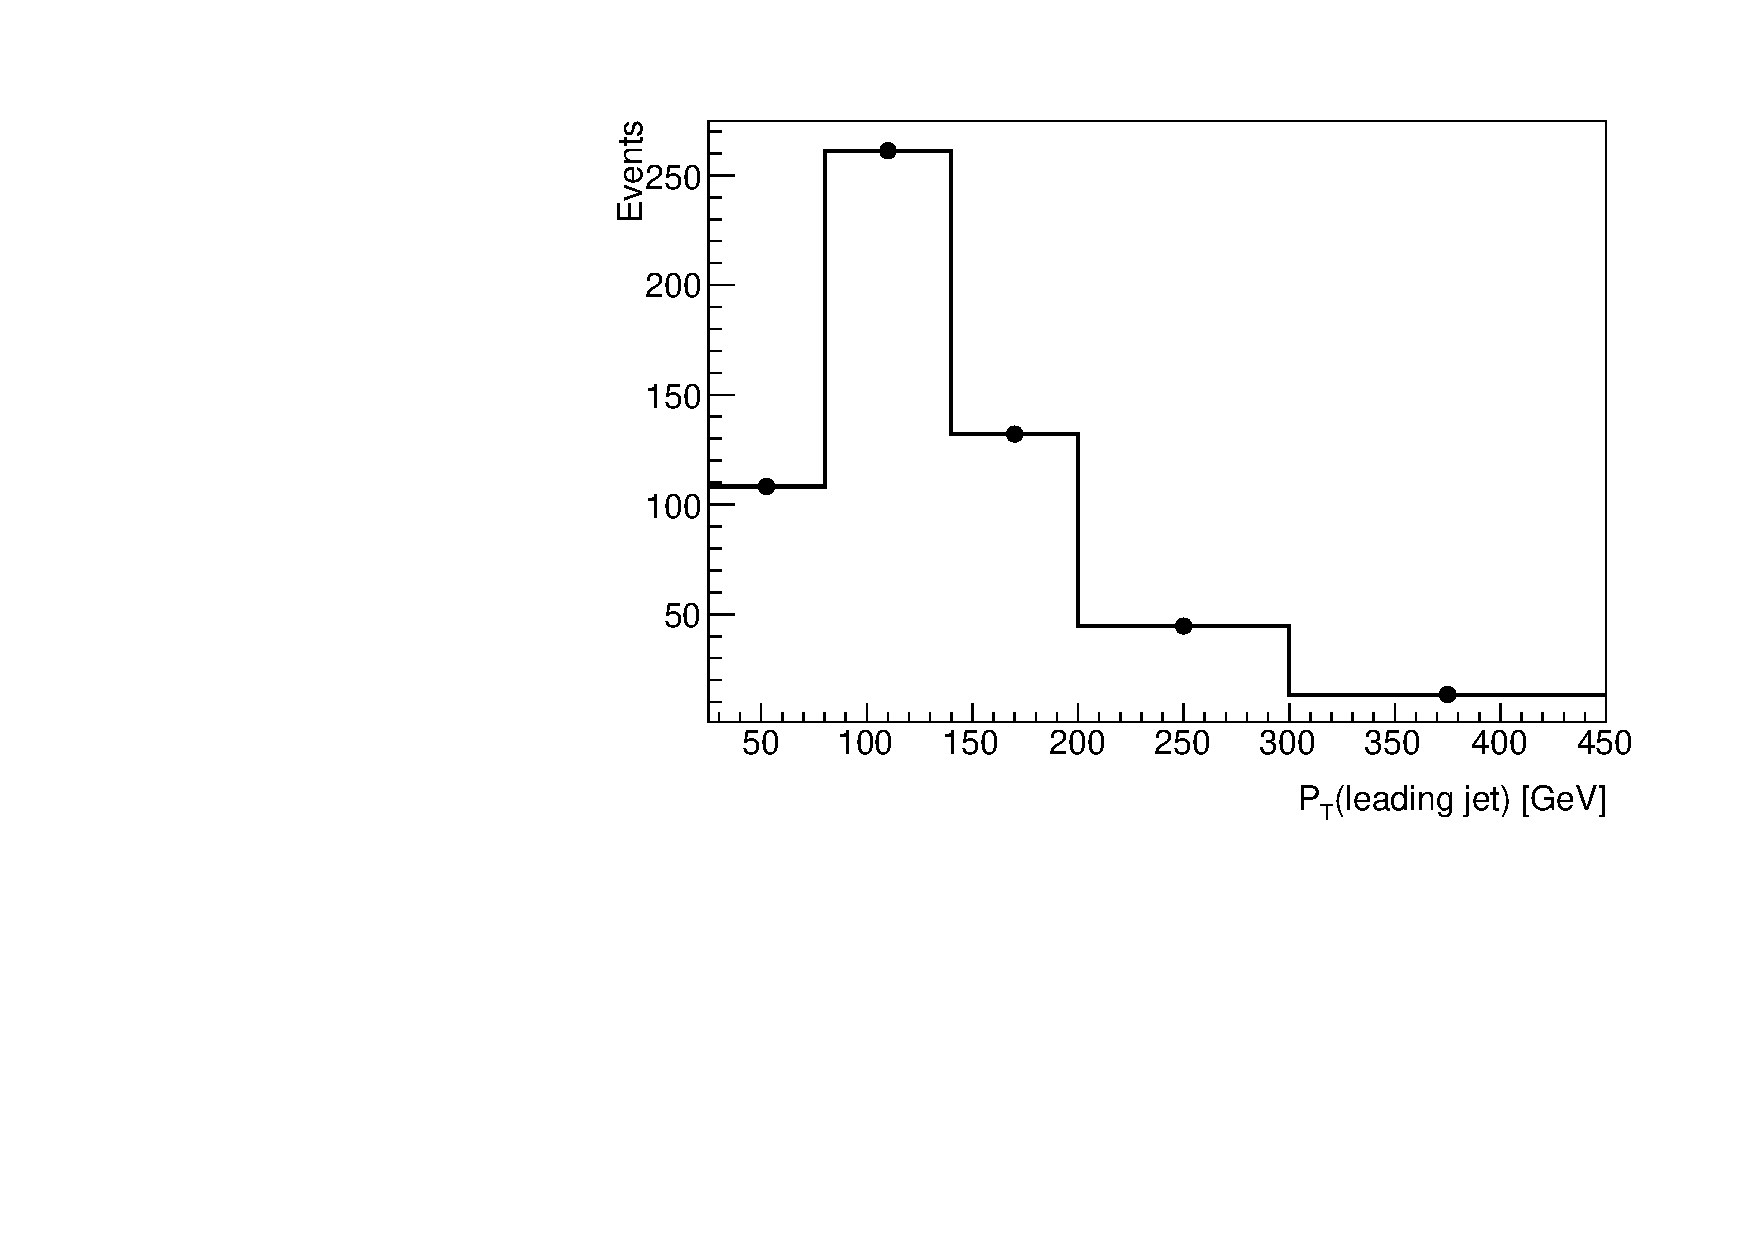
\includegraphics[width=0.3\textwidth]{figures/diff_xsec/ljet/Truth_dist/tty1l_ptj1_all_syst_Unfolding_truth_distribution.pdf}}
    \caption{The particle level distribution of \tty production as a function of different observables in the single-lepton channel. The number of events corresponds to the expected number of events at the particle level normalized to the luminosity of data. Overflow events are included in the last bin of the corresponding distribution. Note that values are divided by bin width.}
    \label{fig:folding_input_ljet}
\end{figure}
\FloatBarrier

\begin{figure}[ht]
    \centering
    % ph pt
    \subfloat[]{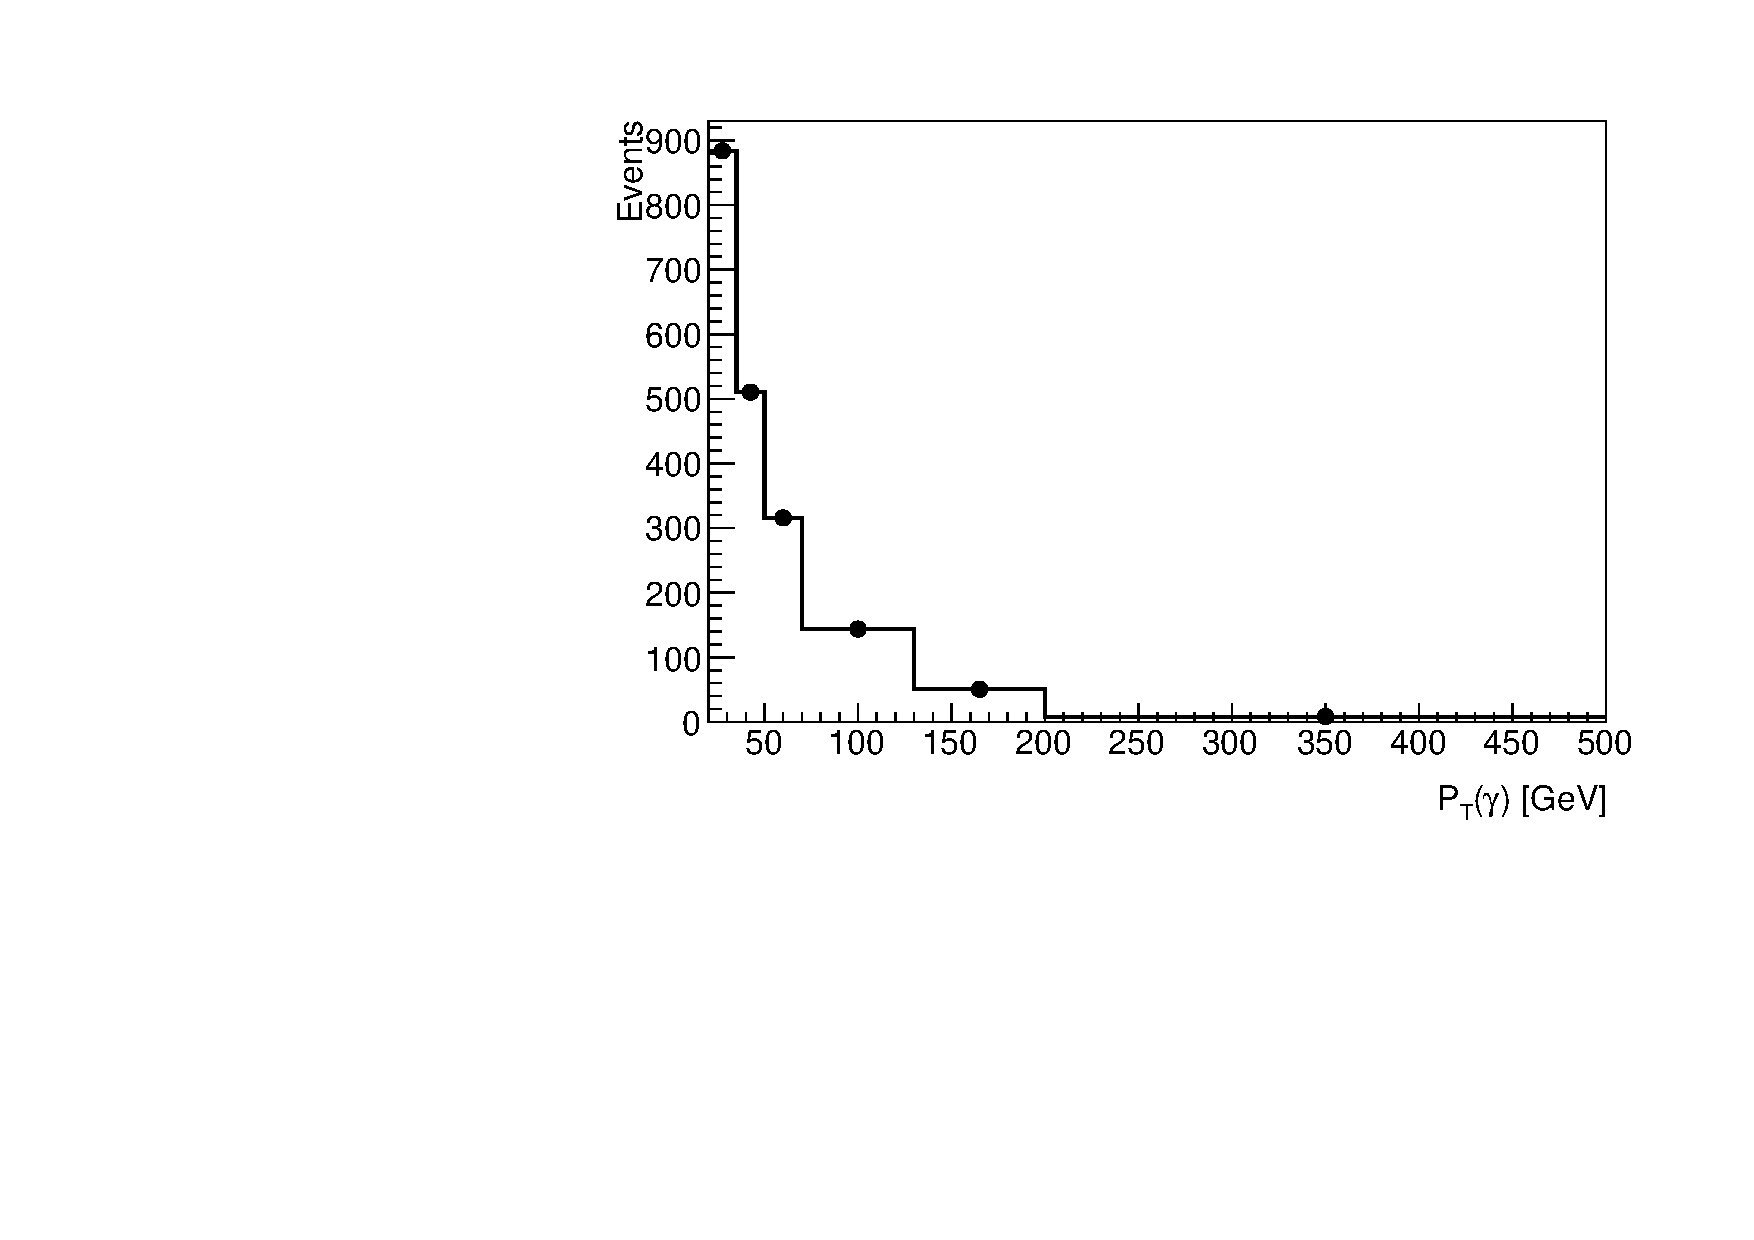
\includegraphics[width=0.3\textwidth]{figures/diff_xsec/dilep/Truth_dist/tty2l_pt_all_syst_Unfolding_truth_distribution.pdf}}
    \quad
    % ph eta
    \subfloat[]{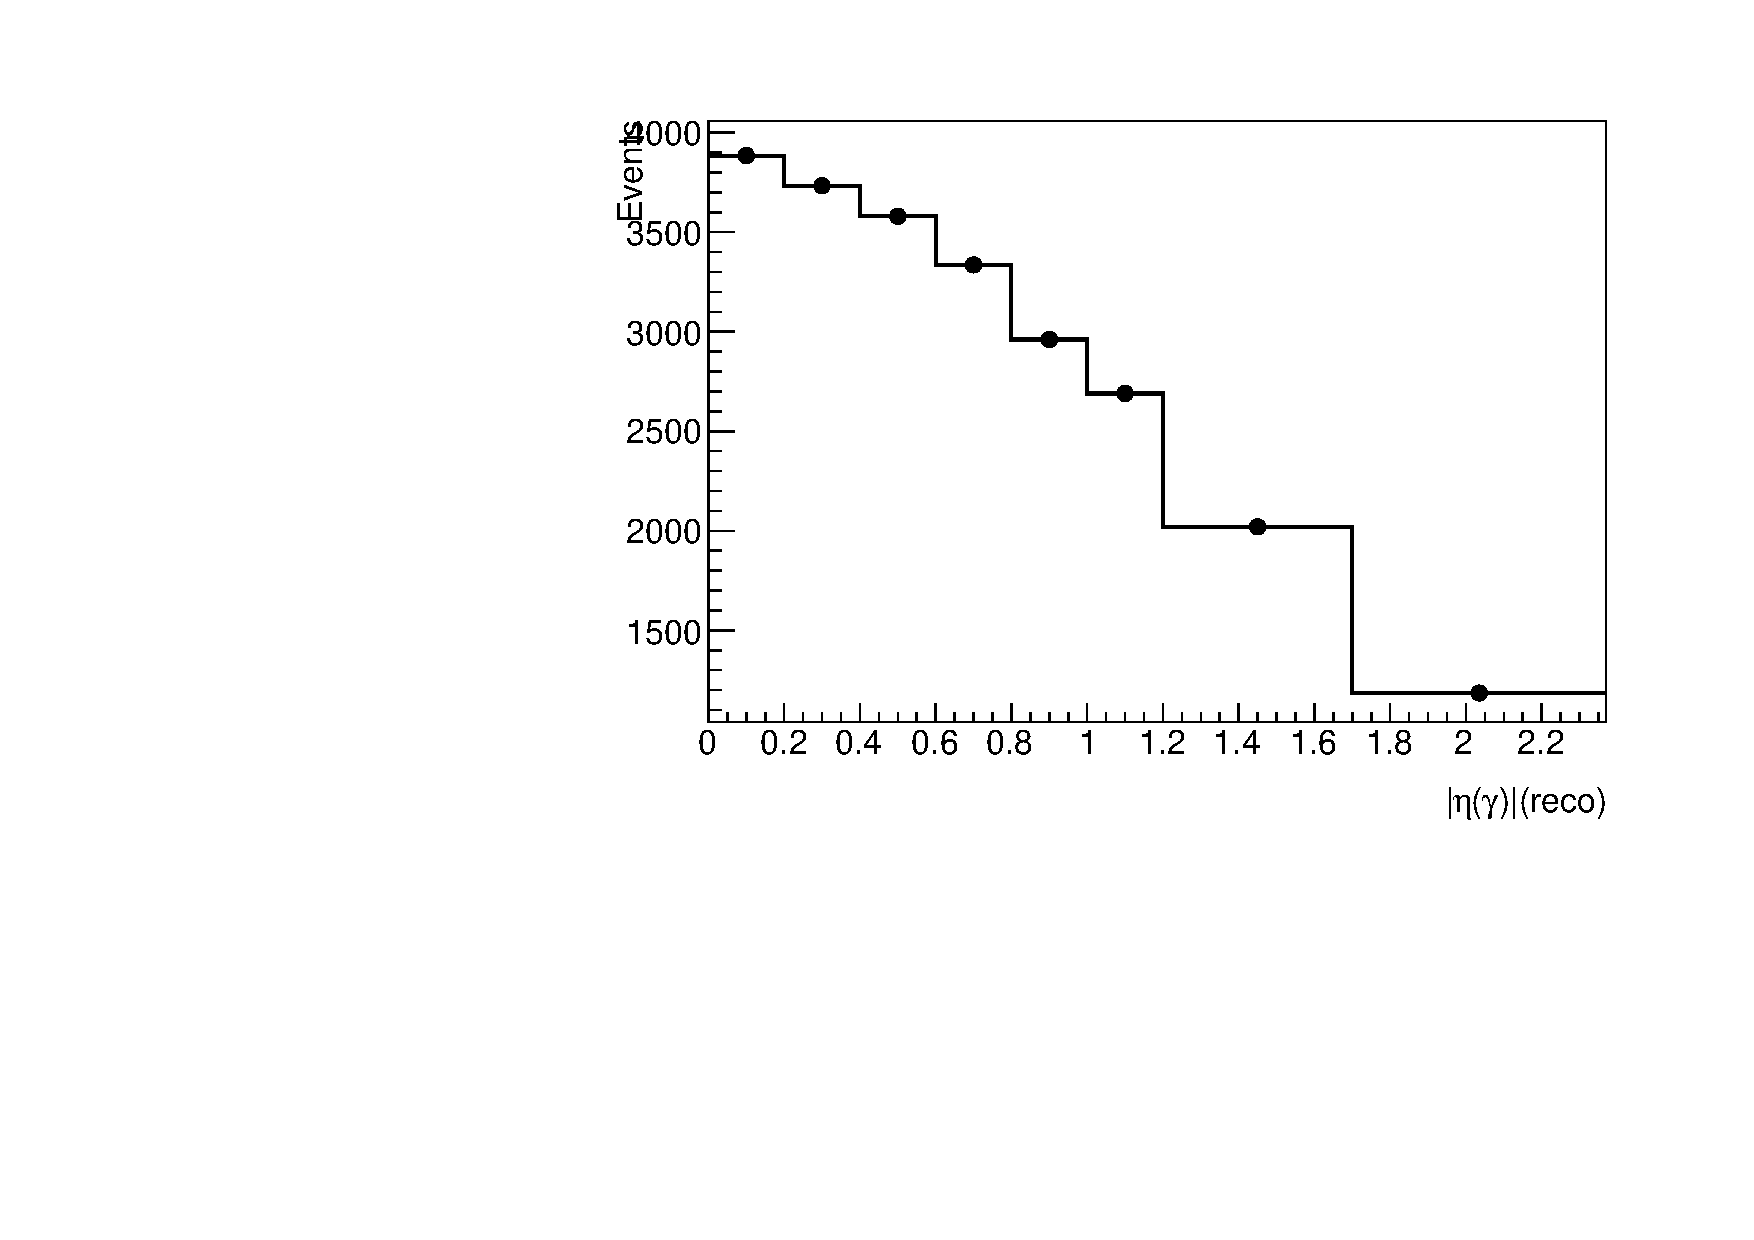
\includegraphics[width=0.3\textwidth]{figures/diff_xsec/dilep/Truth_dist/tty2l_eta_all_syst_Unfolding_truth_distribution.pdf}}
    \quad
    % delta R (ph, l)
    \subfloat[]{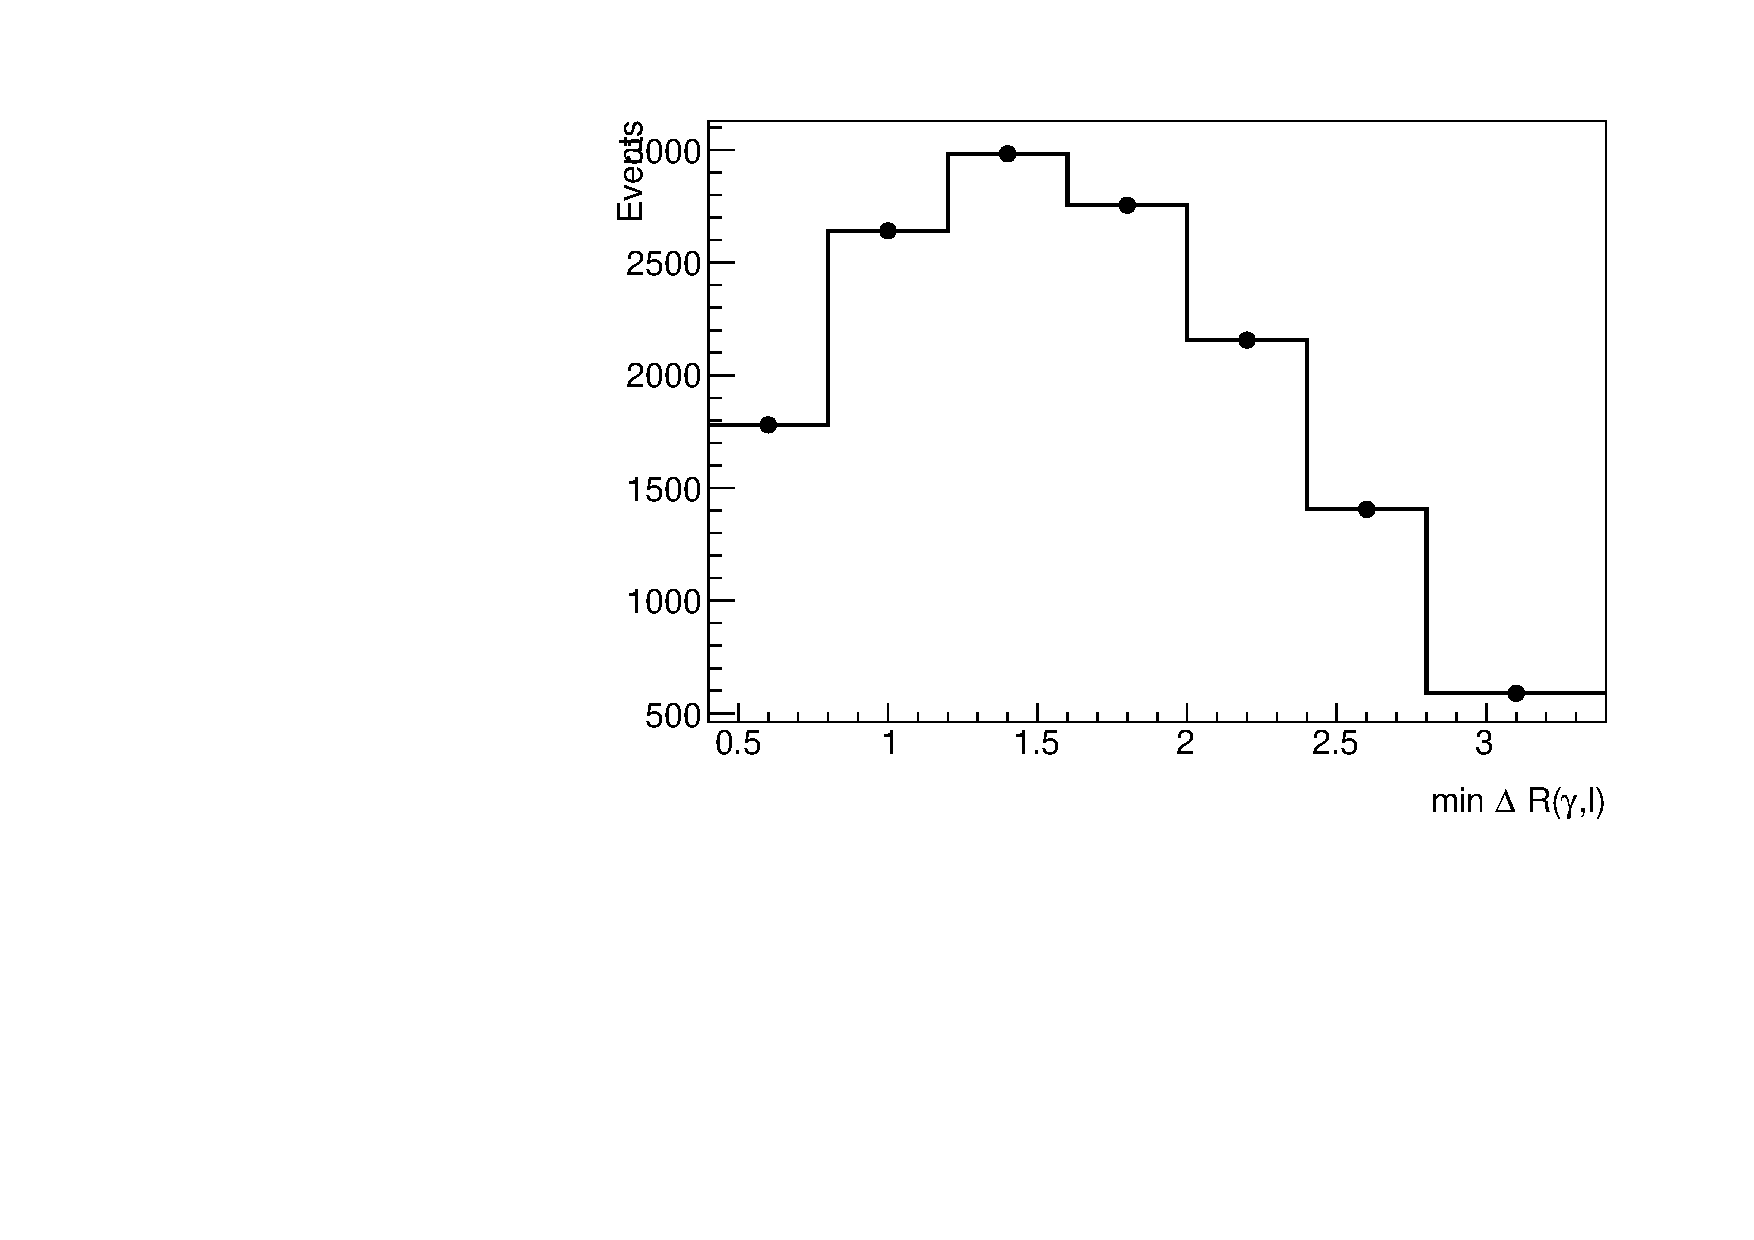
\includegraphics[width=0.3\textwidth]{figures/diff_xsec/dilep/Truth_dist/tty2l_dr_all_syst_Unfolding_truth_distribution.pdf}}
    \quad
    % delta R (ph, l1)
    \subfloat[]{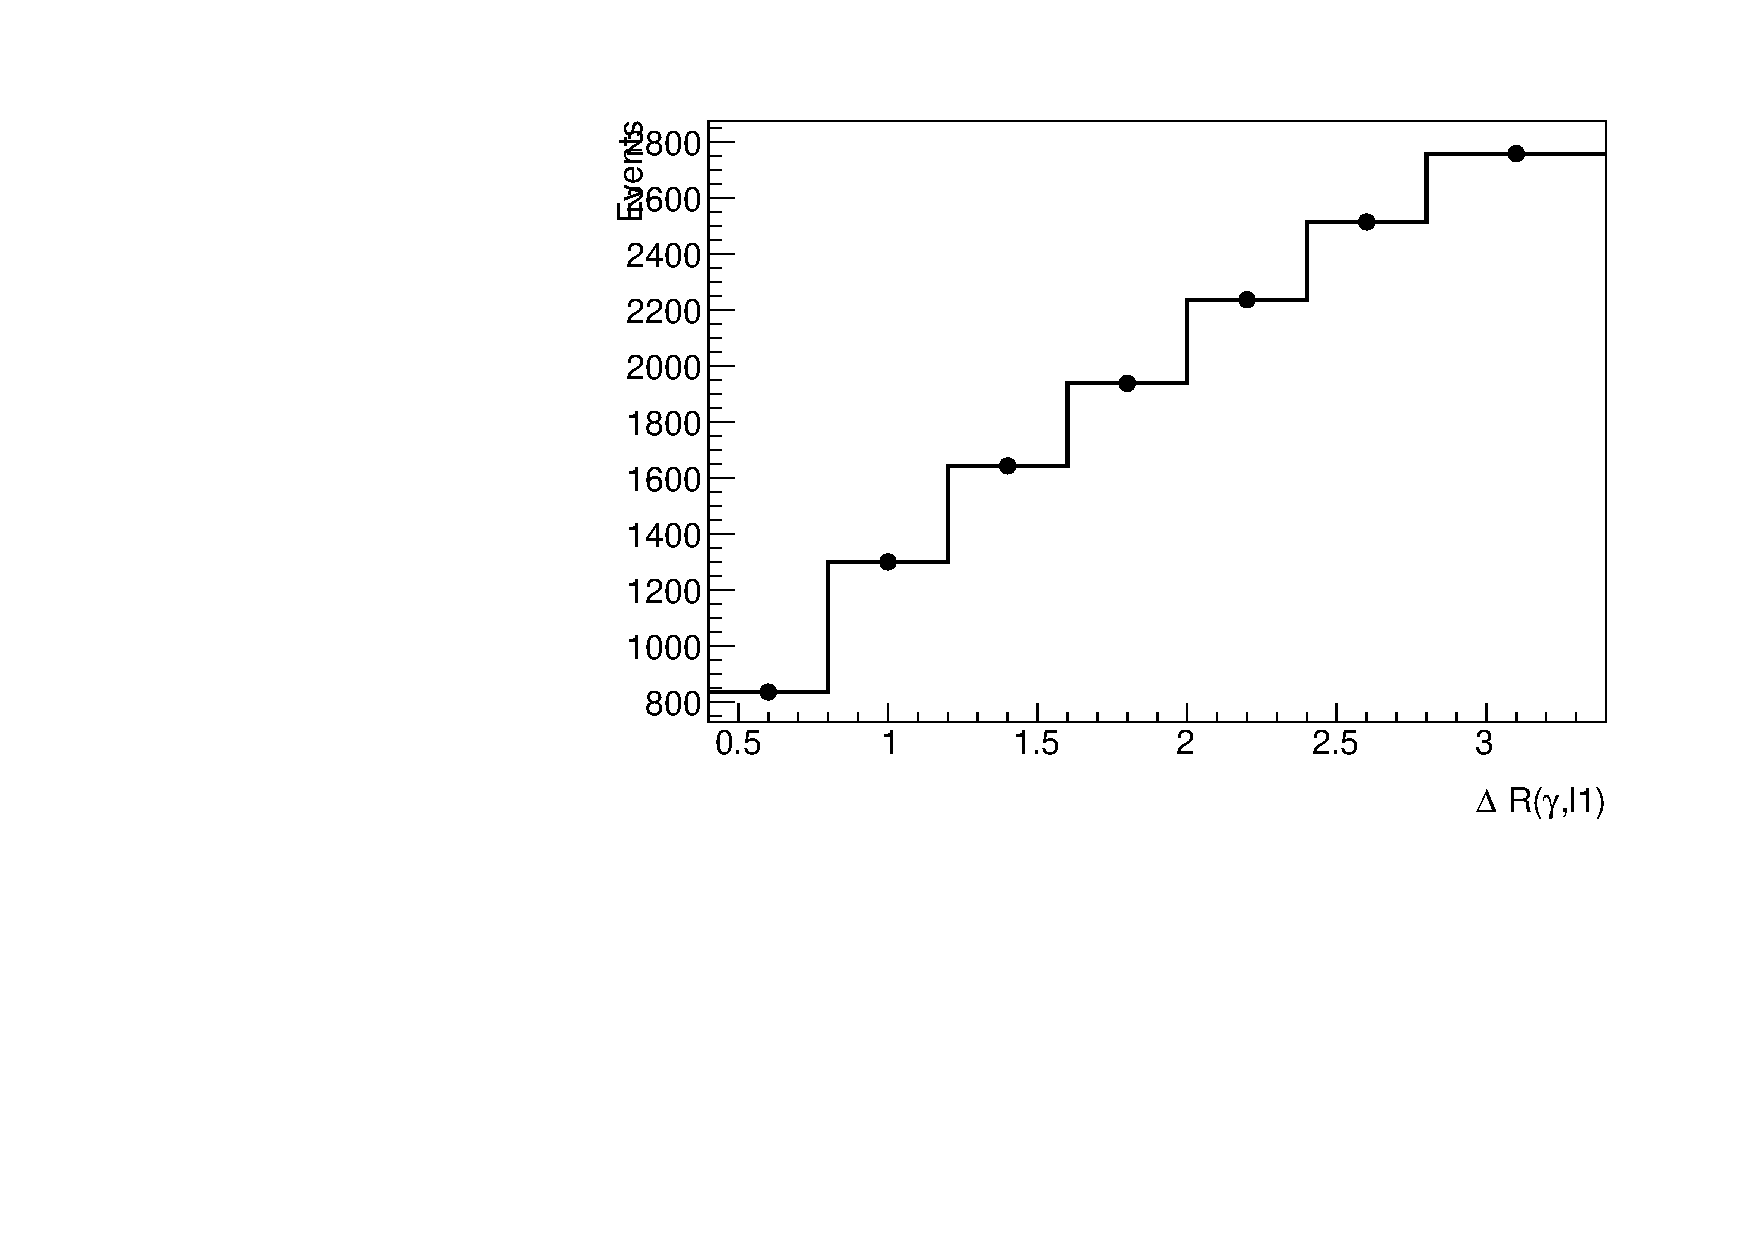
\includegraphics[width=0.3\textwidth]{figures/diff_xsec/dilep/Truth_dist/tty2l_dr1_all_syst_Unfolding_truth_distribution.pdf}}
    \quad
    % delta R (ph, l2)
    \subfloat[]{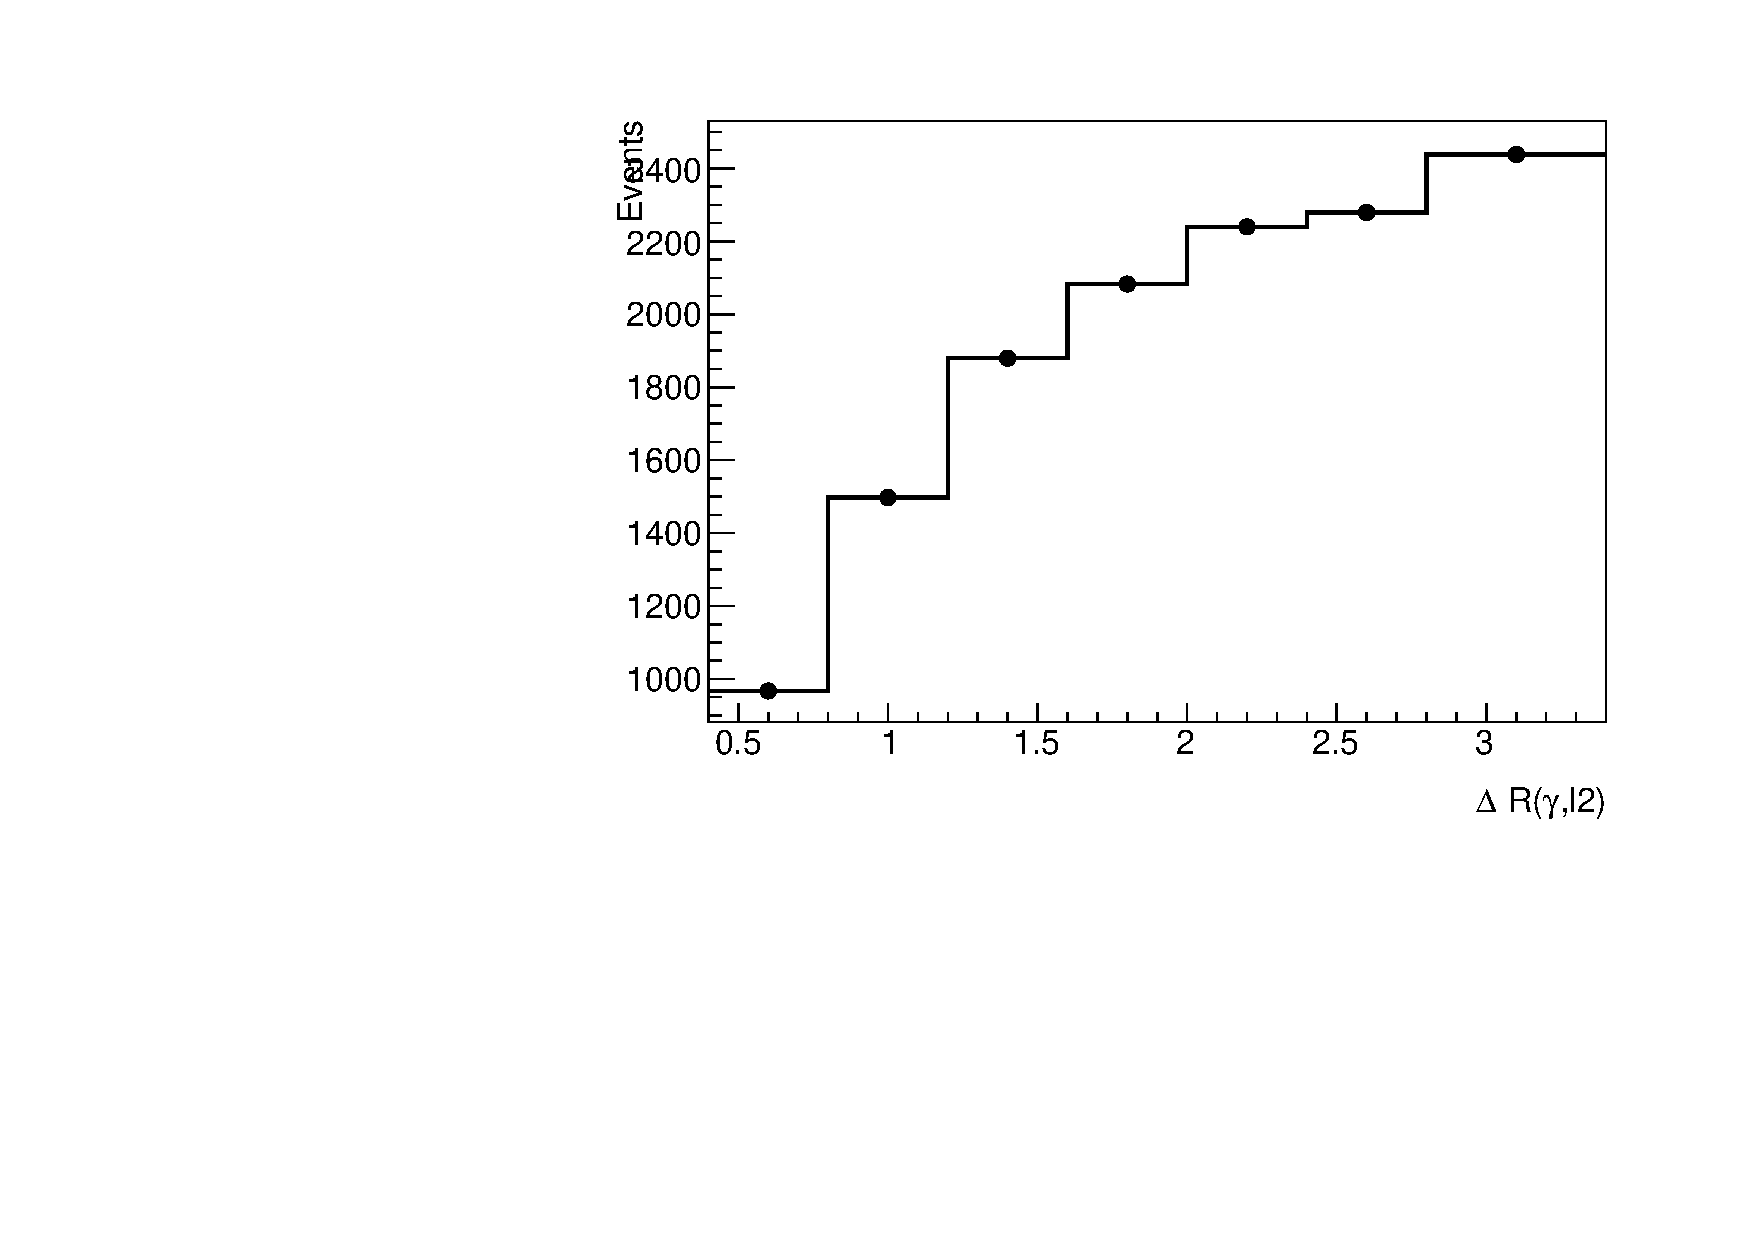
\includegraphics[width=0.3\textwidth]{figures/diff_xsec/dilep/Truth_dist/tty2l_dr2_all_syst_Unfolding_truth_distribution.pdf}}
    \quad
    % delta R (ph, b)
    \subfloat[]{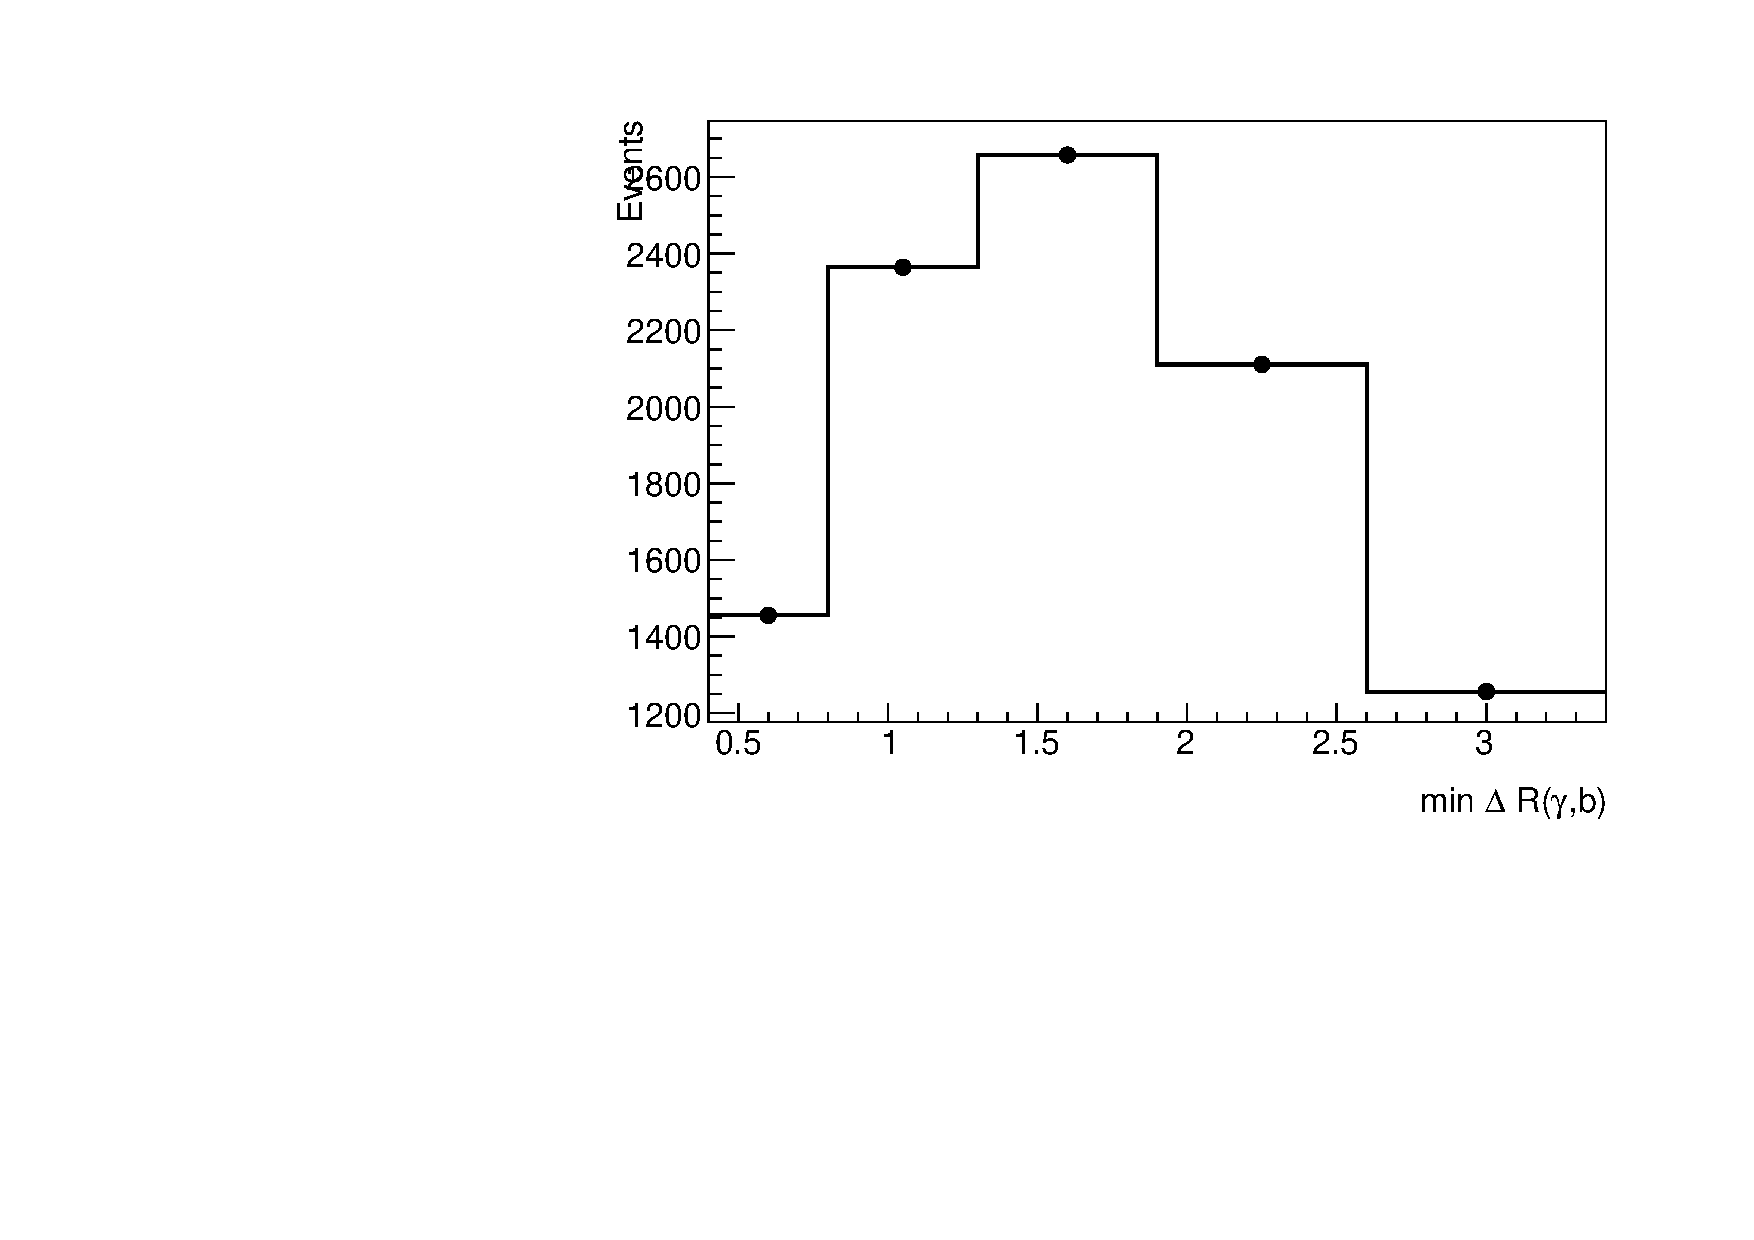
\includegraphics[width=0.3\textwidth]{figures/diff_xsec/dilep/Truth_dist/tty2l_drphb_all_syst_Unfolding_truth_distribution.pdf}}
    \quad
    % dEta(ll)
    \subfloat[]{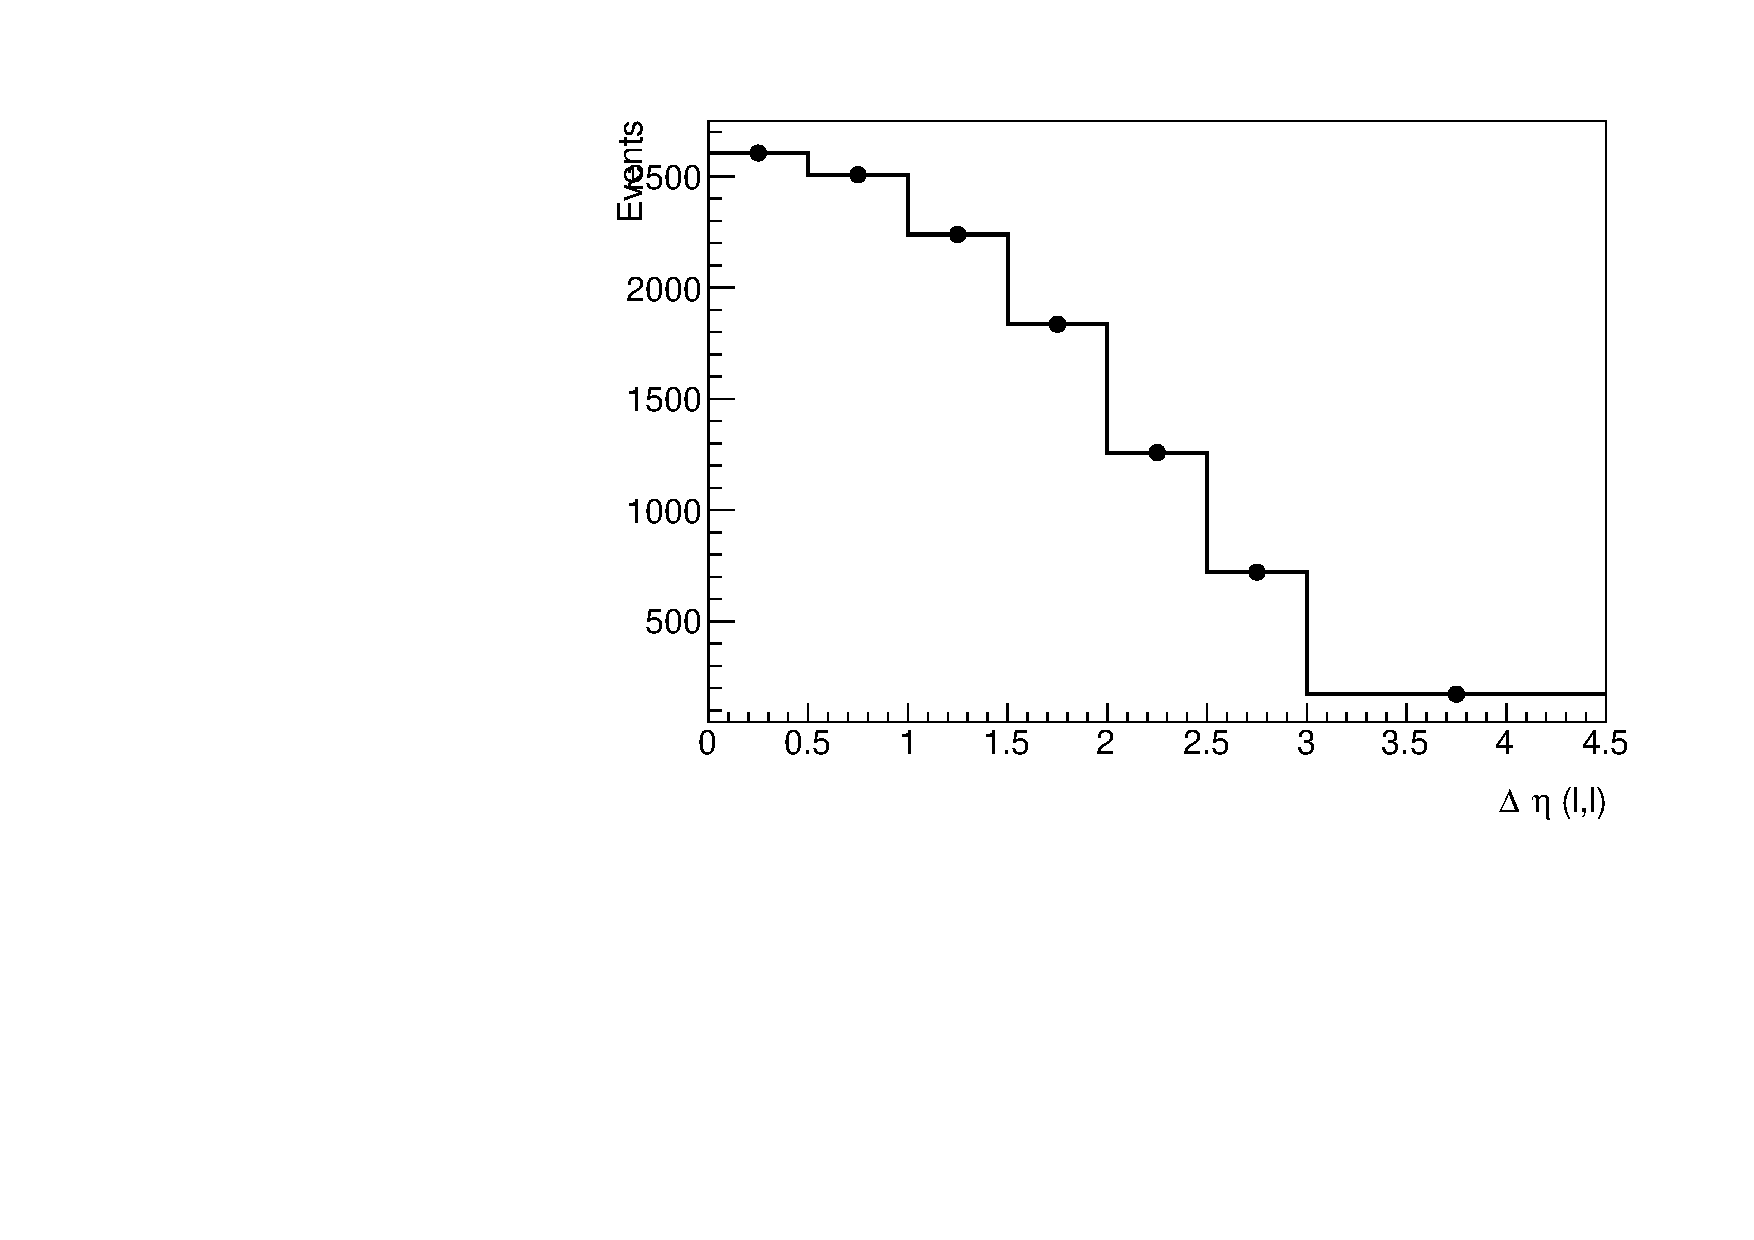
\includegraphics[width=0.3\textwidth]{figures/diff_xsec/dilep/Truth_dist/tty2l_dEtall_all_syst_Unfolding_truth_distribution.pdf}}
    \quad
    % dPhi(ll)
    \subfloat[]{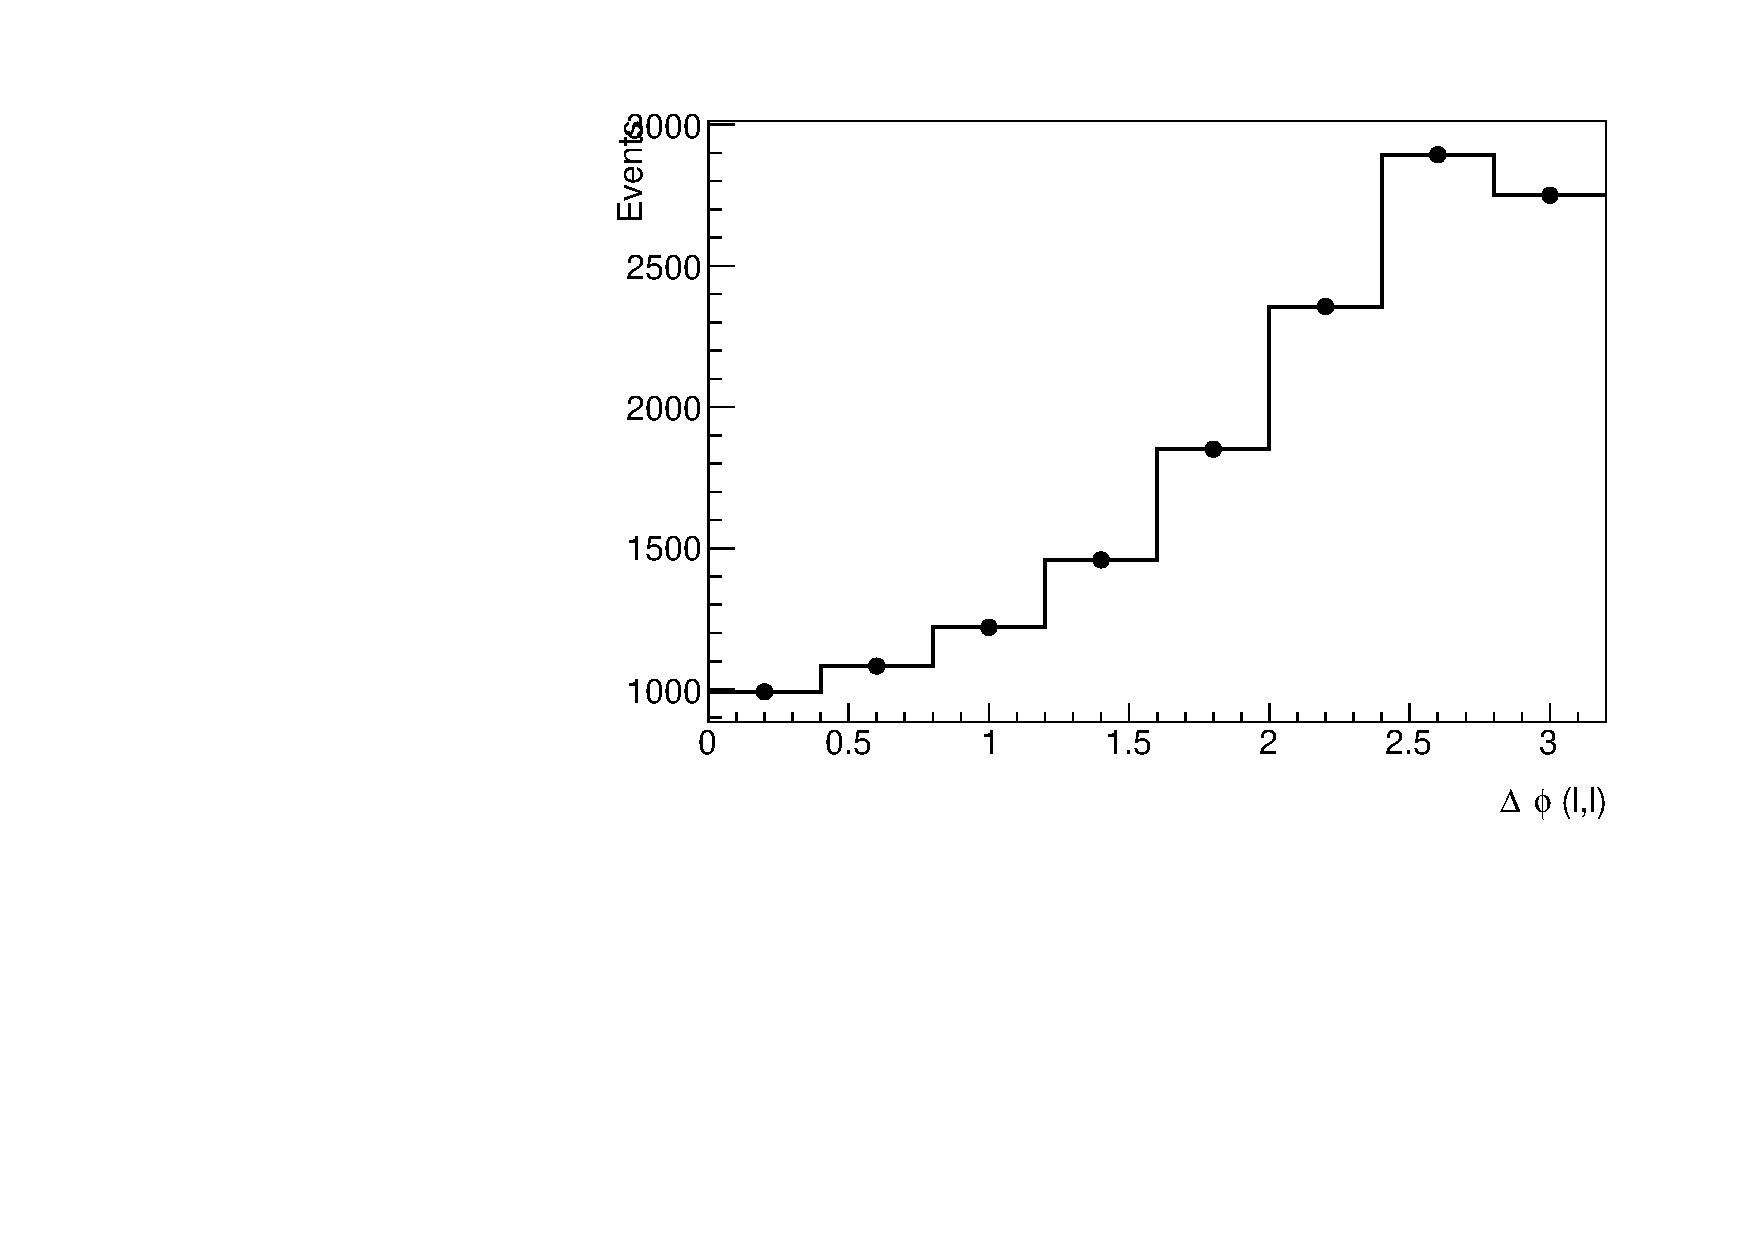
\includegraphics[width=0.3\textwidth]{figures/diff_xsec/dilep/Truth_dist/tty2l_dPhill_all_syst_Unfolding_truth_distribution.pdf}}
    \quad
    % Pt(ll)
    \subfloat[]{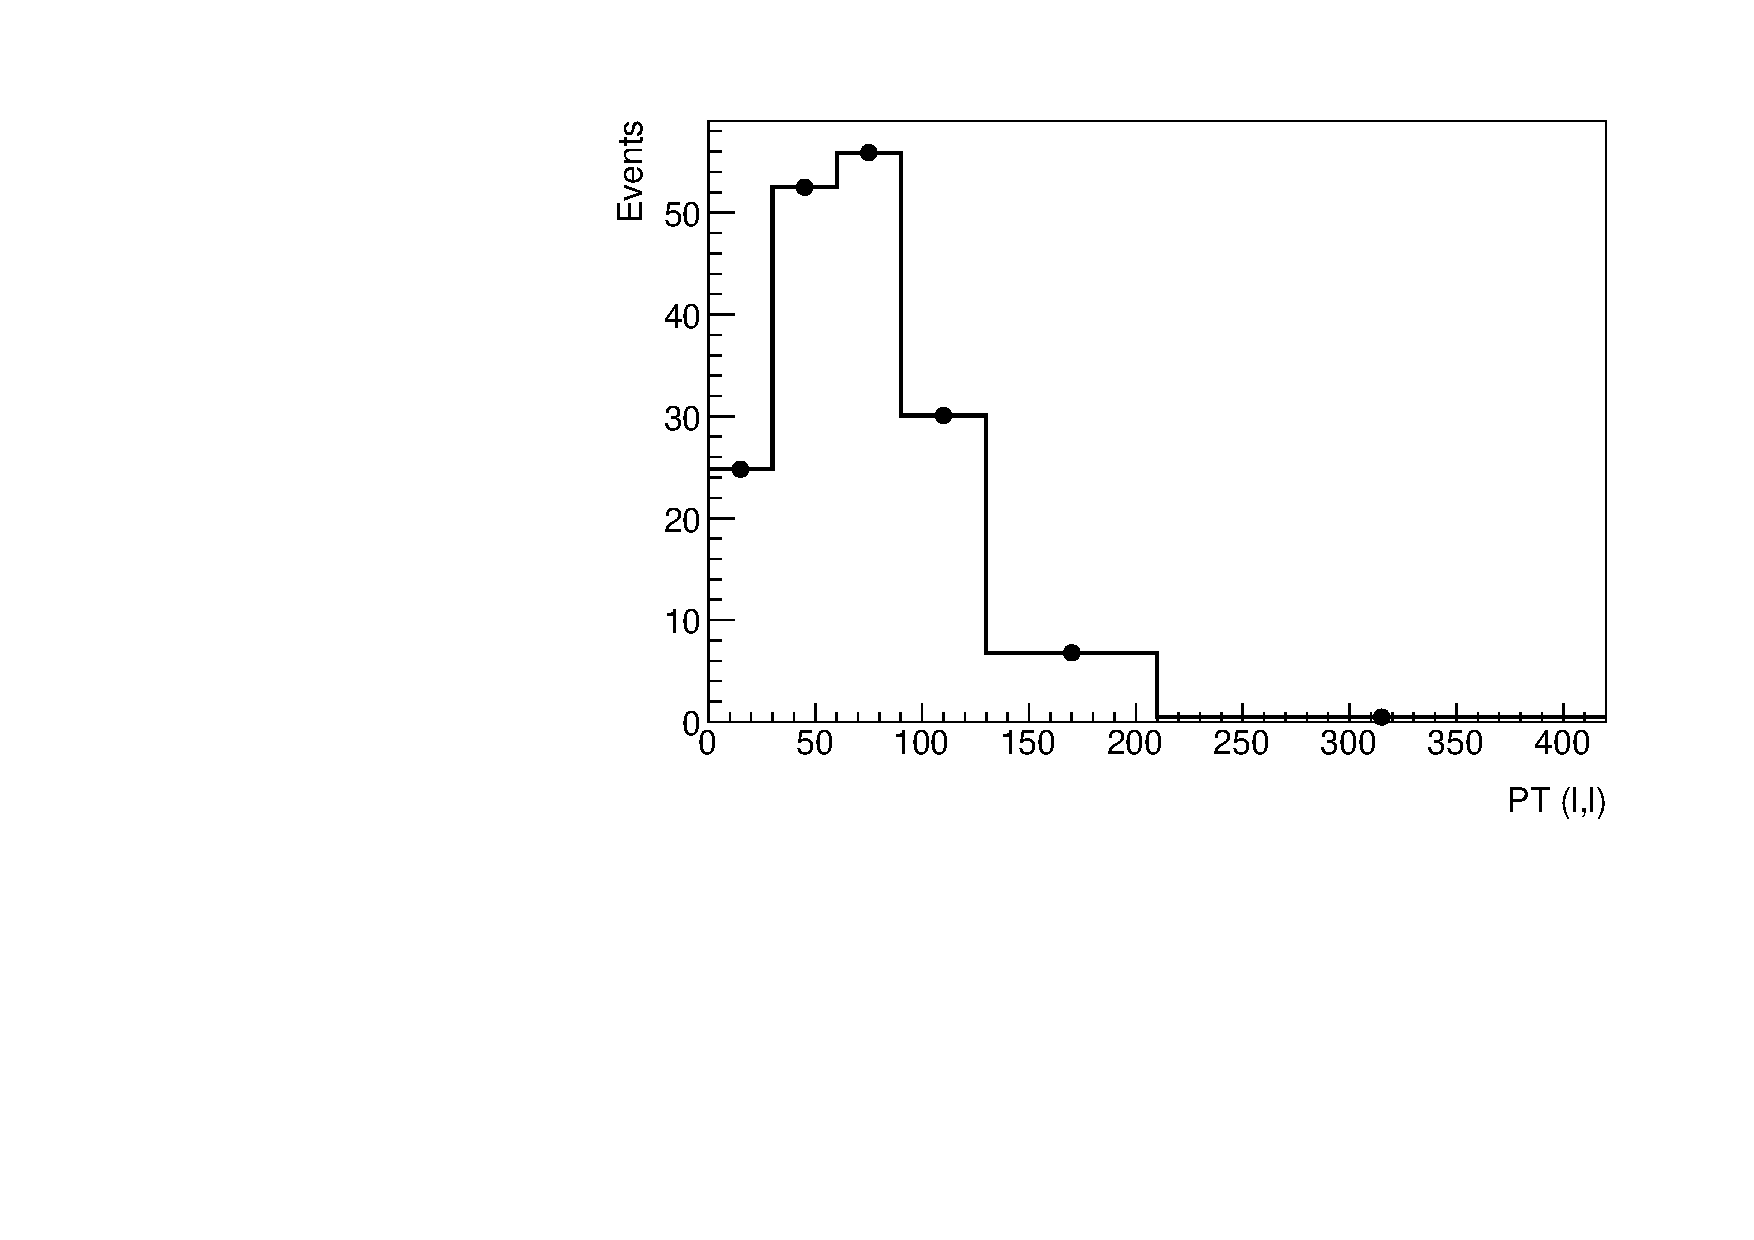
\includegraphics[width=0.3\textwidth]{figures/diff_xsec/dilep/Truth_dist/tty2l_ptll_all_syst_Unfolding_truth_distribution.pdf}}
    \quad
    % Delta R (lj)
    \subfloat[]{\includegraphics[width=0.3\textwidth]{figures/diff_xsec/dilep/Truth_dist/tty2l_drlj_all_syst_Unfolding_truth_distribution.pdf}}
    \quad
    % pt j1
    \subfloat[]{\includegraphics[width=0.3\textwidth]{figures/diff_xsec/dilep/Truth_dist/tty2l_ptj1_all_syst_Unfolding_truth_distribution.pdf}}

    \caption{The particle level distribution of \tty production as a function of different observables in the dilepton channel. The number of events corresponds to the expected number of events at the particle level normalized to the luminosity of data. Overflow events are included in the last bin of the corresponding distribution. Note that values are divided by bin width.}
    \label{fig:folding_input_dilep1}
\end{figure}
\FloatBarrier


%%%%%%%%
%  Migration matrices ljet 
%%%%%%%%
\begin{figure}[ht]
    \centering
    \subfloat[]{\includegraphics[width=0.3\textwidth]{figures/diff_xsec/ljet/Migration/migration_h2_ph_pt_reco_part_full_weighted_SR1.pdf}}
    \quad\quad
    \subfloat[]{\includegraphics[width=0.3\textwidth]{figures/diff_xsec/ljet/Migration/migration_h2_ph_pt_reco_part_full_weighted_SR2.pdf}}
    \quad\quad
    \subfloat[]{\includegraphics[width=0.3\textwidth]{figures/diff_xsec/ljet/Migration/migration_h2_ph_pt_reco_part_full_weighted_SR3.pdf}}
    \quad\quad
    \subfloat[]{\includegraphics[width=0.3\textwidth]{figures/diff_xsec/ljet/Migration/migration_h2_ph_pt_reco_part_full_weighted_SR4.pdf}}
    \quad\quad
    \caption{The normalized migration matrices, $M_{\mathrm{r,t}}$, representing the migration of events from particle level to four regions at the reconstruction level: (a) \tty production enriched region, (b) \tty decay enriched region (c) fakes enriched region, (d) prompt photon enriched region for the observable $p_T(\gamma)$ in single-lepton channel.}
    \label{fig:folding_input_migration_ljet}
\end{figure}
\FloatBarrier

%%%%%%%%
%  Response matrices ljet
%%%
\begin{figure}[!ht]
  \centering
  \subfloat[]{\includegraphics[width=0.3\textwidth]{figures/diff_xsec/ljet/Migration/response_h2_response_matrix_ph_pt_SR1.pdf}}
  \quad\quad
  \subfloat[]{\includegraphics[width=0.3\textwidth]{figures/diff_xsec/ljet/Migration/response_h2_response_matrix_ph_pt_SR2.pdf}}
  \quad\quad
  \subfloat[]{\includegraphics[width=0.3\textwidth]{figures/diff_xsec/ljet/Migration/response_h2_response_matrix_ph_pt_SR3.pdf}}
  \quad\quad
  \subfloat[]{\includegraphics[width=0.3\textwidth]{figures/diff_xsec/ljet/Migration/response_h2_response_matrix_ph_pt_SR4.pdf}}
  \caption[Short caption for LoF]{Response matrices for the observable $p_T(\gamma)$ in the single-lepton channel, split across four regions determined. (a-d) Response matrices for the \tty production, \tty decay, fakes, and prompt photon enriched regions, respectively. -- \emph{Continued on next page}}
  \label{fig:folding_input_response_ljet_pt1}
\end{figure}
\begin{figure}[!ht]
  \ContinuedFloat
  \centering
  \subfloat[]{\includegraphics[width=0.3\textwidth]{figures/diff_xsec/ljet/Folded_distributions/tty1l_pt_all_syst/Plots/SR1.pdf}}
  \quad\quad
  \subfloat[]{\includegraphics[width=0.3\textwidth]{figures/diff_xsec/ljet/Folded_distributions/tty1l_pt_all_syst/Plots/SR2.pdf}}
  \quad\quad
  \subfloat[]{\includegraphics[width=0.3\textwidth]{figures/diff_xsec/ljet/Folded_distributions/tty1l_pt_all_syst/Plots/SR3.pdf}}
  \quad\quad
  \subfloat[]{\includegraphics[width=0.3\textwidth]{figures/diff_xsec/ljet/Folded_distributions/tty1l_pt_all_syst/Plots/SR4.pdf}}
  \caption[]{(e-h) Corresponding Data-MC comparisons. The signal distribution at the reconstruction level was created by folding the truth distribution with the respective response matrix.}
  \label{fig:folding_input_response_ljet_pt2}
\end{figure}

%%%%%%%%
%  Migration matrices dilep
%%%%%%%%
\begin{figure}[ht]
    \centering
    \subfloat[]{\includegraphics[width=0.3\textwidth]{figures/diff_xsec/dilep/Migration/migration_h2_ph_pt_reco_part_full_weighted_SR1.pdf}}
    \quad\quad
    \subfloat[]{\includegraphics[width=0.3\textwidth]{figures/diff_xsec/dilep/Migration/migration_h2_ph_pt_reco_part_full_weighted_SR2.pdf}}

    \caption{The normalized migration matrices, $M_{\mathrm{r,t}}$ representing the migration of events from the particle level bin to the two regions at the reconstruction level: (a) $O_{\mathrm{NN}} \geq 0.6$ and (b) $O_{\mathrm{NN}} < 0.6$, for the observable $p_T(\gamma)$ in the dilepton channel.}
    \label{fig:folding_input_migration_dilep}
\end{figure}
\FloatBarrier

%%%%%%%%
%  Response matrices dilep
%%%
\begin{figure}[ht]
    \centering
    \subfloat[]{\includegraphics[width=0.3\textwidth]{figures/diff_xsec/dilep/Migration/response_h2_response_matrix_ph_pt_SR1.pdf}}
    \quad\quad
    \subfloat[]{\includegraphics[width=0.3\textwidth]{figures/diff_xsec/dilep/Migration/response_h2_response_matrix_ph_pt_SR2.pdf}}
    \quad\quad
    \subfloat[]{\includegraphics[width=0.3\textwidth]{figures/diff_xsec/dilep/Folded_distributions/tty2l_pt_all_syst/Plots/SR1.pdf}}
    \quad\quad
    \subfloat[]{\includegraphics[width=0.3\textwidth]{figures/diff_xsec/dilep/Folded_distributions/tty2l_pt_all_syst/Plots/SR2.pdf}}
    \quad\quad
    \caption{Illustration of response matrices and data-MC comparison plots for the observable $p_T(\gamma)$ in dilepton channel. Subfigures: (a) Response matrix for $O_{\mathrm{NN}} \geq 0.6$. (b) Response matrix for $O_{\mathrm{NN}} < 0.6$. (c) Data-MC comparison for $O_{\mathrm{NN}} \geq 0.6$. (d) Data-MC comparison for $O_{\mathrm{NN}} < 0.6$. The signal distribution at the reconstruction level is created by folding the truth distribution with the corresponding response matrix.}
    \label{fig:folding_input_response_dilep}
\end{figure}
\FloatBarrier


\subsection{\tty production Measurement}
\label{sec:tty_prod_measurement}
%\textcolor{red}{To do: add results for inclusive \tty measurement (\tty production + decay), ongoing since the particle level information of \tty decay was missing until recently.}

This section presents the results of the unfolded likelihood fit to the real data for the \tty production cross-section measurement. Profile likelihood unfolding method is performed to measure the cross-section from the data. The \tty decay template is kept free floating in this measurement.
After the fit, the fitted values of the POIs are shown in \cref{fig:pt_unfolded_ljet_table_realdata} and \cref{fig:pt_unfolded_dilep_table_realdata} for single-lepton channel and dilepton channel respectively. Using measured POIs, the post-fit distributions at the reconstruction level are shown in \cref{fig:pt_postfit_ljet_realdata} for the single-lepton channel and in \cref{fig:pt_postfit_dilep_realdata} for the dilepton channel. The distributions are only shown for the observable \ptgamma, rest are shown in the Appendix [ToDo].

As mentioned earlier the systematic uncertainties are taken into account as the nuisance parameter (NP) in the likelihood function and they are kept constrained. The best way to show the post-fit uncertainties is to quote using \textit{pulls} and \textit{constraints} of the NPs. The pull of a NP is defined as the difference between pre-fit and post-fit values of the parameter, normalized to the pre-fit uncertainty, $pull: = \frac{\hat{\theta}- \theta}{\delta \theta}$. The constraint is defined as the ratio between the post-fit and the pre-fit uncertainty of the NP. Through pulls and constraints, any possible issue in the fit can be identified. If NP is pulled too much that may be a hint that our estimate of the pre-fit value was not reasonable, where a constrained NP indicates that the data contains enough information to improve the precision of the NP with respect to the pre-fit estimate. Each data point in a pull plot represents a particular NP. The pull plots are shown in \cref{fig:pull_plot_pt_tty_dec_free_ljet_mu_blinded}, \cref{fig:pull_plot_pt_tty_dec_free_dilep_mu_blinded_1}, \cref{fig:pull_plot_pt_tty_dec_free_dilep_mu_blinded_2}. % explain the observation which NP are constrained and pulled and which are not

The correlation is calculated among the POIs and the NPs shown in \cref{fig:NP_corr_ljet_mu_blinded} and in \cref{fig:NP_corr_dilep_mu_blinded}, for the single lepton and dilepton channels respectively (only shown for \ptgamma ). The post-fit value of all the NPs changed within 1 $\sigma$, with a large fraction of the NPs having very small pulls and constraints, which indicates that the fit is robust and not affected by any unexpected behavior of the NPs. % explain the observation which NPs are correlated and which are not

The impact of the NPs on the measurement of the POIs is shown using the Ranking plot. The impact is calculated by varying each NP by $\pm 1 \sigma$ while keeping others at the post-fit value and measuring the change in the POIs. Ranking plots are shown in \cref{fig:ranking_ljet_prod} and \cref{fig:ranking_dilep_prod} for single lepton and dilepton channels (shown for \ptgamma).% explain the observation which NPs are highly ranked and which are not

The unfolded distributions at particle level are shown in \cref{fig:pt_unfolded_ljet_dist_realdata} and \cref{fig:pt_unfolded_dilep_dist_realdata_1}, \cref{fig:pt_unfolded_dilep_dist_realdata_2} for single lepton and dilepton channels. The normalized unfolded distributions are shown in \cref{fig:tty_prod_diff_Ljets_norm} and \cref{fig:tty_prod_diff_DL1_norm}, \cref{fig:tty_prod_diff_DL2_norm} for single lepton and dilepton channels respectively. The decomposed uncertainties of the unfolded distributions for the absolute differential cross-sections are illustrated in \cref{fig:tty_prod_diff_Ljets_groupedimpact} and \cref{fig:tty_prod_diff_DL1_groupedimpact}, \cref{fig:tty_prod_diff_DL2_groupedimpact} for single lepton channel and dilepton channel respectively. $\chi^2$/ndf and $p$-values between the measured absolute and normalised cross-sections of \tty production and the NLO \MGNLO simulations interfaced with \PYTHIA[8] and \HERWIG[7] are shown in Table ~\ref{tab:chi2_ttyprod}.


\begin{figure}[ht]
  \centering
  \subfloat[]{\includegraphics[width=0.3\textwidth]{figures/diff_xsec/ljet_tty_prod_mu_blinded/Unfolded_data/tty1l_pt_all_syst/NormFactors.pdf}}
  \quad
  \subfloat[]{\includegraphics[width=0.3\textwidth]{figures/diff_xsec/ljet_tty_prod_mu_blinded/Unfolded_data/tty1l_eta_all_syst/NormFactors.pdf}}
  \quad
  \subfloat[]{\includegraphics[width=0.3\textwidth]{figures/diff_xsec/ljet_tty_prod_mu_blinded/Unfolded_data/tty1l_dr_all_syst/NormFactors.pdf}}
  \quad
  \subfloat[]{\includegraphics[width=0.3\textwidth]{figures/diff_xsec/ljet_tty_prod_mu_blinded/Unfolded_data/tty1l_drphb_all_syst/NormFactors.pdf}}
  \quad
  \subfloat[]{\includegraphics[width=0.3\textwidth]{figures/diff_xsec/ljet_tty_prod_mu_blinded/Unfolded_data/tty1l_drlj_all_syst/NormFactors.pdf}}
  \quad
  \subfloat[]{\includegraphics[width=0.3\textwidth]{figures/diff_xsec/ljet_tty_prod_mu_blinded/Unfolded_data/tty1l_ptj1_all_syst/NormFactors.pdf}}
  \caption{ The figure displays the normalization factors obtained from the fit for \tty production measurement in single-lepton channel for the following observables: (a) $p_T(\gamma)$, (b) $|\eta(\gamma|)$, (c) $\Delta R_{min}(\gamma, l)$, (d) $\Delta R(\gamma, b)$, (e) $\Delta R_{min}(l, j)$, (f) $p_T(j1)$.}
  \label{fig:pt_unfolded_ljet_table_realdata}
\end{figure}
\FloatBarrier


\begin{figure}[ht]
  \centering
  \subfloat[]{\includegraphics[width=0.3\textwidth]{figures/diff_xsec/dilep_tty_prod_mu_blinded/Unfolded_data/tty2l_pt_all_syst/NormFactors.pdf}}
  \quad
  \subfloat[]{\includegraphics[width=0.3\textwidth]{figures/diff_xsec/dilep_tty_prod_mu_blinded/Unfolded_data/tty2l_eta_all_syst/NormFactors.pdf}}
  \quad
  \subfloat[]{\includegraphics[width=0.3\textwidth]{figures/diff_xsec/dilep_tty_prod_mu_blinded/Unfolded_data/tty2l_dr_all_syst/NormFactors.pdf}}
  \quad
  \subfloat[]{\includegraphics[width=0.3\textwidth]{figures/diff_xsec/dilep_tty_prod_mu_blinded/Unfolded_data/tty2l_dr1_all_syst/NormFactors.pdf}}
  \quad
  \subfloat[]{\includegraphics[width=0.3\textwidth]{figures/diff_xsec/dilep_tty_prod_mu_blinded/Unfolded_data/tty2l_dr2_all_syst/NormFactors.pdf}}
  \quad
  \subfloat[]{\includegraphics[width=0.3\textwidth]{figures/diff_xsec/dilep_tty_prod_mu_blinded/Unfolded_data/tty2l_dEtall_all_syst/NormFactors.pdf}}
  \quad
  \subfloat[]{\includegraphics[width=0.3\textwidth]{figures/diff_xsec/dilep_tty_prod_mu_blinded/Unfolded_data/tty2l_dPhill_all_syst/NormFactors.pdf}}
  \quad
  \subfloat[]{\includegraphics[width=0.3\textwidth]{figures/diff_xsec/dilep_tty_prod_mu_blinded/Unfolded_data/tty2l_ptll_all_syst/NormFactors.pdf}}
  \quad
  \subfloat[]{\includegraphics[width=0.3\textwidth]{figures/diff_xsec/dilep_tty_prod_mu_blinded/Unfolded_data/tty2l_drphb_all_syst/NormFactors.pdf}}
  \quad
  \subfloat[]{\includegraphics[width=0.3\textwidth]{figures/diff_xsec/dilep_tty_prod_mu_blinded/Unfolded_data/tty2l_drlj_all_syst/NormFactors.pdf}}
  \quad
  \subfloat[]{\includegraphics[width=0.3\textwidth]{figures/diff_xsec/dilep_tty_prod_mu_blinded/Unfolded_data/tty2l_ptj1_all_syst/NormFactors.pdf}}
  \caption{ The figure displays the normalisation factors obtained from the fit for \tty production measurement in dilepton channel for the following observables: (a) $p_T(\gamma)$, (b) $|\eta(\gamma|)$, (c) $\Delta R_{min}(\gamma, l)$, (d) $\Delta R(\gamma, l1)$, (e) $\Delta R(\gamma, l2)$, (f) $|\Delta \eta(l, l)|$, (g) $|\Delta \phi(l, l)|$, (h) $p_T(ll)$, (i) $\Delta R(\gamma, b)$, (j) $\Delta R_{min}(l, j)$, (k) $p_T(j1)$.}
  \label{fig:pt_unfolded_dilep_table_realdata}
\end{figure}
\FloatBarrier


\begin{figure}[ht]
  \centering
  \includegraphics[width=0.25\textwidth]{figures/diff_xsec/ljet/post_fit/tty1l_pt_all_syst/Plots/SR1_postFit.pdf}%
  \includegraphics[width=0.25\textwidth]{figures/diff_xsec/ljet/post_fit/tty1l_pt_all_syst/Plots/SR2_postFit.pdf}%
  \includegraphics[width=0.25\textwidth]{figures/diff_xsec/ljet/post_fit/tty1l_pt_all_syst/Plots/SR3_postFit.pdf}%
  \includegraphics[width=0.25\textwidth]{figures/diff_xsec/ljet/post_fit/tty1l_pt_all_syst/Plots/SR4_postFit.pdf}%
  \caption{The post-fit distributions of \ptgamma in 4 regions, \tty production enriched region, \tty decay enriched region, fakes enriched region, prompt photon enriched region (from left to right) in single lepton channel. }
  \label{fig:pt_postfit_ljet_realdata}
\end{figure}
\FloatBarrier


\begin{figure}[ht]
  \centering
  \includegraphics[width=0.25\textwidth]{figures/diff_xsec/dilep/post_fit/tty2l_pt_all_syst/Plots/SR1_postFit.pdf}%
  \includegraphics[width=0.25\textwidth]{figures/diff_xsec/dilep/post_fit/tty2l_pt_all_syst/Plots/SR2_postFit.pdf}%
  \caption{The post-fit distributions of \ptgamma in two regions $O_{NN}>=0.6$, $O_{NN}<0.6$ in dilepton channel (from left to right).}
  \label{fig:pt_postfit_dilep_realdata}
\end{figure}
\FloatBarrier


\begin{figure}[ht]
  \centering
  \includegraphics[width=0.40\textwidth, viewport=0 375 150 750, clip]{figures/diff_xsec/ljet_tty_prod_mu_blinded/compare_NP_pulls/compare_NP_dilep_fits_pt_ptj1_eta/NuisPar_comp.pdf}%
  \includegraphics[width=0.40\textwidth, viewport=0 0 150 375, clip]{figures/diff_xsec/ljet_tty_prod_mu_blinded/compare_NP_pulls/compare_NP_dilep_fits_pt_ptj1_eta/NuisPar_comp.pdf}%
  \caption{Pull plots showing pulls and constraints for different observables in the single-lepton channel for the \tty production measurement.}
  \label{fig:pull_plot_pt_tty_dec_free_ljet_mu_blinded}
\end{figure}

\begin{figure}[ht]
  \centering
  \includegraphics[width=0.40\textwidth, viewport=0 375 150 750, clip]{figures/diff_xsec/ljet_tty_prod_mu_blinded/compare_NP_pulls/compare_NP_dilep_fits_drphb_drlj_dr/NuisPar_comp.pdf}%
  \includegraphics[width=0.40\textwidth, viewport=0 0 150 375, clip]{figures/diff_xsec/ljet_tty_prod_mu_blinded/compare_NP_pulls/compare_NP_dilep_fits_drphb_drlj_dr/NuisPar_comp.pdf}%
  \caption{Pull plots showing pulls and constraints for different observables in the single-lepton channel for the \tty production measurement.}
  \label{fig:pull_plot_pt_tty_dec_free_ljet_mu_blinded}

\end{figure}


\begin{figure}[ht]
  \centering
  \includegraphics[width=0.35\textwidth]{figures/diff_xsec/dilep_tty_prod_mu_blinded/compare_NP_pulls/compare_NP_dilep_fits_pt_ptj1_ptll/NuisPar_comp.pdf}%
  \includegraphics[width=0.35\textwidth]{figures/diff_xsec/dilep_tty_prod_mu_blinded/compare_NP_pulls/compare_NP_dilep_fits_dr_dr1_dr2/NuisPar_comp.pdf}%
  \caption{Pull plots showing pulls and constraints for different observables in the dilepton channel for the \tty production measurement.}
  \label{fig:pull_plot_pt_tty_dec_free_dilep_mu_blinded_1}
\end{figure}
\FloatBarrier

\begin{figure}[ht]
  \centering
  \includegraphics[width=0.35\textwidth]{figures/diff_xsec/dilep_tty_prod_mu_blinded/compare_NP_pulls/compare_NP_dilep_fits_detall_dphill_eta/NuisPar_comp.pdf}%
  \includegraphics[width=0.35\textwidth]{figures/diff_xsec/dilep_tty_prod_mu_blinded/compare_NP_pulls/compare_NP_dilep_fits_drphb_drlj/NuisPar_comp.pdf}%
  \caption{Pull plots showing pulls and constraints for different observables in the dilepton channel for the \tty production measurement.}
  \label{fig:pull_plot_pt_tty_dec_free_dilep_mu_blinded_2}
\end{figure}
\FloatBarrier

\begin{figure}[ht]
  \centering
  \includegraphics[width=0.8\textwidth]{figures/diff_xsec/ljet_tty_prod_mu_blinded/correlations/tty1l_pt_all_syst/CorrMatrix.pdf}
  \caption{The correlation among NPs and POIs for the measurement of the \ptgamma distribution in the single-lepton channel for the \tty production measurement.}
  \label{fig:NP_corr_ljet_mu_blinded}
\end{figure}
\FloatBarrier


\begin{figure}[ht]
  \centering
  \includegraphics[width=0.8\textwidth]{figures/diff_xsec/dilep_tty_prod_mu_blinded/correlations/tty2l_pt_all_syst/CorrMatrix.pdf}
  \caption{The correlation among NPs and POIs for the measurement of the \ptgamma distribution in the dilepton channel for the \tty production measurement.}
  \label{fig:NP_corr_dilep_mu_blinded}
\end{figure}
\FloatBarrier

%%%%%%%%%%%% RANKING %%%%%%%%%%%%%%%%%%%

\begin{figure}[ht]
  \centering
  \includegraphics[width=0.33\textwidth]{figures/diff_xsec/ljet_tty_prod_mu_blinded/Ranking/tty1l_pt_all_syst/Ranking_tty_pt_Bin_001_mu.pdf}%
  \includegraphics[width=0.33\textwidth]{figures/diff_xsec/ljet_tty_prod_mu_blinded/Ranking/tty1l_pt_all_syst/Ranking_tty_pt_Bin_002_mu.pdf}%
  \includegraphics[width=0.33\textwidth]{figures/diff_xsec/ljet_tty_prod_mu_blinded/Ranking/tty1l_pt_all_syst/Ranking_tty_pt_Bin_003_mu.pdf}\\
  \includegraphics[width=0.33\textwidth]{figures/diff_xsec/ljet_tty_prod_mu_blinded/Ranking/tty1l_pt_all_syst/Ranking_tty_pt_Bin_004_mu.pdf}%
  \includegraphics[width=0.33\textwidth]{figures/diff_xsec/ljet_tty_prod_mu_blinded/Ranking/tty1l_pt_all_syst/Ranking_tty_pt_Bin_005_mu.pdf}%
  \includegraphics[width=0.33\textwidth]{figures/diff_xsec/ljet_tty_prod_mu_blinded/Ranking/tty1l_pt_all_syst/Ranking_tty_pt_Bin_006_mu.pdf}\\
  \includegraphics[width=0.33\textwidth]{figures/diff_xsec/ljet_tty_prod_mu_blinded/Ranking/tty1l_pt_all_syst/Ranking_tty_pt_Bin_007_mu.pdf}%
  \includegraphics[width=0.33\textwidth]{figures/diff_xsec/ljet_tty_prod_mu_blinded/Ranking/tty1l_pt_all_syst/Ranking_tty_pt_Bin_008_mu.pdf}%
  \includegraphics[width=0.33\textwidth]{figures/diff_xsec/ljet_tty_prod_mu_blinded/Ranking/tty1l_pt_all_syst/Ranking_tty_pt_Bin_009_mu.pdf}\\
  \includegraphics[width=0.33\textwidth]{figures/diff_xsec/ljet_tty_prod_mu_blinded/Ranking/tty1l_pt_all_syst/Ranking_tty_pt_Bin_010_mu.pdf}%
  \caption{Ranking plots showing the 10 NPs with the largest impact on the \tty production signal strength in each bin of the \ptgamma distribution in the single-lepton channel. Each subfigure, labeled (a), (b), (c), (d), ... (j), corresponds to a specific bin of the \ptgamma distribution, with bin 1 represented in subfigure (a), bin 2 represented in subfigure (b), and so on.}
  \label{fig:ranking_ljet_prod}
\end{figure}
\FloatBarrier


\begin{figure}[ht]
  \centering
  \includegraphics[width=0.33\textwidth]{figures/diff_xsec/dilep_tty_prod_mu_blinded/Ranking/tty2l_pt_all_syst/Ranking_tty_pt_Bin_001_mu.pdf}%
  \includegraphics[width=0.33\textwidth]{figures/diff_xsec/dilep_tty_prod_mu_blinded/Ranking/tty2l_pt_all_syst/Ranking_tty_pt_Bin_002_mu.pdf}%
  \includegraphics[width=0.33\textwidth]{figures/diff_xsec/dilep_tty_prod_mu_blinded/Ranking/tty2l_pt_all_syst/Ranking_tty_pt_Bin_003_mu.pdf}\\
  \includegraphics[width=0.33\textwidth]{figures/diff_xsec/dilep_tty_prod_mu_blinded/Ranking/tty2l_pt_all_syst/Ranking_tty_pt_Bin_004_mu.pdf}%
  \includegraphics[width=0.33\textwidth]{figures/diff_xsec/dilep_tty_prod_mu_blinded/Ranking/tty2l_pt_all_syst/Ranking_tty_pt_Bin_005_mu.pdf}%
  \includegraphics[width=0.33\textwidth]{figures/diff_xsec/dilep_tty_prod_mu_blinded/Ranking/tty2l_pt_all_syst/Ranking_tty_pt_Bin_006_mu.pdf}%
  \caption{Ranking plots showing the 10 NPs with the largest impact on the \tty production signal strength in each bin of the \ptgamma distribution in the dilepton channel. Each subfigure, labeled (a), (b), (c), (d), ... (j), corresponds to a specific bin of the \ptgamma distribution, with bin 1 represented in subfigure (a), bin 2 represented in subfigure (b), and so on.}
  \label{fig:ranking_dilep_prod}
\end{figure}
\FloatBarrier

\begin{figure}[ht]
  \centering
  \includegraphics[width=0.33\textwidth]{figures/diff_xsec/absolute-unfolded-distributions/tty_prod_ljet/SL_tty_prod_pt_unfolded_absolute.pdf}%
  \includegraphics[width=0.33\textwidth]{figures/diff_xsec/absolute-unfolded-distributions/tty_prod_ljet/SL_tty_prod_eta_unfolded_absolute.pdf}%
  \includegraphics[width=0.33\textwidth]{figures/diff_xsec/absolute-unfolded-distributions/tty_prod_ljet/SL_tty_prod_drphl_unfolded_absolute.pdf}\\
  \includegraphics[width=0.33\textwidth]{figures/diff_xsec/absolute-unfolded-distributions/tty_prod_ljet/SL_tty_prod_drphb_unfolded_absolute.pdf}%
  \includegraphics[width=0.33\textwidth]{figures/diff_xsec/absolute-unfolded-distributions/tty_prod_ljet/SL_tty_prod_drlj_unfolded_absolute.pdf}%
  \includegraphics[width=0.33\textwidth]{figures/diff_xsec/absolute-unfolded-distributions/tty_prod_ljet/SL_tty_prod_ptj1_unfolded_absolute.pdf}%
  \caption{Absolute differential cross-sections of \tty production in single-lepton fiducial phase space as a function of several observables. Data are compared with \madgraph simulation interfaced with \pythia and \herwig. The last bin includes overflow events.}
  \label{fig:pt_unfolded_ljet_dist_realdata}
\end{figure}
\FloatBarrier



\begin{figure}[ht]
  \centering
  \includegraphics[width=0.33\textwidth]{figures/diff_xsec/absolute-unfolded-distributions/tty_prod_dilep/DL_tty_prod_pt_unfolded_absolute.pdf}%
  \includegraphics[width=0.33\textwidth]{figures/diff_xsec/absolute-unfolded-distributions/tty_prod_dilep/DL_tty_prod_eta_unfolded_absolute.pdf}%
  \includegraphics[width=0.33\textwidth]{figures/diff_xsec/absolute-unfolded-distributions/tty_prod_dilep/DL_tty_prod_drphl_unfolded_absolute.pdf}\\
  \includegraphics[width=0.33\textwidth]{figures/diff_xsec/absolute-unfolded-distributions/tty_prod_dilep/DL_tty_prod_drphl1_unfolded_absolute.pdf}%
  \includegraphics[width=0.33\textwidth]{figures/diff_xsec/absolute-unfolded-distributions/tty_prod_dilep/DL_tty_prod_drphl2_unfolded_absolute.pdf}%
  \includegraphics[width=0.33\textwidth]{figures/diff_xsec/absolute-unfolded-distributions/tty_prod_dilep/DL_tty_prod_dEtall_unfolded_absolute.pdf}%
  \caption{Absolute differential cross-sections of \tty production in dilepton fiducial phase space as a function of several observables. Data are compared with \madgraph simulation interfaced with \pythia and \herwig. The last bin includes overflow events.}
  \label{fig:pt_unfolded_dilep_dist_realdata_1}
\end{figure}

\begin{figure}[ht]
  \centering
  \includegraphics[width=0.33\textwidth]{figures/diff_xsec/absolute-unfolded-distributions/tty_prod_dilep/DL_tty_prod_dPhill_unfolded_absolute.pdf}%
  \includegraphics[width=0.33\textwidth]{figures/diff_xsec/absolute-unfolded-distributions/tty_prod_dilep/DL_tty_prod_ptll_unfolded_absolute.pdf}%
  \includegraphics[width=0.33\textwidth]{figures/diff_xsec/absolute-unfolded-distributions/tty_prod_dilep/DL_tty_prod_drphb_unfolded_absolute.pdf}\\
  \includegraphics[width=0.33\textwidth]{figures/diff_xsec/absolute-unfolded-distributions/tty_prod_dilep/DL_tty_prod_drlj_unfolded_absolute.pdf}%
  \includegraphics[width=0.33\textwidth]{figures/diff_xsec/absolute-unfolded-distributions/tty_prod_dilep/DL_tty_prod_ptj1_unfolded_absolute.pdf}%
  \caption{Absolute differential cross-sections of \tty production in dilepton fiducial phase space as a function of several observables. Data are compared with \madgraph simulation interfaced with \pythia and \herwig. The last bin includes overflow events.}
  \label{fig:pt_unfolded_dilep_dist_realdata_2}
\end{figure}
\FloatBarrier

\begin{figure}[ht]
  \centering
  \includegraphics[width=0.33\textwidth]{figures/diff_xsec/normalized-unfolded-distributions/tty_prod_ljet/SL_tty_prod_pt_unfolded_normalized.pdf}%
  \includegraphics[width=0.33\textwidth]{figures/diff_xsec/normalized-unfolded-distributions/tty_prod_ljet/SL_tty_prod_eta_unfolded_normalized.pdf}%
  \includegraphics[width=0.33\textwidth]{figures/diff_xsec/normalized-unfolded-distributions/tty_prod_ljet/SL_tty_prod_drphb_unfolded_normalized.pdf}\\
  \includegraphics[width=0.33\textwidth]{figures/diff_xsec/normalized-unfolded-distributions/tty_prod_ljet/SL_tty_prod_drphl_unfolded_normalized.pdf}%
  \includegraphics[width=0.33\textwidth]{figures/diff_xsec/normalized-unfolded-distributions/tty_prod_ljet/SL_tty_prod_drlj_unfolded_normalized.pdf}%
  \includegraphics[width=0.33\textwidth]{figures/diff_xsec/normalized-unfolded-distributions/tty_prod_ljet/SL_tty_prod_ptj1_unfolded_normalized.pdf}%
  \caption{Normalised differential \tty production cross-section measured in the single-lepton fiducial phase space as a function of several observables. Data are compared with MadGraph5\_aMC@NLO simulation interfaced with \PYTHIA[8] and \HERWIG[7]. The lower parts of each plot show the ratio of the prediction to the data.}
  \label{fig:tty_prod_diff_Ljets_norm}
\end{figure}
\FloatBarrier

\begin{figure}[ht]
  \centering
  \includegraphics[width=0.33\textwidth]{figures/diff_xsec/normalized-unfolded-distributions/tty_prod_dilep/DL_tty_prod_pt_unfolded_normalized.pdf}%
  \includegraphics[width=0.33\textwidth]{figures/diff_xsec/normalized-unfolded-distributions/tty_prod_dilep/DL_tty_prod_eta_unfolded_normalized.pdf}%
  \includegraphics[width=0.33\textwidth]{figures/diff_xsec/normalized-unfolded-distributions/tty_prod_dilep/DL_tty_prod_drphb_unfolded_normalized.pdf}\\
  \includegraphics[width=0.33\textwidth]{figures/diff_xsec/normalized-unfolded-distributions/tty_prod_dilep/DL_tty_prod_drphl_unfolded_normalized.pdf}%
  \includegraphics[width=0.33\textwidth]{figures/diff_xsec/normalized-unfolded-distributions/tty_prod_dilep/DL_tty_prod_drlj_unfolded_normalized.pdf}%
  \caption{Normalised differential \tty production cross-section measured in the dilepton fiducial phase space as a function of several observables. Data are compared with MadGraph5\_aMC@NLO simulation interfaced with \PYTHIA[8] and \HERWIG[7]. The lower parts of each plot show the ratio of the prediction to the data.}
  \label{fig:tty_prod_diff_DL1_norm}
\end{figure}
\FloatBarrier


\begin{figure}[ht]
  \centering
  \includegraphics[width=0.33\textwidth]{figures/diff_xsec/normalized-unfolded-distributions/tty_prod_dilep/DL_tty_prod_ptll_unfolded_normalized.pdf}%
  \includegraphics[width=0.33\textwidth]{figures/diff_xsec/normalized-unfolded-distributions/tty_prod_dilep/DL_tty_prod_dEtall_unfolded_normalized.pdf}%
  \includegraphics[width=0.33\textwidth]{figures/diff_xsec/normalized-unfolded-distributions/tty_prod_dilep/DL_tty_prod_dPhill_unfolded_normalized.pdf}\\
  \includegraphics[width=0.33\textwidth]{figures/diff_xsec/normalized-unfolded-distributions/tty_prod_dilep/DL_tty_prod_drphl1_unfolded_normalized.pdf}%
  \includegraphics[width=0.33\textwidth]{figures/diff_xsec/normalized-unfolded-distributions/tty_prod_dilep/DL_tty_prod_drphl2_unfolded_normalized.pdf}%
  \includegraphics[width=0.33\textwidth]{figures/diff_xsec/normalized-unfolded-distributions/tty_prod_dilep/DL_tty_prod_ptj1_unfolded_normalized.pdf}%
  \caption{Normalised differential \tty production cross-section measured in the dilepton fiducial phase space as a function of several observables. Data are compared with MadGraph5\_aMC@NLO simulation interfaced with \PYTHIA[8] and \HERWIG[7]. The lower parts of each plot show the ratio of the prediction to the data.}
  \label{fig:tty_prod_diff_DL2_norm}
\end{figure}
\FloatBarrier


\begin{table}
  \scriptsize
  \centering
  \caption{$\chi^2$/ndf and $p$-values between the measured absolute and normalised cross-sections of \tty production and the NLO \MGNLO simulations interfaced with \PYTHIA[8] and \HERWIG[7].}
  \scalebox{0.8}{
  \begin{tabular}{l | c c | c c | c c |  c c }
  \toprule
    & \multicolumn{4}{c}{Absolute cross-sections} & \multicolumn{4}{c}{Normalised cross-sections} \\
    &  \multicolumn{2}{c}{MG5\_aMC@NLO+\Pythia[8]} & \multicolumn{2}{c}{MG5\_aMC@NLO+\Herwig[7]} &  \multicolumn{2}{c}{MG5\_aMC@NLO+\Pythia[8]} & \multicolumn{2}{c}{MG5\_aMC@NLO+\Herwig[7]}\\
  Variables & $\chi^2$/ndf & $p$-value & $\chi^2$/ndf & $p$-value & $\chi^2$/ndf & $p$-value & $\chi^2$/ndf & $p$-value \\
  \midrule
  \multicolumn{9}{c}{Single-lepton channel} \\
  \midrule
  \pt($\gamma$) &	 12.3/10&	 0.26&	 11.1/10&	 0.35&	 64.8/9&	 $<0.01$ &	 49.6/9& 	 $<0.01$ \\ 
                  
  $|\eta|$($\gamma$) &	 11.5/8&	 0.18&	 11.0/8&	 0.20&	 8.0/7&	 0.33&	 8.3/7& 	 0.31 \\
                  
  $\Delta R(\gamma, \ell)$ &	 10.2/7&	 0.18&	 9.6/7&	 0.22&	 8.5/6&	 0.2&	 8.5/6& 	 0.21 \\
                  
  $\Delta R(\gamma, b)_{min}$&	 12.4/5&	 0.03&	 12.0/5&	 0.04&	 7.5/4&	 0.11&	 8.7/4& 	 0.07 \\
                  
  $\Delta R(\ell, j)_{min}$ &	 6.1/5&	 0.3&	 6.4/5&	 0.27&	 1.5/4&	 0.83&	 2.5/4& 	 0.64 \\
                  
  $\pt(j_1)$ &	 12.0/5&	 0.04&	 10.5/5&	 0.06&	 8.1/4&	 0.09&	 9.7/4& 	 0.05 \\		
  \midrule
  \multicolumn{9}{c}{Dilepton channel} \\
  \midrule
  \pt($\gamma$) &	 8.4/6 &	 0.21 &	 7.0/6 &	 0.32 &	 6.3/5 &	 0.28 &	 5.3/5 & 	 0.38 \\							
  $|\eta|$($\gamma$) &	 12.2/8 &	 0.14 &	 9.9/8 &	 0.27 &	 9.2/7 &	 0.24 &	 7.8/7 & 	 0.35 \\								
  $\Delta R(\gamma, \ell)_{min}$ &	 17.6/7 &	 0.01 &	 17.2/7 &	 0.02 &	 14.2/6 &	 0.03 &	 14.7/6 & 	 0.02 \\ 														
  $\Delta R(\gamma, b)_{min}$ &	 7.7/5 &	 0.17 &	 5.0/5 &	 0.41 &	 1.4/4 &	 0.84 &	 0.8/4 & 	 0.93 \\ 								
  $\Delta R(\ell, j)_{min}$ &	 13.6/5 &	 0.02 &	 9.7/5 &	 0.08 &	 5.3/4 &	 0.26 &	 3.7/4 & 	 0.44 \\ 								
  $\pt(j_1)$ &	 10.2/5 &	 0.07 &	 4.9/5 &	 0.42 &	 7.8/4 &	 0.1 &	 3.6/4 & 	 0.46 \\
  $\Delta R(\gamma, \ell_1)_{min}$ &	 14.9/7 &	 0.04 &	 14.1/7 &	 0.05 &	 10.2/6 &	 0.12 &	 10.7/6 & 	 0.10 \\ 								
  $\Delta R(\gamma, \ell_1)_{min}$ &	 12.9/7 &	 0.07 &	 12.4/7 &	 0.09 &	 9.7/6 &	 0.14 &	 10.5/6 & 	 0.11 \\ 								
  \Detall &	 9.5/7 &	 0.22 &	 8.3/7 &	 0.31 &	 1.9/6 &	 0.93 &	 2.4/6 & 	 0.88 \\ 								
  \Dphill &	 14.7/8 &	 0.07 &	 15.6/8 &	 0.05 &	 15.4/7 &	 0.03 &	 17.1/7 & 	 0.02 \\ 								
  $\pt(\ell,\ell)$ &	 19.3/6 &	 0.0 &	 15.4/6 &	 0.02 &	 9.8/5 &	 0.08 &	 7.7/5 & 	 0.17 \\ 

  \bottomrule
  \end{tabular}
  \label{tab:chi2_ttyprod}
  }
  \end{table}
  \FloatBarrier




%%%%%%%%%%%%%%%%%%%%%%%%%%%%%%%%%%%%%%%%%%%%%%%%%%%%%%%%%%%%%%%%%%%%%%%%%%%%%%%%%%%%%%%%%%%%%%%%%%%%%%%%%%%%%%%
%%%%%%%%%%%%%%%%%%%%%%%%%%%%%%% Fit to real data for tty total measurement %%%%%%%%%%%%%%%%%%%%%%%%%%%%%%%%%%%%
%%%%%%%%%%%%%%%%%%%%%%%%%%%%%%%%%%%%%%%%%%%%%%%%%%%%%%%%%%%%%%%%%%%%%%%%%%%%%%%%%%%%%%%%%%%%%%%%%%%%%%%%%%%%%%%
\subsection{Inclusive \tty Measurement (\tty prod. + \tty dec.):}
\label{sec:tty_total_measurement}
 In this section, we will present results of the unfolded likelihood fit using data for the incusive \tty (\tty prod. + \tty dec.) cross section measurement. After the fit, the resulting post-fit $p_T(\gamma)$ distribution are shown in Figure~\ref{fig:pt_postfit_ljet_tty_total_realdata} for the single lepton channel and in Figure~\ref{fig:pt_postfit_dilep_tty_total_realdata} for the dilepton channel. The resulting pulls of the NPs  are shown in Figure ~\ref{fig:pull_plot_pt_ljet_mu_blinded_tty_total}, Figure ~\ref{fig:pull_plot_pt_dilep_mu_blinded_1_tty_total} and the correlations in Figure ~\ref{fig:NP-corr_ljet_mu_blinded_tty_total} and Figure ~\ref{fig:NP-corr_dilep_mu_blinded_tty_total}, for the lepton+jets and dilepton channels, respectively. The post-fit value of all the NPs changed within 1 $\sigma$, with a large fraction of the NPs having very small pulls and constrains, which indicate that the fit is robust and not affected by any unexpected behavior of the NPs. Ranking plots are shown in Figures ~\ref{fig:ranking_ljet_total_mu_blinded} and ~\ref{fig:ranking_dilep_total_mu_blinded} for single lepton and dilepton channels. The unfolded distributions at particle level are shown in Figures ~\ref{fig:pt_unfolded_ljet_tty_total_realdata} and ~\ref{fig:pt_unfolded_dilep_tty_total_realdata_1} and ~\ref{fig:pt_unfolded_dilep_tty_total_realdata_2} for single lepton and dilepton channels. Furthermore, the Norm Factors are shown in Figures ~\ref{fig:pt_unfolded_ljet_table_tty_total_realdata} and ~\ref{fig:pt_unfolded_dilep_table_tty_total_realdata} for single lepton channel and dilepton channel respectively. The normalized unfolded distributions are shown in Figures ~\ref{fig:tty_total_diff_Ljets_norm} and ~\ref{fig:tty_total_diff_DL1_norm} for single lepton and dilepton channels respectively. The decomposed uncertainties of the unfolded distributions for the absolute differential cross-sections are illustrated in Figures ~\ref{fig:tty_total_diff_Ljets_groupedimpact} and ~\ref{fig:tty_total_diff_DL1_groupedimpact}, ~\ref{fig:tty_total_diff_DL2_groupedimpact} for single lepton channel and dilepton channel respectively. $\chi^2$/ndf and $p$-values between the measured absolute and normalised cross-sections of the total \tty production and decay process and the LO $2\rightarrow 7$ \MGNLO simulation interfaced with \PYTHIA[8] and \HERWIG[7] are shown in Table ~\ref{tab:chi2_tty}.




%The parameter of interests $\mu$ (inclusive \tty. signal strength) are
%blinded throughout the process. This means that the value of 
%this parameter will not be revealed until the end of the 
%analysis, ensuring a fair and unbiased evaluation of the 
%model's performance. The purpose of this approach is to 
%ensure that any potential biases or preconceptions do 
%not influence the interpretation of the results, while checking the behavior of the nuisance 
%parameters in the fit to the data. 


%the NPs are behaving as expected.  
%are robust and not affected by any unexpected behavior of the NPs.

%In summary, by keeping the POIs blinded throughout 
%the process, we have ensured a fair and unbiased 
%evaluation of the model's performance, and by studying 
%the behavior of the NPs, we have validated the 
%robustness of our results.

\begin{figure}[ht]
  \centering
  \subfloat[]{\includegraphics[width=0.30\textwidth]{figures/diff_xsec/ljet_tty_total/post_fit/tty1l_pt_all_syst/Plots/SR1_postFit.pdf}}
  \quad\quad
  \subfloat[]{\includegraphics[width=0.30\textwidth]{figures/diff_xsec/ljet_tty_total/post_fit/tty1l_pt_all_syst/Plots/SR2_postFit.pdf}}
  \quad\quad
  \subfloat[]{\includegraphics[width=0.30\textwidth]{figures/diff_xsec/ljet_tty_total/post_fit/tty1l_pt_all_syst/Plots/SR3_postFit.pdf}}
  \quad\quad
  \subfloat[]{\includegraphics[width=0.30\textwidth]{figures/diff_xsec/ljet_tty_total/post_fit/tty1l_pt_all_syst/Plots/SR4_postFit.pdf}}

  \caption{The post-fit distributions of $p_T(\gamma)$ in 4 regions ( (a) \tty (prod.) enriched region  (b) \tty (dec.) enriched region
  (c) fakes enriched region (d) prompt photon enriched region) in single lepton channel. }
  \label{fig:pt_postfit_ljet_tty_total_realdata}
\end{figure}
\FloatBarrier


\begin{figure}[ht]
  \centering
  \subfloat[]{\includegraphics[width=0.30\textwidth]{figures/diff_xsec/dilep_tty_total/post_fit/tty2l_pt_all_syst/Plots/SR1_postFit.pdf}}
  \quad\quad
  \subfloat[]{\includegraphics[width=0.30\textwidth]{figures/diff_xsec/dilep_tty_total/post_fit/tty2l_pt_all_syst/Plots/SR2_postFit.pdf}}
  \caption{The post-fit distributions of $p_T(\gamma)$ in two regions (based on the cut on the Neural Network output) (a) $O_{NN}>=0.6$ (b) $O_{NN}<0.6$ 
  in dilepton channel.}
  \label{fig:pt_postfit_dilep_tty_total_realdata}
\end{figure}




\begin{figure}[ht]
  \centering
  \subfloat[Part 1]{\includegraphics[width=0.40\textwidth, viewport=0 375 150 750, clip]{figures/diff_xsec/ljet_tty_total_mu_blinded/compare_NP_pulls/compare_NP_dilep_fits_drphb_drlj_dr/NuisPar_comp.pdf}}
  \quad
  \subfloat[Part 1]{\includegraphics[width=0.40\textwidth, viewport=0 0 150 375, clip]{figures/diff_xsec/ljet_tty_total_mu_blinded/compare_NP_pulls/compare_NP_dilep_fits_drphb_drlj_dr/NuisPar_comp.pdf}}
  %\vspace{0.5cm}
  \caption{Pull plots obtained from the fit to the data for the single lepton channel, for the \tty (total) measurement.}
  \label{fig:pull_plot_pt_ljet_mu_blinded_tty_total}

\end{figure}
\FloatBarrier

\begin{figure}[ht]
  \centering
  \subfloat[Part 1]{\includegraphics[width=0.40\textwidth, viewport=0 375 150 750, clip]{figures/diff_xsec/ljet_tty_total_mu_blinded/compare_NP_pulls/compare_NP_dilep_fits_pt_ptj1_eta/NuisPar_comp.pdf}}
  \quad
  \subfloat[Part 1]{\includegraphics[width=0.40\textwidth, viewport=0 0 150 375, clip]{figures/diff_xsec/ljet_tty_total_mu_blinded/compare_NP_pulls/compare_NP_dilep_fits_pt_ptj1_eta/NuisPar_comp.pdf}}
  %\vspace{0.5cm}
  \caption{Pull plots obtained from the fit to the data for the single lepton channel, for the \tty (total) measurement.}
  \label{fig:pull_plot_pt_ljet_mu_blinded_tty_total}

\end{figure}
\FloatBarrier


%\begin{figure}[ht]
%  \centering
%  \includegraphics[width=0.25\textwidth]{figures/diff_xsec/dilep_tty_total_mu_blinded/NPs/tty2l_pt_all_syst/NuisPar_Instrumental.pdf}
%  \quad \quad
%  \includegraphics[width=0.25\textwidth]{figures/diff_xsec/dilep_tty_total_mu_blinded/NPs/tty2l_pt_all_syst/NuisPar_Theory.pdf}
%  \quad\quad
%  %\includegraphics[width=0.25\textwidth]{figures/diff_xsec/dilep_tty_total_mu_blinded/NPs/tty2l_pt_all_syst/NuisPar_Normalisation.pdf}
%  \caption{Pull plots obtained from the fit to the data for the dilepton channel}
%  \label{fig:pull_plot_pt_dilep_mu_blinded_1_tty_total}
%\end{figure}
%\FloatBarrier


\begin{figure}[ht]
  \centering
  \includegraphics[width=0.22\textwidth]{figures/diff_xsec/dilep_tty_total_mu_blinded/compare_NP_pulls/compare_NP_dilep_fits_pt_ptj1_ptll/NuisPar_comp.pdf}
  \quad \quad
  \includegraphics[width=0.22\textwidth]{figures/diff_xsec/dilep_tty_total_mu_blinded/compare_NP_pulls/compare_NP_dilep_fits_dr_dr1_dr2/NuisPar_comp.pdf}
  %\includegraphics[width=0.32\textwidth]{figures/diff_xsec/dilep/Unfolded_data_tty_dec_free_mu_blinded/compare_NP_dilep_fits_pt_ptj1_ptll/NuisPar_Theory.pdf}
  \caption{Pull plots obtained from the fit to the data for the dilepton channel, for the \tty (total) measurement.}
  \label{fig:pull_plot_pt_dilep_mu_blinded_1_tty_total}
\end{figure}
\FloatBarrier

\begin{figure}[ht]
  \centering
  \includegraphics[width=0.22\textwidth]{figures/diff_xsec/dilep_tty_total_mu_blinded/compare_NP_pulls/compare_NP_dilep_fits_detall_dphill_eta/NuisPar_comp.pdf}
  \quad \quad
  \includegraphics[width=0.22\textwidth]{figures/diff_xsec/dilep_tty_total_mu_blinded/compare_NP_pulls/compare_NP_dilep_fits_drphb_drlj/NuisPar_comp.pdf}
  \caption{Pull plots obtained from the fit to the data for the dilepton channel, for the \tty (total) measurement.}
  \label{fig:pull_plot_pt_dilep_mu_blinded_2_tty_total}
\end{figure}
\FloatBarrier


\begin{figure}[ht]
  \centering
  \includegraphics[width=0.8\textwidth]{figures/diff_xsec/ljet_tty_total_mu_blinded/correlations/tty1l_pt_all_syst/CorrMatrix.pdf}
  \caption{The correlation between the NPs and POIs for the measurement of 
  the $p_T(\gamma)$ distribution in single lepton channel for the \tty (total) measurement.}
  \label{fig:NP-corr_ljet_mu_blinded_tty_total}
\end{figure}
\FloatBarrier


\begin{figure}[ht]
  \centering
  \includegraphics[width=0.8\textwidth]{figures/diff_xsec/dilep_tty_total_mu_blinded/correlations/tty2l_pt_all_syst/CorrMatrix.pdf}
  \caption{The correlation between the NPs and POIs for the measurement of 
  the $p_T(\gamma)$ distribution in dilepton channel for the \tty(total) measurement.}
  \label{fig:NP-corr_dilep_mu_blinded_tty_total}
\end{figure}
\FloatBarrier

%%%%%%%%%%%% RANKING %%%%%%%%%%%%%%%%%%%

\begin{figure}[ht]
  \centering
  \subfloat[]{\includegraphics[width=0.2\textwidth]{figures/diff_xsec/ljet_tty_total_mu_blinded/Ranking/tty1l_pt_all_syst/Ranking_tty_pt_Bin_001_mu.pdf}}
  \quad
  \subfloat[]{\includegraphics[width=0.2\textwidth]{figures/diff_xsec/ljet_tty_total_mu_blinded/Ranking/tty1l_pt_all_syst/Ranking_tty_pt_Bin_002_mu.pdf}}
  \quad
  \subfloat[]{\includegraphics[width=0.2\textwidth]{figures/diff_xsec/ljet_tty_total_mu_blinded/Ranking/tty1l_pt_all_syst/Ranking_tty_pt_Bin_003_mu.pdf}}
  \quad
  \subfloat[]{\includegraphics[width=0.2\textwidth]{figures/diff_xsec/ljet_tty_total_mu_blinded/Ranking/tty1l_pt_all_syst/Ranking_tty_pt_Bin_004_mu.pdf}}
  \quad
  \subfloat[]{\includegraphics[width=0.2\textwidth]{figures/diff_xsec/ljet_tty_total_mu_blinded/Ranking/tty1l_pt_all_syst/Ranking_tty_pt_Bin_005_mu.pdf}}
  \quad
  \subfloat[]{\includegraphics[width=0.2\textwidth]{figures/diff_xsec/ljet_tty_total_mu_blinded/Ranking/tty1l_pt_all_syst/Ranking_tty_pt_Bin_006_mu.pdf}}
  \quad
  \subfloat[]{\includegraphics[width=0.2\textwidth]{figures/diff_xsec/ljet_tty_total_mu_blinded/Ranking/tty1l_pt_all_syst/Ranking_tty_pt_Bin_007_mu.pdf}}
  \quad
  \subfloat[]{\includegraphics[width=0.2\textwidth]{figures/diff_xsec/ljet_tty_total_mu_blinded/Ranking/tty1l_pt_all_syst/Ranking_tty_pt_Bin_008_mu.pdf}}
  \quad
  \subfloat[]{\includegraphics[width=0.2\textwidth]{figures/diff_xsec/ljet_tty_total_mu_blinded/Ranking/tty1l_pt_all_syst/Ranking_tty_pt_Bin_009_mu.pdf}}
  \quad
  \subfloat[]{\includegraphics[width=0.2\textwidth]{figures/diff_xsec/ljet_tty_total_mu_blinded/Ranking/tty1l_pt_all_syst/Ranking_tty_pt_Bin_010_mu.pdf}}

  \caption{Ranking plots of the 10 NPs with the largest impact on the \tty (total) singal strength in each bin of the $p_T(\gamma)$ distribution in the single 
  lepton channel. The fit was performed to the data keeping the POIs blinded. Each subfigure, labeled (a), (b), (c), (d)... (j), corresponds to a specific bin 
  of the $p_T(\gamma)$ distribution, with bin 1 represented in subfigure (a), bin 2 represented in 
  subfigure (b), and so on.}
  \label{fig:ranking_ljet_total_mu_blinded}
\end{figure}
\FloatBarrier


\begin{figure}[ht]
  \centering
  \subfloat[]{\includegraphics[width=0.2\textwidth]{figures/diff_xsec/dilep_tty_total_mu_blinded/Ranking/tty2l_pt_all_syst/Ranking_tty2l_pt_all_syst_Bin_001_mu.pdf}}
  \quad
  \subfloat[]{\includegraphics[width=0.2\textwidth]{figures/diff_xsec/dilep_tty_total_mu_blinded/Ranking/tty2l_pt_all_syst/Ranking_tty2l_pt_all_syst_Bin_002_mu.pdf}}
  \quad
  \subfloat[]{\includegraphics[width=0.2\textwidth]{figures/diff_xsec/dilep_tty_total_mu_blinded/Ranking/tty2l_pt_all_syst/Ranking_tty2l_pt_all_syst_Bin_003_mu.pdf}}
  \quad
  \subfloat[]{\includegraphics[width=0.2\textwidth]{figures/diff_xsec/dilep_tty_total_mu_blinded/Ranking/tty2l_pt_all_syst/Ranking_tty2l_pt_all_syst_Bin_004_mu.pdf}}
  \quad
  \subfloat[]{\includegraphics[width=0.2\textwidth]{figures/diff_xsec/dilep_tty_total_mu_blinded/Ranking/tty2l_pt_all_syst/Ranking_tty2l_pt_all_syst_Bin_005_mu.pdf}}
  \quad
  \subfloat[]{\includegraphics[width=0.2\textwidth]{figures/diff_xsec/dilep_tty_total_mu_blinded/Ranking/tty2l_pt_all_syst/Ranking_tty2l_pt_all_syst_Bin_006_mu.pdf}}
  \caption{Ranking plots of the 10 NPs with the largest impact on the \tty (total) signal strength in each bin of the $p_T(\gamma)$ distribution in the dilepton channel. 
  The fit was performed to the data keeping the POIs blinded. Each subfigure, labeled (a), (b), (c), (d), (e), and (f), corresponds to a specific bin 
  of the $p_T(\gamma)$ distribution, with bin 1 (lowest \pt) represented in subfigure (a), bin 2 represented in 
  subfigure (b), and so on. }
  \label{fig:ranking_dilep_total_mu_blinded}
\end{figure}
\FloatBarrier

%%%%%%%%%%%% UNFOLDED Distributions %%%%%%%%%%%%%%%%%%%%%
\begin{figure}[ht]
  \centering
  \subfloat[]{\includegraphics[width=0.4\textwidth]{figures/diff_xsec/absolute-unfolded-distributions/tty_total_ljet/SL_tty_total_pt_unfolded_absolute.pdf}}
  \quad\quad
  \subfloat[]{\includegraphics[width=0.4\textwidth]{figures/diff_xsec/absolute-unfolded-distributions/tty_total_ljet/SL_tty_total_eta_unfolded_absolute.pdf}}
  \quad\quad
  \subfloat[]{\includegraphics[width=0.4\textwidth]{figures/diff_xsec/absolute-unfolded-distributions/tty_total_ljet/SL_tty_total_drphl_unfolded_absolute.pdf}}
  \quad\quad
  \subfloat[]{\includegraphics[width=0.4\textwidth]{figures/diff_xsec/absolute-unfolded-distributions/tty_total_ljet/SL_tty_total_drphb_unfolded_absolute.pdf}}
  \quad\quad
  \subfloat[]{\includegraphics[width=0.4\textwidth]{figures/diff_xsec/absolute-unfolded-distributions/tty_total_ljet/SL_tty_total_drlj_unfolded_absolute.pdf}}
  \quad\quad
  \subfloat[]{\includegraphics[width=0.4\textwidth]{figures/diff_xsec/absolute-unfolded-distributions/tty_total_ljet/SL_tty_total_ptj1_unfolded_absolute.pdf}}
  \quad\quad
  \caption{For the $t\bar{t}\gamma(\mathrm{total})$ measurement, particle-level unfolded distributions in the single lepton channel after fitting to the real dataset. 
  The error bars represent both statistical and systematic uncertainties. (a) $p_T(\gamma)$, (b) $|\eta(\gamma|)$, 
  (c) $\Delta R_{min}(\gamma, l)$, (d) $\Delta R(\gamma, b)$, (e) $\Delta R_{min}(l, j)$, (f) $p_T(j1)$. Overflow events are included in the last bin of the corresponding distribution.}
  \label{fig:pt_unfolded_ljet_tty_total_realdata}
\end{figure}
\FloatBarrier



\begin{figure}[ht]
  \centering
  \subfloat[]{\includegraphics[width=0.4\textwidth]{figures/diff_xsec/absolute-unfolded-distributions/tty_total_dilep/DL_tty_total_pt_unfolded_absolute.pdf}}
  \quad\quad
  \subfloat[]{\includegraphics[width=0.4\textwidth]{figures/diff_xsec/absolute-unfolded-distributions/tty_total_dilep/DL_tty_total_eta_unfolded_absolute.pdf}}
  \quad\quad
  \subfloat[]{\includegraphics[width=0.4\textwidth]{figures/diff_xsec/absolute-unfolded-distributions/tty_total_dilep/DL_tty_total_drphl_unfolded_absolute.pdf}}
  \quad\quad
  \subfloat[]{\includegraphics[width=0.4\textwidth]{figures/diff_xsec/absolute-unfolded-distributions/tty_total_dilep/DL_tty_total_drphl1_unfolded_absolute.pdf}}
  \quad\quad
  \subfloat[]{\includegraphics[width=0.4\textwidth]{figures/diff_xsec/absolute-unfolded-distributions/tty_total_dilep/DL_tty_total_drphl2_unfolded_absolute.pdf}}
  \quad\quad
  \subfloat[]{\includegraphics[width=0.4\textwidth]{figures/diff_xsec/absolute-unfolded-distributions/tty_total_dilep/DL_tty_total_dEtall_unfolded_absolute.pdf}}
  \caption{For the $t\bar{t}\gamma(\mathrm{total})$ measurement, particle-level unfolded distributions in the dilepton channel after fitting to the real dataset. 
  The error bars represent both statistical and systematic uncertainties. Overflow events are included in the last bin of the corresponding distribution.}
  \label{fig:pt_unfolded_dilep_tty_total_realdata_1}
\end{figure}

\begin{figure}[ht]
  \centering
  \subfloat[]{\includegraphics[width=0.4\textwidth]{figures/diff_xsec/absolute-unfolded-distributions/tty_total_dilep/DL_tty_total_dPhill_unfolded_absolute.pdf}}
  \quad\quad
  \subfloat[]{\includegraphics[width=0.4\textwidth]{figures/diff_xsec/absolute-unfolded-distributions/tty_total_dilep/DL_tty_total_ptll_unfolded_absolute.pdf}}
  \quad\quad
  \subfloat[]{\includegraphics[width=0.4\textwidth]{figures/diff_xsec/absolute-unfolded-distributions/tty_total_dilep/DL_tty_total_drphb_unfolded_absolute.pdf}}
  \quad\quad
  \subfloat[]{\includegraphics[width=0.4\textwidth]{figures/diff_xsec/absolute-unfolded-distributions/tty_total_dilep/DL_tty_total_drlj_unfolded_absolute.pdf}}
  \quad\quad
  \subfloat[]{\includegraphics[width=0.4\textwidth]{figures/diff_xsec/absolute-unfolded-distributions/tty_total_dilep/DL_tty_total_ptj1_unfolded_absolute.pdf}}
  \quad\quad
  \caption{For the $t\bar{t}\gamma(\mathrm{total})$ measurement, particle-level unfolded distributions in the dilepton channel after fitting to the real dataset. 
  The error bars represent both statistical and systematic uncertainties. Overflow events are included in the last bin of the corresponding distribution.}
  \label{fig:pt_unfolded_dilep_tty_total_realdata_2}
\end{figure}
\FloatBarrier



%%%%%%%%% NORM FACTORS %%%%%%%%%%%%%%%%

\begin{figure}[ht]
  \centering
  \subfloat[]{\includegraphics[width=0.3\textwidth]{figures/diff_xsec/ljet_tty_total_mu_blinded/Unfolded_data/tty1l_pt_all_syst/NormFactors.pdf}}
  \quad
  \subfloat[]{\includegraphics[width=0.3\textwidth]{figures/diff_xsec/ljet_tty_total_mu_blinded/Unfolded_data/tty1l_eta_all_syst/NormFactors.pdf}}
  \quad
  \subfloat[]{\includegraphics[width=0.3\textwidth]{figures/diff_xsec/ljet_tty_total_mu_blinded/Unfolded_data/tty1l_dr_all_syst/NormFactors.pdf}}
  \quad
  \subfloat[]{\includegraphics[width=0.3\textwidth]{figures/diff_xsec/ljet_tty_total_mu_blinded/Unfolded_data/tty1l_drphb_all_syst/NormFactors.pdf}}
  \quad
  \subfloat[]{\includegraphics[width=0.3\textwidth]{figures/diff_xsec/ljet_tty_total_mu_blinded/Unfolded_data/tty1l_drlj_all_syst/NormFactors.pdf}}
  \quad
  \subfloat[]{\includegraphics[width=0.3\textwidth]{figures/diff_xsec/ljet_tty_total_mu_blinded/Unfolded_data/tty1l_ptj1_all_syst/NormFactors.pdf}}
  \caption{For the $t\bar{t}\gamma(\mathrm{total})$ measurement, the figure displays the normalization factors obtained from the fit to the real dataset for the single 
  lepton channel for the following observables: (a) $p_T(\gamma)$, (b) $|\eta(\gamma|)$, 
  (c) $\Delta R_{min}(\gamma, l)$, (d) $\Delta R(\gamma, b)$, (e) $\Delta R_{min}(l, j)$, (f) $p_T(j1)$.}
  \label{fig:pt_unfolded_ljet_table_tty_total_realdata}
\end{figure}
\FloatBarrier


\begin{figure}[ht]
  \centering
  \subfloat[]{\includegraphics[width=0.3\textwidth]{figures/diff_xsec/dilep_tty_total_mu_blinded/Unfolded_data/tty2l_pt_all_syst/NormFactors.pdf}}
  \quad
  \subfloat[]{\includegraphics[width=0.3\textwidth]{figures/diff_xsec/dilep_tty_total_mu_blinded/Unfolded_data/tty2l_eta_all_syst/NormFactors.pdf}}
  \quad
  \subfloat[]{\includegraphics[width=0.3\textwidth]{figures/diff_xsec/dilep_tty_total_mu_blinded/Unfolded_data/tty2l_dr_all_syst/NormFactors.pdf}}
  \quad
  \subfloat[]{\includegraphics[width=0.3\textwidth]{figures/diff_xsec/dilep_tty_total_mu_blinded/Unfolded_data/tty2l_dr1_all_syst/NormFactors.pdf}}
  \quad
  \subfloat[]{\includegraphics[width=0.3\textwidth]{figures/diff_xsec/dilep_tty_total_mu_blinded/Unfolded_data/tty2l_dr2_all_syst/NormFactors.pdf}}
  \quad
  \subfloat[]{\includegraphics[width=0.3\textwidth]{figures/diff_xsec/dilep_tty_total_mu_blinded/Unfolded_data/tty2l_dEtall_all_syst/NormFactors.pdf}}
  \quad
  \subfloat[]{\includegraphics[width=0.3\textwidth]{figures/diff_xsec/dilep_tty_total_mu_blinded/Unfolded_data/tty2l_dPhill_all_syst/NormFactors.pdf}}
  \quad
  \subfloat[]{\includegraphics[width=0.3\textwidth]{figures/diff_xsec/dilep_tty_total_mu_blinded/Unfolded_data/tty2l_ptll_all_syst/NormFactors.pdf}}
  \quad
  \subfloat[]{\includegraphics[width=0.3\textwidth]{figures/diff_xsec/dilep_tty_total_mu_blinded/Unfolded_data/tty2l_drphb_all_syst/NormFactors.pdf}}
  \quad
  \subfloat[]{\includegraphics[width=0.3\textwidth]{figures/diff_xsec/dilep_tty_total_mu_blinded/Unfolded_data/tty2l_drlj_all_syst/NormFactors.pdf}}
  \subfloat[]{\includegraphics[width=0.3\textwidth]{figures/diff_xsec/dilep_tty_total_mu_blinded/Unfolded_data/tty2l_ptj1_all_syst/NormFactors.pdf}}
  \caption{For the $t\bar{t}\gamma(\mathrm{total})$ measurement, the figure displays the normalisation factors obtained from the fit to the reald dataset for the dilepton channel
  for the following observables: (a) $p_T(\gamma)$, (b) $|\eta(\gamma|)$, (c) $\Delta R_{min}(\gamma, l)$
  (d) $\Delta R(\gamma, l1)$, (e) $\Delta R(\gamma, l2)$, (f) $|\Delta \eta(l, l)|$, (g) $|\Delta \phi(l, l)|$,
  (h) $p_T(ll)$, (i) $\Delta R(\gamma, b)$, (j) $\Delta R_{min}(l, j)$, (k) $p_T(j1)$.}
  \label{fig:pt_unfolded_dilep_table_tty_total_realdata}
\end{figure}
\FloatBarrier

\begin{figure}[ht]
  \centering
  \includegraphics[width=0.33\textwidth]{figures/diff_xsec/normalized-unfolded-distributions/tty_total_ljet/SL_tty_total_pt_unfolded_normalized.pdf}%
  \includegraphics[width=0.33\textwidth]{figures/diff_xsec/normalized-unfolded-distributions/tty_total_ljet/SL_tty_total_eta_unfolded_normalized.pdf}%
  \includegraphics[width=0.33\textwidth]{figures/diff_xsec/normalized-unfolded-distributions/tty_total_ljet/SL_tty_total_drphb_unfolded_normalized.pdf}\\
  \includegraphics[width=0.33\textwidth]{figures/diff_xsec/normalized-unfolded-distributions/tty_total_ljet/SL_tty_total_drphl_unfolded_normalized.pdf}%
  \includegraphics[width=0.33\textwidth]{figures/diff_xsec/normalized-unfolded-distributions/tty_total_ljet/SL_tty_total_drlj_unfolded_normalized.pdf}%
  \includegraphics[width=0.33\textwidth]{figures/diff_xsec/normalized-unfolded-distributions/tty_total_ljet/SL_tty_total_ptj1_unfolded_normalized.pdf}%
  \caption{Normalised differential of the total \tty production and decay
  cross-section measured in the fiducial phase space in the single-lepton
  channel as a function of the photon \pt, photon $|\eta|$, $\Delta R_{min}
  (\gamma, b)$, $\Delta R (\gamma, \ell)$ and $\Delta_{min} R (j, \ell)$ (from
  left to right and top to bottom). Data are compared with MadGraph5\_aMC@NLO
  simulation interfaced with \PYTHIA[8] and \HERWIG[7]. The lower parts of each
  plot show the ratio of the prediction to the data. }
  \label{fig:tty_total_diff_Ljets_norm}
\end{figure}
\FloatBarrier

\begin{figure}[ht]
  \centering
  \includegraphics[width=0.33\textwidth]{figures/diff_xsec/normalized-unfolded-distributions/tty_total_dilep/DL_tty_total_pt_unfolded_normalized.pdf}%
  \includegraphics[width=0.33\textwidth]{figures/diff_xsec/normalized-unfolded-distributions/tty_total_dilep/DL_tty_total_eta_unfolded_normalized.pdf}%
  \includegraphics[width=0.33\textwidth]{figures/diff_xsec/normalized-unfolded-distributions/tty_total_dilep/DL_tty_total_drphb_unfolded_normalized.pdf}\\
  \includegraphics[width=0.33\textwidth]{figures/diff_xsec/normalized-unfolded-distributions/tty_total_dilep/DL_tty_total_drphl_unfolded_normalized.pdf}%
  \includegraphics[width=0.33\textwidth]{figures/diff_xsec/normalized-unfolded-distributions/tty_total_dilep/DL_tty_total_drlj_unfolded_normalized.pdf}%
  \caption{Normalised differential of the total \tty production and decay
  cross-section measured in the fiducial phase space in the dilepton channel as
  a function of the photon \pt, photon $|\eta|$, $\Delta R_{min} (\gamma, b)$,
  $\Delta R (\gamma, \ell)$ and $\Delta_{min} R (j, \ell)$ (from left to right
  and top to bottom). Data are compared with MadGraph5\_aMC@NLO simulation
  interfaced with \PYTHIA[8] and \HERWIG[7]. The lower parts of each plot show
  the ratio of the prediction to the data.}
  \label{fig:tty_total_diff_DL1_norm}
\end{figure}
\FloatBarrier

\begin{figure}[ht]
  \centering
  \includegraphics[width=0.33\textwidth]{figures/diff_xsec/normalized-unfolded-distributions/tty_total_dilep/DL_tty_total_ptll_unfolded_normalized.pdf}%
  \includegraphics[width=0.33\textwidth]{figures/diff_xsec/normalized-unfolded-distributions/tty_total_dilep/DL_tty_total_dEtall_unfolded_normalized.pdf}%
  \includegraphics[width=0.33\textwidth]{figures/diff_xsec/normalized-unfolded-distributions/tty_total_dilep/DL_tty_total_dPhill_unfolded_normalized.pdf}\\
  \includegraphics[width=0.33\textwidth]{figures/diff_xsec/normalized-unfolded-distributions/tty_total_dilep/DL_tty_total_drphl1_unfolded_normalized.pdf}%
  \includegraphics[width=0.33\textwidth]{figures/diff_xsec/normalized-unfolded-distributions/tty_total_dilep/DL_tty_total_drphl2_unfolded_normalized.pdf}%
  \includegraphics[width=0.33\textwidth]{figures/diff_xsec/normalized-unfolded-distributions/tty_total_dilep/DL_tty_total_ptj1_unfolded_normalized.pdf}%
    \caption{Normalised differential cross-section of the \tty total measured in the fiducial phase space in the dilepton channel as a function of the scalar sum of the \pt of the leptons, $|\Delta \eta(\ell\ell)|$, $\Delta \phi (\ell\ell)$, $\Delta R (\gamma, \ell_1)$, $\Delta R (\gamma, \ell_2)$ and leading jet \pt (from left to right and top to bottom). Data are compared with MadGraph5\_aMC@NLO simulation interfaced with \PYTHIA[8] and \HERWIG[7]. The lower parts of each plot show the ratio of the prediction to the data.}
  \label{fig:tty_total_diff_DL2_norm}
\end{figure}
\FloatBarrier


%%%%%%%%%%%%% tty total %%%%%%%%%%%%%%%%
  \begin{table}
    \scriptsize
    \centering
    \caption{$\chi^2$/ndf and $p$-values between the measured absolute and normalised cross-sections of the total \tty production and decay process and the LO $2\rightarrow 7$ \MGNLO simulation interfaced with \PYTHIA[8] and \HERWIG[7].}
    \scalebox{0.9}{
    \begin{tabular}{l | c c | c c | c c |  c c }
    \toprule
      & \multicolumn{4}{c}{Absolute cross-sections} & \multicolumn{4}{c}{Normalised cross-sections} \\
      &  \multicolumn{2}{c}{MG5\_aMC@NLO+\Pythia[8]} & \multicolumn{2}{c}{MG5\_aMC@NLO+\Herwig[7]} &  \multicolumn{2}{c}{MG5\_aMC@NLO+\Pythia[8]} & \multicolumn{2}{c}{MG5\_aMC@NLO+\Herwig[7]}\\
    Variables & $\chi^2$/ndf & $p$-value & $\chi^2$/ndf & $p$-value & $\chi^2$/ndf & $p$-value & $\chi^2$/ndf & $p$-value \\
    \midrule
    \multicolumn{9}{c}{Single-lepton channel} \\
    \midrule
    \pt($\gamma$) &	 12.9/10&	 0.23&	 8.7/10&	 0.56&	 122.4/9&	 $<0.01$ &	 31.6/9& 	 $<0.01$ \\ 
                    
    $|\eta|$($\gamma$)	& 13.3/8&	 0.1&	 13.3/8&	 0.1&	 12.2/7&	 0.09&	 13.1/7& 	 0.07 \\
                    
    $\Delta R(\gamma, \ell)$ &	 15.2/7&	 0.03&	 14.2/7&	 0.05&	 18.5/6&	 0.01&	 17.3/6& 	 0.01 \\
                    
    $\Delta R(\gamma, b)_{min}$ &	 8.6/5&	 0.12&	 5.9/5&	 0.31&	 9.1/4&	 0.06&	 5.8/4& 	 0.21 \\
                    
    $\Delta R(\ell, j)_{min}$	& 4.7/5&	 0.46&	 2.9/5&	 0.71&	 0.8/4&	 0.93&	 0.9/4& 	 0.93 \\
                    
    $\pt(j_1)$	& 25.2/5&	 $<0.01$ &	 43.5/5&	 $<0.01$ &	 27.8/4&	 $<0.01$ &	 45.2/4& 	 $<0.01$  \\
    \midrule
    \multicolumn{9}{c}{Dilepton channel} \\
    \midrule
    \pt($\gamma$) &	 7.5/6&	 0.28&	 4.3/6&	 0.64&	 6.4/5&	 0.27&	 4.1/5& 	 0.53 \\
                    
    $|\eta|$($\gamma$)	& 5.3/8&	 0.73&	 6.5/8&	 0.59&	 5.5/7&	 0.6&	 6.8/7& 	 0.45 \\
                    
    $\Delta R(\gamma, \ell)_{min}$ &	 24.7/7&	 $<0.01$ &	 24.3/7&	 $<0.01$ &	 21.0/6&	 $<0.01$ &	 20.7/6& 	 $<0.01$  \\
                    
    $\Delta R(\gamma, \ell_1)$ &      	 9.1/7&	 0.25&	 7.7/7&	 0.36&	 9.0/6&	 0.17&	 7.5/6& 	 0.28 \\
                    
    $\Delta R(\gamma, \ell_2)$ &      	 17.1/7&	 0.02&	 18.1/7&	 0.01&	 16.7/6&	 0.01&	 17.7/6& 	 0.01 \\
                    
    \Detall &	 4.0/7&	 0.78&	 7.0/7&	 0.43&	 3.3/6&	 0.78&	 5.8/6& 	 0.45 \\
                    
    \Dphill &	 35.8/8&	 $<0.01$ &	 37.6/8&	 $<0.01$ &	 35.6/7&	 $<0.01$ &	 37.3/7& 	 $<0.01$  \\
                    
    $\pt(\ell,\ell)$	& 6.5/6&	 0.37&	 12.5/6&	 0.05&	 5.8/5&	 0.33&	 11.5/5& 	 0.04 \\
                    
    $\Delta R(\gamma, b)_{min}$ &	 0.7/5&	 0.98&	 2.4/5&	 0.79&	 0.7/4&	 0.95&	 2.4/4& 	 0.66 \\
                    
    $\Delta R(\ell, j)_{min}$	& 6.1/5&	 0.3&	 8.9/5&	 0.11&	 9.9/4&	 0.04&	 12.4/4& 	 0.01 \\
                    
    $\pt(j_1)$	& 11.5/5&	 0.04&	 21.1/5&	 $<0.01$ &	 10.4/4&	 0.03&	 19.3/4& 	 $<0.01$  \\
    \bottomrule
    \end{tabular}
    \label{tab:chi2_tty}
    }
    \end{table}
    
  \FloatBarrier



\subsection{\tty production Measurement in SLDL phase space:}
\label{sec:tty_prod_sldl_measurement}

In this section, we will present results of the unfolded likelihood fit using data for the \tty production cross section measurement in SLDL phase space mentioned in Section ~\ref{sec:fiducial-phase-space}. After the fit, the resulting post-fit $p_T(\gamma)$ distribution are shown in Figure~\ref{fig:pt_postfit_sldl_realdata}. The resulting pulls of the NPs  are shown in Figure ~\ref{fig:pull_plot_pt_sldl_mu_blinded_tty_prod}, and the correlations in Figure ~\ref{fig:NP-corr_sldl_mu_blinded_tty_prod} and Figure ~\ref{fig:NP-corr_sldl_mu_blinded_tty_prod}. The post-fit value of all the NPs changed within 1 $\sigma$, with a large fraction of the NPs having very small pulls and constrains, which indicate that the fit is robust and not affected by any unexpected behavior of the NPs. Ranking plots are shown in Figures ~\ref{fig:ranking_sldl_tty_prod_mu_blinded} . The unfolded distributions at particle level are shown in Figure ~\ref{fig:pt_unfolded_dist_sldl_tty_prod_realdata}. Furthermore the normalised unfolded distributions are shown in Figures ~\ref{fig:tty_prod_diff_SLDL_norm}. The decomposed uncertainties of the unfolded distributions for the absolute and normalized differential cross-sections are illustrated in Figures ~\ref{fig:tty_prod_diff_SLDL_groupedimpact} and ~\ref{fig:tty_prod_diff_SLDL_groupedimpact_normalized}.   $\chi^2$/ndf and $p$-values between the measured absolute and normalised cross-sections of \tty production and the NLO \MGNLO simulations interfaced with \PYTHIA[8] and \HERWIG[7] are shown in Table ~\ref{tab:chi2_ttyprod_sldl}.


\begin{figure}[ht]
  \centering
  \subfloat[]{\includegraphics[width=0.30\textwidth]{figures/diff_xsec/ljet_dilep_combination_mu_blinded/post-fit/tty1l_pt_all_syst/SR1_ljet_postFit.pdf}}
  \quad\quad
  \subfloat[]{\includegraphics[width=0.30\textwidth]{figures/diff_xsec/ljet_dilep_combination_mu_blinded/post-fit/tty1l_pt_all_syst/SR2_ljet_postFit.pdf}}
  \quad\quad
  \subfloat[]{\includegraphics[width=0.30\textwidth]{figures/diff_xsec/ljet_dilep_combination_mu_blinded/post-fit/tty1l_pt_all_syst/SR3_ljet_postFit.pdf}}
  \quad\quad
  \subfloat[]{\includegraphics[width=0.30\textwidth]{figures/diff_xsec/ljet_dilep_combination_mu_blinded/post-fit/tty1l_pt_all_syst/SR4_ljet_postFit.pdf}}
  \quad \quad
  \subfloat[]{\includegraphics[width=0.30\textwidth]{figures/diff_xsec/ljet_dilep_combination_mu_blinded/post-fit/tty2l_pt_all_syst/SR1_dilep_postFit.pdf}}
  \quad\quad
  \subfloat[]{\includegraphics[width=0.30\textwidth]{figures/diff_xsec/ljet_dilep_combination_mu_blinded/post-fit/tty2l_pt_all_syst/SR2_dilep_postFit.pdf}}

  \caption{The post-fit distributions of $p_T(\gamma)$ in 4 regions ( (a) \tty (prod.) enriched region  (b) \tty (dec.) enriched region
  (c) fakes enriched region (d) prompt photon enriched region) in single lepton channel and 2 regions in dilepton channel. }
  \label{fig:pt_postfit_sldl_realdata}
\end{figure}
\FloatBarrier


\begin{figure}[ht]
  \centering
  \includegraphics[width=0.20\textwidth]{figures/diff_xsec/ljet_dilep_combination_mu_blinded/compare_NP_pulls/tty_combi_NP_pull_ph_pt.pdf}
  \quad\quad
  \includegraphics[width=0.20\textwidth]{figures/diff_xsec/ljet_dilep_combination_mu_blinded/compare_NP_pulls/tty_combi_NP_pull_ph_eta.pdf}
  \caption{Pull plots obtained from the fit to the data for the single lepton and dilepton combined channel, for the \tty production measurement.}
  \label{fig:pull_plot_pt_sldl_mu_blinded_tty_prod}
\end{figure}
\FloatBarrier

\begin{figure}[ht]
  \centering
  \includegraphics[width=0.6\textwidth]{figures/diff_xsec/ljet_dilep_combination_mu_blinded/correlations/tty_combi_corr_ph_pt.pdf}
  \quad\quad
  \includegraphics[width=0.6\textwidth]{figures/diff_xsec/ljet_dilep_combination_mu_blinded/correlations/tty_combi_corr_ph_eta.pdf}
  \caption{The correlation between the NPs and POIs for the measurement of 
  the $p_T(\gamma)$ distribution in the combined single lepton and dilepton channel for the \tty production measurement.}
  \label{fig:NP-corr_sldl_mu_blinded_tty_prod}
\end{figure}
\FloatBarrier

%%%%%%%%%%%% RANKING %%%%%%%%%%%%%%%%%%%

\begin{figure}[ht]
  \centering
  \subfloat[]{\includegraphics[width=0.2\textwidth]{figures/diff_xsec/ljet_dilep_combination_mu_blinded/Ranking/Ranking_tty_pt_Bin_001_mu.pdf}}
  \quad \quad
  \subfloat[]{\includegraphics[width=0.2\textwidth]{figures/diff_xsec/ljet_dilep_combination_mu_blinded/Ranking/Ranking_tty_pt_Bin_002_mu.pdf}}
  \quad \quad
  \subfloat[]{\includegraphics[width=0.2\textwidth]{figures/diff_xsec/ljet_dilep_combination_mu_blinded/Ranking/Ranking_tty_pt_Bin_003_mu.pdf}}
  \quad \quad
  \subfloat[]{\includegraphics[width=0.2\textwidth]{figures/diff_xsec/ljet_dilep_combination_mu_blinded/Ranking/Ranking_tty_pt_Bin_004_mu.pdf}}
  \quad \quad
  \subfloat[]{\includegraphics[width=0.2\textwidth]{figures/diff_xsec/ljet_dilep_combination_mu_blinded/Ranking/Ranking_tty_pt_Bin_005_mu.pdf}}
  \quad \quad
  \subfloat[]{\includegraphics[width=0.2\textwidth]{figures/diff_xsec/ljet_dilep_combination_mu_blinded/Ranking/Ranking_tty_pt_Bin_006_mu.pdf}}
  \quad \quad
  \subfloat[]{\includegraphics[width=0.2\textwidth]{figures/diff_xsec/ljet_dilep_combination_mu_blinded/Ranking/Ranking_tty_pt_Bin_007_mu.pdf}}
  \quad \quad
  \subfloat[]{\includegraphics[width=0.2\textwidth]{figures/diff_xsec/ljet_dilep_combination_mu_blinded/Ranking/Ranking_tty_pt_Bin_008_mu.pdf}}
  \quad \quad
  \subfloat[]{\includegraphics[width=0.2\textwidth]{figures/diff_xsec/ljet_dilep_combination_mu_blinded/Ranking/Ranking_tty_pt_Bin_009_mu.pdf}}
  \quad \quad
  \subfloat[]{\includegraphics[width=0.2\textwidth]{figures/diff_xsec/ljet_dilep_combination_mu_blinded/Ranking/Ranking_tty_pt_Bin_010_mu.pdf}}

  \caption{Ranking plots of the 10 NPs with the largest impact on the \tty production singal strength in each bin of the $p_T(\gamma)$ distribution in the combined single 
  lepton and dilepton channel. Each subfigure, labeled (a), (b), (c), (d)... (j), corresponds to a specific bin 
  of the $p_T(\gamma)$ distribution, with bin 1 represented in subfigure (a), bin 2 represented in 
  subfigure (b), and so on.}
  \label{fig:ranking_sldl_tty_prod_mu_blinded}
\end{figure}
\FloatBarrier

%%%%%%%%%%%% UNFOLDED Distributions %%%%%%%%%%%%%%%%%%%%%
\begin{figure}[ht]
  \centering
  \subfloat[]{\includegraphics[width=0.4\textwidth]{figures/diff_xsec/absolute-unfolded-distributions/tty_prod_SLDL/tty_pt_UnfoldedData.pdf}}
  \quad\quad
  \subfloat[]{\includegraphics[width=0.4\textwidth]{figures/diff_xsec/absolute-unfolded-distributions/tty_prod_SLDL/tty_eta_UnfoldedData.pdf}}
  \caption{For the $t\bar{t}\gamma(\mathrm{production})$ measurement, particle-level unfolded distributions in the combined single lepton and dilepton channel after fitting to the real dataset. 
  The error bars represent both statistical and systematic uncertainties. (a) $p_T(\gamma)$, (b) $|\eta(\gamma|)$. Overflow events are included in the last bin of the corresponding distribution.}
  \label{fig:pt_unfolded_dist_sldl_tty_prod_realdata}
\end{figure}
\FloatBarrier


%%%%%%%%%%%%%%%%%%%%%%%%%%%%%%%%%%%%%%%%%%%%%%%%%%%%%%%%%%%%%%%%%%%%%%%%%%%%%%%%
%%%%%%%%%%%%%%  Normalized distributions %%%%%%%%%%%%%%%%%%%%%%%%%%%%%%%%%%%%%%%
%%%%%%%%%%%%%%%%%%%%%%%%%%%%%%%%%%%%%%%%%%%%%%%%%%%%%%%%%%%%%%%%%%%%%%%%%%%%%%%%

\begin{figure}[ht]
  \centering
  \includegraphics[width=0.33\textwidth]{figures/diff_xsec/normalized-unfolded-distributions/tty_prod_SLDL/tty_pt_UnfoldedData.pdf}%
  \includegraphics[width=0.33\textwidth]{figures/diff_xsec/normalized-unfolded-distributions/tty_prod_SLDL/tty_eta_UnfoldedData.pdf}%
  \caption{Normalised differential of the \tty production 
  cross-section measured in a combined single lepton and dilepton fiducial phase space as a function of the photon \pt, photon $|\eta|$.
  Data are compared with MadGraph5\_aMC@NLO
  simulation interfaced with \PYTHIA[8] and \HERWIG[7]. The lower parts of each
  plot show the ratio of the prediction to the data. }

  \label{fig:tty_prod_diff_SLDL_norm}
\end{figure}
\FloatBarrier


%%%%%%%%%%%%%%%%%%%%%%%%%%%%%%%%%%%%%%%%%%%%%%%%%%%%%%%%%%%%%%%%%%%%%%%%%%%%%%%%
%%%%%%%%% grouped impact %%%%%%%%%%%%%%%%%%%%%%%%%%%%%%%%%%%%%%%%%%%%%%%%%%%%%%%
%%%%%%%%%%%%%%%%%%%%%%%%%%%%%%%%%%%%%%%%%%%%%%%%%%%%%%%%%%%%%%%%%%%%%%%%%%%%%%%%

%%%%%%%%%%%%%%%%%%%%%%%%%%%%%%%%%% SLDL tty production %%%%%%%%%%%%%%%%%%%%%%%%%%%%%%%%%%%%%%%%%%%%%
\begin{figure}[ht]
  \centering
  \includegraphics[width=0.80\textwidth]{figures/diff_xsec/groupedimpact-absolute-xsec/tty_prod_SLDL/GroupedImpact_tty_prod_pt_SLDL.pdf}\\
  \includegraphics[width=0.80\textwidth]{figures/diff_xsec/groupedimpact-absolute-xsec/tty_prod_SLDL/GroupedImpact_tty_prod_eta_SLDL.pdf}%
\caption{The decomposed systematic uncertainties for absolute differential cross-sections as a function of the unfolded observables in combined single-lepton and dilepton channel for \tty production measurement.}
\label{fig:tty_prod_diff_SLDL_groupedimpact}
\end{figure}
\FloatBarrier

%%%%%%%%%%%%%%%%%%%%%%%%%%%%%%%%%% SLDL tty production normalized %%%%%%%%%%%%%%%%%%%%%%%%%%%%%%%%%%%%%%%%%%%%%
\begin{figure}[ht]
  \centering
  \includegraphics[width=0.80\textwidth]{figures/diff_xsec/groupedimpact-normalized-xsec/tty_prod_SLDL/GroupedImpact_tty_prod_pt_SLDL_norm.pdf}\\
  \includegraphics[width=0.80\textwidth]{figures/diff_xsec/groupedimpact-normalized-xsec/tty_prod_SLDL/GroupedImpact_tty_prod_eta_SLDL_norm.pdf}
\caption{The decomposed systematic uncertainties for normalized differential cross-sections as a function of the unfolded observables in combined single-lepton and dilepton channel for \tty production measurement.}
\label{fig:tty_prod_diff_SLDL_groupedimpact_normalized}
\end{figure}
\FloatBarrier


%%%%%%%%%%%%%%%%%%%%%%%%%%%%%%%%%% SL tty production %%%%%%%%%%%%%%%%%%%%%%%%%%%%%%%%%%%%%%%%%%%%%
\begin{figure}[ht]
  \centering
  \includegraphics[width=0.45\textwidth]{figures/diff_xsec/groupedimpact-absolute-xsec/tty_prod_SL/Uncertainty_tty_pt.pdf}%
  \includegraphics[width=0.45\textwidth]{figures/diff_xsec/groupedimpact-absolute-xsec/tty_prod_SL/Uncertainty_tty_eta.pdf}\\%
  \includegraphics[width=0.45\textwidth]{figures/diff_xsec/groupedimpact-absolute-xsec/tty_prod_SL/Uncertainty_tty_drphl.pdf} %
  \includegraphics[width=0.45\textwidth]{figures/diff_xsec/groupedimpact-absolute-xsec/tty_prod_SL/Uncertainty_tty_drphb.pdf}\\%
  \includegraphics[width=0.45\textwidth]{figures/diff_xsec/groupedimpact-absolute-xsec/tty_prod_SL/Uncertainty_tty_drlj.pdf}% 
  \includegraphics[width=0.45\textwidth]{figures/diff_xsec/groupedimpact-absolute-xsec/tty_prod_SL/Uncertainty_tty_ptj1.pdf}\\%
\caption{The decomposed systematic uncertainties for absolute differential cross-sections as a function of the unfolded observables in single-lepton channel for \tty production measurement. 
(Note: the plots will be updated with same grouping as in Figure ~\ref{fig:tty_prod_diff_SLDL_groupedimpact}.)}
\label{fig:tty_prod_diff_Ljets_groupedimpact}
\end{figure}
\FloatBarrier

%%%%%%%%%%%%%%%%%%%%%%%%%%%%%%%%%% SL tty total %%%%%%%%%%%%%%%%%%%%%%%%%%%%%%%%%%%%%%%%%%%%%
\begin{figure}[ht]
  \centering
  \includegraphics[width=0.45\textwidth]{figures/diff_xsec/groupedimpact-absolute-xsec/tty_total_SL/Uncertainty_tty_pt.pdf}%
  \includegraphics[width=0.45\textwidth]{figures/diff_xsec/groupedimpact-absolute-xsec/tty_total_SL/Uncertainty_tty_eta.pdf}\\%
  \includegraphics[width=0.45\textwidth]{figures/diff_xsec/groupedimpact-absolute-xsec/tty_total_SL/Uncertainty_tty_drphl.pdf} %
  \includegraphics[width=0.45\textwidth]{figures/diff_xsec/groupedimpact-absolute-xsec/tty_total_SL/Uncertainty_tty_drphb.pdf}\\%
  \includegraphics[width=0.45\textwidth]{figures/diff_xsec/groupedimpact-absolute-xsec/tty_total_SL/Uncertainty_tty_drlj.pdf}% 
  \includegraphics[width=0.45\textwidth]{figures/diff_xsec/groupedimpact-absolute-xsec/tty_total_SL/Uncertainty_tty_ptj1.pdf}\\%
\caption{The decomposed systematic uncertainties for absolute differential cross-sections as a function of the unfolded observables in single-lepton channel for inclusive \tty measurement.
 (Note: the plots will be updated with same grouping as in Figure ~\ref{fig:tty_prod_diff_SLDL_groupedimpact}.)}
\label{fig:tty_total_diff_Ljets_groupedimpact}
\end{figure}
\FloatBarrier

%%%%%%%%%%%%%%%%%%%%%%%%%%%%%%%%%% DL tty production %%%%%%%%%%%%%%%%%%%%%%%%%%%%%%%%%%%%%%%%%%%%%
\begin{figure}[ht]
  \centering
  \includegraphics[width=0.45\textwidth]{figures/diff_xsec/groupedimpact-absolute-xsec//tty_prod_DL/Uncertainty_tty_pt.pdf}%
  \includegraphics[width=0.45\textwidth]{figures/diff_xsec/groupedimpact-absolute-xsec//tty_prod_DL/Uncertainty_tty_eta.pdf}\\%
  \includegraphics[width=0.45\textwidth]{figures/diff_xsec/groupedimpact-absolute-xsec//tty_prod_DL/Uncertainty_tty_min_drphl.pdf} %
  \includegraphics[width=0.45\textwidth]{figures/diff_xsec/groupedimpact-absolute-xsec//tty_prod_DL/Uncertainty_tty_drphb.pdf}\\%
  \includegraphics[width=0.45\textwidth]{figures/diff_xsec/groupedimpact-absolute-xsec//tty_prod_DL/Uncertainty_tty_drlj.pdf}% 
  \includegraphics[width=0.45\textwidth]{figures/diff_xsec/groupedimpact-absolute-xsec//tty_prod_DL/Uncertainty_tty_ptj1.pdf}\\%
\caption{The decomposed systematic uncertainties for absolute differential cross-sections as a function of the unfolded observables in dilepton channel for \tty production measurement.
 (Note: the plots will be updated with same grouping as in Figure ~\ref{fig:tty_prod_diff_SLDL_groupedimpact}.)}
\label{fig:tty_prod_diff_DL1_groupedimpact}
\end{figure}
\FloatBarrier

\begin{figure}[ht]
  \centering
  \includegraphics[width=0.45\textwidth]{figures/diff_xsec/groupedimpact-absolute-xsec/tty_prod_DL/Uncertainty_tty_drphl1.pdf}%
  \includegraphics[width=0.45\textwidth]{figures/diff_xsec/groupedimpact-absolute-xsec/tty_prod_DL/Uncertainty_tty_drphl2.pdf}\\%
  \includegraphics[width=0.45\textwidth]{figures/diff_xsec/groupedimpact-absolute-xsec/tty_prod_DL/Uncertainty_tty_ptll.pdf}%
  \includegraphics[width=0.45\textwidth]{figures/diff_xsec/groupedimpact-absolute-xsec/tty_prod_DL/Uncertainty_tty_dEtall.pdf}\\%
  \includegraphics[width=0.45\textwidth]{figures/diff_xsec/groupedimpact-absolute-xsec/tty_prod_DL/Uncertainty_tty_dPhill.pdf}% 
\caption{The decomposed systematic uncertainties for absolute differential cross-sections as a function of the unfolded observables in dilepton channel for \tty production measurement.
 (Note: the plots will be updated with same grouping as in Figure ~\ref{fig:tty_prod_diff_SLDL_groupedimpact}.)}
\label{fig:tty_prod_diff_DL2_groupedimpact}
\end{figure}
\FloatBarrier

%%%%%%%%%%%%%%%%%%%%%%%%%%%%%%%%%% DL tty total %%%%%%%%%%%%%%%%%%%%%%%%%%%%%%%%%%%%%%%%%%%%%
\begin{figure}[ht]
  \centering
  \includegraphics[width=0.45\textwidth]{figures/diff_xsec/groupedimpact-absolute-xsec/tty_total_DL/Uncertainty_tty2l_pt_all_syst.pdf}%
  \includegraphics[width=0.45\textwidth]{figures/diff_xsec/groupedimpact-absolute-xsec/tty_total_DL/Uncertainty_tty2l_eta_all_syst.pdf}\\%
  \includegraphics[width=0.45\textwidth]{figures/diff_xsec/groupedimpact-absolute-xsec/tty_total_DL/Uncertainty_tty2l_dr_all_syst.pdf}%
  \includegraphics[width=0.45\textwidth]{figures/diff_xsec/groupedimpact-absolute-xsec/tty_total_DL/Uncertainty_tty2l_drphb_all_syst.pdf}\\%
  \includegraphics[width=0.45\textwidth]{figures/diff_xsec/groupedimpact-absolute-xsec/tty_total_DL/Uncertainty_tty2l_drlj_all_syst.pdf}% 
  \includegraphics[width=0.45\textwidth]{figures/diff_xsec/groupedimpact-absolute-xsec/tty_total_DL/Uncertainty_tty2l_ptj1_all_syst.pdf}\\%
\caption{The decomposed systematic uncertainties for absolute differential cross-sections as a function of the unfolded observables in dilepton channel for inclusive \tty measurement.
 (Note: the plots will be updated with same grouping as in Figure ~\ref{fig:tty_prod_diff_SLDL_groupedimpact}.)}
\label{fig:tty_total_diff_DL1_groupedimpact}
\end{figure}
\FloatBarrier

\begin{figure}[ht]
  \centering
  \includegraphics[width=0.45\textwidth]{figures/diff_xsec/groupedimpact-absolute-xsec/tty_total_DL/Uncertainty_tty2l_dr1_all_syst.pdf}%
  \includegraphics[width=0.45\textwidth]{figures/diff_xsec/groupedimpact-absolute-xsec/tty_total_DL/Uncertainty_tty2l_dr2_all_syst.pdf}\\%
  \includegraphics[width=0.45\textwidth]{figures/diff_xsec/groupedimpact-absolute-xsec/tty_total_DL/Uncertainty_tty2l_dEtall_all_syst.pdf}%
  \includegraphics[width=0.45\textwidth]{figures/diff_xsec/groupedimpact-absolute-xsec/tty_total_DL/Uncertainty_tty2l_dPhill_all_syst.pdf}\\% 
\caption{The decomposed systematic uncertainties for absolute differential cross-sections as a function of the unfolded observables in dilepton channel for inclusive \tty measurement.
 (Note: the plots will be updated with same grouping as in Figure ~\ref{fig:tty_prod_diff_SLDL_groupedimpact}.)}
\label{fig:tty_total_diff_DL2_groupedimpact}
\end{figure}
\FloatBarrier


%%%%%%%%%%%%%%%%%%%%%%%%%%%%%%%%%%%%%%%%%%%%%%%%%%%%%%%%%%%%%%%%%%%%%%%%%%%%
%%%%%%%%%%%%%%%%%%%%%%% chi2 and p-values %%%%%%%%%%%%%%%%%%%%%%%%%%%%%%%%%%
%%%%%%%%%%%%%%%%%%%%%%%%%%%%%%%%%%%%%%%%%%%%%%%%%%%%%%%%%%%%%%%%%%%%%%%%%%%%


\begin{table}
  \scriptsize
  \centering
  \caption{$\chi^2$/ndf and $p$-values between the measured absolute and normalised cross-sections of \tty production and the NLO \MGNLO simulations interfaced with \PYTHIA[8] and \HERWIG[7].}
  \scalebox{0.9}{
  \begin{tabular}{l | c c | c c | c c |  c c }
  \toprule
    & \multicolumn{4}{c}{Absolute cross-sections} & \multicolumn{4}{c}{Normalised cross-sections} \\
    &  \multicolumn{2}{c}{MG5\_aMC@NLO+\Pythia[8]} & \multicolumn{2}{c}{MG5\_aMC@NLO+\Herwig[7]} &  \multicolumn{2}{c}{MG5\_aMC@NLO+\Pythia[8]} & \multicolumn{2}{c}{MG5\_aMC@NLO+\Herwig[7]}\\
  Variables & $\chi^2$/ndf & $p$-value & $\chi^2$/ndf & $p$-value & $\chi^2$/ndf & $p$-value & $\chi^2$/ndf & $p$-value \\
  \midrule
  \multicolumn{9}{c}{Single-lepton and dilepton combined} \\
  \midrule
  \pt($\gamma$) &	 10.1/10 &	 0.44 &	 9.0/10 &	 0.54 &	 15.0/9 &	 0.09 &	 10.4/9 & 	 0.32 \\			
  $|\eta|$($\gamma$) &	 14.6/8 &	 0.07 &	 13.5/8 &	 0.09 &	 10.4/7 &	 0.17 &	 10.5/7 & 	 0.16 \\	

  \bottomrule
  \end{tabular}
  \label{tab:chi2_ttyprod_sldl}
  }
  \end{table}
  \FloatBarrier




\section{Unfolding tests}
\label{sec:unfolding_tests}
This section presents the various tests that have been performed to test the validity of the unfolding procedure. This tests are performed on psuedo-data set before the unfolding procedure is performed on real data set. These tests have been performed both for \tty production and inclusive \tty measurements. 

%%%%%%%%%%%%%%%%%%%%%%%%%%%%%%%%%%%%%%%%%%%%%%%%%%%%%%%%%%%%%%%%%%%%%%%%%%%%%%%%%%%%%%%%%%%
%%%%%%%%%%%%%%%%%%%%%%%%%%%%%%% Unfolding Tests %%%%%%%%%%%%%%%%%%%%%%%%%%%%%%%%%%%%%%%%%%%
%%%%%%%%%%%%%%%%%%%%%%%%%%%%%%%%%%%%%%%%%%%%%%%%%%%%%%%%%%%%%%%%%%%%%%%%%%%%%%%%%%%%%%%%%%%
\subsection{Closure Test}
\label{sec:closure_test}

The goal of a closure test is to ensure that the unfolding algorithm can accurately reconstruct the true underlying distribution of a dataset, even in the presence of measurement errors and other sources of uncertainty. This is a crucial step in ensuring that the final results are robust and reliable.

To perform a closure test, simulated Monte Carlo (MC) events (pseudo-data) are used as the input to the unfolding procedure. These events consist of both signal MC events and other background MC events, which are normalized to the luminosity of the data. Furthermore, data-driven estimates are also considered. In summary, the pseudo-data comprises MC predicted events in both the Signal Region (SR) and Control Region (CR). The signal MC samples are used to derive the response matrix. The response matrix is used to relate the measured distribution to the true underlying distribution, 
taking into account the effects of detector resolution, acceptance, and other sources of uncertainty.

The MC events are then processed through the unfolding algorithm, and the output distribution is compared to the input distribution. If the output distribution closely matches the input distribution, it indicates that the algorithm is able to accurately reconstruct the true underlying distribution, and the closure test is considered successful. However, if there are significant differences between the input and output distributions, it suggests that the algorithm is not able to accurately reconstruct the true underlying distribution and may have introduced bias or systematic errors. In this case, the closure test is considered to have failed, and the algorithm may need to be revised or modified.

Overall, the closure test is an important step in evaluating the performance of an unfolding algorithm. It allows for the identification of potential sources of bias or systematic errors and ensures that the final results are robust and reliable.


As demonstrated by the results presented in Figure %~\ref{fig:unfolded_dilep_dist_closure_1} and
~\ref{fig:unfolded_ljet_dist_closure} for the single lepton channel, and in 
Figure ~\ref{fig:unfolded_dilep_dist_closure_1}, ~\ref{fig:unfolded_dilep_dist_closure_2} 
for the dilepton channel, a satisfactory closure test has been achieved. This means that the unfolding algorithm is able to accurately reconstruct the true underlying distribution of the simulated dataset, even in the presence of measurement errors and other sources of uncertainty. The good closure obtained in these figures indicate that the algorithm is suitable for use with real data.

\begin{figure}[ht]
  \centering
  \subfloat[]{\includegraphics[width=0.4\textwidth]{figures/diff_xsec/ljet/Unfolding_tests/Closure_test/tty1l_pt_all_stat.pdf}}
  \quad\quad
  \subfloat[]{\includegraphics[width=0.4\textwidth]{figures/diff_xsec/ljet/Unfolding_tests/Closure_test/tty1l_eta_all_stat.pdf}}
  \quad\quad
  \subfloat[]{\includegraphics[width=0.4\textwidth]{figures/diff_xsec/ljet/Unfolding_tests/Closure_test/tty1l_dr_all_stat.pdf}}
  \quad\quad
  \subfloat[]{\includegraphics[width=0.4\textwidth]{figures/diff_xsec/ljet/Unfolding_tests/Closure_test/tty1l_drphb_all_stat.pdf}}
  \quad\quad
  \subfloat[]{\includegraphics[width=0.4\textwidth]{figures/diff_xsec/ljet/Unfolding_tests/Closure_test/tty1l_drlj_all_stat.pdf}}
  \quad\quad
  \subfloat[]{\includegraphics[width=0.4\textwidth]{figures/diff_xsec/ljet/Unfolding_tests/Closure_test/tty1l_ptj1_all_stat.pdf}}
  \quad\quad
  \caption{Comparison of the unfolded pseudo-data and the true distribution as a function of various observables. The uncertainty bars displayed in the plots represent only the statistical error considered in the unfolding. The above plots are specific to the single lepton channel.}
  \label{fig:unfolded_ljet_dist_closure}
\end{figure}
\FloatBarrier


\begin{figure}[ht]
  \centering
  \subfloat[]{\includegraphics[width=0.4\textwidth]{figures/diff_xsec/dilep/Unfolding_tests/Closure_test/tty2l_pt_all_stat.pdf}}
  \quad\quad
  \subfloat[]{\includegraphics[width=0.4\textwidth]{figures/diff_xsec/dilep/Unfolding_tests/Closure_test/tty2l_eta_all_stat.pdf}}
  \quad\quad
  \subfloat[]{\includegraphics[width=0.4\textwidth]{figures/diff_xsec/dilep/Unfolding_tests/Closure_test/tty2l_dr_all_stat.pdf}}
  \quad\quad
  \subfloat[]{\includegraphics[width=0.4\textwidth]{figures/diff_xsec/dilep/Unfolding_tests/Closure_test/tty2l_dr1_all_stat.pdf}}
  \quad\quad
  \subfloat[]{\includegraphics[width=0.4\textwidth]{figures/diff_xsec/dilep/Unfolding_tests/Closure_test/tty2l_dr2_all_stat.pdf}}
  \quad\quad
  \subfloat[]{\includegraphics[width=0.4\textwidth]{figures/diff_xsec/dilep/Unfolding_tests/Closure_test/tty2l_dEtall_all_stat.pdf}}
  \caption{Comparison of the unfolded pseudo-data and the true distribution as a function of various observables. The uncertainty bars displayed in the plots represent only the statistical error considered in the unfolding. The above plots are specific to the dilepton channel.}
  \label{fig:unfolded_dilep_dist_closure_1}
\end{figure}

\begin{figure}[ht]
  \centering
  \subfloat[]{\includegraphics[width=0.4\textwidth]{figures/diff_xsec/dilep/Unfolding_tests/Closure_test/tty2l_dPhill_all_stat.pdf}}
  \quad\quad
  \subfloat[]{\includegraphics[width=0.4\textwidth]{figures/diff_xsec/dilep/Unfolding_tests/Closure_test/tty2l_drphb_all_stat.pdf}}
  \quad\quad
  \subfloat[]{\includegraphics[width=0.4\textwidth]{figures/diff_xsec/dilep/Unfolding_tests/Closure_test/tty2l_drlj_all_stat.pdf}}
  \quad\quad
  \subfloat[]{\includegraphics[width=0.4\textwidth]{figures/diff_xsec/dilep/Unfolding_tests/Closure_test/tty2l_ptll_all_stat.pdf}}
  \quad\quad
  \subfloat[]{\includegraphics[width=0.4\textwidth]{figures/diff_xsec/dilep/Unfolding_tests/Closure_test/tty2l_ptj1_all_stat.pdf}}
  \quad\quad
  \caption{Comparison of the unfolded pseudo-data and the true distribution 
  as a function of various observables. The uncertainty bars displayed in the plots represent only 
  the statistical error considered in the unfolding. The above plots are specific to the dilepton channel.}
  \label{fig:unfolded_dilep_dist_closure_2}
\end{figure}
\FloatBarrier




\subsection{Stress Test}
\label{sec:stress_test}
The stress test is performed in order to verify that the unfolding procedure is not biased to any specific shape of the particle level distribution. The particle-level and reconstruction-level distributions obtained from the nominal MC sample are reweighed, and then the reweighted reconstructed distribution is unfolded using the nominal inputs from the MC sample, and the unfolded results are compared to the corresponding particle level distribution. Different weights have been checked, the first one is by taking the observed difference at reconstruction level between data and MC as the following:

$$ \mathrm{weight} = 1 + \mathrm{Y} \times \frac{\mathrm{data}_i - \mathrm{MC}_i}{\mathrm{data}_i} = 1 + Y \times \mathrm{Obs}, $$
where $i$ is the bin index and Y = 1, -1. The result of the stress test is shown in Figure ~\ref{fig:unfolded_ljet_dist_stress_test}for single lepton channel and in Figure ~\ref{fig:unfolded_dilep_dist_stress_test_1},Figure ~\ref{fig:unfolded_dilep_dist_stress_test_2} for dilepton channel. The unfolding is able to retrieve the reweighted particle distribution for all observables in both channels. \\

A different weight, corresponding to a linear skewness of the shape, is used. It is defined as the following, in case of the $p_T$ distributions ($p_T(\gamma), p_T(j1), p_T(ll)$):

$$ \mathrm{weight} = 1 + \mathrm{Y} \times \frac{100 - i}{300} = 1 + \mathrm{Y} \times \mathrm{X}, $$
and for the photon $\eta$:
$$ \mathrm{weight} = 1 + \mathrm{Y} \times \frac{1.2 - i}{2.37} = 1 + \mathrm{Y} \times \mathrm{X}, $$
and for the $ \mathrm{min} \Delta R(\gamma, \mathrm{l})$, $\Delta R(\gamma, \mathrm{l1})$, 
$\Delta R(\gamma, \mathrm{l2})$,  $\mathrm{min} \Delta R(\gamma, b)$, $\Delta R(l, j)$ by:
$$ \mathrm{weight} = 1 + \mathrm{Y} \times \frac{1.8 - i}{6} = 1 + \mathrm{Y} \times \mathrm{X}, $$
and for the $ \Delta \eta (\mathrm{lepton},\mathrm{lepton}) $ by:
$$ \mathrm{weight} = 1 + \mathrm{Y} \times \frac{1.2 - i}{2.5} = 1 + \mathrm{Y} \times \mathrm{X}, $$
and for the $ \Delta \phi (\mathrm{lepton}, \mathrm{lepton}) $ by:
$$ \mathrm{weight} = 1 + \mathrm{Y} \times \frac{1.75 - i}{3.14} = 1 + \mathrm{Y} \times \mathrm{X}, $$

where Y = -1, 1, and $i$ is the bin centre. The results of the second stress test 
shown in the same Figure ~\ref{fig:unfolded_ljet_dist_stress_test} for 
single lepton channel and in Figures ~\ref{fig:unfolded_dilep_dist_stress_test_1}, 
~\ref{fig:unfolded_dilep_dist_stress_test_2} for dilepton channel. The reweighted particle level distributions are in different shapes from the nominal ones, and the unfolding procedure is able to retrieve the reweighted particle level distributions in all observables in both channels.


\begin{figure}[ht]
  \centering
  \subfloat[]{\includegraphics[width=0.4\textwidth]{figures/diff_xsec/ljet/Unfolding_tests/Stress_test/tty1l_pt_all_stat.pdf}}
  \quad\quad
  \subfloat[]{\includegraphics[width=0.4\textwidth]{figures/diff_xsec/ljet/Unfolding_tests/Stress_test/tty1l_eta_all_stat.pdf}}
  \quad\quad
  \subfloat[]{\includegraphics[width=0.4\textwidth]{figures/diff_xsec/ljet/Unfolding_tests/Stress_test/tty1l_dr_all_stat.pdf}}
  \quad\quad
  \subfloat[]{\includegraphics[width=0.4\textwidth]{figures/diff_xsec/ljet/Unfolding_tests/Stress_test/tty1l_drphb_all_stat.pdf}}
  \quad\quad
  \subfloat[]{\includegraphics[width=0.4\textwidth]{figures/diff_xsec/ljet/Unfolding_tests/Stress_test/tty1l_drlj_all_stat.pdf}}
  \subfloat[]{\includegraphics[width=0.4\textwidth]{figures/diff_xsec/ljet/Unfolding_tests/Stress_test/tty1l_ptj1_all_stat.pdf}}
  \caption{Stress test for the five observables in the single lepton channel for \tty production measurement. Both the dots and lines are ratios made with respect to the nominal particle level.The dots are the ratio of the unfolded reweighted distributions to the nominal particle level distribution, while the solid lines are the ratio of the reweighted particle level distributions to the nominal one. X is defined in previous section. The uncertainty bars displayed in the plots represent only he statistical error considered in the unfolding.}
  \label{fig:unfolded_ljet_dist_stress_test}
\end{figure}
\FloatBarrier


\begin{figure}[ht]
  \centering
  \subfloat[]{\includegraphics[width=0.4\textwidth]{figures/diff_xsec/dilep/Unfolding_tests/Stress_test/tty2l_pt_all_stat.pdf}}
  \quad\quad
  \subfloat[]{\includegraphics[width=0.4\textwidth]{figures/diff_xsec/dilep/Unfolding_tests/Stress_test/tty2l_eta_all_stat.pdf}}
  \quad\quad
  \subfloat[]{\includegraphics[width=0.4\textwidth]{figures/diff_xsec/dilep/Unfolding_tests/Stress_test/tty2l_dr_all_stat.pdf}}
  \quad\quad
  \subfloat[]{\includegraphics[width=0.4\textwidth]{figures/diff_xsec/dilep/Unfolding_tests/Stress_test/tty2l_dr1_all_stat.pdf}}
  \quad\quad
  \subfloat[]{\includegraphics[width=0.4\textwidth]{figures/diff_xsec/dilep/Unfolding_tests/Stress_test/tty2l_dr2_all_stat.pdf}}
  \quad\quad
  \subfloat[]{\includegraphics[width=0.4\textwidth]{figures/diff_xsec/dilep/Unfolding_tests/Stress_test/tty2l_dEtall_all_stat.pdf}}
  \caption{Stress test for the five observables in the dilepton channel for \tty production measurement. Both the dots and lines are ratios made with respect to the nominal particle level.The dots are the ratio of the unfolded reweighted distributions to the nominal particle level distribution, while the solid lines are the ratio of the reweighted particle level distributions to the nominal one. X is defined in previous section. The uncertainty bars displayed in the plots represent only the statistical error considered in the unfolding.}
  \label{fig:unfolded_dilep_dist_stress_test_1}
\end{figure}

\begin{figure}[ht]
  \centering
  \subfloat[]{\includegraphics[width=0.4\textwidth]{figures/diff_xsec/dilep/Unfolding_tests/Stress_test/tty2l_dPhill_all_stat.pdf}}
  \quad\quad
  \subfloat[]{\includegraphics[width=0.4\textwidth]{figures/diff_xsec/dilep/Unfolding_tests/Stress_test/tty2l_drphb_all_stat.pdf}}
  \quad\quad
  \subfloat[]{\includegraphics[width=0.4\textwidth]{figures/diff_xsec/dilep/Unfolding_tests/Stress_test/tty2l_drlj_all_stat.pdf}}
  \quad\quad
  \subfloat[]{\includegraphics[width=0.4\textwidth]{figures/diff_xsec/dilep/Unfolding_tests/Stress_test/tty2l_ptll_all_stat.pdf}}
  \quad\quad
  \subfloat[]{\includegraphics[width=0.4\textwidth]{figures/diff_xsec/dilep/Unfolding_tests/Stress_test/tty2l_ptj1_all_stat.pdf}}
  \quad\quad
  \caption{Stress test for the five observables in the dilepton channel for \tty production measurement. Both the dots and lines are ratios made with respect to the nominal particle level.The dots are the ratio of the unfolded reweighted distributions to the nominal particle level distribution, while the solid lines are the ratio of the reweighted particle level distributions to the nominal one. X is defined in previous section. The uncertainty bars displayed in the plots represent only the statistical error considered in the unfolding.}

  \label{fig:unfolded_dilep_dist_stress_test_2}
\end{figure}
\FloatBarrier



%----------------------------------------------------------------------------------------
%	THESIS CONTENT - APPENDICES
%----------------------------------------------------------------------------------------

\appendix % Cue to tell LaTeX that the following "chapters" are Appendices

% Include the appendices of the thesis as separate files from the Appendices folder
% Uncomment the lines as you write the Appendices

% Appendix A

\chapter{Frequently Asked Questions} % Main appendix title

\label{AppendixA} % For referencing this appendix elsewhere, use \ref{AppendixA}

\section{How do I change the colors of links?}

The color of links can be changed to your liking using:

{\small\verb!\hypersetup{urlcolor=red}!}, or

{\small\verb!\hypersetup{citecolor=green}!}, or

{\small\verb!\hypersetup{allcolor=blue}!}.

\noindent If you want to completely hide the links, you can use:

{\small\verb!\hypersetup{allcolors=.}!}, or even better: 

{\small\verb!\hypersetup{hidelinks}!}.

\noindent If you want to have obvious links in the PDF but not the printed text, use:

{\small\verb!\hypersetup{colorlinks=false}!}.

%\include{Appendices/AppendixB}
%\include{Appendices/AppendixC}

%----------------------------------------------------------------------------------------
%	BIBLIOGRAPHY
%----------------------------------------------------------------------------------------

\printbibliography[heading=bibintoc]

%----------------------------------------------------------------------------------------

\end{document}  
